\documentclass[%
    a4paper,%       Wir drucken auf A4.
    twoside,%       Wir wollen zweiseitigen Druck.
    openright,%     Kapitel sollen nur auf rechten Seiten öffnen.
    ngerman,%       Wir sind doch nicht altmodisch.
    headsepline,%   Eine Linie unterm Kopf.
    headings=normal,
    BCOR=23mm,%      Korrektur für die Faltung
    toc=index,%     Der Index soll mit ins Inhaltsverzeichnis.
    toc=flat,
    draft%          Entwurf, oder doch schon fertig?
%    final
]{scrbook}
\KOMAoptions{pagesize=dvips}    % auch physikalisch auf A5 drucken

% Die neue Schrift seit dem 9. April 2010.
%\usepackage{libertine} 
% Zufällig darauf gekommen am 22. April 2010.
\usepackage{fouriernc}

% Alles, was so gut wie immer benötigt wird.
\usepackage{mineopts}

% für Gedichte
\usepackage{verse}
\renewcommand{\poemtitlefont}{\normalfont\bfseries\centering}

% für Rahmen und Schatten
\usepackage{framed}

% für Bäume
\usepackage{ecltree}

% für die demokratischen Tabellen
\usepackage{tabularx}

% für den Blitz
\usepackage{MnSymbol}

\usepackage{ccicons}

\setcounter{secnumdepth}{2}

\bibliography{literatur}

\title{Angereicherter Geschichtsstoff der Klassen 11 und 12}
\author{Richard Möhn}
\lowertitleback{%
\centerline{\ccby}
This work is licensed under the Creative Commons
Attribution 3.0 Unported License. To view a copy of this license,
visit \url{http://creativecommons.org/licenses/by/3.0/} or send a letter
to Creative Commons, 444 Castro Street, Suite 900, Mountain View,
California, 94041, USA.}

\begin{document}
\thispagestyle{empty}
\shorttoc{Inhaltsübersicht}{0}
\thispagestyle{empty}

\maketitle

\frontmatter
\tableofcontents
\chapter{Chronologie}\label{cap:Chronik}

\begin{chronik}
\item[1640\,--\,1688]
Große Revolution in England

\item[ab ca. 1800]
Bevölkerungsexplosion

\item[1800\,--\,1835]
Frühindustrialisierung

\item[1803]
\beg{Reichsdeputationshauptschluss}

\item[1806]
Gründung des \Beg{}{Rheinbund}es

\item[1807]
Oktoberedikt

\item[1810]
allgemeine Gewerbesteuer

\item[1811]
Regulierungsedikt

\item[1814/15]
Wiener Kongress

\item[Oktober 1817]
Wartburgfest

\item[1.\,1.\,1819]
Einführung einheitlicher Zolltarife in Preußen

\item[August 1819]
Karlsbader Beschlüsse

\item[Juli 1830]
Julirevolution in Frankreich

\item[27.\,--30.\,5.\,1832]
Hambacher Fest

\item[Juli 1832]
Zehn Artikel Metternichs

\item[1.\,1.\,1834]
Zollvereinigungsvertrag

\item[1835\,--\,1873]
Take-off-Phase der Industrialisierung

\item[1844]
Aufstand der schlesischen Weber

\item[Februar 1848]
Februarrevolution in Frankreich

\ \\

\item[1848/49]
Märzrevolution in Deutschland

\item[13.\,--\,15.\,3.\,1848]
Ausbruch der Revolution in Wien

\item[18.\,--\,19.\,3.\,1848]
Barrikadenkämpfe in Berlin

\item[30.\,3.\,1848]
Frankfurter Vorparlament

\item[April 1848]
Wahlen zur Nationalversammlung

\item[Mai 1848]
Eröffnung der Nationalversammlung

\item[Mai\,--\,Okt. 1848]
Arbeit an den Grundrechten

\item[Oktober 1848]
Kaisertruppen gewinnen Wien zurück

\item[10.\,1848\,--\,3.\,1849]
Arbeit an der Verfassung

\item[November 1848]
Preußische Truppen besetzen Berlin

\item[28.\,3.\,1949]
Annahme der Verfassung und Wahl des Kaisers

\item[28.\,4.\,1949]
Ablehnung der Kaiserkrone durch den preußischen König

\item[Juli 1849]
Abreise zahlreicher Abgeordneter, \emph{Rumpfparlament}

\item[18.\,6.\,1849]
Auflösung des Rumpfparlaments durch das Militär

\ \\

\item[1858]
Beginn der \Beg{}{Neuen Ära}

\item[1861]
Gründung der \Ins{}{Deutschen Fortschrittspartei}

\item[1861]
\Nam{}{Wilhelm \Rm{1}} besteigt den preußischen Thron

\item[1864]
Deutsch-Dänischer Krieg

\item[Juni/Juli 1866]
Preußisch-Österreichischer Krieg

\item[1869]
Koalitionsrecht für Preußen

\item[1870/71]
Deutsch-Französischer Krieg

\item[1870\,--\,1873]
\beg{Gründerjahre}

\item[18.\,1.\,1871]
Proklamation des Deutschen Reichs

\item[1871]
Koalitionsrecht für das Deutsche Reich

\item[1872]
Kanzelparagraph

\item[1873\,--\,1900]
Zweite Industrialisierung

\item[1873]
Maigesetze

\item[1874]
Klostergesetz

\item[1874/75]
Einführung der Zivilehe

\item[1878]
\Ges{}{Gesetz gegen die gemeingefährlichen Bestrebungen der
Sozialdemokratie}

\item[1878]
\emph{Weihnachtsbrief} \Nam{}{Bismarck}s

\item[1879]
Einführung von Schutzzöllen im Deutschen Reich

\item[1879] \ges{Zweibund}

\item[1883]
Einführung der Krankenversicherung in Preußen

\item[1884]
Einführung der Unfallversicherung in Preußen

\item[1889]
Einführung der Alters- und Invaliditätsversicherung in Preußen

\item[1890]
Aufhebung des Sozialistengesetzes, Vereinsgesetz für Preußen

\item[ab 1890]
stärkere Konzentration auf Frauen-, Kinder- und Jugendschutz

\item[1892] Militärkonvention zwischen Russland und Frankreich

\item[ab 1898] Flottenpolitik: Ausbau der deutschen Flotte

\item[1902] geheimes italienisch-französisches Neutralitätsabkommen

\item[1904] \ges{Entente Cordiale}

\item[1904/05] russisch-japanischer Krieg

\item[1905/1906] \ins{Erste Marokkokrise}

\item[1907] \ges{Triple Entente}

\item[1908] \ins{Balkankrise}

\item[1910]
Erfindung des \emph{Haber-Bosch-Verfahrens}

\item[1911] \ins{Zweite Marokkokrise}

\item[1911]
Zusammenfassung der Sozialgesetze Bismarcks zur
\Ges{}{Reichsversicherungsordnung} (RVO)

\item[28. Juni 1914] Attentat in Sarajewo

\item[28. Juli 1914] Kriegserklärung Österreich-Ungarns an Serbien

\item[1. August 1914] Kriegserklärung des Deutschen Reichs an Russland

\item[3. August 1914] Kriegserklärung des Deutschen Reichs an Frankreich

\item[1914]
beginnende Inflation in Deutschland

\item[1916]
\Ges{}{Hilfsdientsgesetz}

\ \\

\item[3.\,10.\,1918]
Ernennung \Nam{}{Max von Baden}s zum Reichskanzler

\item[18.\,10.\,1918]
Deutschland wird parlamentarische Monarchie

\item[29.\,10.\,1918]
Auslaufbefehl an die Hochseeflotte in Richtung Themsemündung, Meuterei

\item[3.\,11.\,1918]
Ausdehnung des Aufstands nach Kiel

\item[ab 4.\,11.\,1918]
Bildung von Arbeiter- und Soldatenräten

\item[6.\,11.\,1918]
Ausdehnung des Aufstands auf alle großen Nordseehäfen

\item[7.\,11.\,1918]
Sturz des ersten Throns in Münchens, Ausrufung der Republik

\item[9.\,11.\,1918]
Demonstrationen der kriegsmüden Bevölkerung in Berlin für Frieden und
Abdankung des Kaisers

\item[9.\,11.\,1918]
eigenmächtige Erklärung der Abdankung des Kaisers durch \Nam{}{Max von
Baden}

\item[9.\,11.\,1918]
Republiksausrufungen durch SPD und Spartakus

\item[11.\,11.\,1918]
Unterzeichnung des Waffenstillstandsabkommens

\item[15.\,11.\,1918]
\Nam{}{Stinnes}-\Nam{}{Legien}-Abkommen

\item[1.\,1.\,1919]
Gründung der KPD

\item[Januar 1919]
Beginn der Friedensverhandlungen in \Ort{}{Versailles}

\item[6.\,2.\,1919]
Zusammentritt des Parlaments in Weimar

\item[11.\,2.\,1919]
Wahl \Nam{}{Friedrich Ebert}s zum
Reichspräsidenten

\item[13.\,2.\,1919]
Wahl \Nam{}{Philipp Scheidemann}s zum
Reichskanzler

\item[23.\,6.\,1919]
Übergabe der Friedensbedingungen an die deutsche Delegation

\item[28.\,6.\,1919]
Unterzeichnung des \Ges{}{Friedensvertrags von Versailles}

\item[31.\,7.\,1919]
Annahme der \Ges{}{Weimarer Verfassung}

\ \\

\longitem[1919\,--\,November 1923]
Separatismus im Westen der Weimarer Republik

\item[1918]
Einführung des \emph{Achtstundentags}

\item[1920]
\Nam{}{Kapp}-\Nam{}{Lüttwitz}-Putsch

\item[1922]
Vertrag von \Ort{}{Rapallo}

\item[11.\,1.\,--\,26.\,9.\,1923]
Ruhrkampf

\item[8./9.\,11.\,1923]
\Nam{}{Hitler}-Putsch

\item[15.\,11.\,1923]
Einführung der \Ins{}{Rentenmark}

\item[1924\,--\,1928]
\emph{Goldene Zwanziger}

\item[1924]
\Nam{}{Dawes}-Plan

\item[1925]
\Ort{}{Locarno}-Pakt

\item[1925]
Gründung der \textsf{\Ins{}{I.\,G. Farbenindustrie AG}}

\item[1926]
Aufnahme des Deutschen Reichs in den Völkerbund

\item[1927]
Einführung der Arbeitslosenversicherung

\item[1929]
\Nam{}{Young}-Plan

\item[25.\,10.\,1929]
\emph{Schwarzer Freitag}

\longitem[29.\,3.\,1930\,--\,30.\,5.\,1932]
Kabinett \Nam{}{Brüning}

\longitem[1.\,6.\,--\,17.\,11.\,1932]
Kabinett \Nam{}{von Papen}

\longitem[3.\,12.\,1932\,--\,29.\,1.\,1933]
Kabinett \Nam{}{von Schleicher}

\ \\

\item[30.\,1.\,1933]
Machtübernahme durch \Nam{}{Hitler} und die NSDAP

\item[23.\,3.\,1933]
\Ges{}{Gesetz zur Behebung der Not von Volk und Reich}

\item[31.\,3.\,1933]
Entmachtung der Länderparlamente

\item[1.\,--\,3.\,4.\,1933]
befristeter Boykott jüdischer Geschäfte

\item[7.\,4.\,1933]
\Ges{}{Gesetz zur Wiederherstellung des Berufsbeamtentums}

\item[7.\,4.\,1933]
Möglichkeit des Entzugs der Zulassung jüdischer Anwälte

\item[April 1933]
\Ges{}{Gesetz gegen die Überfüllung der deutschen Schulen und
Hochschulen}

\item[2.\,5.\,1933]
Zerschlagung der Gewerkschaften

\item[2.\,5.\,1933]
Zerschlagung der Gewerkschaften

\item[6.\,5.\,1933]
Gründung der \Ins{}{Deutschen Arbeitsfront}

\item[Mai 1933]
Bücherverbrennung

\item[30.\,6.\,1933]
\Nam{}{Röhm}-Revolte

\item[14.\,7.\,1933]
\Ges{}{Gesetz zur Verhütung erbkranken Nachwuchses}

\item[Juli 1933]
\Ges{}{Reichskonkordat} mit dem Papst

\item[September 1933]
Gründung des Winterhilfswerks

\item[29.\,9.\,1933]
\Ges{}{Reichserbhofgesetz}

\item[5.\,10.\,1933]
\Ges{}{Schriftleitergesetz}

\item[Oktober 1933]
Austritt aus dem Völkerbund

\item[November 1933]
Gründung der Organisation \Ins{}{Kraft durch Freude}

\item[26.\,6.\,1935]
Legalisierung des Schwangerschaftsabbruchs bei diagnostizierter
Erbkrankheit

\item[15.\,9.\,1935]
\Ges{}{Gesetz zum Schutz des deutschen Blutes und der deutschen Ehre}

\item[18.\,10.\,1935]
\Ges{}{Ehegesundheitsgesetz}

\item[1934\,--\,1937]
\Beg{}{MEFO}-Wechselsystem

\item[1934]
Pause von antijüdischen Gesetzen

\item[Januar 1934]
deutsch-polnischer Nichtangriffspakt

\item[1.\,8.\,1934]
Herstellung des Führerstaates

\item[Februar 1935]
Rückgliederung des Saarlands

\item[Juni 1935]
deutsch-britisches Flottenabkommen

\item[Juni 1935]
Einführung von Reichsarbeits- und Wehrdienst

\item[15.\,9.\,1935]
Nürnberger Gesetze

\item[März 1936]
Besetzung des \Ort{}{Rheinlands} durch deutsche Truppen

\item[1936]
Olympische Spiele in Deutschland

\item[November 1936]
Antikominternpakt

\item[März 1938]
Anschluss Österreichs

\item[September 1938]
Münchener Abkommen

\item[9./10.\,11.\,1938]
Reichspogromnacht

\item[August 1939]
\Nam{}{Hitler}-\Nam{}{Stalin}-Pakt

\item[1.\,9.\,1939]
\emph{Geheimer Führererlass}: Ermächtigung zur Durchführung der
Euthanasie

\item[1.\,9.\,1939]
deutscher Überfall auf Polen -- Beginn des \emph{Zweiten Weltkriegs}

\item[1.\,9.\,1941]
Tragen des sogenannten \emph{Judensterns} Pflicht

\item[20.\,4.\,1942]
Wannseekonferenz

\ \\

\item[8.\,5.\,1945]
Offizielles Ende des \emph{Zweiten Weltkriegs}

\item[5.\,6.\,1945]
Berliner Erklärung

\item[Juli 1945]
Zulassung von Parteien in der \textsf{\Ort{}{SBZ}}

\item[Juli 1945]
Gründung des \Ins{Block antifaschistisch-demokratischer
Parteien}{Blocks antifaschistisch-demokratischer Parteien}

\item[17.\,7.\,--\,2.\,8.\,1945]
\Ort{}{Postdamer} Konferenz

\item[Februar 1946]
Gründung des \Ins{}{FDGB}

\item[22.\,4.\,1946]
Vereinigung von SPD und KPD zur SED

\item[März 1948]
Zweiter Deutscher Volkskongress

\item[Juli 1948]
Überreichung der \Ges{}{Frankfurter Dokumente}

\item[August 1948]
Erarbeitung des Verfassungsentwurfs für die BRD

\item[19.\,3.\,1949]
Verabschiedung des Verfassungsentwurfes durch den \Ins{}{Deuschen
Volksrat}

\item[8.\,5.\,1949]
Verabschiedung des Grundgesetzes durch den \Ins{}{Parlamentarischen Rat}

\item[15./16.\,5.\,1949]
Wahl des Dritten Deutschen Volkskongresses

\item[23.\,5.\,1949]
Inkrafttreten des \Ges{}{Grundgesetzes für die Bundesrepublik
Deutschland}

\item[14.\,8.\,1949]
Wahl des ersten \Ins{}{Deutschen Bundestages}

\item[7.\,10.\,1949]
Inkraftsetzung der \Ges{}{Verfassung der Deutschen Demokratischen
Republik}

\item[15.\,10.\,1950]
erste Volkskammerwahlen in der DDR
\end{chronik}

\endinput

\chapter{Vorwort}
\label{chp:Vorwort}

\section*{Typographische Konventionen}

\begin{perldesc}
\item[\emph{Kursivschrift}]
wird verwendet, wenn Begriffe neu eingeführt werden, für geographische
Objekte und zur Hervorhebung.
\item[\textsf{Serifenlose Schrift}]
wird für Begriffe verwendet, die im Glossar erklärt werden.
\item[\textbf{Fette Schrift}]
wird für Datumsangaben im Text verwendet und für Überschriften um
Absatzbeginne natürlich ebenso.
\item[\textsc{Kapitälchen}]
werden für Personennamen verwendet.
\item[\enquote*{Text in einfachen Anführungszeichen}]
hat zitatähnliche Bedeutung, ist jedoch nicht exakt zitiert
beziehungsweise bezeichnet einzelne entnommene Wörter.
\item[Fußnoten]
enthalten interessante Informationen, die für das Verständnis des
Fließtexts nicht unbedingt notwendig sind.
\item[\textbf{\Large{a}}
in der Marginalspalte] kennzeichnet Aufgaben, die im Unterricht oder
in Leistungskontrollen zu lösen waren.
\item[Andere Informationen in der Marginalspalte]
sind Markierungen für mich, beipielsweise um auf Unklarheiten
hinzuweisen.
\end{perldesc}

Da ich Abkürzungen nur sehr sparsam verwende, sind diese im Glossar
mit aufgeführt.


\mainmatter
\part{Wirtschaftlich und politisch pr"agende Faktoren des 19.
Jahrhunderts in Deutschland}
\label{prt:wirtsch-pol}

\chapter{Der Industrialisierungsprozeß in England und Deutschland}
\label{chp:indust-d-e}
\index{Industrialisierung}

\begin{aufgabe}
Erarbeiten Sie aus der Quelle die Faktoren und Begründungen für den
Beginn der Industrialisierung! 

Erläutern sie am unterstrichenen Beispiel das Wirken für die
Industrialisierung in Deutschland!

Begründen sie an der Ausgangslage, warum dieser Prozess in Deutschland
nur verzögert einsetzen konnte!
\end{aufgabe}

\section{Die Vorreiterrolle Englands}
\label{sec:vorr-gb}
\index{Großbritannien!wirtschaftlich}
\index{Industrialisierung!Großbritannien}

\begin{figure}
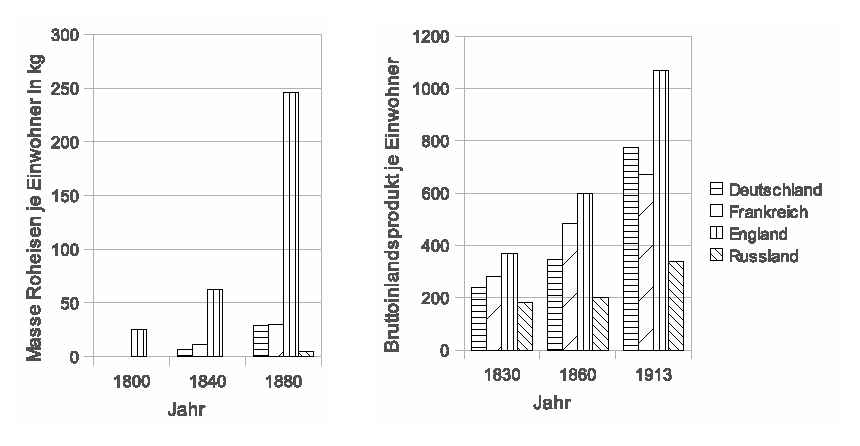
\includegraphics[width=\textwidth]{vorr-gb-diag.eps}
\caption{Roheisenproduktion und Bruttoinlandsprodukt europäischer
Staaten}
\label{pic:vorr-gb-diag}
\end{figure}

\paragraph{Wie Abbildung \ref{pic:vorr-gb-diag} zeigt,} hat
Großbritannien den wirtschaftlichen Entwicklungsprozeß deutlich eher
und mit deutlich höherer Intensität begonnen als andere europäische
Staaten. Es gilt also herauszufinden, wie es zu dieser rasanten
Entwicklung kam.\\

\begin{aufgabe}
Begründen Sie die Vorreiterrolle Englands anhand der besonderen
Voraussetzungen, die dieses Land im Industrialisierungsprozeß
hatte!\footnote{Dazu ist der Inhalt von Abbildung
\ref{pic:vorr-gb-diag} hinreichend}
\end{aufgabe} 

\subsection{Innenpolitische Entwicklung}
\index{Großbritannien!innenpolitisch}

Die \dat{Große Revolution von 1640 bis 1688}
\index{Großbritannien!Große Revolution} \index{Glorious Revolution}
hatte der mittelalterlich"=feudalen Epoche in England ein Ende gesetzt.
Die neue Verfassung sah zensusgebundenes Wahlrecht und
Parlamentssitzvergabe vor und ermöglichte so der \beg{gentry}, den
alten Feudaladel zu verdrängen und ihre fortschrittlichen
wirtschaftlichen Interessen durchzusetzen.

Außerdem sorgte die scharfe Abgrenzung zwischen den Schichten --
Unter-, Oberschicht, Bedienstete etc. -- für eine klare Regelung der
gesellschaftlichen und sozialen Verhältnisse. 


\subsection{Außenpolitische Entwicklung}
\index{Großbritannien!außenpolitisch}

\paragraph{\nam{Henry \Rm{7}} (1486\,--\,1509)} England beginnt eine lange
Tradition der internationalen Seefahrt.

\paragraph{\nam{Elisabeth \Rm{1}} (1558\,--\,1603)} Die englische Flotte
erringt den \dat{Sieg gegen die spanische Armada} und wird so zur
Seemacht. -- Außenhandel und Piraterie weiten sich aus.

\paragraph{\nam{James \Rm{1}} (1603\,--\,1625)} erwirbt 13 Kolonien als
Rohstoffquellen für England und legt so den Grundstein für eine
gezielte Kolonialpolitik.

\paragraph{\Nam{Cromwell, Oliver}{Oliver Cromwell}
(1599\,--\,1658)} England sichert seine Vormachtstellung auf See durch
Siege gegen Holland und Spanien und erwirbt weitere Kolonien, wie zum
Beispiel Jamaika.

\paragraph{\nam{Charles \Rm{2}} (1660\,--\,1685)} Der Krieg gegen
Holland bringt neue Kolonien -- Neuholland und Neuamsterdam.

\paragraph{1714\,--\,1815} Großbritannien erweitert im \dat{War of
Jenkins' Ear 1739\,--\,1742} seinen Kolonialbesitz, erwirbt durch das
Wegfallen Frankreichs als Konkurrenten durch den \dat{Siebenjährigen
Krieg 1756\,--\,1763} Kanada und steigt so endgültig zur Weltmacht
auf.\\

Großbritannien hatte also vor allem durch Handel und Seefahrt einen
gewaltigen Vorrat an Macht, Geld, Rohstoffen, Arbeitern und
Absatzmärkten gewonnen. Dieser bildete die Grundlage für den rasanten
Industrialisierungsprozeß. Abbildung \ref{pic:vorr-gb-gr} bietet
nochmals einen Überblick.

\begin{figure}
\centering
%\begin{sideways}
%\input{vorr-gb-gr.eepic}
%\end{sideways}
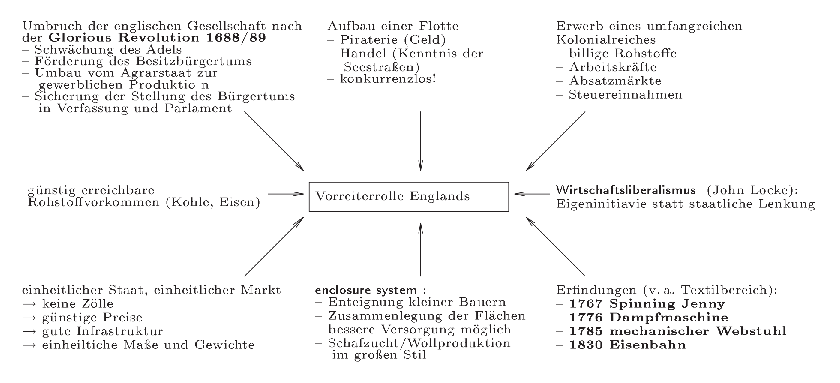
\includegraphics[width=\textwidth]{vorr-gb-gr.eps}
\caption{Ursachen für die Vorreiterrolle Englands}
\label{pic:vorr-gb-gr}
\end{figure}

\endinput

\section{Die Überwindung der Rückständigkeit Deutschlands}
\label{sec:aufh-rueckst-d}
\index{Industrialisierung!Deutschland}

\begin{figure}
\centering
%\begin{sideways}
%\input{vergl-d-e.eepic}
%\end{sideways}
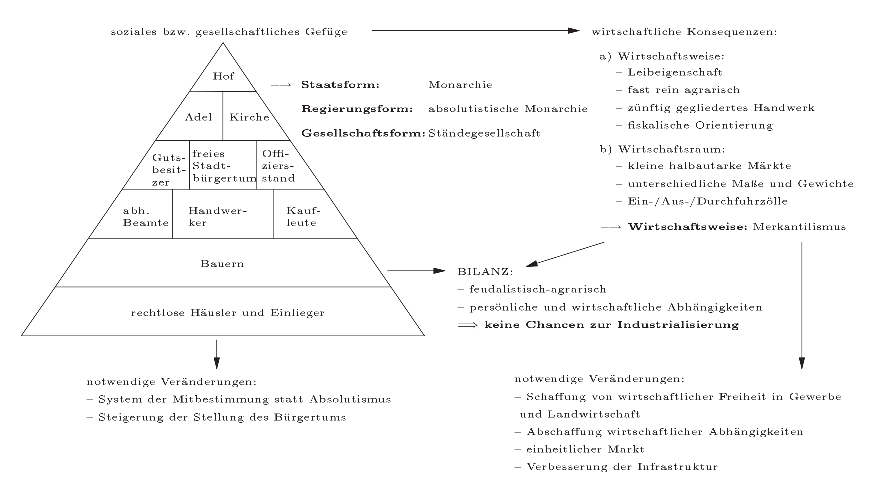
\includegraphics[width=\textwidth]{vergl-d-e.eps}
\caption{Die deutschen Verhältnisse}
\label{pic:dt-verh}
\index{Deutschland!Rückständigkeit}
\end{figure}

\begin{aufgabe}
Zeigen Sie an vier ausgewählten Faktoren, daß Deutschland im
Vergleich zu England als rückständig zu bezeichnen ist!
\end{aufgabe}

\paragraph{Wie Abbildung \ref{pic:dt-verh} zeigt,} waren um 1800
dringend Maßnahmen nötig, um ebenfalls in die industrielle Revolution
einsteigen zu können. Dieser Abschnitt soll zeigen, wie diese
beschaffen waren und was sie bewirkten. \\

\begin{aufgabe}
Stellen Sie an einem Beispiel die Überwindung der Rückständigkeit
Deutschlands im Vergleich zu England dar!
\end{aufgabe}

\subsection[Die Preußischen Reformen]
{Die Preußischen Reformen\footnote{Da die Informationen aus dem im
Geschichtsunterricht gehaltenen Vortrag ungeeignet waren, verwende ich
hier hauptsächlich Material aus \cite{BaswiSchuGesch}.}}
\index{Preußische Reformen}

\mar{Welche Idioten haben damals den Vortrag zu diesem Thema gemacht?}
\begin{aufgabe}
Untersuchen Sie die Preußischen Reformen auf ihre Veränderungen
für das Wirtschaftsgefüge hin!

Fassen Sie sämtliche Informationen zusammen, die zum wirtschaftlichen
Aufschwung Deutschlands als Voraussetzung anzusehen sind und stellen
Sie deren Wirkung dar!
\end{aufgabe}

\paragraph{Nach dem \dat{Krieg gegen Napoleon 1806/1807}} war Preußen
dem Zusammenbruch nahe. Daraufhin initiierten fortschrittliche und
einflußreichende Persönlichkeiten -- allen voran Reichsfreiherr
\Nam{Stein, Karl vom und zum}{Karl vom und zum Stein} und Fürst
\Nam{Hardenberg, Karl August von}{Karl August von Hardenberg} -- eine
Reihe von tiefgreifenden Reformen, die den Wiederaufbau und die
Befreiung des Staates von der französischen Fremdherrschaft
ermöglichen sollten.

Damit einher ging auch eine wirtschaftliche Reform Preußens, dessen
auf dem System der persönlichen Abhängigkeit beruhende Gutswirtschaft
von am Wirtschaftsliberalismus orientierten Grundsätze abgelöst
wurde.

\subsubsection{Bauernbefreiung}
\index{Bauernbefreiung}
\index{Regulierungsedikt}
\index{Oktoberedikt}

Das \dat{Oktoberedikt von 1807} hob die Erbuntertänigkeit und damit
die Leibeigenschaft auf und ermöglichte ihnen den Besitz von eigenem
Land. Die Gutsbesitzer wurden gemäß dem \dat{Regulierungsedikt von
1809} entschädigt.

Der so geschaffene \emph{freie Bauernstand} war nun in den
Wirtschaftsprozeß integriert und also an Produktionssteigerungen
interessiert.

\subsubsection{Städteordnung}
\index{Städteordnung}

Mit der \dat{Einführung der Städteordnung 1808} gewährte Preußen seine
Städten die selbständige Verwaltung ihrer Angelegenheiten. Die Bürger
konnten fortan aktiv und passiv an der an einen niedrigen Zensus
gebundenen Wahl zur Stadtverordnetenversammlung, die
wiederum Magistrat und Bürgermeister (Exekutive) wählte, teil- und
damit auf die Politik Einfluß nehmen.

Dies sind die Ursprünge der kommunalen Selbstverwaltung in Deutschland.

\subsubsection{Verwaltungsreform}
\index{Verwaltungsreform}

Die \emph{Verwaltungsreform} sollte
\textquote[\cite{BaswiSchuGesch}]{einen lestungsfähigen, sparsamen
und bürgernahen Staatsapparat [\dots] schaffen.} Dazu gehörten eine
Vereinfachung der Behördenstruktur durch eindeutige Klärung der
Zuständigkeiten und die Trennung von Justiz und Verwaltung. Möglich
wurde dies durch die neuen Ein"-stel"-lungs- und Laufbahnkriterien für
Beamte (Qualität statt Gunst) und die fortschreitende
Verschriftlichung und Archivierung von Vorgängen. -- Das
Berufsbeamtentum, wie es heute noch fast unverändert in Deutschland
besteht, wurde geprägt. -- Außerdem wurden die Beamten durch relativ
hohe Gehälter bestechungssicher gemacht.\mycite{WikPreusRef}

Ein weiterer bedeutender Inhalt der Verwaltungsreform war die
Schaffung des \emph{klassischen Kabinetts} aus Ministerien (fünf an
der Zahl) mit klar abgegrenzten Ressorts.

\subsubsection{Gewerbereform}
\index{Gewerbereform}

\dat{1810/11 wurde die Gewerbefreiheit} eingeführt. -- Um ein Gewerbe
aufzunehmen genügte der Erwerb eines Gewerbescheins.
\mar{Gewerbe\-steuer? -- Stimmt. Einfügen!} Damit ging die Aufhebung
des Zunftzwangs und somit die Beseitigung zahlreicher Monopole einher.
Dies und die weitgehende Abschaffung der staatlichen Aufsicht über die
Wirtschaft beförderte Konkurrenz und freien Markt.

\subsubsection{Folgen}

\begin{itemize}
\item Unabhängigkeit von den Gutsherren bringt ehemalige Bauern als
Arbeitskräfte in die Städte.
\item zunehmende Bedeutung des Gewerbes auch in ländlichen Gebieten
\item zunehmende Verstädterung
\item später: Verschärfung der sozialen Frage durch übermäßige Zunahme
der Zahl der Handwerker bei starker Konkurrenz
\end{itemize}


%%%%%%%%%%%%%%%%%%%%%%%%%%%%%%%%%%%%%%%%%%%%%%%%%%%%%%%%%%%%%%%%%%%%%%

\subsection{\dat{Die Fr"uhindustrialisierung 1770\,--\,1850}}
\label{ssc:frueh-ind}
\index{Fr"uhindustrialisierung}

\begin{aufgabe}
Stellen Sie Ansätze wirtschaftlichen Aufschwunges in Deutschland
anhand der Frühindustrialisierung dar!

Bewerten Sie die Wirkungsweise dieser auf den
Industrialisierungsprozeß insgesamt!
\end{aufgabe}

\paragraph{Die Verarbeitung von Agrarprodukten} wie sie in
Zuckerfabriken, Branntweinbrennereien, Brauereien, Ölmühlen und
Tabakfabriken betrieben wurde, bildete die Wurzeln des
Unternehmertums. So wurde beispielsweise der Zuckerrübenbauer zum
Zuckerfabrikanten und der Textilverleger zum Textilfabrikanten.

\paragraph{Die Textilproduktion beruhte auf dem Verlagssystem}
(beispielsweise heimgewerbliche Leinenherstellung), das in dieser
Phase der Industrialisierung zur Blüte kam
\mycite[207]{gelbesGeschichts}.  Mit der \dat{Einführung mechanischer
Webstühle 1830} wurden dann die Voraussetzungen für die
Textilindustrie geschaffen.

\paragraph{Ferner erschloß man neue Industriezweige,} wie den
Kohlebergbau und die Erzgewinnung.\\

Diese Ansätze wirtschaftlichen Aufschwungs schufen einen Bedarf nach
Maschinen. -- Kleine Reparaturwerkstätten entwickelten sich zu
Maschinenfabriken. -- Man benötigte Metall. -- Um die isolierten
Produktionsinseln zu verbinden, mußte man die Infrastruktur aufbauen.
-- Man baute 1835 die erste Eisenbahnstrecke. -- Wieder brauchte man
Metall.

Hier zeigen sich die Grundlagen der \beg{Interdependenzen} -- starker
Rückkopplungseffekte, die die folgende rasante Entwicklung
Deutschlands vom Agrar- zum Industriestaat bedingten.

Die Wirtschaft selber entwickelte sich in der Zeit der
Frühindustrialisierung allerdings nur langsam.

%%%%%%%%%%%%%%%%%%%%%%%%%%%%%%%%%%%%%%%%%%%%%%%%%%%%%%%%%%%%%%%%%%%%%%

\subsection{Der Zollverein}
\label{ssc:zollv}
\index{Zollverein}

\begin{aufgabe}
Stellen Sie den Entstehungsprozeß des Zollvereins dar!

Bewerten Sie seine Bedeutung für den Wirtschaftsaufschwung/die
Industrialisierung in Deutschland!
\end{aufgabe}

\subsubsection{Entstehungsprozeß}

\paragraph{Vorläufer:} süddeutscher Zollverein, mitteldeutscher
Handelsverein, preußisch-hessischer Verein

\begin{chronik}
\item[1.\,1.\,1834]
\dat{Zollvereinigungsvertrag} zwischen den Vorläufervereinen -- Der
\emph{deutsche Zollverein} entsteht.

\item[bis 1854]
Westerweiterung durch Anschluß weiterer Länder

\item[1857]
Einführung des Zollvereinstalers

\item[1867]
Norderweiterung

\item[1868]
verbindliche Einführung von \emph{Meter und Kilogramm}
\index{metrisches System}

\item[1871]
Zollverein ist vollständig\footnote{Zur Zusammensetzung des
Zollvereins siehe
\href{http://de.wikipedia.org/wiki/Gebiet_des_Deutschen_Zollvereins}
{diesen Wikipediaartikel}}
\footnote{Österreich wurde trotz Antrages nicht aufgenommen, da das
den Verein dominierende Preußen seine Rivale durch die zusätzlichen
Zahlungen schwächen konnte.}
und umfaßt zur Reichsgründung das gesamte Reichsgebiet
\index{Deutsches Reich}
\end{chronik}


\subsubsection{Politische Bedeutung}

\begin{itemize}
\item ökonomische und materielle Verbindung der Deutschen zu einer
\emph{Nation}
\item Vorbereitung einer echten Nation
\item Stärkung der materiellen Kraft der deutschen Lande durch Wahrung
der auswärtigen Gesamtinteressen
\item Verschmelzung einzelner Provinzialinteressen zu einem
Nationalinteresse -- Erweckung eines Nationalgefühls
\end{itemize}

\subsubsection{Wirtschaftliche Bedeutung}

\begin{itemize}
\item \mar{?} Wiedergeburt des deutschen Unternehmergeistes
\item \mar{?} Teilhabe der deutschen an allen
Nationalangelegenheiten 
\item \mar{?} Anteilnahme des Mittelstandes und der
Großgrundbesitzer an praktischer Politik
\item Grundlage für einheitlichen Markt
\item Wegfall der Zollschranken
\item einheitliche Währung und Maßeinheiten
\end{itemize}

$\Longrightarrow$ Bedingung für ein modernes Wirtschaftssystem


%%%%%%%%%%%%%%%%%%%%%%%%%%%%%%%%%%%%%%%%%%%%%%%%%%%%%%%%%%%%%%%%%%%%%%

\subsection{Der neue Unternehmertypus}
\index{Deutschland!Unternehmertum}

\begin{aufgabe}
Zeigen Sie, daß sich in Deutschland ein neuer Unternehmertypus
Herausbildete und stellen Sie ihn vor!

Begründen Sie, daß er einen Beitrag zur Überwindung der
Rückständigkeit Deutschlands leisten konnte!
\end{aufgabe}

\subsubsection{Entstehung von Unternehmen}

\begin{itemize}
\item Handwerker bauen auf technischen oder finanziellen Grundlagen
oder auf Basis einer Idee Werkstätten zu Fabriken aus.
\item \beg{Feudalunternehmer}
\item Unternehmensgründung auf Basis von Kapitalbesitz oder Erbschaft
(z.\,B. \Nam{Krupp, Alfred}{Alfred Krupp}
\end{itemize}

\subsubsection{Entwicklung zum \emph{neuen} Unternehmer}

Private Unternehmer, Techniker, Kaufleute, Wissenschaftler und
Politiker unternahmen Bildungsreisen nach Großbritannien, von wo sie
Technologien und Anregungen für das deutsche Bildungswesen
mitbrachten. Sie importierten auch britische Maschinen und knüpften
Beziehungen, über welche sie britische Fachleute nach Deutschland
holten.

Hier entwickelte sich eine neue Art, Unternehmen zu gründen: Man
setzte risikofreudig teilweise das gesamte Eigen- oder auch
Familienkapital ein. Wo dieses nicht reichte, schlossen sich mehrere
Unternehmer zusammen -- man gründete Aktiengesellschaften -- oder
wurden Kredite aufgenommen -- Großbanken, wie die \ins{Deutsche Bank}
oder die \ins{Dresdner Bank} entstanden.

\subsubsection{Mitwirkung der Unternehmer bei der Überwindung der
Rückständigkeit Deutschlands}

\begin{description}
\item[Wissen und Erfahrung:] Import von technischen Neuerungen,
Maschinen, Facharbeitern und Ingenieuren
\item[Bildungssystem:] Übergang zu innerdeutscher Ausbildung von
Fachkräften und Ingenieuren an Fachschulen und technischen Hochschulen
\item[Aufschwung des Finanzwesens:] hohe private Investitionen und
damit verbundenes Risiko
\item[technischer Fortschritt:] Kapitalismus führt zu hohem
Konkurrenzdruck -- Unternehmen verbessern eigenständig Produktions-
und Verarbeitungsprozesse. (forschendes Unternehmertum)
\end{description}

Damit war bald sowohl die finanzielle wie auch die technologische
Unabhängigkeit vom Ausland gewährleistet. Die neuen Unternehmer trugen
so maßgeblich zum Aufbau eines wirtschaftlich konkurrenzfähigen
deutschen Kaiserreiches bei.

%%%%%%%%%%%%%%%%%%%%%%%%%%%%%%%%%%%%%%%%%%%%%%%%%%%%%%%%%%%%%%%%%%%%%%

\subsection[Veränderungen in der Infrastruktur]
{Veränderungen in der Infrastruktur \mycite[157/158]{braunesGeschichts}}

\begin{aufgabe}
Weisen Sie nach, daß eine Verbesserung der Infrastruktur in
Deutschland stattgefunden hat!

Bewerten Sie die Bedeutung dessen für den Industrialisierungsprozeß!
\end{aufgabe}

\paragraph{Die Verbesserung der deutschen Infrastruktur} begann in der
Zeit der Frühindustrialisierung: Man befestigte die Landstraßen, baute
Flüsse aus und verband sie durch Kanäle. Dampfschiffe erleichterten
und beschleunigten den den Gütertransport.

\paragraph{Die weitaus bedeutendste Veränderung} war aber die
Einführung der Eisenbahn \index{Eisenbahn} in Deutschland. Nur
sinnvoll durch den Zollverein (\emph{siamesische Zwillinge}) erfuhr
sie seit ihrem \dat{ersten Einsatz 1935} eine rasante
Entwicklung\footnote{Zu konkreten Zahlen siehe
\cite[159]{braunesGeschichts} und \cite{WikEisenbahn}} und wurde zum
entscheidenden Motor der Industrialisierung.

Einerseits erleichterte, beschleunigte und verbilligte sie den
Personen- und Warenverkehr erheblich. Dadurch eröffneten sich nicht
nur neue Möglichkeiten, Rohstoffe zu beschaffen beziehungsweise
Produkte zu vertreiben, sondern förderte ebenso den kulturellen
Austausch und vergrößerte die Anzahl der Arbeiter in Form von
Pendlern.

Andererseits befeuerte die neue riesige Nachfrage nach Stahl für
Schienenverlegung und Eisenbahnherstellung die Schwerindustrie und den
Arbeitsmarkt. Deren Expansion verlangte wiederum nach weiterem Ausbau
der Eisenbahn und so weiter. -- Diese äußerst starke
\beg{Interdependenz} führte in der Folge den sprunghaften Anstieg der
Wirtschaftsmacht Deutschlands.



%%%%%%%%%%%%%%%%%%%%%%%%%%%%%%%%%%%%%%%%%%%%%%%%%%%%%%%%%%%%%%%%%%%%%%

\subsection{Entstehung von Industriegebieten -- Das Ruhrgebiet}
\index{Industriegebiete!Entstehung}
\index{Ruhrgebiet}

\begin{aufgabe}
Zeigen Sie am Beispiel des Ruhrgebietes die schrittweise Entstehung
industrieller Ballungsgebiete!

Bewerten Sie die Bedeutung solcher Ballungsgebiete für den
Industrialisierungsprozeß!
\end{aufgabe}

\subsubsection[Entstehungsprozeß]{Entstehungsprozeß\footnote{Hier am
Beispiel des Ruhrgebiets. -- In anderen Gebieten ähnlich.}}

\begin{enumerate}
\item heranwachsende Stahlindustrie seit 1820 -- Strukturwandel von
Landwirtschaft zu Industrie nach Kohlefunden
\item 1840\,--\,1848 Ausbau von Eisenbahn und Binnenschiffahrt führt
zur Verbesserung der Infrastruktur
\item Übergang vom Stollen- zum Schachtbau
\item Eröffnung von Zechen in großer Zahl führt zu starker Zuwanderung
\item Eisenindustrie ab 1850, forcierte Entwicklung durch Eisenbahnbau
\item 1850\,--\,1870: Kohle!
\item Land- und Intensivwirtschaft zur Versorgung der Bevölkerung in
den Randgebieten der Ballungszentren
\item Nachfolgeindustrien
\end{enumerate}

\subsubsection{Bedeutung der Ballungsgebiete für den
Industrialisierungsprozeß}

\begin{itemize}
\item kein Zoll
\item kürzere Transportwege
\item Zusammenarbeit der Unterhehmen
\item Konzentration von Fachpersonal
\item Konzentration von Wissenschaft und Forschung
\item Investition der Rendite in neue Techniken, Betriebe etc.
\end{itemize}

$\Longrightarrow$ Sprungbrett für die Industrialisierung des gesamten
Landes

\endinput



\chapter{Die \emph{Soziale Frage} und Ansätze für deren Lösung}
\label{chp:soziale-frage}
\index{Soziale Frage}

\begin{aufgabe}
Die Industrielle Revolution wird in der historischen Betrachtung als
Segen und Fluch bezeichnet. Nehmen Sie zu dieser Sichtweise wertend
Stellung! 
\end{aufgabe}

\section{Die Entstehung der Arbeiterschaft als Klasse}
\label{sec:arb-klas-entst}
\index{Arbeiterklasse}

\mar{irgendwie mehr Geographie -- Wo bleiben die Arbeiter?} Ausgehend
von der \dat{Bevölkerungsexplosion ab circa 1800}, deren Ursachen die
Aufhebung der ländlichen Eheverbote, medizinische und
landwirtschaftliche Fortschritte waren und die sich zu einem sich
selbst erhaltenden Prozeß entwickelte, führte die Industrielle
Revolution zu einem \emph{sozialen Wandel}. Dieser schlug sich in der
Herausbildung von Abwanderungs- (vor allem ländliche Regionen wie
Ostpreußen) und Zuwanderungsgebieten (Ballungszentren wie das
Ruhrgebiet) und in der Entstehung von Großstädten und Städten
allgemein nieder.

Dieser Prozeß der \emph{Urbanisierung} ging einher mit der
Herausbildung der Arbeiterklasse, die den Hauptanteil an der
Binnenmigration hatte.

\endinput

\section{Die soziale und gesellschaftliche Lage der Arbeiterschaft
während der Industrialisierung}
\label{sec:soz-ges-lag-arb}
\index{Arbeiterklasse!soz. und ges. Lage}

\subsection{Wohn- und Lebensverhältnisse}

\begin{itemize}
\item Wohnungsknappheit durch rasantes Bevölkerungswachstum
$\Rightarrow$ Bau von \beg{Mietskasernen}:

\begin{itemize}
\item kleinste dunkle feuchte (meist Einraum-) Wohnungen $\Rightarrow$
keine Privatsphäre
\item miserable sanitäre Verhältnisse (eine Toilette für 50 Personen)
\item kaum Heizung
\item Schlafgängertum
\end{itemize}

\item mangelnde Hygiene, Krankheiten, Seuchen
\item Familienväter oft betrunken:

\begin{itemize}
\item Lösung familiärer Konflikte oft mit Gewalt
\item keine Erziehungsinstanz
\item keine Vorbilder für die Heranwachsenden
\end{itemize}

\item schlechte Erziehung und fehlende Schulbildung $\Rightarrow$ kaum
Chancen auf sozialen Aufstieg, Kriminalität
\end{itemize}

\subsection{Arbeitsverhältnisse}

\begin{itemize}
\item Hohe Spezialisierung der Arbeit führte zu Produktivitäts- und
Qualitätssteigerung, aber auch zu Sinnentleerung, Stupidität und
Monotonie.
\item härteste Arbeitsbedingungen
\item hohes Unfallrisiko
\item keine Versicherung
\item kein Kündigungsschutz
\item überlange Arbeitszeiten (bis zu 16 Stunden an sechs Tagen in der
Woche)
\item Hungerlöhne
\item Arbeiterheer führte zu Lohndumping. -- Selbst Kinder mußten
arbeiten.
\end{itemize}

Es entstand also eine neue Zweiklassengesellschaft mit der besitzenden
Klasse, deren Attribute Reichtum, politische und wirtschaftliche Macht
waren, auf der einen Seite und der arbeitenden Klasse, die durch
Massenverelendung und -armut gekennzeichnet war, auf der anderen.

Allerdings muss man dazusagen, dass es auch in der Arbeiterklasse
Standesunterschiede gab. So standen die Facharbeiter, deren äußeres
Kennzeichen der Hut war über den älteren (30\,--\,40 Jahre) und den
jüngeren einfachen Arbeitern. Diese hatten eine Mütze auf dem Kopf.
Auf der untersten Stufe standen die Tagelöhner, die keinerlei feste
Anstellung hatten. Die Entlohnung und die Qualität der
Lebensverhältnisse lief proportional zu dieser Rangordnung. Die Folge
waren starke Spannungen und Uneinigkeit innerhalb dieser
Klasse\footnote{Den Facharbeiter ging es beispielsweise recht gut. Da
sie außerdem Macht über die anderen Arbeiter besaßen, waren sie
verhaßt.} Das behinderte die Arbeiter bei ihrem späteren Kampf für
bessere Lebensverhältnisse und verzögerte die Lösung der sozialen
Frage.

\endinput

\section[Die soziale Frage nach \Nam{}{Hegel}]
{Die soziale Frage nach \Nam{}{Hegel}\mycite{HegelGrundl}}
\label{sec:soz-frag-heg}
\index{Soziale Fragel!nach Hegel}
\Nam{Hegel, Georg Wilhelm Friedrich}{}

Zur Problematik der sozialen Frage nach \Nam{}{Hegel} siehe die Abbildungen
\ref{pic:soz-frag-sch} und \ref{pic:soz-frag-sch-rev}.

\begin{figure}
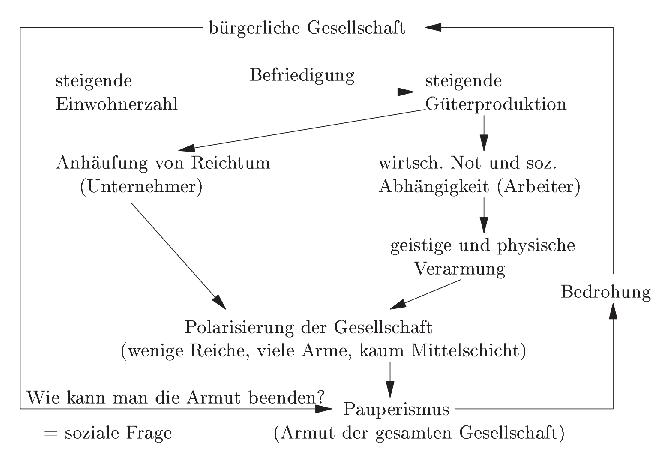
\includegraphics[width=\textwidth]{soz-frag-sch.eps}
\caption{Entstehung der sozialen Frage nach \Nam{}{Hegel}}
\label{pic:soz-frag-sch}
\end{figure}

\begin{figure}
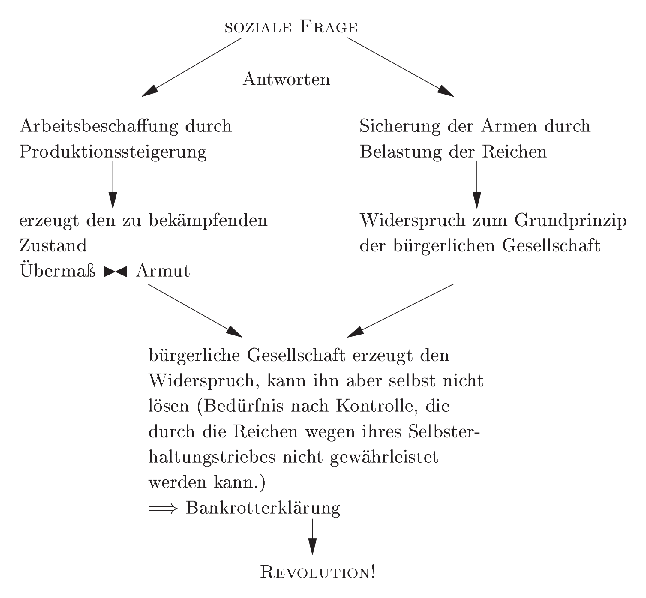
\includegraphics[width=\textwidth]{soz-frag-sch-rev.eps}
\caption{Folgen der sozialen Frage nach \Nam{}{Hegel}}
\label{pic:soz-frag-sch-rev}
\end{figure}

\endinput

\section{Lösungsansätze für die soziale Frage}
\label{sec:soz-frag-loes}
\index{soziale Frage!Lösungsansätze}

\begin{aufgabe}
Stellen Sie einen Maßnahmenkomplex zur Abmilderung/Lösung der Sozialen
Frage vor und prüfen Sie seine Wirksamkeit anhand Hegels Auffassungen! 
\end{aufgabe}

\subsection{Der Marxismus -- Veränderung durch Umbruch}
\label{ssc:marxismus}
\index{Marxismus}
\index{Materialismus}
\mar{\cite{DudPolGes} bietet hier eine gute Darstellung.}

\begin{aufgabe}
Erarbeiten Sie aus der Quelle Marx' Sicht auf die Rolle der
Bourgeoisie in der Geschichte!

Untersuchen Sie die Richtigkeit der fettgedruckten Position anhand des
kapitalistischen Produktionsprozesses in Marx' sogenannter \jar{Basis}! 

Überprüfen sie anhand des Hegelschen Systems der Sozialen Frage,
inwiefern die Ideen Marx' eine Lösung dieser darstellen!
\end{aufgabe}

Im Hefter ist dies in vorerst ausreichender Form dargestellt.

%%%%%%%%%%%%%%%%%%%%%%%%%%%%%%%%%%%%%%%%%%%%%%%%%%%%%%%%%%%%%%%%%%%%%%

\subsection{Die Arbeiterschaft -- Hilfe zur Selbsthilfe}
\label{ssc:arb-bew}
\label{ssc:soz-frag-loes-arb}
\index{Arbeiterbewegung}

\begin{aufgabe}
Untersuchen Sie, inwiefern die Gewerkschaften zur Lösung der sozialen
Frage beitrugen!
\end{aufgabe}

\subsubsection{Ausgangspunkt}

Der Vorteil der Arbeiter war, daß sie eine äußerst breite Schicht der
Bevölkerung bildeten. Unter der Voraussetzung, daß sie sich
zusammenschließen und als die Masse handeln, die sie waren, kann man
ihnen große Chancen, ihre Ziele und Interessen durchzusetzen,
einräumen.

Genau diese Voraussetzung ist aber das Problem, denn die Arbeiter
waren keine homogene Masse. Vielmehr gab es auch hier eine soziale
Schichtung, die sich in der Gehaltsstruktur ausdrückte und zum
ständigen Konflikt beispielsweise zwischen Meistern und
\glq{}Angelernten\grq{} führte. Das ständig bereitstehende
\emph{Ersatzheer} führte zu großer Konkurrenz untereinander. Dieses
Konfliktpotential wurde noch durch die Fabrikordnungen vergrößert,
denn diese sahen Kollektivstrafen vor.

Zur unterschiedlichen sozialen kam noch die unterschiedliche regionale
Herkunft. Da es der Arbeiterschaft an organisatorischem Wissen fehlte,
war es auch hier schwer, eine breite Basis für die Durchsetzung der
Ziele zu finden.

Die Lebensumstände der Arbeiter waren weiterhin schon so miserabel,
dass diese entweder gar keine Zeit fanden, sich um andere Probleme als
ihre eigenen, zu kümmern oder die ständigen Sorgen von vornherein in den
Alkohol oder den Sport flohen.\\


\subsubsection{Entwicklung der Arbeiterbewegung in Großbritannien}
\index{Arbeiterbewegung!Großbritannien}

\begin{chronik}
\item[nach 1814/15] zunehmende Politisierung des Aufbegehrens der
Arbeiter, Streiks

\item[1824] Aufhebung des Koalitionsverbots, Bildung von
Gewerkschaften und Gewerkschaftsverbänden in der Folge

\item[1840] Aus der chartistischen\footnote{Der Name \emph{Chartismus}
leitet sich aus dem Gesetzentwurf ab, der dieser Strömung entstammte
und Forderungen nach beschränkungslosen (Zensus etc.) jährlichen
geheimen allgemeinen Wahlen, Diäten für Abgeordnete und anderem
umsetzen sollte.} Strömung entstand die \ins{National
Chartist} als erste allerdings illegale Arbeiterpartei unserer Zeit.

\item[1860] Nachdem die politische Richtung der Arbeiterbewegung ins
Stocken gekommen war, bildet sich aus den entstehenden \emph{Trade
Unions} (Gewerkschaften) der \ins{Trade Union Council}.

\item[1864] Gründung der \ins{Internationalen
Arbeiterassoziation}\footnote{\Nam{Marx, Karl}{Karl Marx} war
eines der führenden Mitglieder.} (IAA) als Zusammenschluss aller
Arbeiterorganisationen

\item[1876] Auflösung der IAA nach Erfüllung ihrer Aufgabe,
Fortsetzung der Arbeit in Parteien
\end{chronik}


\subsubsection{Arbeiterparteien in Deutschland}
\index{Arbeiterparteien!Deutschland}
\mar{Zur Entwicklung siehe vorerst das Organigramm im Hefter.}

Ziele/Forderungen:

\begin{itemize}
\item Brechung des \Beg{Ehernes Lohngesetz}{Ehernen
Lohngesetzes}\footnote{Da \cite{WiLexEhLohnGes} eine andere Definition
bringt, als ich im Glossar niedergeschriebenen habe, ist fraglich, ob
der hier abgedruckte Sachverhalt stimmt.}
\item allgemeine, gleiche, direkte Wahl (Druckmittel gegen
Unternehmer)
\item Befreiung der Arbeiterklasse durch die Arbeiterklasse
\item Besetitigung der Abhängigkeit des Lohnarbeiters
\item politische Freiheiten (Voraussetzung für ökonomische
Freiheiten)
\item marxistische Strömungen: Revolution \index{Marxismus}
\item politisch-praktische Strömungen: Reformen
\end{itemize}

Mittel:

\begin{itemize}
\item Parteibildung und -arbeit
\item Wahlrechtskämpfe
\item Zusammenschluss von Arbeiterorganisationen
\item Gründung von Arbeiterproduktivgenossenschaften (Vorschlag
\Nam{Lassalle, Ferdinand}{Lassalle}s) -- Arbeiter selbst als
Unternehmer
\item Programme, Zeitschriften
\end{itemize}


\subsubsection{Gewerkschaften in Deutschland\mycite{MustaGeGe}}
\index{Gewerkschaften!Deutschland}

Die deutsche Gewerkschaftsbewegung wies einige Unterschiede zu der in
Großbritannien auf. So wurde in Deutschland durch späte Einführung des
Koalitionsrechts und Sozialistengesetz ein erheblicher Druck ausgeübt.
Dies führte dazu, dass die Vereinigungen im Untergrund
weiterexistieren mussten. Dadurch zu kluger Planung und Organisation
gezwungen, erfuhren die Gewerkschaften eine Stärkung.

Weiterhin waren die deutschen Gewerkschaften ideologisch breiter
aufgestellt. Das bedeutete natürlich, dass alle ihre
Interessenvertretung fanden, hatte aber auch den Nachteil, dass die
Möglichkeiten, als Masse zu handeln, eingeschränkt waren.

Letztendlich legte man in Deutschland sehr großen Wert auf die
organisatorische Trennung zwischen Gewerkschafts- und Parteiarbeit.
-- Die Gewerkschaften übernahmen die überparteiliche soziale
Unterstützung und Basisarbeit während politische und parlamentarische
Arbeit den Parteien zufiel. Man suchte so, die Sorge für die Lage der
Arbeiter unabhängig von politischen Meinungsverschiedenheiten zu
machen, rief die Arbeiter aber gleichzeitig auf, durch Parteieintritt
den Einfluss des Proletariats auf das Staatsgeschehen zu
vergrößern.\mycite{ResErfGeKo} \mycite{ResKonfGeVoGo}\\

\noindent Entwicklung:

\begin{chronik}
\item[nach 1848/49] lokale Arbeiterkomitees und -zusammenschlüsse

\item[1868] Gründung des \Ins{Allgemeiner Deutscher
Arbeiterschaftsverband}{Allgemeinen Deutschen
Arbeiterschaftsverbandes}

\item[1868] Gründung der \Ins{}{\Nam{Hirsch, Max}{Hirsch}-\Nam{Duncker,
Franz}{Duncker}schen-Gewerksverbände}\footnote{\cite{LEMOHiDu} datiert
hier auf 1869.}

\item[1869] Gründung der \Ins{Internationale
Gewerksgenossenschaften}{Internationalen Gewerksgenossenschaften}
durch \Nam{Bebel, August}{August Bebel} und \Nam{Liebknecht,
Wilhelm}{Wilhelm Liebknecht}

\item[1869] Koalitionsfreiheit für Preußen

\item[1878] \ges{Gesetz gegen die gemeingefährlichen Bestrebungen der
Sozialdemokratie} -- Weiterexistenz im Untergrund

\item[1886] Streikerlass in Preußen -- Verfolgung illegaler
Gewerkschaften

\item[1890] Aufhebung des Sozialistengesetzes

\item[1890] Gründung der \ins{Generalkommission der Freien
Gewerkschaften Deutschlands} als erster Dachorganisation für
sozialistische Gewerkschaften auf Initiative von \Nam{Legien,
Carl}{Carl Legien}

\item[1891] Gründung des \Ins{Deutscher
Metallarbeiterverband}{Deutschen Metallarbeiterverbandes} -- erste
Industriegewerkschaft

\item[1890er] Gründung christlicher Gewerkschaften, Formierung zum
Verband \mar{Irgendwie stimmen hier einige Zahlen nicht.}
\end{chronik}

Ziele:

\begin{itemize}
\item soziale Ziele --Loslösung von politischen Fragestellungen
\item kürzere Arbeitszeit
\item höhere Löhne
\item Abbau der Frontstellung des Proletariats gegen das Bürgertum
(Hirsch-Duncker)
\item Förderung und Wahrung der Würde und des materiellen Interesses
der Arbeiter
\end{itemize}

Mittel:

\begin{itemize}
\item Streik
\item lokale Komitees und Arbeiterzusammenschlüsse $\longrightarrow$
Gewerkschaften $\longrightarrow$ Gewerkschaftsverbände
\item Presseorgane
\item Kassen zur Unterstützung von Arbeitslosen, Not leidenden,
Kranken, Invaliden, Alten, Wandernden
\end{itemize}

\newpage
%%%%%%%%%%%%%%%%%%%%%%%%%%%%%%%%%%%%%%%%%%%%%%%%%%%%%%%%%%%%%%%%%%%%%%

\subsection{Die Rolle der Unternehmer}
\label{ssc:soz-frag-loes-unt}

\subsubsection{Maßnahmen}

% Breite der ersten Spalte der Tabelle
\newlength{\frstcol}
\settowidth{\frstcol}{\textsc{Harkort}}
\addtolength{\frstcol}{1ex}

% Breite der zweiten und dritten Spalte der Tabelle
\newlength{\sndthrdcol}
\newlength{\wholecols} % Breite von zweiter und dritter Spalte zusammen
\setlength{\wholecols}{\textwidth}
\addtolength{\wholecols}{-\frstcol}
\addtolength{\wholecols}{-5\tabcolsep}
\setlength{\sndthrdcol}{0.5\wholecols}



\tablefirsthead{
\toprule
Untern. & fürsorglicher Charakter & unterdrückender Charakter \\
\midrule}
\tablelasttail{\bottomrule}

\begin{supertabular*}{\textwidth}%
{p{\frstcol}p{\sndthrdcol}p{\sndthrdcol}}
\vspace{0.01pt}
\Nam{Stumm-Halberg, Carl Ferdinand Freiherr von}{Stumm}
& \begin{tablist}
\item Schulen
\item Verantwortlichkeit für außerfabrikale Arbeiterhandlungen
\item Ausschluss von Kinderarbeit
\item niedrigvermietete Werkswohnungen
\item Bibliotheken, Park für die Arbeiter, Militärkapellen
\item Kantinen, Teuerungszulagen
\item Bestrafungs- und Entlassungserlaubnis
\item Sprechstunden für die Belegschaft
\item überdurchschnittliche Löhne
\item protektorale Betriebsverfassungen
\end{tablist}
\noindent $\Longrightarrow$ Schutz der Arbeiter
& \begin{tablist}
\item Heiratserlaubnis nach Eigenschaften und Gesundheit der Partner,
Vorbeugung von Arbeitsausfall während Schwangerschaften
\item Erziehungsüberwachung
\item Zwang zum Kirchenbesuch
\item Arbeiter als geborene Untertanen (\emph{König Stumm})
\index{König Stumm}
\end{tablist}
\noindent $\Longrightarrow$ Eindringen in das Privatleben
\\

\vspace{0.01pt}
\Nam{Krupp, Alfred}{Krupp}
& \begin{tablist}
\item überdurchschnittliche Löhne
\item Betriebskrankenkasse
\item Sterbegelder an Hinterbliebene
\item Werkswohnungen
\item Arbeiterpensionskasse -- Altersabsicherung
\item \ins{Gemeinschaft der Kruppianer} -- Stammbelegschaft
\end{tablist}
& \begin{tablist}
\item Nutzung des \beg{Ersatzheeres}
\item Entlassung als Druckmittel
\item Entlassung bei Parteihörigkeit
\item Betäubung von sozialdemokratischen und gewerkschaftlichen
Bestrebungen
\item leistungsabhängige Entlohnung
\item Strafgelder
\item Beitrittspflicht zur Betriebskrankenkasse
\end{tablist}
\\

\vspace{0.01pt}
\Nam{Harkort, Friedrich}{Harkort}
& \begin{tablist}
\item betriebsinterne Sparkassen -- Sicherung von Grunderwerb
\item Bildungssystem für Kinder und Erwachsene -- geistliche,
sittliche und staatsbürgerliche Bildung seiner Angestellten
\item Ablehnung von Kinderarbeit
\end{tablist}
&\vspace{0.01pt} keine klassische Unterdrückung
\\
\end{supertabular*}

\ \\

Ein weiteres bedeutendes Unternehmen, in dem man die Lage der Arbeiter
zu bessern versuchte, war \ins{Carl Zeiss Jena}. Dabei waren die
dortigen Maßnahmen einmal und auch völlig andere als bei den oben
Aufgeführten.

\endinput



\chapter[Fortentwicklung der Industrialisierung in der ersten Hälfte
des 20. Jh.] {Fortentwicklung der Industrialisierung in der ersten
Hälfte des 20. Jahrhunderts}
\label{chp:fortentw-indust}

\section{Neue gesellschaftliche Schichtung}
\label{neue-ges-schicht}
\index{Gesellschaft}
\index{Agrargesellschaft}
\index{Industriegesellschaft}
\index{Dienstleistungsgesellschaft}

Die Gesellschaft in Deutschland entwickelte sich seit dem \dat{Ende der
Agrargesellschaft 1850} über die Industriegesellschaft zur
\dat{Dienstleistungsgesellschaft ab 1990}.

Dabei kann man drei große Linien erkennen: \emph{Urbanisierung}
\index{Urbanisierung}, \emph{Trennung von Arbeit und Leben}
beziehungsweise Hausgemeinschaft und Arbeitsstätte und eine zunehmende
\emph{Differenzierung der Arbeitnehmergesellschaft} in \beg{Arbeiter}
und \beg{Angestellte}. Außerdem setzte um 1900 die Bürokratisierung
ein. \index{Bürokratisierung} 

\endinput

\section{Neue Leitsektoren}
\label{sec:neue-leits}
\index{Leitsektor}

\subsection[Chemische Industrie]{Chemische Industrie\footnote{Die
Grundlage dieses Abschnitts ist ein schnell im Rahmen des Unterrichts
im Internet recherchierter Kurzvortrag. Da dieses Thema weniger
relevant ist, beschränke ich mich bei der Literatur auf die
Wikipedia-Artikel \cite{WikChemInd}, \cite{WikFarbst}, \cite{WikHaBoVerf}, \cite{WikStaudi} und \cite{WikSteikohteer}.}}
\label{ssc:chem-ind}
\index{Chemische Industrie}

\mar{Warum galt die chemische Industrie in jener Zeit als Friedens-
und damit Staatserhaltend?}
In der ersten Hälfte des 19. Jahrhunderts wurden Verfahren erfunden,
den bei der Gasherstellung anfallenden \emph{Steinkohlenteer}
\index{Steinkohlenteer} nutzbringend zu verwenden. Die neuen Produkte
-- allen voran \emph{Anilin} und \emph{Phenol}
\index{Anilin}\index{Phenol} -- waren Grundstoff für zahlreiche
Synthesen. -- Damit war der Aufstieg der Farbenindustrie eingeleitet.

Es wurden Möglichkeiten gefunden, Medikamente, Düngemittel und
Sprengstoffe künstlich herzustellen. Dadurch konnten bisher unheilbare
Krankheiten geheilt und die landwirtschaftliche Produktion erheblich
gesteigert werden. -- Gesundheits- und Versorgungszustand der
Bevölkerung verbesserten sich erheblich, sodass auch die Nachfrage
nach den immer vielseitigeren Produkten der chemischen Industrie
stieg.

Die enge Kooperation dieses Industriezweigs mit technischen
Hochschulen verbesserte das Bildungssystem und trieb die Forschung
voran. So kam es zu weiteren bedeutenden Erfindungen:

\dat{1910} wurde das \dat{\emph{\Nam{Haber, Fritz}{Haber}-\Nam{Bosch,
Carl}{Bosch}-Verfahren}} \index{Haber-Bosch-Verfahren} erfunden,
welches die Synthese von Ammoniak ermöglichte. Dieser dient als
Grundlage für Sprengstoffe und Kunstdünger. Die Verfügbarkeit neuer
Düngemittel bewirkte neue Forschungen in der Landwirtschaft.

\dat{1922} stellte \Nam{Staudinger, Hermann}{Hermann Staudinger} die
These auf, dass Polymere aus Makromoleküle bestehen und begründete
damit die Polymerchemie. Dies führte zur \dat{großtechnischen
Produktion zahlreicher Kunststoffe ab 1930} (beispielsweise
Polystyren, Polyvinylchlorid, Nylon, Buna). Die \dat{1925 gegründete}
\beg{IG Farben} war hier marktführend.

%%%%%%%%%%%%%%%%%%%%%%%%%%%%%%%%%%%%%%%%%%%%%%%%%%%%%%%%%%%%%%%%%%%%%%

\subsection[Elektroindustrie]{Elektroindustrie\footnote{Dieser und die
folgenden vier Abschnitte entstammend Kurzvorträgen, die ich nicht
selbst gehalten habe und deswegen auch keine Quellen angeben kann.}}
\label{ssc:el-ind}
\index{Elektroindustrie}

\begin{chronik}
\item[ab 1900]
erste kommerzielle Sende- und Empfangsanlagen

\item[1904]
erste Röhrendiode -- Gleichrichtung\index{Röhrendiode}

\item[1906]
erste Triode -- Grundlage für Radio und andere Unterhaltungselektronik 
\index{Triode}

\item[1926\,--\,1931] Entwicklung des Fernsehens\index{Fernsehen}

\item[1900\,--\,1950] auch international marktbeherrschende Stellung
von \beg{AEG} und \beg{Siemens}

\item[1931]
Erfindung des Elektronenmikroskops\index{Elektronenmikroskop}

\item[1941]
Erfindung des Computers (Z\,3)\index{Computer}\index{Z\,3}
\end{chronik}

Diese Entwicklungen läuteten des Computer- und Informationszeitalter
ein: Die neuen Möglichkeiten erweckten sofort großes in der
Bevölkerung, in der Politik und beim Militär, sodass sich die Anzahl
der Arbeitsplätze von \dat{80\,000 Beschäftigten 1900} bis \dat{1950
auf 650\,000} steigerte.

%%%%%%%%%%%%%%%%%%%%%%%%%%%%%%%%%%%%%%%%%%%%%%%%%%%%%%%%%%%%%%%%%%%%%%

\subsection{Fahrzeugbau}
\label{ssc:fahrzbau}
\index{Fahrzeugbau}

Sich aus dem Waggonbau entwickelnd erfuhr dieser Industriezweig in
Folge der \dat{Forderung \Nam{Hitler, Adolf}{Hitler}s} nach einem
Wagen für breite Schichten \dat{1934} großen Aufschwung. So wurde
\dat{1937} die \dat{\ins{Gesellschaft zur Vorbereitung der Deutschen
Volkswagen mbH} gegründet}, \dat{1938 in \ins{Volkswagen GmbH}}
umbenannt.

Das Werk wurde im gleichen Jahr in \ort{Wolfsburg}
errichtet.\index{VW} Es war äußerst günstig gelegen: In der Mitte
Deutschlands mit Anbindung an Autobahn, Eisenbahn und durch den
Mittellandkanal ebenfalls an Wasserstraßen. Außerdem waren Stahlwerke,
beispielsweise in \ort{Salzgitter} nicht fern. Im Krieg leisteten hier
20\,000 Kriegsgefangene und KZ-Insassen Zwangsarbeit.
\index{Zwangsarbeit}

Bei der Produktion des neu entwickelten
\emph{KdF-Wagens}\index{KdF-Wagen}, heute als \emph{VW Käfer}\index{VW
Käfer} bekannt, orientierte man sich am
\emph{Fließbandbetrieb}\index{Fließbandproduktion}, wie er bei
\ins{Ford} in \ort{Detroit} praktiziert wurde. Das neue Auto konnte
vier Personen transportieren, war zuverlässig, einfach reparierbar und
billig. So konnte man die Wirtschaft ankurbeln und die Verwendung beim
Militär war auch möglich.  Im Krieg stand dann auch die
Rüstungsproduktion im Vordergrund.  \index{Rüstung}

Nach dem Krieg war das VW-Werk der britischen Militärregierung
\index{Militärregierung} unterstellt, die die Umstellung auf
Zivilproduktion veranlasste.

\endinput

\section{Fließbandarbeit}
\label{ssc:fliessbarb}
\index{Fließbandarbeit}

Die Arbeitswelt in der ersten Hälfte des 20. Jahrhunderts war geprägt
vom \beg{Taylorismus}, der in Kombination mit dem Fließbandbetrieb die
Massenproduktion ermöglichte.

Dieses neue Prinzip der Trennung von geistiger und körperlicher Arbeit
half bei der Lösung sozialer Probleme und versprach \jar{Wohlstand für
alle}. Der anfängliche Enthusiasmus wich aber bald der
Unzufriedenheit: Durch die Monotonie der Arbeit stellten sich
gesundheitliche Probleme ein. Außerdem konnten sich die Arbeiter nun
kaum noch mit ihrem Betrieb und den Erzeugnissen identifizieren, weil
sie das Endprodukt kaum noch zu Gesicht bekamen.

Die Qualität litt und die Motivation fehlte. Es kam zu Konflikten mit
den Arbeitgebern; wo es möglich war wanderten die Arbeitnehmer in den
Dienstleistungssektor ab.

\endinput

\section{Arbeitsbedingungen in der ersten Hälfte des 20. Jahrhunderts}
\label{sec:arb-bed-20jh}

Die Arbeitswelt in der ersten Hälfte des 20. Jahrhunderts war auch
geprägt von miserablen Arbeitsbedingungen: \emph{Niedrige
Mindestanforderugen}, \emph{fehlende Aufstiegschancen}, 
\emph{hohe Fluktuation}, \emph{niedrige Löhne} und \emph{geringe
Arbeitsplatzsicherheit} machten den Arbeitern das Leben schwer.

Doch man tat auch einiges, um jene Bedingungen zu verbessern.  Gab es
um \dat{1900} wenigstens einige \dat{Herbergen für Wanderarbeiter},
brachte das \dat{\emph{\Nam{Stinnes, Hugo}{Stinnes}-\Nam{Legien,
Carl}{Legien}-Abkommen} vom 15.\,11.\,1918} große Fortschritte. Der
aus Furcht vor einer Vergesellschaftung der deutschen Industrie im Zuge
der Novemberrevolution zwischen Gewerkschafts- \Nam{}{Legien} und
Industrievertretern \Nam{}{Stinnes} geschlossene Vertrag legte die
Zusammenarbeit von Arbeitnehmern und -gebern fest. Die Arbeitgeber
verpflichteten sich so, die Rolle der Gewerkschaften als Vertreter der
Arbeiterinteressen anzuerkennen und sie als gleichberechtigte
Tarifpartner zu betrachten. Außerdem wurde der \emph{Achtstundentag}
bei vollem Lohnausgleich eingeführt.
\index{Arbeitnehmer}
\index{Arbeitgeber}
\index{Gewerkschaft}
\index{Tarifverhandlung}
\index{Achtstundentag}

Damit wurden ab 1918/1919 in allen Branchen \emph{Tarifverträge},
Regelung der Arbeitsbedingungen durch \emph{Kollektivvereinbarungen},
Anerkennung der \emph{Koalitionsfreiheit} durch die Arbeitgeber und
\emph{Arbeiterausschüsse} in Betrieben mit mindestens 50 Beschäftigten
möglich.
\index{Tarifvertrag}
\index{Kollektivvereinbarung}
\index{Koalitionsfreiheit}
\index{Arbeiterausschuss}

\endinput



\chapter[Ursprung und Umsetzung liberaler, nationaler und
kons. Ideen im 19. Jh.]{Ursprung und Umsetzung liberaler und
nationaler sowie konservativer Ideen im 19. Jahrhundert\footnote{Ich
stütze mich bei der Strukturierung dieses Kapitels ausnahmsweise kaum
auf den Hefter, da dort keine erkennbare Struktur existiert.}}
\label{chp:lib-nat-kons}

Dieses Kapitel soll folgende Fragen beantworten:

\textbf{Warum kommt es zur Revolution?}

\textbf{Welche Forderungen haben die Bürger?}

\textbf{Warum haben die Bürger gerade diese Forderungen?}

\section{Die Epoche der Aufklärung}
\label{sec:aufkl}
\index{Aufklärung}

Die Ideen der Aufklärung bildeten die Grundlage für die politischen,
ökonomischen und sozialen Entwicklung, die schließlich zur Revolution
von 1848 führten. Sie beeinflussten außerdem seit Mitte des 18.
Jahrhunderts das Denken aller Menschen in Europa und Nordamerika und
sind bis heute gültig und wirksam.

Dieser Abschnitt soll einen kurzen Überblick über die für das Weitere
relevanten Aspekte der Aufklärung geben.


\subsection{Konflikt mit der alten Ordnung}

% wieder mal Spaltenbreiten berechnen

\begin{tabularx}{\textwidth}{XcX}
\toprule
Situation in Deutschland vor 1815 &
&
Ziele der Aufklärung \\

\midrule
\vspace{-45mm}
\begin{tablist}
\item absolutistische Monarchie 
\item Ständegesellschaft
\item territorialstaatlicher Absolutismus -- Vielzahl von
Einzelstaaten
\item Leibeigenschaft (Bindung als Person)
\item Schollenbindung (Bindung als Pacht)
\item Zünfte/Gilden
\end{tablist}
&
\unitlength=2.5mm
\begin{picture}(3,19)
\thicklines
\put(2,18){\line(-2,-9){2}}
\put(0,9){\line(3,1){3}}
\put(3,10){\vector(-2,-9){2}}
\end{picture}
&

\vspace{-45mm}
\begin{tablist}
\item Vernunftorientierung 
\item gegen Dogmatik der Kirche
\item mündiger Bürger
\item geistige und persönliche Freiheit
\item Toleranz (Religionstoleranz)
\item politisches Mitspracherecht
\end{tablist}
\\

\bottomrule
\end{tabularx}

%%%%%%%%%%%%%%%%%%%%%%%%%%%%%%%%%%%%%%%%%%%%%%%%%%%%%%%%%%%%%%%%%%%%%%

\subsection{Leistungen}

Zu einer sehr komprimierten Übersicht über die Leistungen der
Aufklärung siehe Tabelle \ref{tab:leist-aufkl}.

% angenehme Breite der ersten Spalte
\settowidth{\tymin}{\textbf{Natur-}}

\begin{sidewaystable}
\label{tab:leist-aufkl}
\caption{Leistungen der Aufklärung}
\footnotesize
\renewcommand{\arraystretch}{1.5}

\begin{tabulary}{\textheight}{LLLL}
\toprule

&
\textbf{Die alte Ordnung} &
\textbf{Die Ideen der Aufklärung} &
\textbf{Anwendung der neuen Erkenntnisse} \\

\midrule

\textbf{Naturwissenschaft} &
Spekulation \newline
Überlieferung &
empirische Methode (\Nam{Newton, Sir Isaac}{Newton}): Beobachtung --
Verallgemeinerung bzw. Experiment -- Erkenntnis \newline
einzige Grundlage: \emph{Vernunft} &
\Nam{Newton, Sir Isaac}{Newton}: Gravitationsgesetz \newline
\Nam{Kepler, Johannes}{Kepler}: Gesetze der Planetenbewegung \newline
\Nam{Watt, James}{Watt}: Dampfmaschine \newline
Diese und zahlreiche weitere Erfindungen bringen großen technischen
Fortschritt. Wissenserweiterung und Bildung gewinnen an Bedeutung.
\\

\textbf{Gesellschaft} &
Ständegesellschaft &
natürliche Freiheit und Gleichheit der Menschen (\Nam{Locke,
John}{John Locke}) &
Formulierung der Menschenrecht \\

\textbf{Religion} &
Gott und die Bibel als alleinige Autorität &
von Gott nach vernünftigen Gesetzen geschaffene Welt \newline
Religionsfreiheit &
Toleranz zwischen den Religionen \\

\textbf{Politik} &
Gottesgnadentum -- Absolutheitsanspruch des Herrschers &
Kontrolle des Herrschers durch die Bürger (\Nam{Montesquieu, Baron
de}{Montesquieu}, \Nam{Rousseau, Jean-Jacques}{Rousseau}) &
Gewaltenteilung, demokratische Verfassung, Volkssouveränität \\

\textbf{Wirtschaft} &
staatlich gelenkte Wirtschaft &
Wohlstand aller Bürger des Staates durch wirtschaftliche Freiheit des
Einzelnen (\Nam{Smith, Adam}{Smith}) &
Wirtschaftsliberalismus \\

\bottomrule 
\end{tabulary}
\end{sidewaystable}

%%%%%%%%%%%%%%%%%%%%%%%%%%%%%%%%%%%%%%%%%%%%%%%%%%%%%%%%%%%%%%%%%%%%%%

\subsection{Philosophen der Aufklärung}

Es gab zahlreiche Philosophen, die die Ideen der Aufklärung
entwickelten und verfolgten, darunter zum Beispiel \Nam{Leibniz,
Gottfried Wilhelm}{Leibniz}, \Nam{Kant, Immanuel}{Kant}, \Nam{Herder,
Johann Gottfried}{Herder}, \Nam{Lessing, Gotthold Ephraim}{Lessing}.
Im Folgenden wird jedoch nur Einblick in die Philosophie zweier Männer
gegeben, die sich besonders mit Staatstheorien beschäftigt haben und
deshalb für dieses Kapitel relevant sind.


\subsubsection{\Nam{Montesquieu, Baron de}{Charles de Secondat, Baron
de Montesquieu}}
\index{Gewaltenteilung}
\index{Legislative}
\index{Exekutive}
\index{Judikative}
\index{politische Freiheit}

\Nam{}{Montesquieu} geht in seinem Werk \emph{Vom Geist der
Gesetze}\mycite{VomGeistderGes} unter anderem auf die Frage ein, wie
ein Staat gestaltet sein muss, damit die politische Freiheit der
Bürger gewährleistet ist. Dabei definiert er \jar{politische Freiheit}
als \textquote{jene geistige Beruhigung, die aus Überzeugung
hervorgeht, die jedermann von seiner Sicherheit hat}.

Er stellt dazu fest, dass es in jedem Staat drei Gewalten gibt, die
wir heute \emph{Legislative} (Erlassen von Gesetzen), \emph{Exekutive}
(Umsetzung öffentlicher Beschlüsse) und \emph{Judikative}
(Verhandlung von Streitfällen und Verbrechen). Um also die politische
Freiheit des Bürgers zu sichern, ist es essentiell, dass jene Gewalten
personell strikt voneinander getrennt werden:

\SetBlockThreshold{0}
\blockquote[{\mycite[216\,f.]{VomGeistderGes}\,\footnote{Der
Quellenverweis gilt auch für den obigen Abschnitt.} }]{Alles wäre
verloren, wenn ein und derselbe Mann beziehungsweise die gleiche
Körperschaft entweder der Mächtigsten oder der Adligen oder des Volkes
folgende drei Machtvollkommenheiten ausübte: Gesetze erlassen,
öffentliche Beschlüsse in die Tat umsetzen, Verbrechen und private
Streitfälle aburteilen.}


\subsubsection{\Nam{Rousseau, Jean-Jacques}{Jean-Jacques Rousseau}}
\index{Grundrechte}
\index{Menschenrechte}
\index{Französische Revolution}

\blockquote{Der Mensch wird frei geboren, und dennoch liegt er in
Ketten.}

\blockquote[{\mycite{DerGesVertr}\,\footnote{Ich beziehe mich in
diesen Zitaten und in den folgenden Ausführungen auf den mir
vorliegenden Text. Dieser ist allerdings aus verschiedenen Teilen des
Werkes zusammengestückelt und weder mit Auslassungsmarken, noch mit
einer Quellenangabe versehen. Mit \cite{DerGesVertr} ist damit ein
Hinweis auf eine Volltextfassung gegeben, die allerdings im Wortlaut
nicht exakt meinem Text entspricht.}}]{Auf seine Freiheit verzichten,
heißt auf seine Eigenschaft als Mensch, auf die Menschenrechte, sogar
auf seine Pflichten zu verzichten.}

Wie man an diesen Zitaten erkennen kann, legt \Nam{}{Rousseau}
besonders großen Wert auf Freiheit. Deshalb setzt er auf seiner Suche
nach einer Gesellschaftsform, die Person und Eigentum eines jeden
schützt, also Grund- und Menschenrechte garantiert, die Prämisse, dass
der Mensch in dieser Gesellschaft den gleichen Grad an Freiheit
genießt, wie außerhalb\footnote{Das ist im
\emph{Naturzustand}\index{Naturzustand}}.  Das Ergebnis von
\Nam{}{Rousseau}s Überlegungen ist der \ges{Gesellschaftsvertrag},
welcher die Voraussetzungen erfüllt und den Rahmen für die
Zusammensetzung der Gesellschaft festlegt: Jedes Mitglied der
Gemeinschaft gibt sich mit all seinen Rechten an die Gesellschaft hin.

Inwiefern diese Auffassung utopisch beziehungsweise realistisch ist,
ist eine andere Frage. Dennoch sind die Ideen, die \Nam{}{Rousseau}
hier formuliert, essentiell und waren eine äußerst wichtige geistige
Grundlage für die \emph{Französische Revolution}.


\subsubsection{Zusammenfassung: Wesentliche Ordnungsvorstellungen der
Aufklärer}
\index{Gewaltenteilung}
\index{Volkssouveränität}
\index{Grundrechte}
\index{Menschenrechte}

\begin{enumerate}
\item  das Prinzip der \emph{Gewaltenteilung}, das die Trennung von
ausführender und gesetzgebender Gewalt sowie die Sicherung einer
unabhängigen Rechtssprechung vorsieht
\item das Prinzip der \emph{Volkssouveränität}, das das Recht zur
Gesetzgebung den Vertretern des Volkes vorbehält
\item die Bindung des Gesetzgebers an allgemein gültige \emph{Grund-
und Menschenrechte}
\end{enumerate}

%%%%%%%%%%%%%%%%%%%%%%%%%%%%%%%%%%%%%%%%%%%%%%%%%%%%%%%%%%%%%%%%%%%%%%

\subsection{Umsetzung der Ideen der Aufklärung in der
\index{Französischen Revolution}}
\index{Bürgerrechte}
\index{Menschenrechte}
\index{Grundrechte}

\mar{Siehe Blatt mit schicken Unterstreichungen aus
dem Hefter.}
Während der die \dat{\ges{Erklärung der Bürger- und Menschenrechte}
von 1789} und in die \dat{französischen Verfassungen}, deren erste
\dat{1791} verabschiedet wurde, flossen zahlreiche Ideen der
Aufklärer, insbesondere \Nam{Montesquieu, Baron
de}{Montesquieu}s und \Nam{Rousseau, Jean-Jacques}{Rousseau}s ein. Die
Französische Revolution wiederum hatte großen Einfluss auf die
politischen Entwicklungen in Deutschland, die in diesem Kapitel
behandelt werden.

\endinput

\section[Nationale und liberale Bewegungen]{Nationale und liberale
Bewegungen\mycite{19Jh1}}
\label{sec:nat-lib-bew}
\index{nationale Bewegungen}
\index{liberale Bewegungen}

\mar{Belege aus IzpB?}
\subsection{Befreiungskriege gegen \Nam{Napol\'eon \Rm{1}}{Napol\'eon}}
\index{Befreiungskriege}
\index{Napol\'eonische Kriege}
\index{Nationalromantik}
\index{Nationalismus}
\index{Franzosenhass}

\mar{Muss das genauer gewusst werden?}
Der Begriff \emph{Befreiungskriege} steht hier für die Kriege
vornehmlich der von \Nam{}{Napol\'eon} besetzten Länder gegen die
französische Fremdherrschaft in der Zeit zwischen dem \dat{Rückzug der
\emph{Grande Arm\'ee} aus Russland 1812} und der \dat{Abdankung des
Kaisers 1814}. Jene Erfahrungen, die des gemeinsam geführte Krieges
und der Fremdherrschaft, waren eine wichtige Wurzel der
nationalen Bewegung, deren Formen von Nationalromantik bis zum
radikalen Nationalismus reichten. Ein verbreitetes Symptom war auch
der teils extreme Hass auf Franzosen.


\subsubsection{Ausgangslage}

Der \dat{Russlandfeldzug} und die
einhergehende Niederlage der Grande Arm\'ee hatten \dat{1812} Napol\'eon
gewaltige Verluste eingebracht.  Dadurch fasste Europa neuen Mut, eine
Befreiung von der französischen Herrschaft zu versuchen.


\subsubsection{Erhebung Preußens}

\begin{chronik}
\item[30.\,12.\,1812]
Unterzeichnung der \ges{Konvention von Tauroggen} als
preußisch-russisches Neutralitätsabkommen -- Anfang vom Ende der
erzwungenen militärischen Unterstützung Frankreichs durch Preußen

\item[28.\,2.\,1813]
Unterzeichnung des \Ges{Bündnis von Kalisch}{Bündnisses von Kalisch}
durch \nam{Wilhelm \Rm{3}} -- Zusammenarbeit Preußens und Russlands
für die Befreiung Europas

\item[10.\,3.\,1813]
erstmalige Verleihung des \emph{Eisernen Kreuzes} \index{Eisernes
Kreuz} durch Wilhelm \Rm{3}

\item[16.\,3.\,1813]
Kriegserklärung Preußens an Frankreich

\item[17.\,3.\,1813]
Aufruf \ges{An Mein Volk} von Wilhelm \Rm{3}\mycite{AnMeinVolk}
\end{chronik}


\subsubsection{Frühjahrsfeldzug 1813}
\index{Antinapoleonische Koalition}

\begin{chronik}
\item[2. und 20. Mai]
Schlachten bei \ort{Großgörschen} und \ort{Bautzen} -- Siege Napol\'eons

\item[12. Juli]
\emph{Trachenbergplan} \index{Trachenbergplan} -- gemeinsame Strategie
Preußens, Russlands und Schwedens gegen Napol\'eon

\item[11. August]
Kriegserklärung Österreichs an Frankreich. Zuvor waren Österreich,
Schweden und Großbritannien der Koalition gegen Napol\'eon beigetreten.
Deren Ziele waren die vollständige \emph{Wiederherstellung}
Österreichs und Preußens, die \emph{Unabhängigkeit} aller deutschen
Staaten sowie die Auflösung des \ins{Rheinbund}es.\footnote{Ich
vermute, dass das in dem Handout des Vortrags, der dieses Thema
behandelte, so gemeint war.}
\end{chronik}


\subsubsection{Herbstfeldzug 1813}

\dat{Ende August 1813} stießen drei russisch-schwedisch-preußische
Armeen unter österreichischem Oberbefehl gegen Napol\'eon vor:
\ins{Nordarmee} und \ins{Schlesische Armee} bei \ort{Dresden} und die
\ins{Hauptarmee} in \ort{Böhmen}.\footnote{Zumindest soweit ich das
Handout verstehe.}


\subsubsection{Weitere Schlachten 1813}
\index{Alliierte!Napol\'eonische Kriege}

\begin{chronik}
\item[23. Aug.] \ort{Großbeeren} -- Sieg der Alliierten
\item[26. Aug.] \ort{Katzbach} -- Sieg der Alliierten
\item[26./27. Aug.] \ort{Dresden} -- Sieg Napol\'eons
\item[20. Aug.] \ort{Kullm} und \ort{Nollendorf} -- Sieg der
Alliierten
\item[6. Sept.] \ort{Dennewitz} -- Sieg der Alliierten
\end{chronik}

In der Folge kündigte auch Bayern das Bündnis mit Napol\'eon und trat
der Koalition bei, was die Auflösung des Rheinbundes einleitete.

Mit der Umzingelung Napol\'eons bei \ort{Leipzig} kam es schließlich zur
\emph{Völkerschlacht}.


\subsubsection{Völkerschlacht bei Leipzig}
\index{Völkerschlacht}

Napol\'eon hatte sich mit stark geschwächtem Heer und knapper Munition
bei Leipzig aufgestellt. Die am \dat{16. Oktober 1813} beginnende
Schlacht verlief für die Alliierten erfolgreich. Der Sieg brachte den
Verlust des Rheinbundes und den Zusammenbruch der französischen
Herrschaft über Deutschland.

Da Napol\'eon jedoch am \dat{19. Oktober} rechtzeitig den
\dat{Rückzug} einleitete, konnte ein großer Teil seiner Armee
entkommen.


\subsubsection{Untergang Napol\'eons}

Die Alliierten marschierten nun in Frankreich ein und nahmen
\dat{\ort{Paris} am 31. März 1814}. Napol\'eon dankte ab und ging ins
Exil. Der \dat{\ges{Frieden von Paris} vom 30. Mai 1814} brachte das
vorläufige Ende der Napol\'eonischen Kriege.

%%%%%%%%%%%%%%%%%%%%%%%%%%%%%%%%%%%%%%%%%%%%%%%%%%%%%%%%%%%%%%%%%%%%%%

\subsection{Ausgangslage am Anfang des 19. Jahrhunderts}

War Deutschland bis 1871 keine Nation, existierte vor der
napol\'eonischen Besatzungszeit lediglich eine Vielzahl (über 100)
kleiner bis winziger Territorialstaaten. Zu einer Milderung dieses
Zustandes kam es durch Erscheinungen der \emph{Industrielle
Revolution}, durch \Nam{Napol\'eon \Rm{1.}}{Napol\'eon} selbst und im
Zuge der Befreiung von der französischen Fremdherrschaft:


\subsubsection[Veränderungen durch die Industrielle
Revolution]{Veränderungen durch die Industrielle Revolution (siehe
auch \ref{sec:aufh-rueckst-d})}

\begin{itemize}
\item Zollvereine: \ins{Allgemeiner deutscher Zollverein},
\ins{Zollvereinstaler}
\item Verbesserung der Infrastruktur (bspw. Eisenbahn) 
\item einheitlicher Markt
\end{itemize}


\subsubsection{Veränderungen durch
Napol\'eon\mycite[244-246]{gelbesGeschichts}}
\label{sss:veraend-nap}
\index{Flurbereinigung}
\index{Kleinstaaterei!Ende}

\begin{enumerate}
\item \emph{Flurbereinigung}:
Nachdem die linksrheinischen Fürsten ihre \dat{1801 Gebiete an
Frankreich abtreten} mussten, wurden sie durch den
\dat{\ges{Reichsdeputationshauptschluss} 1803} mit Land aus der von
Napol\'eon betriebenen \beg{Säkularisation} und \beg{Mediatisierung}
entschädigt.

\item \dat{Mediatisierung zahlreicher Reichsritterschaften 1805}

\item \dat{Gründung des \Ins{}{\beg{Rheinbundes}} 1806}:
In dieser Verwaltungseinheit von 16 deutschen Staaten führte Napol\'eon 
den \ges{Code civil} ein. Diese Gesetzessammlung galt bereits in
Frankreich, brachte liberale Reformen mit sich und bildete eine sich
über die Rheinbundstaaten erstreckende einheitliche Gesetzesgrundlage.
\end{enumerate}


\subsubsection{Veränderungen im Zuge der Befreiung von Napol\'eon}
\mar{Wo sind sie denn?}

%%%%%%%%%%%%%%%%%%%%%%%%%%%%%%%%%%%%%%%%%%%%%%%%%%%%%%%%%%%%%%%%%%%%%%

\subsection[Der Wiener Kongress 18. September 1814\,--\,9. Juni
1815]{Der Wiener Kongress 18. September 1814\,--\,9. Juni
1815\mycite[80\,--\,84, 88/89]{braunesGeschichts}\,\mycite[252\,--\,254]{gelbesGeschichts}}
\index{Wiener Kongress}
\index{Aufklärung}
\index{Nationalbewusstsein}

\begin{aufgabe}
Bewerten Sie anhand der Prinzipien den Charakter des Wiener
Kongresses! 
\end{aufgabe}

In deutschen Landen hatte sich während der Zeit der naol\'eonischen
Herrschaft einiges getan: Im \emph{territorialen Bereich} gab es
Veränderungen der Länder, der Grenzen und der Fürstentitel, in der
\emph{Wirtschaft} hatte sich der Markt vereinheitlicht und
\emph{politisch} gab es noch mehr Zündstoff: Die \emph{Aufklärung}
(siehe auch \ref{sec:aufkl} Griff um sich, die Befreiungskriege hatten
Anfänge eines \emph{Nationalbewusstseins} geschaffen und einige
Staatsleute begannen, der Entwicklung mit \emph{Reformen} beizukommen.

Um mit den Ereignissen Schritt zu halten, trafen sich 200 Vertreter
vieler europäischer Länder nach dem vorläufigen Sieg über Napol\'eon
in \ort{Wien} zu einem Kongress unter dem Vorsitz des \Nam{Metternich,
Klemens Wenzel Lothar von}{Fürsten von Metternich}.

Unter den zentralen Prinzipien

\begin{center}
\Large
%\begin{tabularx}{0.75\textwidth}{ccc}
%\textbf{\beg{Legitimität}} & \textbf{\beg{Solidarität}}
% & \textbf{\beg{Restauration}} 
%\end{tabularx}
\end{center}

\noindent berieten sie über die \emph{Neuregelung} europäischer
Grenzen und damit verbundenen territorialen \emph{Ausgleich}, über die
\emph{Fixierung} der Niederlage Frankreichs, politische
\emph{Regulierung} und ein europäisches
\emph{Sicherheitssystem}.\index{Sicherheitssystem} Damit einher ging
die Festsetzung der \emph{Pentarchie}, also die Voherrschaft der fünf
europäischen Großmächte Frankreich, Großbritannien, Österreich, Preußen 
und Russland in Europa.\index{Pentarchie}

An seinen Prinzipien eindeutig erkennbar, war der Wiener Kongress ein
Rückschritt in Bezug auf die nationale und liberalen Bemühungen in
deutschen Landen, wobei diese noch kaum begonnen hatten.

%%%%%%%%%%%%%%%%%%%%%%%%%%%%%%%%%%%%%%%%%%%%%%%%%%%%%%%%%%%%%%%%%%%%%%

\subsection{Nationale Bewegung}
\index{nationale Bewegungen}
\index{Einheit!19. Jahrhundert}
\index{Nationalstaat}

\noindent Wurzeln:

\begin{itemize}
\item die \emph{Französische Revolution}\index{Französische
Revolution} -- Die Leistungen, die die Menschen hier durch ihren
Patriotismus gebracht hatten, besonders natürlich die großen Erfolge
des materiell und personell Unterlegenen französischen Heeres, hatte
große Vorbildwirkung auf Deutschland.

\item die \emph{Preußischen Reformen} (siehe auch
\ref{sec:aufh-rueckst-d}) -- Sie erhöhten in den Befreiungskriegen
Kampfmoral und Bereitschaft zum Kampf und nährten die Hoffnung auf
einen Nationalstaat.

\item \Nam{Napol\'eon \Rm{1}}{Napol\'eon} als \emph{der} Übermittler
des Nationalbewusstseins -- das sich letztlich gegen ihn richtete.

\item Französische Fremdherrschaft und Ablehnung des
\jar{Franzosentums} betreiben die Bildung einer deutschen Identität.

\item der Aufruf \Nam{Wilhelm \Rm{3}}{Wilhelms \Rm{3}} \ges{An Mein
Volk}\mycite{AnMeinVolk}
\end{itemize}


\noindent Ziel:
\index{Kleinstaaterei!Ende}

Das zentrale Ziel der nationalen Bewegung war natürlich die Einheit
Deutschlands. Diese war zwar durch den \ins{Zollverein} (siehe
\ref{ssc:zollv} im wirtschaftlichen Bereich gegeben und Napol\'eon
hatte durch seine Flurbereinigung (siehe \ref{sss:veraend-nap})
der Kleinstaaterei ein Ende gesetzt. Dennoch konnte man nicht von
Deutschland als einem \emph{Nationalstaat} sprechen.


%%%%%%%%%%%%%%%%%%%%%%%%%%%%%%%%%%%%%%%%%%%%%%%%%%%%%%%%%%%%%%%%%%%%%%

\subsection{Liberale Bewegung}
\index{liberale Bewegungen}
\index{Gewaltenteilung}
\index{Volkssouveränität}
\index{Grundrechte}
\index{Menschenrechte}
\index{Gottesgnadentum!Abschaffung}

\noindent Ursprung:
\index{Gleichheit}
\index{Freiheit}
\index{Staatstheorie}
\index{Vertragstheorie}
\index{Gesellschaftsvertrag}
\index{Privateigentum}

Die Grundlage der liberalen Bewegungen war die bereits in Abschnitt
\ref{sec:aufkl} besprochene Aufklärung, die bekanntlich die Vernunft
ganz vornanstellt und an ihr Erkenntnis und Handeln bemisst. Über
diese gelangten dann auch die großen Vertrags- beziehungsweise
Staatstheoretiker \Nam{Locke, John}{John Locke}, \Nam{Montesquieu,
Baron de}{Baron de Montesquieu} und \Nam{Rousseau,
Jean-Jacques}{Jean-Jacques Rousseau}  mit ihren Ansätzen
genannt:\footnote{Natürlich gehört zu diesen auch \Nam{Hobbes,
Thomas}{Thomas Hobbes}. Doch dieser hat mit zur liberalen einer eher
unbedeutende Beziehung.} zu den Prinzipien, die auch zu den Prinzipien
der liberalen Bewegung wurden:

\begin{itemize}
\item Einführung eines Gesellschaftsvertrages zur eindeutigen
Festlegung der Rechte und Pflichten der Bürger und der Regierung eines
Landes und als Begründung beziehungsweise Legitimierung der Herrschaft
des regierenden Personenkreises -- kein \emph{Gottesgnadentum}
\item Volkssouveränität
\item Gewaltenteilung
\item Sicherung des Privateigentums
\item natürliche Gleichheit und Freiheit des Individuums
\item angeborene, unantastbare und unveräußerliche Grund- und
Menschenrechte
\end{itemize}


\noindent Zentrale Ziele:
\index{Feudalismus!Abschaffung}
\index{Wirtschaft!freie}
\index{Merkantilismus!Abschaffung}
\index{Wahl}

\begin{itemize}
\item Abschaffung der feudalen Gesellschaftsordnung 
\item Begrenzung der Fürstenmacht durch Verfassungen -- Anerkennung
von Grund- und Menschenrechten, Gewaltenteilung
\item Mitwirkung der Bürger durch gewählte Vertreter an der
Staatslenkung
\item freie Wirtschaft
\end{itemize}

Für die Erreichung dieser Ziele waren durch den \ges{Code civil} im
Rheinbund und die Reformen in Preußen zumindest Ansätze vorhanden.

%%%%%%%%%%%%%%%%%%%%%%%%%%%%%%%%%%%%%%%%%%%%%%%%%%%%%%%%%%%%%%%%%%%%%%

\subsection{Freiheit und Einheit}
\index{Französische Revolution}

Natürlich bildeten Anhänger der liberalen und nationalen Bewegung
nicht unterschiedliche Lager. Vielmehr entwickelten sich in immer
größeren Teilen der Bevölkerung Forderungen nach \emph{Freiheit und
Einheit}. Dies waren auch die Ideen der Französischen Revolution
gewesen, die dort umgesetzt worden waren und dann durch die
Eroberungskriege \Nam{Napol\'eon \Rm{1}}{Napol\'eon}s nach Deutschland
getragen wurden.

\subsubsection{Burschenschaften}
\index{Burschenschaften}

Die hauptsächlichen Träger solcher Ideen waren in Deutschland die
\emph{Burschenschaften}. \dat{1817} formulierten
sie ihre \dat{\emph{Grundsätze}}\mycite{GrundsBursch} -- sowohl
nationale als auch liberale Ziele und Forderungen, deren letztere hier
zusammenfassend genannt werden sollen: \\

\noindent konstitutionell:
\begin{itemize}
\item Gewählte Vertreter erlassen Gesetze
\item Alle höheren Ämter müssen sich vor dem Volk verantworten.
\item Die Fürst führt den Willen des Volkes aus. 
\end{itemize} 

\noindent wirtschaftlich:\\
Schaffung eines einheitlichen Marktes durch Abschaffung von Zöllen,
Einführung einheitlicher Maße und Gewichte etc.\\

\noindent sozial:
Freiheit und Gleichheit generell und vor dem Gesetz \\

Diese Forderungen standen natürlich den Auffassungen der Restauration
und des Wiener Kongresses entgegen. Deshalb wurden mit den
\dat{\ges{Karlsbader Beschlüsse}n 1819} scharfe Restriktionen
eingeführt (siehe \ref{ssc:kampf-lib-res}).


\subsubsection{Vormärz in der Literatur}
\index{Vormärz!Literatur}

Während neben den Burschenschaften nur kleine Teile der Bevölkerung
aktiv die Ideale Freiheit und Einheit verfolgten, entwickelte sich in
der Literatur rasch die Strömung des \emph{Vormärz}. -- Dichter wurden
zum Sprachrohr der Bewegung und zum Stimmungsbarometer. Daher sollen
hier Auszüge aus drei Gedichten der damaligen Zeit Beachtung finden.

Derer Erstes stammt von \Nam{Körner, Theodor}{Theodor Körner} und
damit aus der Zeit der Befreiungskriege\index{Befreiungskriege}:

\poemtitle*{\Nam{}{Theodor Körner} (1791\,--\,1813): Aufruf
(1813)\mycite{KoernerAufr}}
\settowidth{\versewidth}{Frisch auf, mein Volk! – Die Flammenzeichen rauchen,}

\begin{verse}[\versewidth]
Frisch auf, mein Volk! Die Flammenzeichen rauchen, \\
Hell aus dem Norden bricht der Freiheit Licht. \\
Du sollst den Stahl in Feindes Herzen tauchen; \\
Frisch auf, mein Volk! – Die Flammenzeichen rauchen, \\
Die Saat ist reif – ihr Schnitter, zaudert nicht! \\
Das höchste Heil, das letzte, liegt im Schwerte! \\
Drück' dir den Speer ins treue Herz hinein! – \\
Der Freiheit eine Gasse! – Wasch' die Erde, \\
Dein deutsches Land, mit deinem Blute rein! \\
\mbox{[\dots]}
\end{verse}


\poemtitle*{\Nam{Herwegh, Georg}{Georg Herwegh} (1817\,--\,1875):
Aufruf (1814)\mycite{HerweghAufr}}
\settowidth{\versewidth}{Spricht er wohl den Segen drein.}

\begin{verse}[\versewidth]
\mbox{[\dots]} \\
Reißt die Kreuze aus der Erden! \\
Alle sollen Schwerter werden, \\
Gott im Himmel wird's verzeihn. \\
Hört er unsre Feuer brausen \\
Und sein heilig Eisen sausen, \\
Spricht er wohl den Segen drein. \\
\mbox{[\dots]}
\end{verse}

Das Gedicht, aus dem der folgende Auszug stammt, bezieht sich auf den
\dat{Aufstand der schlesischen Weber 1844} (siehe
\ref{ssc:kampf-lib-res}). Das Wort \jar{Fluch} in der vierten
Zeile bezieht sich auf Gott, König und falsches Vaterland, die in den
vorhergehenden Strophen verflucht werden:

\poemtitle*{\Nam{Heine, Heinrich}{Heinrich Heine} (1797\,--\,1856):
Die schlesischen Weber (1847)\mycite{HeineWeber}}
\settowidth{\versewidth}{Altdeutschland, wir weben dein Leichentuch,}

\begin{verse}[\versewidth]
\mbox{[\dots]} \\
Das Schiffchen fliegt, der Webstuhl kracht, \\
Wir weben emsig Tag und Nacht -- \\
Altdeutschland, wir weben dein Leichentuch, \\
Wir weben hinein den dreifachen Fluch -- \\
\vin Wir weben, wir weben!\flq \\
\end{verse}

Heine war übrigens den Auswüchsen des Nationalismus gegenüber
recht kritisch eingestellt, wie in seinem Kommentare über das
Wartburgsfest und seine Zeit in einer \Ort{Göttingen}{Göttinger}
Burschenschaft zeigen:

\blockquote{Auf der Wartburg hingegen herrschte jener unbeschränkte
Teutomanismus, der viel von Liebe und Glaube greinte, dessen Liebe
aber nichts anderes war als Haß des Fremden und dessen Glaube nur in
der Unvernunft bestand, und der in seiner Unwissenheit nichts Besseres
zu erfinden wußte, als Bücher zu verbrennen!}

\blockquote[{\mycite{HeineBursch}}]{Im Bierkeller zu Göttingen musste
ich einst bewundern, mit welcher Gründlichkeit meine altdeutschen
Freunde die Proskriptionslisten anfertigten, für den Tag, wo sie zur
Herrschaft gelangen würden. Wer nur im 7. Glied von einem Franzosen,
Juden oder Slawen abstammte, ward zum Exil verurteilt. Wer nur im
mindesten etwas gegen Jahn oder überhaupt gegen altdeutsche
Lächerlichkeiten geschrieben hatte, konnte sich auf den Tod gefasst
machen\dots}



%%%%%%%%%%%%%%%%%%%%%%%%%%%%%%%%%%%%%%%%%%%%%%%%%%%%%%%%%%%%%%%%%%%%%%

\subsection{Politisierung der Bewegung}

\begin{table}
\caption{Anzahl und Charakter der Volksunruhen in Deutschland}
\label{tab:volksunr}

\newcolumntype{Y}{>{\centering}X}
\newcolumntype{Z}{>{\raggedright}X}
\newlength{\studlength}
\settowidth{\studlength}{Studenten/}
\newlength{\sozlength}
\settowidth{\sozlength}{sozioöko-}

\begin{tabularx}{\textwidth}{lYYYY|Y}
\toprule

&
\parbox{\studlength}{Studenten/\\Universität}\vspace{0.5ex} &
Religion &
Politik &
\parbox{\sozlength}{sozioöko-\\nomisch} &
Summe \\

\midrule

1816\,--\,29 &
13 &
9 &
4 &
3 &
29 \\

1830\,--\,39 &
13 &
20 &
72 &
28 &
133 \\

1840\,--\,47 &
5 &
17 &
33 &
103 &
158 \\

\midrule
Summe &
31 &
46 &
109 &
134 &
320 \\

\bottomrule 
\end{tabularx}
\end{table}

Wie Tabelle \ref{tab:volksunr} zeigt, gewannen \dat{ab 1830
politische Unruhen} deutlich an Dominanz. Sie bewirkten die Ausweitung
politischer Arbeit beziehungsweise politischen Interesses auf breitere
Bevölkerungsschichten. Die politischen Probleme wurden zwar im Zuge
der Industriellen Revolution\index{Industrielle Revolution} von
sozioökonomischen überdeckt. Doch diese vergrößerten ebenso das
Ursachenfeld für eine eventuelle Revolution, die dadurch natürlich
wahrscheinlicher wurde.


\subsubsection{Charakter der Ziele von Liberalen und Demokraten}
\index{Republik}
\index{parlamentarische Monarchie}
\index{Revolution}
\index{Reform}

Demokraten und Liberale vertraten unterschiedliche Ansichten in Bezug
auf die Neugestaltung des Staates. Wie im sogenannten \ges{Offenburger
Programm}\mycite{OffenbProg} deutlich wird, zielten die Demokraten auf
die Errichtung einer Republik oder parlamentarischen Monarchie ab.
Dabei hat ihre Schrift einen einigermaßen revolutionären Charakter.

Die Liberalen suchten mit ihrem \ges{Heppenheimer
Programm}\mycite{HeppProg} jedoch
eher nach Veränderungen auf der bestehenden Rechtsbasis. -- Man
erkennt den reformerischen Charakter.


\subsubsection{Demokratisches und restauratives Prinzip}

\begin{aufgabe}
Erklären sie wesentlich Unterschiede zwischen dem demokratischen und
dem restaurativen Prinzip! 
\end{aufgabe}

\noindent demokratisches Prinzip:
\index{demokratisches Prinzip}

\begin{itemize}
\item Gesetzte werden vom Volk oder Volksvertretern erlassen.
\item Gewaltenteilung
\item Gleichheit aller vor dem Gesetz
\item Gewährung persönlicher Freiheiten (Presse-, Meinungsfreiheit,
\dots) 
\end{itemize}

\noindent restauratives Prinzip
\index{restauratives Prinzip}

\begin{itemize}
\item Stützung der absolutistischen Monarchie
\item alle Macht beim Fürsten -- Verantwortung nur vor Gott
\item Einschränkung persönlicher Freiheit
\item keine Macht im Volk 
\end{itemize}

\endinput

% Ziel: Freiheit nach außen und Selbstbestimmung nach innen

\section{Die Revolution von 1848}
\label{sec:rev-1848}
\index{Revolution!März 1848}

\subsection{Kampf zwischen Liberalismus und Restauration -- Der Weg
zur Revolution}
\label{ssc:kampf-lib-res}

\begin{aufgabe}
Weisen Sie nach, dass die Entwicklung im Zeitraum zwischen 1815 und
1848 in eine Revolution führen musste!
\end{aufgabe}

\begin{figure}
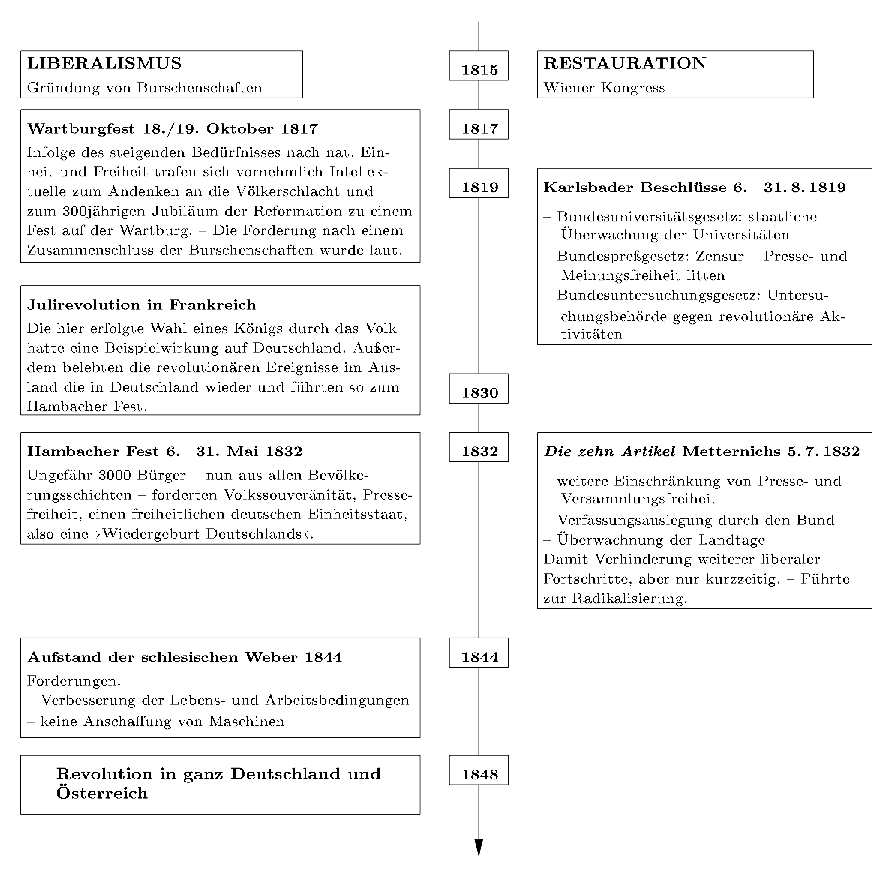
\includegraphics[width=\textwidth]{kampf-lib-rest.eps}
\caption{Das Ringen zwischen Liberalismus und Restauration}
\label{pic:kampf-lib-rest}
\end{figure}

Abbildung \ref{pic:kampf-lib-rest}\footnote{Die \ges{Zehn Artikel}
\Nam{Metternich, Klemens Wenzel Lothar von}{Metternichs} sind in
\cite{ZehnArt} zu finden, weitere Literatur in
\cite[106]{braunesGeschichts}. Die Quellen zu den übrigen Ereignissen
sind mir nicht bekannt.} zeigt die wichtigsten Ereignisse auf dem Weg
zur Revolution von 1848. Man erkennt, dass die Intensität von
antirestaurativen und restaurativen Maßnahmen immer weiter zunahm.
Weiter befeuert wurde die entwicklung durch die sich in Folge der
Industriellen Revolution verschärfenden soziale Lage.

%%%%%%%%%%%%%%%%%%%%%%%%%%%%%%%%%%%%%%%%%%%%%%%%%%%%%%%%%%%%%%%%%%%%%%

\subsection{Ursachenfeld}

\renewcommand*{\arraystretch}{1.5}
\newcolumntype{Y}{>{\setlength{\hsize}{0.55\hsize}\raggedleft}X}
\newcolumntype{Z}{>{\setlength{\hsize}{0.45\hsize}\raggedright}X}
\begin{tabularx}{\textwidth}{Y@{\quad$\lightning$\quad}Z}
restaurative Bewegung   & liberale Bewegung     \\
Absolutismus            & Aufklärung            \\
Industrielle Revolution -- Reichtum
                        & soziale Mißstände -- Armut    \\
territorialstaatlicher Absolutismus
                        & Einheitsbestrebungen
\end{tabularx}

%%%%%%%%%%%%%%%%%%%%%%%%%%%%%%%%%%%%%%%%%%%%%%%%%%%%%%%%%%%%%%%%%%%%%%

\subsection{Anlass}

Begünstigt durch die \dat{Krisenjahre 1847/48} in Frankreich mit
Missernten und Hungerunruhen kam es dort zur
\emph{Februarrevolution}\index{Februarrevolution}. Die Ereignisse in
Frankreich nahm man sich dann in Deutschland zum Vorbild und begann
die Revolution, die schon lange auf ihren Ausbruch gewartet hatte.
\mar{Germania und Bedeutung/Entwicklung von Symbolen.}

%%%%%%%%%%%%%%%%%%%%%%%%%%%%%%%%%%%%%%%%%%%%%%%%%%%%%%%%%%%%%%%%%%%%%%

\subsection{Verlauf}

\begin{figure}
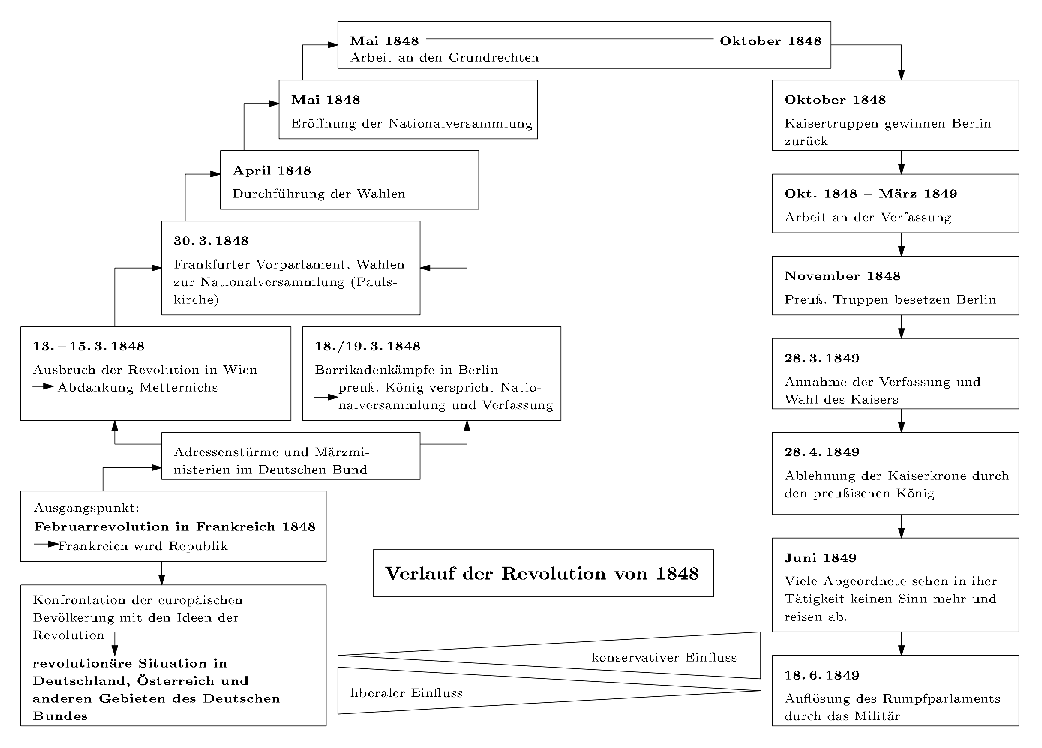
\includegraphics[height=\textwidth, angle=90]{verlauf-rev.eps}
\caption{Verlauf der Revolution von 1848}
\label{pic:verlauf-rev}
\end{figure}

Abbildung \ref{pic:verlauf-rev} bietet einen Überblick über den
Verlauf der Revolution. Diesen kann man in drei Etappen einteilen:
\mar{Richtige Benennung der Phasen?}

Die erste Phase war von kämpferischen Handlungen geprägt. Mit dem
Zusammentritt des \emph{Frankfurter Vorparlaments}
\index{Vorparlament!Frankfurt} begann eine Phase der Machtfestigung.
Der Niedergang setzte in der sehr langen Zeit der \emph{Arbeit an den
Grundrechten} ein. Diese Verzögerung der Vorgänge war nämlich einer
der Gründe für das Scheitern der Revolution: Durch die Uneinigkeit und
die fehlende parlamentarische Erfahrung, dauerte die Komprmissfindung
sehr lange. Das entstehende Machtvakuum nutzten die restaurativen
Kräfte für die Reaktion.

%%%%%%%%%%%%%%%%%%%%%%%%%%%%%%%%%%%%%%%%%%%%%%%%%%%%%%%%%%%%%%%%%%%%%%

\subsection{Verfassungsarbeit}

\begin{aufgabe}
Erläutern Sie die wesentlichen Aufgaben, die die
Paulskirchenversammlung zu lösen hatten und bilanzieren Sie die
jeweilige Lösung! 
\end{aufgabe}

\subsubsection{Parlament}

Das Parlament tagte in der runden
\Ort{Paulskirche!Frankfurt}{Frankfurter Paulskirche}\index{Frankfurt}.
Die 812 Männer unter dem Vorsitz des Liberalen \Nam{Gagern, Heinrich
von}{Heinrich von Gagern} waren hauptsächlich Bildungsbürger und
keinerlei Arbeiter. Man nannte die Versammlung daher auch
\jar{Parlament der Intellektuellen}.


\subsubsection{Grundrechte}
\index{Grundrechte}

Der erste Schwerpunkt der zukünftigten Verfassung für Deutschland
waren die Grundrechte. Auf Basis der Forderungen der Liberalen wurde
so ein umfangreicher Grundrechtskatalog beschlossen und im
\ort{Dezember 1848 angenommen}.


\subsubsection{Grenzen}

Eine sehr umstrittene Frage, die die Verhandlungen stark in die Länge
zog waren auch die zukünftigen Grenzen Deutschlands. Die
\emph{Großdeutsche Lösung} \index{Großdeutsche Lösung} sah neben den
deutschen Ländern die Einbeziehung der deutschsprachigen Teile
Österreichs vor. Diese wurde von vielen als die beste Variante
angesehen.

Österreich wollte jedoch sein gesamtes Staatsgebiet
einbringen, um als Gegengewicht zu Preußen auftreten zu können. Die
sogenannte \emph{Großösterreichische Lösung}
\index{Großösterreichische Lösung} war jedoch auch nicht möglich, da
man ein \emph{Deutsches} Reich wollte.

So fand man schließlich den Kompriss, Österreich ganz auszuschließen,
indem man zur \emph{Kleindeutschen Lösung} \index{Kleindeutschen
Lösung} gelangte.


\subsubsection{Staat}

Auch der \emph{Staatsaufbau} war Gegenstand langer Diskussionen zwischen
Demokraten, die eine Republik wollten und Liberalen, die eine
konstitutionelle Monarchie befürworteten. Das Ergebnis war das
System, welches Abbildung \ref{pic:verf-paulsk}\mar{Scan aus braunem
Geschichtsbuch S. 128 einfügen.} zeigt. \mar{Kriterien für
Verfassungsbewertung: Machtballungen, Rolle des Volkes, Verhältnis der
Organe} Es fallen dabei besonders die weitgreifenden Befugnisse des
Kaisers, die nicht mit dem Prinzip der Gewaltenteilung zu vereinbaren
sind, die freien Gerichte und der ausgeprägte Föderalismus auf.

Das Paulskirchenparlament musste auch die Entscheidung über das
künftige \emph{Staatsoberhaupt} fällen. Man wählte den Preußenkönig
\nam{Friedrich Wilhelm \Rm{4}}. Dieser lehnte allerdings ab, da er die
Krone nur \jar{aus den Händen eines deutschen Fürsten} empfangen
wollte. Die Verfassung war damit gescheitert.

%%%%%%%%%%%%%%%%%%%%%%%%%%%%%%%%%%%%%%%%%%%%%%%%%%%%%%%%%%%%%%%%%%%%%%

\mar{Das nennt sich wohl Bilanz.}
\subsection{Leistungen und Grenzen}

\begin{aufgabe}
Erörtern Sie die Darstellung, indem Sie die Hauptaussagen zur Wertung
der Revolution herausarbeiten, begründen, warum die Revolution trotz
iher fortschrittlichen Ideen scheiterte und sich zum Begriff des
epochalen Einschnitts für das Jahr 1848 positionieren!
\end{aufgabe}

\mar{?}
\begin{itemize}
\item Wertung der Verfassung
\item Nachweis des fraktionellen Kompromisses 
\end{itemize}

\subsubsection[Gründe des Scheiterns]{Gründe des
Scheiterns\mycite[138\,--\,140]{braunesGeschichts}}

\begin{itemize}
\item keine Hauptstadt $\rightarrow$ Polyzentrismus (viele kleine
Revolutionsherde)
\item keine parlamentarischen Machtmittel (Geld, Truppen)
\item Furcht vor Weiterführung der Revolution in soziale Revolution
\item Macht der Einzelmonarchen
\item Uneinigkeit durch unterschiedliche Ziele (auch sozial)
\item Unterschätzung der konservativen Kräfte
\end{itemize}


\subsubsection[Bedeutung für die deutsche Geschichte]{Bedeutung für
die deutsche Geschichte\mycite[140/141]{braunesGeschichts}}

\begin{itemize}
\item zuerst starke Zurückdrängung der liberalen Bewegung
\item Bestehenbleiben des Verfassungsstaates (konstitutionelle
Monarchien) in den deutschen Ländern außer Österreich
\item Abschaffung der Zensur

\item keine weitere Infragestellung von
\begin{itemize}
\item Bauernbefreiung
\item Ende der adeligen Patrimonialgerichtsbarkeit
\item Ende der Sonderrechte des Adels
\end{itemize}

\item moderne Gewerbeordnung
\item Obrigkeit sieht Reformbedürftigkeit ein
\item neues politisches Bewusstsein -- \emph{Geburtsstunde der Parteien}
\index{Parteien!Geburtsstunde}
\item Verfassungs- und Grundrechtsidee
\end{itemize}

%%%%%%%%%%%%%%%%%%%%%%%%%%%%%%%%%%%%%%%%%%%%%%%%%%%%%%%%%%%%%%%%%%%%%%

\subsection{Von der \jar{Revolution von unten} zur \jar{Revolution von
oben}}
\index{Revolution!von unten}
\index{Revolution!von oben}

Bereits \dat{Ende 1848} oktroyierte \nam{Friedrich Wilhelm \Rm{4}} in
Preußen eine Verfassung und kam damit den liberalen Bestrebungen in
geringem Maße selbst nach, setzte aber auch eindeutig seine Politik
durch. -- Sie enthielt unter anderem folgende Bestimmungen:

\begin{itemize}
\item Pressefreiheit
\item Gleichheit vor dem Gesetz
\item Zweikammersystem -- \Ins{Herrenhaus!Preußen}{Herrenhaus} vom
König berufen, \Ins{Abgeordnetenhaus!Preußen}{Abgeordnetenhaus} von
der Bevölkerung gewählt
\item Dreiklassenwahlrecht \index{Dreiklassenwahlrecht!Preußen} bei
öffentlicher und indirekter Wahl
\item Gesetze bedürfen der Zustimmung beider Häuser
\end{itemize}

Im Gegensatz zu Preußen hob Österreich \dat{1851 seine Verfassung
wieder auf} und kehrte damit zum Absolutismus zurück.

Schon \dat{1850} vereinbarten beide Staaten die \dat{Wiederherstellung
des \Ins{Deutscher Bund}{Deutschen Bundes}}. Mit der
\dat{Wiedereröffnung des \Ins{Frankfurter Bundestages}{Frankfurter
Bundestages} am 12. Mai 1851} und mit der \dat{Aufhebung der
\ges{Grundrechte des deutschen Volkes} im August} hatte in Preußen die
Reaktion endgültig gesiegt.

Folgende zwei Auszüge spiegeln das Klima der damaligen Zeit wider: Das
erste aus dem ausklingenden Vormärz mit deutlich appellativem
Charakter, das zweite aus der anbrechenden Zeit des Biedermeier
\index{Biedermeier} zeugt von Resignation\footnote{Liest man den
vollständigen Text, offenbart sich ein etwas anderer Charakter, doch
im Unterricht wurde wieder einmal auf die Praktik der Verheimlichung
zurückgegriffen.}:

\poemtitle*{Männer aus dem Proletariat!\mycite{ProlMaen} (1848)}
\settowidth{\versewidth}{geprügelt und geplagt von den erbärmlichsten
Gendarmentröpfen,}

\begin{verse}[\versewidth]
Handwerksburschen, \\
die ihr am Bettelstabe Deutschland durchzieht, \\
geschunden von den jammervollsten Polizeischergen, \\
geprügelt und geplagt von den erbärmlichsten Gendarmentröpfen, \\
laßt Euch doch nicht länger mehr als Hunde behandeln, \\
steht auf, fletscht die Zähne \mbox{[\dots]}! 
\end{verse}

\poemtitle*{\Nam{Pfau, Ludwig}{Ludwig Pfau} (1821\,--\,1891):
Badisches Wiegenlied (1849)\mycite{PfauWiegenl}}
\settowidth{\versewidth}{Und wer nicht schläft in guter Ruh’,}

\begin{verse}[\versewidth]
Schlaf’, mein Kind, schlaf leis’, \\
Dort draußen geht der Preuß’, \\
Deinen Vater hat er umgebracht, \\
Deine Mutter hat er arm gemacht, \\
Und wer nicht schläft in guter Ruh’, \\
Dem drückt der Preuß’ die Augen zu. \\
Schlaf’, mein Kind, schlaf leis’, \\
Dort draußen geht der Preuß’, \\!

Schlaf’, mein Kind, schlaf leis’, \\
Dort draußen geht der Preuß’, \\
Der Preuß' hat eine blut’ge Hand, \\
Die streckt er über’s badische Land, \\
Und alle müssen stille sein \\
Als wie dein Vater unterm Stein \\
Schlaf’, mein Kind, schlaf leis’, \\
Dort draußen geht der Preuß’,  \\
\mbox{[\dots]} \\
\end{verse}

%%%%%%%%%%%%%%%%%%%%%%%%%%%%%%%%%%%%%%%%%%%%%%%%%%%%%%%%%%%%%%%%%%%%%%

\subsection{Bilanz der liberalen Bewegung}

\begin{itemize}
\item \emph{Altliberale} galten als Verlierer der Revolution und
bildeten weiter den Gegenpol zur konservativen Bewegung.

\item Durch Industrialisierung gestärktes Wirtschaftsbürgertum
(\emph{Bourgeoisie}\index{Bourgeoisie}) suchte nach Kompromissen mit
den Konservativen (\emph{Realpolitiker}\index{Realpolitiker}).

\item Die Regentschaft des preußischen Kronprinzen seit \dat{1858} und
seit 1861 Köngis \Nam{Wilhelm \Rm{1}} begründete eine \dat{\beg{Neue
Ära}} in Preußen.
\end{itemize}

Das neue Kabinett brachte allerdings eine Reihe von Problemen mit
sich: Das \ins{Herrenhaus}, welches vom Junkeradel \index{Junkeradel}
dominiert wurde, blockierte nämlich von nun an alle Neuerungen. So kam
es dann auch zu dem Konflikt zwischen Konservativen und Liberalen um
eine Heeresreform (Aufstockung), der sich zu einem Verfassungskonflikt
auswuchs. Die Liberalen der zweiten Kammer bewilligten nämlich nur
einen provisorischen Haushalt für \dat{1860/1861}, woraufhin die
Konservativen reagierten, indem sie das Mitspracherecht des Parlaments
in Militärangelegenheiten einschränkten und so das Budgetrecht
aushebelten. Infolgedessen spalteten sich die Linksliberalen von den
Altliberalen ab und gründeten zusammen mit den Demokraten \dat{1861
die \ins{Fortschrittspartei}}, die erste klassische Partei auf
deutschem Boden.

\endinput




\endinput

\part{Demokratie und Diktatur -- Anspruch und Wirklichkeit von
Gesellschaftsmodellen in der ersten Hälfte des 20. Jahrhunderts}
\label{prt:dem-dikt}

\chapter{Das Deutsche Reich 1919 bis 1933 -- Die Weimarer Republik}
\label{chp:weim-rep}
\index{Deutsches Reich!1919 bis 1933}
\index{Weimarer Republik}

\begin{aufgabe}
Erläutern Sie den Platz der Weimaerer Republik in der deutschen
Geschichte!

Weisen Sie diese Position an der Weimarer Verfassung nach!
\end{aufgabe}

\section{Der \ins{Vertrag von Versailles}}
\label{sec:vvv}
\index{Erster Weltkrieg}
\index{Friedensvertrag!Versailles}

Die Verhandlungen über den Friedensvertrag der Alliierten des Ersten
Weltkrieges mit Deutschland \ort{begannen im Januar 1919}
\ort{Versailles}. Die Bedingungen wurden am \dat{23. Juni 1919} an die
deutsche Delegation, die an den vorangehenden Zusammenkünften nicht
teilnehmen durfte, übergeben und am \dat{28. Juni} im Spiegelsaal
\index{Spiegelsaal} von Versailles unterzeichnet.

\subsection*{Gebietsregelungen}

\begin{itemize}
\item \ort{Elsaß-Lothringen} geht an Frankreich.
\item \ort{Westpreußen} geht an Polen.
\item Schaffung eines polnischen Korridors zur Ostsee
\item \ort{Danzig} wird freie Stadt; Polen erhält Sonderrechte im
Hafen von Danzig
\item Das \ort{Memelgebiet} geht an Litauen, später an die
Sowjetunion.
\item \ort{Eupen-Malmedy} geht an Belgien.
\item Das \ort{Saargebiet} wird dem \ins{Völkerbund} unterstellt.
\item Die \ins{Saargruben} gehen zur Ausbeutung 15 Jahre an
Frankreich.
\item Die deutschen Kolonien\index{Kolonien!deutsch} werden dem
Völkerbund unterstellt.
\end{itemize}

\noindent $\Longrightarrow$ Deutschland verliert 10\,\% seiner
Bevölkerung und 13\,\% seiner Fläche


\subsection*{Politische Regelungen}

\begin{itemize}
\item Verbot eines Zusammenschluss des Deutschen Reiches mit
Österreich (eigentlich durch den \ges{Vertrag von Saint
Germain}\Ort{Saint Germain}{}
\item Das Deutsche Reich erhält mit dem §\,231 die alleinige
Kriegsschuld und daraus abgeleitet die Pflicht zur Zahlung aller
Reparationen. \index{Kriegsschuldparagraph}\index{Reparationen!Erster
Weltkrieg} 
\end{itemize}


\subsection*{Militärische Regelungen}

\begin{itemize}
\item Reduzierung der deutschen Armee auf 100\,000 Mann, der Marine
auf 15\,000 Mann.
\item Verbot von Flugzeugen, Panzern, U-Booten und schweren
Kriegsschiffen
\item Auslieferung der Kriegsflotte
\item Verbot eines Generalstabes\index{Generalstab}
\item militärische Besetzung des linken \Ort{Rheinufer}{Rheinufers}
durch Frankreich, einige rechtsrheinische
Brückenköpfe\index{Rheinufer!Brückenköpfe} für 15 Jahre
\item Entmilitarisierung eines rheinischen Streifens
\end{itemize}


\subsection*{Wirtschaftliche Regelungen}

\begin{itemize}
\item durch die Gebietsabtrennungen betroffen: Bergbau,
Stahlindustrie, Hüttenwesen, Landwirtschaft
\item \dat{1921 Fixierung} der Reparationen auf 132 Milliarden
Reichsmark\index{Reparationen!Erster Weltkrieg}
\end{itemize}


\subsection*{Folgen in Deutschland}

\begin{itemize}
\item Austritt der \ins{DDP} aus der \ort{Weimarer Koalition}

\item Rücktritt des Ministerpräsidenten \Nam{Scheidemann,
Philipp!Rücktritt}{Scheidemann} und des Außenministers
\Nam{Brockdorff-Rantzau, Ulrich von!Rücktritt}{von Brockdorff-Rantzau}

\item gleichfalls Rücktritt des Reichswehrministers \Nam{Noske,
Gustav!Rücktritt}{Noske} (\ins{SPD}) und des verfassungstreuen Generals
und Chefs der \ins{Heeresleitung} \Nam{Reinhardt,
Walther!Rücktritt}{Reinhardt} -- Neubesetzung der Stellen durch den
\beg{Vernunftrepublikaner} \Nam{Gessler, Otto}{Gessler} (DDP) und den
Antirepublikaner General \Nam{Seeckt, Hans von}{von Seeckt}

\item Hohe Reparationszahlungen bremsen den Wiederaufbau und führen zu
Unzufriedenheit, Armut und Arbeitslosigkeit. Die übertriebenen
Ansprüche der Alliierten führen schließlich zum
\emph{Ruhrkampf}\index{Ruhrkampf} (siehe \ref{sec:krisj-1923}).
\end{itemize}



\endinput

\section{Parteien}
\mar{Siehe hierzu auch das Arbeitsblatt aus der Sekundarstufe \Rm{1}}

\subsection*{Republiksgründung}

Tabelle \ref{tab:vergl-part-weimrep} bietet eine Übersicht über die
Parteien, die bei der Gründung der Weimarer Republik bestimmend waren.
Dabei ist noch zu bemerken, dass nur SPD, DDP und Zentrum
staatstragende Parteien waren, alle Parteien eine Revision des
\ges{Vertrag von Versailles}{Vertrages von Versailles} anstrebten und
dass die DNVP den Wiedererwerb von Kolonien und die Erneuerung des
deutschen Kaisertums befürwortete.

%{
%\small
%\renewcommand{\arraystretch}{0.8}
%
%% Wir müssen doch mal wieder berechnen.
%\newlength{\frstcolwdth}
%\settowidth{\frstcolwdth}{\textit{Zentrum}}
%
%\newlength{\dumwdth}
%\setlength{\dumwdth}{\textwidth}
%\addtolength{\dumwdth}{-\frstcolwdth}
%\newlength{\othcolwdth}
%\setlength{\othcolwdth}{0.5\dumwdth}
%\addtolength{\othcolwdth}{-3\tabcolsep}
%
%\tablecaption{bla}
%\tablefirsthead{
%\toprule
%
%Partei &
%Politisches System &
%Wirtschaftliches System \\
%
%\midrule
%}
%
%\begin{supertabular*}{\textwidth}{cp{\othcolwdth}p{\othcolwdth}}
\begin{table}
\caption{Vergleich von Parteien der Weimarer Republik}
\label{tab:vergl-part-weimrep}

\renewcommand{\arraystretch}{0.8}
\footnotesize

\begin{tabularx}{\textwidth}{cXX}
\toprule

Partei &
Politisches System &
Wirtschaftliches System \\

\midrule

\Ins{DNVP, Deutschnationale Volkspartei}{DNVP} &
\vspace{-0.7em}
\begin{tablist}
\item überparteiliche (Hohenzollern-) Monarchie 
\item starke Exekutive
\item Mitwirkung des Parlaments bei der Gesetzgebung
\item Ständevertretung zusätzlich zur Volksvertretung
\end{tablist}
&
\vspace{-0.7em}
\begin{tablist}
\item Eigenwirtschaft und Privateigentum
\item Sozialisierung mit äußerster Vorsicht
\item Förderung eines starken Mittelstandes und der Landwirtschaft 
\end{tablist}
\\

\Ins{DVP, Deutsche Volkspartei}{DVP} &
\vspace{-0.7em}
\begin{tablist}
\item Monarchie
\item Verantwortliche Mitwirkung des Parlaments an der Regierung 
\end{tablist}
&
\vspace{-0.7em}
\begin{tablist}
\item Privatwirtschaft
\item keine Sozialisierung
\item Förderung der Landwirtschaft und des Mittelstandes 
\end{tablist}
\\

\Ins{DDP, Deutsche Demokratische Partei}{DDP} &
\vspace{-0.7em}
\begin{tablist}
\item demokratische Republik auf dem Boden der Weimarer Verfassung
\item liberaler und sozialer Rechtsstaat 
\end{tablist}
&
\vspace{-0.7em}
\begin{tablist}
\item Privatwirtschaft
\item gegen jegliche Vergesellschaftung
\item Schutz von Handwerk und Mittelstand 
\end{tablist}
\\

\Ins{Zentrum, Deutsche Zentrumspartei}{Zentrum} &
\vspace{-0.7em}
\begin{tablist}
\item demokratische Republik 
\item christliche Grundsätze
\item bürgerliche Freiheiten
\item soziale Gerechtigkeit
\end{tablist}
&
\vspace{-0.7em}
\begin{tablist}
\item Recht auf Privateigentum
\item Förderung des Genossenschaftswesens
\item Verstaatlichung nur gegen Entschädigung
\item Schutz des Mittelstands und des Bauernstands
\end{tablist}
\\

\Ins{SPD, Sozialdemokratische Partei Deutschlands!Weimarer
Republik}{SPD} &
\vspace{-0.7em}
\begin{tablist}
\item demokratische Republik
\item Demokratisierung des Staates und der Gesellschaft
\item Erneuerung der Gesellschaft
\item sozialistisches Gemeinwesen
\end{tablist}
&
\vspace{-0.77em}
\begin{tablist}
\item Überwindung des kapitalistischen Systems
\item Förderung des gemeinwirtschaftlichen Gedankens
\item Genossenschaftswesen
\item Überführung der Konzerne in die GemeInschaft
\item Verstaatlichung von Grund und Boden
\end{tablist} 
\\

\Ins{KPD, Kommunistische Partei Deutschlands!Weimarer Republik}{KPD} &
\vspace{-0.7em}
\begin{tablist}
\item Errichtung einer sozialistischen Gesellschaftsordnung
\item revolutionäre Umgestaltung von Staat, Gesellschaft und
Wirtschaft
\item Übernahme der staatlichen Funktionen durch Arbeiterräte 
(Räterepublik)
\end{tablist}
&
\vspace{-0.7em}
\begin{tablist}
\item Enteignung von Banken, Industrie --
Vergesellschaftung der Industrie und des Kapitals
\item Enteignung von Großgrundbesitz -- Bildung sozialistischer
landwirtschaftlicher Genossenschaften
\end{tablist}
\\

\bottomrule
\end{tabularx}
\end{table}
%\end{supertabular*}
%}

\subsection*{Rechtsextremistische Strömung}
\index{Antimarxismus}
\index{Antiliberalismus}
\index{Antisemitismus}
\index{Jugendkult}
\index{Führerkult}
\index{Nationalsozialismus!Weimarer Republik}

Zu Anfang der Weimarer Republik noch von geringer Bedeutung, nahm die
Bedeutung der rechtsextremistische Strömung, politisch vor allem durch
die \ins{NSDAP, Nationalsozialistische Deutsche Arbeiterpartei}{NSDAP}
verkörpert, rasch zu. Sie war charakterisiert durch ideologische
Prägung mit \emph{Antimarxismus}, \emph{Antiliberalismus} und
\emph{Antisemitismus}, Betonung von Werten wie Einigkeit und Treue,
Militarismus als Lebenform und völkisch mystifizierten Jugend- und
Führerkult.

Mit den Konservativen gemein hatten sie die starke Ablehnung der
Weimarer Republik (\jar{Republik der Novemberverbrecher}) und die
Forderung nach einem starken Staat. Sie zeichneten sich aber durch
größere Radikalität, die auch vor Gewalttaten bis hin zu Morden nicht
zurückschreckte, Bildung einer \jar{kriegerischen Elite} sowie das
Ziel eines \jar{nationalen Sozialismus} aus.

\endinput

\section[Revisions- und Erfüllungspolitik -- Die Rolle politischer
Handlungsträger]{Revisions- und Erfüllungspolitik -- Die Rolle
politischer
Handlungsträger\mycite[339\,--\,348]{braunesGeschichts}\,\mycite[356\,--\,360]{gelbesGeschichts}\,\mycite[26\,f.,
32\,f.]{IzpBWeimRep}}
\label{sec:rev-erf-pol}
\index{Revisionspolitik}
\index{Erfüllungspolitik}

\subsection*{Vertrag von Rapallo}

Nach dem Ersten Weltkrieg standen die Russische Sozialistische
Föderative Sowjetrepublik (RSFSR) und das Deutsche Reich
wirtschaftlich und politisch isoliert da. -- Erstere wegen der
westlichen Angst vor dem Kommunismus, letzteres wegen seiner Rolle im
Krieg. In dieser Situation beschlossen sie \dat{1922 im \ges{Vertrag
von Rapallo}} gegenseitigen \Ort{}{Rapallo}
\emph{Reparationsverzicht}\index{Reparationen!Rapallo}, Aufnahme
\emph{diplomatischer Beziehungen} und
\emph{Meistbegünstigung}\index{Meistbegünstigung!Rapallo} in den
wirtschaftlichen Beziehungen. Gleichzeitig wurde der \ges{Vertrag von
Versailles} unterwandert, indem die Hilfe deutscher Experten bei der
Entwicklung russischen schweren Kriegsgeräts vereinbart wurde, was mit
der Möglichkeit der Übung deutscher Militärs am Material einherging.

Der Vertrag von Rapallo verärgerte also durch die Veränderung der
Situation in Osteuropa Großbritannien und Frankreich und übte
gleichzeitig Druck auf diese aus. Denn nun waren Polen und die
Tschechoslowakei, die eine Schutzgürtel gegen den Kommunismus bilden
sollten, in eine Zweifrontenlage geraten. Es war nun die Zeit für
Deutschland gekommen, außenpolitisch aktiv zu werden.

%%%%%%%%%%%%%%%%%%%%%%%%%%%%%%%%%%%%%%%%%%%%%%%%%%%%%%%%%%%%%%%%%%%%%%

\subsection*{Ära Stresemann}
\index{Ära Stresemann}

\nam{Stresemann, Gustav}{Gustav Stresemann} war von August bis
November 1923 Reichskanzler und danach bis zum seinem Tode im Jahre
1929 Außenminister in der Weimarer Republik. Seine Rolle in der
Politik der damaligen Zeit war bestimmen, weswegen man von der
\jar{Ära Stresemann} spricht, sodass sein Ableben zu einem Machtvakuum
führte, das in die Präsidialkabinette (siehe \ref{sec:praes-kab})
mündete.

Seine Ziele war das Wiedererstarken Deutschlands auf Grundlage der
Lösung des Reparationsproblems und der Revision des \Ges{Vertrag von
Versailles}{Vertrags von Versailles}, die mit der Korrektur der
Ostgrenzen, der Vereinigung mit Deutsch-Österreich und dem Schutz der
Auslandsdeutschen einhergingen. Er war also eindeutig ein
Revisionspolitiker, sah aber anders als viele andere Gegner des
Vertrags von Versailles die einzige Möglichkeit der Erreichung seiner
Ziele in der Friedenssicherung durch die Aussöhnung mit Frankreich und
den Eintritt in den \ins{Völkerbund}.\mycite{StresWil}

\subsubsection{Dawes-Plan}
\index{Dawes-Plan}

Da das Deutsche Reich offensichtlich Schwierigkeiten hatte
(\emph{Ruhrkampf}\index{Ruhrkampf}, siehe \ref{sec:krisj-1923}),
seinen Reparationspflichten nachzukommen, legte der US-amerikanische
Bankier \nam{Dawes, Charles}{Charles Dawes} ein Programm vor, dass
einen angemessenen Zahlungsplan sowie die Möglichkeit der
Kreditaufnahme vorsah. Dabei wollten die USA gleichfalls Absatzmärkte
schaffen -- das Geld aus dem Kredit über 800 Millionen Reichsmark
musste in den USA ausgegeben werden -- und den internationalen Markt
stabilisieren, um die Gefahr der Ausbreitung des Kommunismus mindern.

\dat{1924 unterzeichneten} die beteiligten Mächte auf der
\ins{Londoner Konferenz}\Ort{London}{} das betreffende Abkommen,
welches zugleich zur wirtschaftlichen und politischen internationalen
Integration des Deutschen Reiches (\emph{Eintrittskarte} nach Europa)
und damit zur Entspannung in Europa führte. Die ökonomische
Stabilisierung in Deutschlands war auch Ursache für die Scheinblüte der
\jar{Goldenen Zwanziger}.\index{Goldene Zwanziger}\index{Scheinblüte}
Allerdings war das Deutsche Reich nun finanziell von den USA abhängig.
Daher schlug die \ins{Weltwirtschaftskrise} 1929 hier besonders hart
zu.


\subsubsection{Verträge von Locarno}

Die \ges{Verträge von Locarno}\Ort{Locarno}{} wurden \dat{1925} auf
einer Konferenz von Politikern Belgiens, Deutschlands, Frankreichs,
Großbritanniens, Italiens, Polens und der Tschechoslowakei
\dat{geschlossen} und errichteten den Prinzipien der \Nam{Stresemann,
Gustav}{stresemann}schen Außenpolitik folgend ein europäisches
Sicherheitssystem.

\paragraph{Inhalte} Mit dem \ges{Westpakt} verzichteten Belgien, das
Deutsche Reich und Frankreich auf eine gewaltsame Veränderung der
gemeinsamen Grenzen.  Letzteres schloss damit auch Ansprüche auf
\ort{Eupen-Malmedy} und \ort{Elsaß-Lothringen}. Die Einhaltung dieses
Vertrages überwachten Großbritannien und Italien als Garantiemächte.

Der \ges{Rheinpakt} vereinbarte den schrittweisen Abzug der
französischen Truppen aus dem \ort{Rheinland}.

Stresemann wollte ausdrücklich keine Garantie der deutschn Ostgrenze.
Der \ges{Ostpakt} war deshalb lediglich ein Schiedsvertrag mit Polen,
der eine gewaltsame Veränderung der Grenze ausschloss.

\paragraph{Folgen} International bedeuteten die Verträge einen großen
weiteren Schritt zur Rehabilitation des Deutschen Reiches und beendete
seine außenpolitische Isolation endgültig. Sie ermöglichten nämlich
dessen \dat{Aufnahme in den \ins{Völkerbund} 1926} -- ein lange
verfolgtes Ziel Stresemanns. Hier war das Deutsche Reich ein
gleichberechtigter Partner zwischen den anderen Großmächten und hier
konnte der Außenminister der Welt seine Anliegen, insbesondere
bezüglich der Auslandsdeutschen\index{Auslandsdeutsche} vorzutragen.

National wurden die Verträge von rechts und links angefeindet. Jene
beschimpften das Vorgehen Stresemanns und der anderen Beteiligten als
\emph{Erfüllungspolitik}\index{Erfüllungspolitik}, als Schwäche und
\jar{Unehre} des Deutschen Reiches. Diese wetterten ob der angeblichen
\jar{imperialistischen} und \jar{antikommunistischen} Bestrebungen. So
oder so wurden die Verträge von Locarno eine Plattform für Propaganda
gegen die Weimarer Republik.


\subsubsection{Berliner Vertrag}

Wegen der Einbindung des Deutschen Reiches in das westliche
Staatensystem infolge der \ges{Verträge von Locarno}\Ort{Locarno}{}
befürchtete man in der UdSSR, dass sich jenes von den Festlegungen des
\Ges{Vertrag von Rapallo}{Vertrages von Rapallo}\Ort{Rapallo}{}
entfernen könnte.  Deshalb schlossen beide Staaten \dat{1926 den
\ges{Berliner Vertrag}}, indem sie sich die gegenseitige Neutralität
für den Fall eines Krieges zusicherten. Laut \cite[33]{IzpBWeimRep}
bedeutete das insbesondere, dass das Deutsche Reich den Durchmarsch
französischer Truppen bei einem Krieg zwischen der Sowjetunion und
Polen untersagen würde.


\subsubsection{Briand-Kellog-Pakt}

\dat{1928 initiierten} der französische Außenminister \Nam{Briand,
Aristide}{Aristide Briand}, der schon maßgeblich zum Zustandekommen
der \ges{Verträge von Locarno}\Ort{Locarno}{} beigetragen hatte, und
\Nam{Kellogg, Frank Billings}{Frank Billings Kellogg} einen
Vertrag zur Ächtung des Krieges, den \ges{Briand-Kellogg-Pakt}. Unter
den anfänglich 15 Unterzeichnerstaaten befand sich auch das Deutsche
Reich. Nach und nach traten dann weitere Staaten bei, sodass es
schließlich circa 60 wahren.


\subsubsection{Young-Plan}

Die nach wie vor nich gelöste Frage der deutschen Reparationen trieb
die Politiker weiter um, bis schließlich \dat{1929} ein unter der
Leitung des amerikanischen Wirtschaftsfachmann \Nam{Young, Owen}{Owen
Young} ausgearbeiteter Plan \ges{Young-Plan}{} \dat{verabschiedet}
wurde, der folgende Regelungen enthielt:

\begin{enumerate}
\item Die Gesamtsumme der Reparationen wird auf 114 Milliarden
Goldmark festgesetzt.
\item Deutschland soll 59 Jahre lang zahlen.
\item Die Höhe der Raten steigt in den ersten 37 Jahren von 1,7 auf
2,1 Milliarden Goldmark.
\item Ausländische Wirtschaftskontrollen in Deutschland entfallen.
\item Die alliierten Besatzungstruppen werden bereits 1930, also fünf
Jahre früher, aus Deutschland (\ort{Rheinland}) abgezogen.
\end{enumerate}

\mar{Tauch Lausanne irgendwann mit auf?}

\subsection*{Bilanz}\mar{Nur der Form halber.}

\begin{itemize}
\item Deutschland ist rehabilitiert, aber noch nicht vollständig
souverän. 
\item Der \ges{Vertrag von Versailles} (Kriegsschuldparagraph!) ist
nicht revidiert.
\item Die Verträge, insbesondere die von Locarno, bieten eine
Propagandaplattform für Republikfeinde.
\item Der \dat{Tod Stresemanns 1929} hinterlässt ein Machvakuum,
infolgedessen die Zeit der Präsidialkabinette beginnt.
\end{itemize}


\endinput

\section{Das Krisenjahr 1923}
\label{sec:krisj-1923}

Siehe hierzu das Arbeitsblatt, von dessen Autorinnen ich \Nam{Barth,
Lina}{Lina Barth} ich noch im Gedächtnis habe.

\endinput

\section{Inflation}
\label{sec:soz-veraend}
\index{Inflation!Weimarer Republik}
\index{Hyperinflation}

Während des Krieges hatte die Inflationsrate im Deutschen Reich zu
steigen begonnen. Diese Tendenz kuliminierte \dat{1923}, als die
schleichende Inflation zur galoppierenden und schließlich zur
\dat{Hyperinflation} wurde. Nun erst wurde das Problem mit der
\dat{Währungsreform vom 15. November 1923}, die die \ins{Rentenmark}
einführte, wobei eine Rentenmark den Wert von 1\,000\,000\,000\,000 (1
Bio.) Papiermark und 4,2 Dollar den Wert einer Rentenmark
hatte.\mycite[28]{IzpBWeimRep}

\subsection*{Folgen}

\subsubsection{Wirtschaft}

\begin{itemize}
\item materielle Verluste
\item Vermögensumschichtung
\item Löhne auf Vorkriegsnieveau
\item Vernichtung von Geldvermögen
\item Konzentrationsprozesse -- Konternbildung 
\end{itemize}


\subsubsection{Bevölkerung}

\begin{itemize}
\item Abhängigkeit von der Armenfürsorge
\item Zerfall des klassischen Bildungsbürgertums als Träger der
Gesellschaft durch finanzielle Entmachtung
\item Sachwertbesitzer werden zu Geldwertbesitzern
\item materielle und damit seelische Not
\item soziale Schichtung (Klassengesellschaft im Übergang)\mar{?}
\item Neuerungen im sozialen Bereich (bspw. Sozialverischerung) 
\item hohe Arbeitslosenrate
\end{itemize}


\subsubsection{Politik}

Die Inflation wirkte sich auf die Politik insofern aus, als die
Radikalisierung, das heißt die Entfernung von den Parteien der Mitte,
vorangetrieben wurde. Dies zeigte sich in den Wahlen von 1924.


\subsection*{Bilanz}

\subsubsection{Gewinner}

\begin{itemize}
\item Staat -- Lösung des Schuldenproblems
\item Sachwertbesitzer
\item Unternehmer -- Kredite aus getätigten Modernisierungs- oder
Erweiterungsinvestitionen konnten mühelos getilgt werden. 
\end{itemize}

\subsubsection{Verlierer}

\begin{itemize}
\item Staat -- Die Menschen schoben die Schuld am Elend den
staatstragenen Parteien zu und wendeten sich an die Radikalen.
\item Mittelschicht, Stadtbewohner -- Verlust von Erspartem
(Alterssicherung), großen Einkommensverluste vor der Reform
\item Ausland -- Gesamtverluste auf deutschen Bankguthaben und
Wertpapierbeständen von circa 15 Milliarden Goldmark
\end{itemize}

\endinput

\section{Jugend}

\ges{Dawes-Plan} (siehe \ref{sec:rev-erf-pol}) und
Inflation\index{Inflation} (siehe \ref{sec:soz-veraend})
bewirkten

\begin{itemize}
\item sozial:

\begin{itemize}
\item Jugendarbeitslosigkeit -- Jugendliche fallen den Familien länger
zur Last
\item Verbitterung durch fehlende Freizeitangebote:

\begin{itemize}
\item verstärkte Neigung zu Protest- und Gewalttaten 
\item Verlust der Autorität der Familie
\item Jugendkriminalität
\end{itemize}

\item \jar{vergreiste Republik} -- Die Jugend fühlt sich um Lebens-
und Karrierechancen betrogen.
\end{itemize}

\item politisch:

\begin{itemize}
\item hohe Anfälligkeit gegenüber radikalen Ideologien und
Gruppierungen
\item studentische Wahlen Ender der 1920er\mar{?} -- hoher
Stimmenanteil für völkisch-nationalistische Gruppen
\end{itemize}
\end{itemize}

Insgesamt fallen also auf:

\begin{itemize}
\item antidemokratisches Denken
\item starker Widerwille gegen westlich-liberale Weltreaktion \mar{?}
-- Radikalismus nach links und rechts
\item glauben an Ideen, statt an aufgeklärten Verstand
\end{itemize}

\endinput

\section{Auswirkungen der Weltwirtschaftskrise auf Deutschland}
\index{Weltwirtschaftskrise}
\index{Börsenkrach}
\index{Schwarzer Freitag}

Der Konjunkturrückgang in den USA führte dort am \dat{25. Oktober
1929}, dem sogenannten \emph{Schwarzen Freitag}, schließlich zum
\dat{Börsenkrach}. Infolgedessen zogen die USA die kurzfristigen
Kredite aus Deutschland (und den anderen europäischen Staaten) ab, was
dort zu Geldverknappung und Zahlungsschwierigkeiten bei den Banken
führte. Um einen vollständigen Zusammenbruch zu verhindern, trat der
Staat zwar mit Geldreserven ein. Doch der Kaufkraftverlust führte zur
Überproduktion, welche die Betriebe zu Produktionseinschränkungen
veranlasste. Diese mündeten in Massenentlassungen, sodass schließlich
die Wirtschaft völlig am Boden war. 

\endinput

\section{Präsidialkabinette}
\label{sec:praes-kab}

Siehe hierzu das altbewährte Schema und die ebenso altbewährte
Tabelle.

\endinput

\section{Gründe des Scheiterns der Weimarer Republik -- Eine Bilanz}

\begin{aufgabe}
Erarbeiten Sie aus der Quelle die Ursachen des Scheiterns der Weimarer
Republik aus Sicht des Autors!

Erläutern Sie an zwei selbst gewählten historischen Beispielen deren
destruktive Wirkung auf die Weimarer Republik!

Bewerten Sie den Stellenwert der gewählten Beispiele im Gesamtgefüge!
\end{aufgabe}

Siehe hierzu das gleichnamige Arbeitsblatt.

\endinput


\chapter{Das Deutsche Reich 1933 bis 1945}
\label{chp:drittes-reich}
\index{Deutsches Reich!1933 bis 1945}
\index{Drittes Reich}

\section{Grundlagen}

\subsection[Ideologie des
Nationalsozialismus]{Ideologie\mycite[386\,--\,389]{gelbesGeschichts}
des Nationalsozialismus}
\index{Ideologie!Nationalsozialismus}
\index{Blut und Boden}
\index{Chauvinismus}
\index{Militarismus}

{
\small
\newlength{\antsemlength}
\settowidth{\antsemlength}{Antisemitismus}

\newcommand*{\nodebox}[1]{\parbox{\antsemlength}{#1}}

\begin{bundle}{\textbf{Sozialdarwinismus}}
  \chunk[\footnotesize Blut]{\nodebox{Rassismus\newline Antisemitismus}}
  \chunk[\footnotesize Boden]{
    \begin{bundle}{\nodebox{Nationalismus\newline \beg{Chauvinismus}}}
      \chunk{Führerprinzip}
      \chunk{Lebensraumtheorie}
      \chunk{Volksgemeinschaft}
      \chunk{Militarismus}
    \end{bundle}
  }
\end{bundle}
}


\subsubsection[Rassismus und Antisemitismus]{Rassismus und
Antisemitismus (siehe auch \ref{sec:aussch-gegner})}
\index{Rassismus}
\index{Antisemitismus}
\index{Rassenantisemitismus}
\index{Rassenlehre}
\index{Arier}

\begin{itemize}
\item Biologisierung des Sozialen -- Bestimmung des Verhaltens durch
Gene
\begin{itemize}
\item Höher-/Minderwertigkeit von Rassen: \jar{arische Rasse}
(nordisch), \jar{Kuli- und Fellachenrassen} (afrikanisch und
asiatisch), Juden
\item Schwache und Bedürftige schwächen mit ihren \jar{Erbanlagen} das
\jar{deutsche Volk}
\end{itemize}

\item Antisemitismus nicht mehr aus sozialen und religiösen Gründen,
sondern Rassenantisemitismus -- \jar{jüdische Rasse} als
\jar{minderwertig} und \jar{schmarotzend}

\item Rassismus und Antisemitismus werden zum Mittelpunkt des
politischen Denkens
\end{itemize}


\subsubsection{Führerkult}
\index{Führer}
\index{Führerkult}
\index{Führerprinzip}

\begin{itemize}
\item bedingungslose Unterwerfung des Einzelnen unter die Ziele des
Staates
\item Ausschluss von Opposition
\item Vereinigung aller Gewalten im \jar{Führer} 
\end{itemize}


\subsubsection{Lebensraumtheorie/-politik}
\index{Lebensraumtheorie}
\index{Lebensraumpolitik}

\begin{itemize}
\item \jar{germanische Rasse} hat Herrschaftsanspruch
\item Ausdehnung in Richtung Osten
\item Unterwerfung der \jar{Untermenschen}
\end{itemize}


\subsubsection{Volksgemeinschaftsideologie}
\index{Volksgemeinschaft}

\begin{itemize}
\item Wiedergeburt des deutschen Reiches
\item Verbot aller Parteien außer der NSDAP
\item Zusammenfassung aller politischen und sozialen Gruppen zu einer
\jar{Volksgemeinschaft}, Unterordnung und den Willen des \jar{Führers}
-- Überwindung sozialer, beruflicher und ideologischer Unterschiede
\end{itemize}


\subsection{Sicht des Großteils der Bevölkerung auf die Weimarer
Republik um 1933}

\begin{figure}
\centering
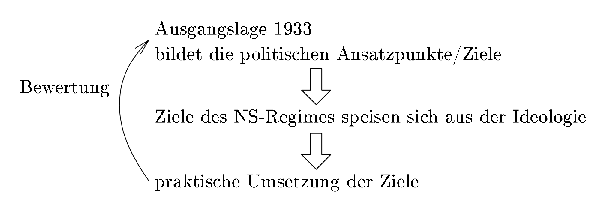
\includegraphics{bew-mass-ns.eps}
\caption{Bewertung der Wirksamkeit der Maßnahmen des NS-Regimes}
\label{pic:bew-mass-ns}
\end{figure}

Der Zustand der Weimarer Republik zu Anfang des Jahres 1933 bildete
die Ausgangslage für die Nationalsozialisten. Um deren Maßnahmen
hinsichtlich ihrer Wirksamkeit zu bewerten ist es zweckmäßig, zu
überprüfen, inwieweit sie Veränderungen gegenüber jener Ausgangslage
herbeiführten (siehe Abbildung \ref{pic:bew-mass-ns}) und wie die
Bevölkerung reagierte.

\begin{itemize}
\item wirtschaftliche Krise -- hohe Arbeitslosigkeit und Armut

\item Verhinderung wirtschaftlicher Erholung durch unfähige Demokraten
(\Nam{Brüning, Heinrich}{Brüning}s Deflationspolitik)

\item Wunsch nach
\begin{itemize}
\item Revision des \Ges{Vertrag von Versailles}{Vertrags von Versailles}

\item großdeutschem Reich -- Deutschland als militärische und
politische Großmacht

\item Verringerung der Arbeitslosigkeit
\end{itemize} 
\end{itemize}

%%%%%%%%%%%%%%%%%%%%%%%%%%%%%%%%%%%%%%%%%%%%%%%%%%%%%%%%%%%%%%%%%%%%%%

\subsection{Ziele der nationalsozialistischen Politik}

Aus dem vorhergehenden Abschnitt ergaben sich folgende Ansatzpunkte
für die Nationalsozialisten, um sich die Unterstützung der Bevölkerung
zu sichern:

\begin{itemize}
\item Wirtschaft
\begin{itemize}
\item Autarkie
\item Bekämpfung der Arbeitslosigkeit 
\end{itemize} 

\item Innenpolitik
\begin{itemize}
\item Ausschaltung der legalen Machtbasis
\item Zentralgewalt
\item Ausgrenzung der Nichtarier
\end{itemize}

\item Außenpolitik
\begin{itemize}
\item Revision des \Ges{Vertrag von Versailles}{Vertrags von Versailles}
\item Osterweiterung
\end{itemize}
\end{itemize}

Diese Ziele leiteten sich ebenfalls aus der Ideologie des
Nationalsozialismus ab, welche sich wiederum im \Ges{NSDAP,
Nationalsozialistische Deutsche Arbeiterpartei!Programm}{Programm der
NSDAP}\mycite{ProgNSDAP} niederschlug.

\endinput

\section{Innenpolitik}

\subsection*{NSDAP im Kabinett Hitler ab 30. Januar 1933}

\begin{description}
\item[\Nam{Hitler, Adolf}{Hitler}] Reichskanzler: Leitung der
Kabinettssitzungen, Bestimmung der politischen Richtlinien 

\item[\Nam{Frick, Wilhelm}{Frick}] Innenminister: verantwortlich für
die innere Sicherheit -- Vorbereitung und Durchführung von Gesetzen
und Notverordnungen (Zeitungs-, Versammlungs, Parteiverbot)

\item[\Nam{Göring, Hermann}{Göring}] Minister ohne Geschäftsbereich:
erhält das \ins{Reichskommissariat für das preußische
Innenministerium} -- Kontrolle über die preußische Polizei
\end{description}

%%%%%%%%%%%%%%%%%%%%%%%%%%%%%%%%%%%%%%%%%%%%%%%%%%%%%%%%%%%%%%%%%%%%%%

\subsection*[Maßnahmen Februar bis März 1933]{Maßnahmen Februar bis
März 1933\mycite[402]{gelbesGeschichts}}

Am \dat{1. Februar 1933} ließ \Nam{Hitler, Adolf}{Hitler} durch
\Nam{Hindenburg, Paul von}{Hindenburg} den \dat{Reichstag auflösen}.
Er begründete dieses Handeln damit, dass die Bildung einer
arbeitsfähigen Mehrheit im Parlament nicht möglich sei. Vorher hatte
er seine Scheinverhandlungen mit \Nam{Kaas, Ludwig}{Ludwig Kaas}
(Zentrum) scheitern lassen.

Danach begann der staatliche Terror, der die Ausschaltung
beziehungsweise Vernichtung der \jar{inneren} oder auch
\jar{Reichsfeinde} (Juden, gegnerische Politiker -- hauptsächlich KPD
und SPD) zum Ziele hatte. Gesetzliche Grundlage dafür war die
\dat{\ges{Reichstagsbrandverordnung} vom 28. Februar}. Diese führte
die \beg{Schutzhaft} ein; außerdem entstanden erste
Konzentrationslager.

Außerdem beeinflusste man im Hinblick auf die für \dat{März}
angesetzten \dat{Wahlen} die Bevölkerung durch Forcierung
propagandistischer Maßnahmen.

%%%%%%%%%%%%%%%%%%%%%%%%%%%%%%%%%%%%%%%%%%%%%%%%%%%%%%%%%%%%%%%%%%%%%%

\subsection*[Maßnahmen März 1933 bis August 1934]{Maßnahmen März 1933
bis August 1934\mycite[392\,--\,398]{gelbesGeschichts}}

Siehe dazu das Arbeitsblatt mit der Übersicht.

\endinput

\section{Wirtschaft}

\begin{aufgabe}
zu eingebunden -- siehe Hefter
\end{aufgabe}

\begin{itemize}
\item \jar{Rettung} der Bauern -- Ernährungs- und Lebensgrundlage
\item \jar{Rettung} der Arbeiter --
\textquote[{\mycite[139]{DeuzwDemuDikt}}]{umfassende[r] Angriff
gegen die Arbeitslosigkeit}
\item Autarkie $\Rightarrow$ Krieg
\end{itemize}

\begin{figure}
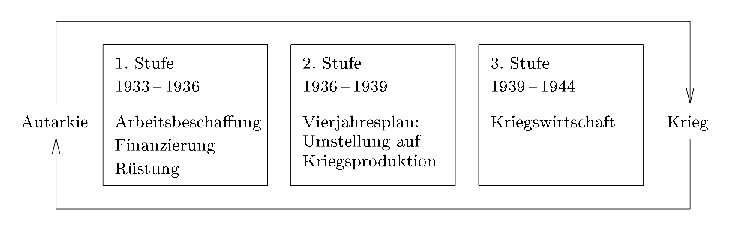
\includegraphics[width=\textwidth]{hit-stufpla.eps}
\caption{\Nam{Hitler, Adolf}{Hitler}s Stufenplan}
\label{pic:hit-stufpla}
\end{figure}

Diese Ziele wollte \Nam{Hitler, Adolf}{Hitler} mit seinem
\ges{Stufenplan} (siehe \ref{pic:hit-stufpla}) erreichen. Dessen erste
Stufe soll hier näher beleuchtet werden. \mar{Und die anderen?}

Die dargestellten Maßnahmen folgten der Politik des \emph{deficit
spending}\index{deficit spending}, welches durch den
Reichswirtschaftsminister und Reichsbankpräsidenten \Nam{Schacht,
Hjalmar}{Hjalmar Schacht} angeregt wurde. Er erfand auch das
sogenannte \emph{Mefo-Wechselsystem}\index{Mefo-Wechsel} zur
Finanzierung der Rüstungsaufträge. Nach diesem bezahlte nicht das
Deutsche Reich direkt selbst, sondern eine Scheinfirma, die \Ins{Mefo,
Metallurgische Forschungsgesellschaft}{Metallurgische
Forschungsgesellschaft} (Mefo) akzeptierte von der Industrie
ausgestellte Wechsel, die bis 1938 einzulösen waren. Die weiteren
Details sind hier unwichtig. Dieses System bot einige
Vorteile.\mar{Doch welche?}


\subsection{Erste Stufe: Wirtschafts- und
Sozialpolitik\mycite{LemoWirtsch}}
\mar{Wo sind die anderen?}

\subsubsection{wirtschaftliche Maßnahmen:}

\begin{itemize}
\item leichter Wirtschaftsaufschung 1933 durch die
Arbeitsbeschaffungsmaßnahmen der vorherigen Regierungen
\item Arbeitsbeschaffungsprogramme (Straßenbau: Autobahn, Bauwesen:
Wohnungsbau) steuerliche Anreize $\Rightarrow$ Senkung der
Arbeitslosigkeit
\item ab \dat{Juni 1935 Reichsarbeits- und Wehrdienst} $\Rightarrow$
Senkung der Arbeitslosigkeit
\item NS-Regime baut auf Privateigentum -- Interessenübereinstimmung
zwischen Großindustrie (Profitgier) und NS-Regime (forcierte
Kriegsvorbereitung)
\item schnelle Aufrüstung der modernen Industriezweige, beispielsweise
des Fahrzeugbaus
\item öffentliche Wirtschaftsforderung, vor allem durch
Rüstungsaufträge
\item Förderung der Landwirtschaft durch das
\dat{\ges{Reichserbhofgesetz} vom 29. September 1933}, das 
Hofteilung, Verkauf und Belastung mit Hypotheken verbot, dadurch aber
auch Neuinvestitionen stark behinderte.
\end{itemize}

\subsubsection{sozialpolitische Maßnahmen:}

\begin{itemize}
\item 1. Mai als staatlicher Feiertag bei voller Lohnfortzahlung
(1933 \ins{Feiertag der nationalen Arbeit}, ab 1934 \ins{Nationaler
Feiertag}) \index{1. Mai}
\item Gründung der Organisation \dat{\ins{Kraft durch Freude} im
November 1933} $\Rightarrow$ kulturelle und touristische
Freizeitbeschäftigungen für große Teile der Arbeiterschaft
\item Sofortmaßnahmen gegen Hunger, Armut und Verelendung, darunter
die Gründung des \dat{\Ins{Winterhilfswerk}{Winterhilfswerks}}
\end{itemize}

\endinput

\section{Außenpolitik}

Liest man \Nam{Hitler, Adolf}{Hitler}s Regierungserklärung vor dem
Reichstag vom 17. Mai 1933\mycite{HitlRegErklFrie} und seine Rede vor
der Reichswehrführung in Berlin vom 3. Februar des selben
Jahres\mycite{HitlRedRwfueh}, wird der zweischneidige Charakter seiner
Außenpolitik deutlich: Während er vor dem Reichstag von einer Heilung
der Wunden des Versailler Vertrages innerhalb der Grenzen der Verträge
und durch friedliche Auseinandersetzung mit \enquote{den Nationen}
spricht, fordert er vor der Reichswehr einen \enquote{Kampf gegen
Versailles} und \enquote{Sorge für die Bundesgenossen} unter
Verwendung kriegerischer Mittel.

Man erkennt also eine Verschleierungstaktik, die die eigentliche
Kriegsvorbereitung durch den scheinbaren Weg über Verträge verdecken
sollte. Zu den konkreten Maßnahmen siehe Tabelle
\ref{tab:massn-hitl-ausspol}. Für Karikaturen zu dem Thema siehe den
Hefter.

\begin{table}
\caption{Außenpolitische Maßnahmen Hitlers}
\label{tab:massn-hitl-ausspol}

\begin{tabularx}{\textwidth}{cXX}
\toprule
Jahr    & verschleiernd     & kriegsvorbereitend \\ 
\midrule
1933 & Konkordat mit dem Papst\index{Reichskonkordat} & \\
     & \multicolumn{2}{c}{Austritt aus dem
Völkerbund}\index{Völkerbund!Austritt des Deutschen Reiches}   \\

1934 & \ges{Deutsch-Polnischerr -Nichtangriffspakt} &  \\

1935 & Rückgliederung des Saarlands
(Volksabstimmung)\index{Saarland!Rückgliederung} &  \\
     & \ges{Flottenabkommen} mit Großbritannien &  \\

1936 & \Ins{Olympische Spiele!Deutschland}{Olympische Spiele} in
Deutschland & Rheinlandbesetzung \index{Rheinland!Besetzung} \\

1937 &  & Beitritt Italiens zum \ges{Antikominternpakt} -- \ins{Achse
Berlin\,--\,Rom\,--\,Tokio}\\

1938 &  & Anschluss Österreichs\index{Österreich!Anschluss an das
Deutsche Reich} \\

     &  & Sudetenkrise\index{Sudetenkrise} -- \ges{Münchener Abkommen} \\

1939 &  & \ges{Deutsch-Sowjetischer Nichtangriffspakt} mit geheimem
Zusatzprotokoll \index{Zusatzprotokoll} \\
\bottomrule
\end{tabularx}
\end{table}

\endinput

Hohohohohoho.

\section{Ausschaltung realer und vermeintlicher Gegner des NS-Regimes}
\label{sec:aussch-gegner}

\begin{aufgabe}
Erläutern Sie ideologische Grundlagen der Ausschaltung vermeintlicher
Gegner!

Beschreiben Sie die Umsetzung der Ideologie an den beiden
vermeintlichen Gegnergruppen! 

Bewerten sie die Maßnahmen auf der Basis demokratischer Politik- und
Moralvorstellungen!
\end{aufgabe}

\begin{aufgabe}
Arbeiten Sie aus dem Text die elemente des historischen Gesamtrahmen,
in dem sicher nationalsozialistische Massenmord entwickelten, heraus!

Der Autor behauptet, dass die Rolle Hitlers entscheindend für die
Judenverfolgung/-vernichtung war. Erarbeiten Sie die dazu gehörende
Argumentation anhand des Textes und die zu Grunde liegenden
ideologischen Ansätze!

\Nam{Friedländer, Saul}{Friedländer} nennt die ideologische
Radikalisierung des ausgehenden 19. Jahrhunderts als einen Faktor, der
in Kombination mit weiteren den Holocaust \enquote{vorbereitete}.
Überprüfen Sie diese Theorie der Radikalisierung innerhalb der
Maßnahmen des Regimes von 1933 bis 1945!
\end{aufgabe}


\begin{description}
\item[Grundlage:] Rassenideologie und Sozialdarwinismus
\index{Rassenideologie} \index{Sozialdarwinismus}
\item[Ziel:] Verhindern der Beeinträchtigung des \nat{deutschen
Volkskörpers} und Schaffung der \nat{reinen Rasse}
\end{description}

Die Höherentwicklung des deutschen Volkes (\nat{Herrenmensch}) wurde
laut Ideologie bedroht durch\footnote{Beide Bereiche greifen
ineinander. Die Trennung dient nur der Veranschaulichung.}\mar{Das ist
ein Fall von Scheinheiligkeit.}:

\begin{multicols}{2}
Unerwünschtes (\nat{lebensunwertes}) Leben:
\nat{schlechte Erbanlagen} bedrohen die Höherentwicklung des Volkes
sowie der Menschheit.

$\rightarrow$ \nat{Rassenhygiene}\\

\emph{Euthanasie}

\columnbreak

Juden und \nat{Art-}/\nat{Rassenfremde}: \nat{rassisch bedingte 
Verderbtheit der Juden als minderwertige Rasse}

$\rightarrow$ Rassenantisemitismus\\

\emph{\beg{Holocaust}}
\end{multicols}

%%%%%%%%%%%%%%%%%%%%%%%%%%%%%%%%%%%%%%%%%%%%%%%%%%%%%%%%%%%%%%%%%%%%%%

\subsection{Euthanasie}
\label{ssc:Euthanasie}
\index{Euthanasie}

\subsubsection{Gesetzliche Grundlagen}

\begin{chronik}
\item[14.\,7.\,1933] \ges{Gesetz zur Verhütung erbkranken Nachwuchses}:
Zwangssterilisierung von vermeintlich Erbranken -- circa 6\,000 Tote,
am meisten Frauen

\item[26.\,6.\,1935]
Ergänzung: Legalisierung des Schwangerschaftsabbruchs bei
diagnostizierter Erbkrankheit

\item[15.\,9.\,1935]
\ges{Gesetz zum Schutz des deutschen Blutes und der deutschen Ehre}:
siehe \ref{sss:nürnberger-ges}

\item[18.\,10.\,1935]
\ges{Ehegesundheitsgesetz}: Verbot von Eheschließungen mit geistig
Behinderten und Erbkranken

\item[1.\,9.\,1939]
\emph{Geheimer Führererlaß}: Ermächtigung zur Durchführung der
Euthanasie
\end{chronik}

\subsubsection{Aktion T4}
\index{Aktion T4}

\setlength{\parskip}{0mm}

Diese nach dem Krieg nach der Adresse -- Tiergartenstraße 4 -- der
Euthanasiezentrale in Berlin benannte Aktion beinhaltete die Umsetzung
des Euthanasiebefehls. Der daran beteiligte Personenkreis teilte
sich in vier Aufgabenbereiche:

Die \ins{Reichsarbeitsgemeinschaft Heil- und Pflegeanstalten} (Leiter:
\Nam{Heyde, Werner}{Werner Heyde} (medizinisch), \Nam{Bohne,
Gerhard}{Gerhard Bohne} (Verwaltung)) war für die Erfassung der Opfer
zuständig und verschickte zu diesem Zweck ab Ende 1939 Meldebögen, die
Auskunft über Art und Dauer der Krankheit und die Arbeitsfähigkeit
verlangten.

Die \ins{Gemeinnützige Stiftung für Anstaltspflege} (Leiter:
\Nam{Schneider, Willy}{Willy Schneider}) diente als offizieller
Arbeitgeber der etwa 400 T4-Mitarbeiter.

Die \ins{Zentralverrechnungsstelle Heil- und Pflegeanstalten} (Leiter:
\Nam{Kaufmann, Gustav a.}{Gustav A. Kaufmann}) wickelte die Kosten ab.

Die \ins{Gemeinnützige Krankentransport GmbH} (Leiter: \Nam{Vorberg,
Reinhold}{Reinhold Vorberg}) fuhr mit meist grauen Bussen die Opfer in
die Zwischen- beziehungsweise Tötungsanstalten.\\

\noindent Die Aktion T4 begann 1939 mit der Kindereuthanasie, dem
an mindestens 5\,000 erbkranken oder behinderte Kindern und
Säuglingen.  Wenig später wurden die Tötungen auf Erwachsene
ausgeweitet. Etwa 70\,000 geistig Behinderte, psychisch Kranke, mehr
als fünf Monate stationär Behandelte, Straftäter und
\nat{Fremdrassige} wurden dabei vergast.

Aufgrund von Protesten der Kirche, der Angehörigen und in der
Bevölkerung stellte man die Vergasungsaktionen 1941 offiziell ein. Da
man aber wegen des Luftkriegs gegen Deutschland immer mehr
Krankenhausplätze benötigte, begann nun die sogenannte \emph{Wilde
Euthanasie}\index{Wilde Euthanasie}: Etwa 30\,000 Menschen wurden
heimlich vergiftet oder zu Tode gehungert.

%%%%%%%%%%%%%%%%%%%%%%%%%%%%%%%%%%%%%%%%%%%%%%%%%%%%%%%%%%%%%%%%%%%%%%

\subsection{Die Verfolgung der Juden}
\label{ssc:juden-verf}
\index{Holocaust}
\index{Judenverfolgung}

% Breite der ersten Spalte
\newlength{\frstcoljud}
\settowidth{\frstcoljud}{Phase}
% Breite der übrigen Spalten
\newlength{\othcol}
\newlength{\othcolsum} % der ganze Rest
\setlength{\othcolsum}{\textwidth}
\addtolength{\othcolsum}{-\frstcoljud}
\setlength{\othcol}{0.25\othcolsum}
\addtolength{\othcol}{-2\tabcolsep}

\begin{tabular*}{\textwidth}{p{\frstcoljud}*{4}{p{\othcol}}}
Phase & \Rm{1} & \Rm{2} & \Rm{3} & \Rm{4} \\
      & 1933-35 & 1935-38 & 1938-41 & 1941-45 \\
      & Boykottaktio"-nen & Ausgrenzung durch Gesetz und Terror
      & Deportation & Endlösung
\end{tabular*}

\subsubsection{Boykottaktionen\mycite[135, 136]{GeschDrReich}}
\label{sss:boykott}
\index{Judenboykott}

\begin{chronik}
\item[1.\,--\,3.\,4.\,1933]
befristeter\footnote{Laut Frau Seipold schlug die Aktion fehl, da die
Bevölkerung aus Gewohnheit weiter bei Juden einkaufte.
\cite[135]{GeschDrReich} stellt das etwas anders beziehungsweise
differenzierter dar.} Boykott jüdischer Geschäfte\footnote{Diese
Aktion bildete das Ende der spontanen Gewalt gegen die jüdische
Bevölkerung. Was folgte, waren organisierte Verbrechen.}

\item[7.\,4.\,1933]
\ges{Gesetz zur Wiederherstellung des Berufsbeamtentums} (ein Art
staatlicher \emph{Arierparagraph}): Entlassung von
\nat{\beg{Nicht-Ariern}} aus dem öffentlichen Dienst

\item[7.\,4.\,1933]
Möglichkeit des Entzugs der Zulassung jüdischer Anwälte

\item[April 1933]
\ges{Gesetz gegen die Überfüllung der deutschen Schulen und
Hochschulen}: Verdrängung der Juden aus den
Bildungsanstalten\footnote{Der vollständige Ausschluß erfolgte 1938.}

\item[5.\,10.\,1933]
\ges{Schriftleitergesetz}: Verdrängung jüdischer Journalisten aus den
Redaktionen

\item[1934]
Pause von antijüdischen Gesetzen
\end{chronik}


\subsubsection[\dat{Nürnberger Gesetze 15. September 1935}]
{\dat{Nürnberger Gesetze 15. September 1935}
\mycite[417-419]{gelbesGeschichts}}
\label{sss:nürnberger-ges}
\index{Nürnberger Gesetze}

\paragraph{\ges{Reichsbürgergesetz}} 
Juden verloren alle politischen Bürgerrechte -- sie wurden statt
als \nat{Reichsbürger} nur noch als \nat{Staatsangehörige}
gesehen und somit aus der \emph{Volksgemeinschaft} ausgeschlossen.

\paragraph{\ges{Gesetz zum Schutz des deutschen Blutes und der
deutschen Ehre}}
Diese Gesetz verbot Juden

\begin{itemize}
\item Ehen und außereheliche Beziehungen mit \nat{Ariern}
\item die Beschäftigung \nat{arischer} Dienstmädchen unter 45
Jahren
\item das Hissen der \nat{Reichs- und Nationalflagge} und das
Zeigen der \nat{Reichsfarben}
\end{itemize}

In den Folgejahren wurden die Rechte der Juden durch Sondergesetze und
Verordnungen immer weiter eingeschränkt,
beispielsweise\footnote{In \cite[135-137]{GeschDrReich} ist dies
differenziert dargestellt.}:

\begin{itemize}
\item Entfernung aus Beamtenpositionen und Wegfall der Pensionen
\item Boykottierung jüdischer Geschäftsleute und Industrieller
\item Entzug jeglichen Rechtsschutzes
\item Ungültigmachung mit Juden geschlossener Verträge
\item Zutrittsverbot zu Hotels, Pensionen, kulturellen Einrichtungen
und Parks
\end{itemize}

\noindent $\Longrightarrow$ völlige Entrechtung und gesellschaftliche
Isolierung der Juden \\

Im Hinblick auf die \dat{Olympischen Spiele} in Deutschland reduzierte
man die Repressalien \dat{1936} wieder, nur um sie im folgenden Jahr
erneut zu forcieren.


\subsubsection{\dat{Reichspogromnacht 9./10. November 1938}}
\label{sss:pogromnacht}
\index{Reichspogromnacht}
\index{Reichskristallnacht}

Am \dat{7. November 1938} verübte \Nam{Grynspan, Herschel}{Herschel
Grynszpan} in Paris ein Attentat auf den dortigen Botschaftssekretär
\Nam{Rath, Ernst vom}{Ernst vom Rath}.  Dieses nahmen die
Nationalsozialisten in Deutschland zum Anlaß und Vorwand für
gewaltsame Aussshreitungen gegen Deutsche jüdischen Glaubens zwei Tage
später.

Im Zuge derer kam es zu Morden und Plünderungen, Synagogen, jüdische
Gebetshäuser, Friedhöfe, Geschäfte und Wohnungen wurden in Brand
gesteckt beziehungsweise zerstört. Der Name \emph{Reichskristallnacht}
rührt von den zahlreichen Fensterscheiben her, die in jener Nacht
zerschlagen wurden.

Die Folgen der \emph{Novemberpogrome} waren mindestens 1\,300 Tote,
mehr als 1\,400 zerstörte Synagogen, Verhaftungen und Deportationen
und weitere Verschlechterung der Lebensbedingungen für Juden. Für die
entstandenen Schäden von ungefähr 1,12 Milliarden Reichsmark mußten
die Opfer selbst aufkommen.

Mit dem endgültigen Verlust finanzieller Mittel wurde den Juden eine
eventuelle Ausreise aus noch weiter erschwert.


\subsubsection[Radikalisierung der Judenpolitik \dat{September
1939\,--\,1941}]
{Radikalisierung der Judenpolitik \dat{September
1939\,--\,1941}\mycite[209, 216]{GeschDrReich}\mycite[433,
434]{gelbesGeschichts}}
\label{sss:rad-jud-pol}

\paragraph{Deportationsmaßnahmen/-pläne} \index{Deportation}
Durch ihre Kriegserfolge angespornt, stellten die Nationalsozialisten
verschiedene Pläne, die Juden aus Europa zu verbannen, auf. Diese
wurde jedoch aufgrund der schieren Anzahl zu Deportierender nicht
umgesetzt: 

\begin{chronik}
\item[1939\,--\,1941]
Zwangsumsiedlung nach Polen, Zusammenfassung und Isolierung in
\beg{Ghettos} \index{Ghetto}

\item[1940]
(Sieg über Frankreich): \beg{Madagaskarplan} \index{Madagaskarplan}

\item[1941]
(Überfall auf die UdSSR): Umsiedlung nach Sibirien
\end{chronik}


\paragraph{Vorgehen der SS-Einsatztrup"-pen beim Überfall auf Polen}
während des Überfalls auf Polen führten die SS-Einsatztrup"-pen im
Schatten der Wehrmacht \nat{politische Säuberungen} durch: Mit dem
iel der Ausrottung der jüdischen Bevölkerung kam es zu
assenerschießungen und Massakern. In den ersten Kriegswochen starben
abei circa 5\,000 Menschen.

ußerdem wurde die Kennzeichnungspflicht für Juden eingeführt und
man pferchte sie in Ghettos zusammen, wo sie Zwangsarbeit für die
Rüstungsindustrie zu leisten hatten.

\paragraph{Vertreibung der Juden nach dem Polenfeldzug}
\index{Deportation}
Mit der Begründung, Wohnraum werde \nat{aus kriegswirtschaftlichen
Gründen dringend benötigt}, deportierte man die Juden in Lager
in der Gegend von Lublin und im \ort{Generalgouvernement}. Das geschah
zunächst Bewohnern des \ort{Gaus Warteland}, ein halbes Jahr später
denen aus \ort{Pommern}. Im \dat{Februar 1940} vertrieb man die
Juden aus der Gegend von \ort{Stettin} und im \dat{März 1940} aus
\ort{Schneidemühl} in Preußen.

\paragraph{Vorgehen gegen die jüdische Bevölkerung während des
Krieges gegen die Sowjetunion}
Mit dem Krieg gegen die UdSSR wurden die Tötungsaktionen des Überfalls
auf Polen fortgesetzt. Neben der Wehrmacht, die dabei in die
Machenschaften der SS integriert wurde, rekrutierte man nun auch Teile
der Bevölkerung als \nat{Reserve-Polizeibataillone} sowie verbündete
Truppen, vor allem aus Weißrußland und Rumänien.

Von den 4,7 Millionen sowjetischen Juden kamen so bis Ende 1942 2,2
Millionen zu Tode.


\subsubsection{Konzentrations- und Vernichtungslager -- Die
\nat{Endlösung der Judenfrage}}
\label{sss:konz-vern-endl}
\index{Konzentrationslager}
\index{Vernichtungslager}
\index{Endlösung}

\begin{chronik}
\item[Juni 1941]
Vergasungsanlagen für \ort{Auschwitz}, Einsatz ab Herbst als
Vernichtungslager\footnote{Nach \ort{Chełmno}, wo noch die sogenannten
\ort{Gaswagen} verwendet wurden\cite{WikChelmno}, war es damit das
zweite Vernichtungslager und sollte das größte derer werden.}

\item[31.\,7.\,1941] Anweisung an \Nam{Heydrich, Erwin}{Reinhard
Heydrich}, eine \nat{Endlösung der Judenfrage} zu finden

\item[20.\,1.\,1942]
\emph{Wannseekonferenz}:
\begin{itemize}
\item Organisation und Koordination der Deportation der europäischen
Juden
\item Beschluß, Juden in ganz Europa als Arbeistkräfte auszubeuten und
zu ermorden\footnote{Laut \cite{WikWannsee} war dieser Beschluß
faktisch schon gefaßt. Ich füge ihn hier ein, da sich kein anderer
Platz ergeben hat.}
\end{itemize}

\item[1942]
Errichtung weiterer Vernichtungslager in \ort{Bełżec}, \ort{Sobibór},
\ort{Treblinka} und \ort{Majdanek}
\end{chronik}

\endinput

\section[Widerstand]{Widerstand\mycite[116-125, 230-245]{GeschDrReich}}
\label{sec:widerstand}
\index{Widerstand gegen den Nationalsozialismus}

\begin{aufgabe}
Begründen Sie, warum trotz der Radikalität und Unmenschlichkeit des
Regimes der innerdeutsche Widerstand realtiv begrenzt blieb! 
\end{aufgabe}

\subsection[Definition]{Definition\mycite{WidDefschwieBeg}}

Es gibt immer wieder Debatten, wie der Begriff des Widerstands im
Nationalsozialismus zu definieren sei.\footnote{Selbst das hier
verwendete \cite{WidDefschwieBeg} weist hier Fehler in der logischen
Durchführung auf.} So schlug \Nam{Broszat, Martin}{Martin Broszat} in
den frühen Achtzigerjahren vor: \enquote{Wirksame Abwehr, Begrenzung,
Eindämmung der NS-Herrschaft oder ihres Anspruchs, gleichgültig von
welchen Motiven, Gründen und Kräften her.}

Es gab jedoch zahlreiche Kritik, die entgegesetzte, dass jene
Definition den Begriff zu weit fasse und schon bei \emph{Haltungen}
beginne, während man erst bei \emph{Handlungen} einsetzen
dürfe.\footnote{Ich bin anderer Ansicht. \enquote{Wirksame Abwehr,
Begrenzung, Eindämmung} sind für mich keine bloßen Haltungen.}
Weiterhin greift man die fehlende Berücksichtigung der Motive an.

Die Tendenz geht als hin zum Widerstand als
\textquote[\mycite{WidDefschwieBeg}]{Handeln, das auf grundsätzlicher
Ablehnung des Nationalsozialismus beruhte, das aus ethischen,
politischen, religiösen, soialen oder individuellen Motiven darauf
abzielte, zum Ende des Regimes beizutragen}.

Tabelle \ref{tab:widerst-def} gibt einen Überblick über verschiedene
Möglichkeiten der Definition.

% verfluchter Blocksatz
\begin{table}
\caption{Definitionen für \emph{Widerstand}\mycite{WidDefschwieBeg}}
\label{tab:widerst-def}

% Berechnung der Spaltenbreiten
\newlength{\colwidth}
\setlength{\colwidth}{0.33\textwidth}
\addtolength{\colwidth}{-2\tabcolsep}

\renewcommand*{\arraystretch}{1.5}

\begin{tabular*}{\textwidth}{*{3}{p{\colwidth}}}
\toprule

\multirow{2}{\colwidth}{\centering Widerstand im weitesten Sinn} &
\multicolumn{2}{c}{Widerstand im engeren Sinn} \\

\cmidrule{2-3}

&
kritische bis abweisende Haltung der Verweigerung und Selbstbehauptung
&
bewusste Anstrengung zur Änderung der Verhältnisse \\

\midrule

zusammenfassender Oberbegriff für gegen den Nationalsozialismus als
Ideologie und praktizierte Herrschaft gerichtete verschiedenartige
Einstellungen, Haltungen und Handlungen &
\emph{Verweigerung} als persönliche Abwehr von Herrschaftsanspruch und
Selbstbehauptung von Gruppen &
bewusster persönlicher Einsatz, verbunden mit einhergehenden
Gefährdungen \\

Umfasst also auch beispielsweise ins Exil geflohene, die kaum
Möglichkeit zur Einwirkung auf das nationalsozialistische Regime
hatten und die die sich weder durch Lockungen noch durch Zwang vom
Nationalsozialismus vereinnahmen ließen. &
\emph{Opposition} als Haltung grundsätzlicher Gegnerschaft gegen das
Unrechtsregime -- passiver Widerstand &
beispielsweise Planung des Sturzes der Diktatur (Attentate)
einhergehend mit der Errichtung einer neuen Gesellschaftsordnung --
aktiver Widerstand \\

\bottomrule 
\end{tabular*}
\end{table}

%%%%%%%%%%%%%%%%%%%%%%%%%%%%%%%%%%%%%%%%%%%%%%%%%%%%%%%%%%%%%%%%%%%%%%

\subsection{Gruppen}

Die deutschen Widerstandsgruppen kamen aus verschiedenen
gesellschaftlichen Schichten. Dabei ist der Mittelstand kaum
ernennenswert; dessen größte Teile waren dem \index{Hitler-Mythos}
Hitler-Mythos erlegen.

Etwas mehr, aber dennoch nur wenig, tat sich bei den Vertretern der
Industrie: Hier waren es hauptsächlich \Nam{Bosch, Robert}{Bosch} und
\Nam{Krupp von Bohlen und Halbach, Gustav}{Krupp}, die \Nam{Goerdeler,
Carl Friedrich}{Goerdeler} unterstützten und andere, die Kontakte zum
amerikanischen Geheimdienst unterhielten. Inwiefern man dabei jeweils
von \emph{Widerstand} sprechen kann, ist natürlich fragliche.

Schließlich formierten sich im politischen Lager zahlreiche locker
zusammengeschlossene Gruppen, die aber meist nur das gemeinsame Ziel
der Beseitigung des Regimes verband.

Alle waren allerdings der Meinung, dass die Befreiung vom
Nationalsozialismus von Deutschland selbst aus erfolgen müsse, da nur
so eine \emph{bedingungslose Kapitulation}, wie sie die Alliierten
forderten abgewendet und Souveränität und Verhandlungsfähigkeit
Deutschlands erhalten werden könnten.\mycite[191-193]{DeuzwDemuDikt}

Dabei waren die Widerstandsbewegungen im Ausland, beispielsweise die
\ins{R\'e{}sistance} in Frankreich und \index{Partisanen}
\ins{Partisanengruppen} in Polen, der Sowjetunion, Jugoslawien,
Griechenland und Italien, zum Teil viel reger und erfolgreicher als im
Reich selbst. Das lag daran, dass sich die politischen und geistigen
Strömung unter dem Eindruck eines gemeinsamen Besatzers zu einem
nationalen Befreiungskampf einten, während die Widerstandsgruppen in
Deutschland nur wenig zusammenarbeiteten, während die
Widerstandsgruppen in Deutschland nur wenig zusammenarbeiteten.

Anfangserfolge im Krieg hatten den \index{Hitler-Mythos} Hitler-Mythos
befeuert, Beamte und andere hatten einen Eid auf \Nam{Hitler,
Adolf}{Hitler} geschworen. Der Terror durch die \ins{Gestapo} und
scharfe Gesetze, die Kritik am Regime und Kontakte zum Ausland und zu
Ausländern im Inland verboten, taten ihr Übriges, um eine
Ablehnungshaltung der Bevölkerung gegenüber Widerständlern und
gewaltsamer Beseitigung der Obrigkeit zu schaffen.

Allerdings kehrte sich diese Haltung mit fortschreitendem
Kriegsverlauf immer weiter ins Gegenteil. Die Verschlechterung des
Zustands, insbesondere der Versorgungslage, ließ den Wunsch nach
baldigem Kriegsende immer größer werden; die unerwartete Kriegslage
verunsicherte das Regime, die Herrschaftsstruktur wurde löchrige,
sodass die Bevölkerung allmählich das Vertrauen verlor.

Im Folgenden sollen beispielhaft einige Gruppen mit ihren Motiven,
Zielen und Handlungen aufgeführt werden, die sich auch schon vor den
meisten Anderen gegen die nationalsozialistische Herrschaft gerichtet
hatte. Dabei werden sämtliche Grade von Kritik bis zum aktiven
Widerstand berücksichtigt.


\subsubsection[Kommunisten und Sozialdemokraten]{Kommunisten und
Sozialdemokraten\footnote{Die beiden Gruppen wirkten keineswegs von
Anfang an gemeinsam im Widerstand und auch später gab es teilweise
große Differenzen. So kämpften die Kommunisten zunächst ebenso gegen
die Sozialdemokraten und auch die Wahl der Mittel fiel unterschiedlich
aus: Während die Ersteren einigermaßen radikal und ohne Rücksicht auf
Verluste vorgingen, während die Anderen mehr Vorsicht walten ließen.}}
\index{Kommunismus}
\index{Sozialdemokratie}

Für deren Aktivitäten lagen natürlich ideologische Gründe vor.

\noindent Mittel:

\begin{itemize}
\item Flugblätter und Broschüren in großer Anzahl
\item Wandparolen
\item Demonstrationen
\item Fahnenhissen
\item Sprechchöre
\item Überzeugungsarbeit \enquote{von Mann zu Mann}
\item stille Verweigerung und
\textquote[{\mycite[120]{GeschDrReich}}]{öffentliche[s] Beharren auf
demokratischen und rechtsstaatlichen Idealen}
\item Milieubildung mit Nachbarschaftshilfe, Austausch von Meinungen,
Nachrichten und Spende von Trost
\item Fluchthilfe
\item Abhören ausländischer Sender
\item Zeitschriften und Publikationen, auch für das Ausland
\end{itemize}


\subsubsection{Kirchen}
\index{Widerstand!Kirchen}

Auch die Kirchen waren untereinander in ihrer Haltung gegenüber dem
Nationalsozialismus gespalten. Während die Katholiken sich zunächst
von \Nam{Hitler, Adolf}{Hitler} betören und täuschen ließen und später
eher seichte Mahnungen an das Regime richteten, wurde das anfängliche
Verlangen der Protestanten nach einem \nat{starken Mann} an der Spitze
des Staates befriedigt.

Allerdings vollzog sich mit der Zeit eine zunehmende Spaltung der
evangelischen Kirche in \Ins{Deutsche Christen}{Deutschen Christen}
als Anhänger des Nationalsozialismus und die \ins{Bekennende Kirche},
die ein entschlosseneres Unternehmen als die Katholiken an den Tag
legte.

Trotzdem muss man erkennen, dass weniger die Kirchen als Institutionen
selbst Widerstand leisteten, sondern eher christliche Einzelpersonen
-- besonders prominent sicherlich \Nam{Niemöller, Martin}{Martin
Niemöller} und \Nam{Bonhoeffer, Dietrich}{Dietrich Bonhoeffer} --
offen gegen den Nationalsozialismus vorgingen.\\

\noindent Kritikpunkte:

\begin{sloppypar}
\begin{itemize}
\item Kampf gegen Ordensgemeinschaften
(\nat{Klostersturm}\index{Klostersturm})
\item \textquote[{\mycite[121]{GeschDrReich}}]{\enquote{Pfaffenprozesse}
\index{Pfaffenprozesse} gegen Ordensgeistliche wegen angeblicher
Devisenschiebereien und Sittlichkeitsvergehen}
\item Eingriff des Staats in Kirchenangelegenheiten
\item Missachtung des \Ges{Reichskonkordat}{Reichskonkordats}
\item Rassenpolitik, Antisemitismus
\item Euthanasie
\item \nat{rassisch-völkische Weltanschauung}
\item Konzentrationslager
\item Willkür der \ins{Gestapo}
\item Missachtung christlicher Grundsätze
\end{itemize}
\end{sloppypar}

\noindent Mittel:

\begin{itemize}
\item Enzyklika \index{Enzyklika} \ges{Mit brennender Sorge}, geheim
vervielfältigt und verteilt
\item Eingaben\footnote{Diese waren eher zurückhaltender Art und
natürlich auch kaum erfolgreich.}
\item Reden von der Kanzel aus -- Predigten
\item \ins{Pfarrernotbund}
\item Untergrundarbeit
\end{itemize}


\subsubsection{Kreis um \Nam{Goerdeler, Carl Friedrich}{Carl Goerdeler}}

Hierzu gehörten hochrangige Militärs (beispielsweise \Nam{Beck,
Ludwig}{Generaloberst Ludwig Beck}), Wirtschaftsverantwortliche,
Industrielle, Gewerkschafter und andere vornehmlich konservative,
christliche und nationalliberale Bürger und Politiker. \\

\noindent Kritikpunkte:

\begin{itemize}
\item waghalsige Kredit-, Finanz- und Wirtschaftspolitik
\item Antisemitismus (negative Wirkung auf das Ansehen Deutschlands im
Ausland)
\item Entfernung des Denkmals für \Nam{Mendelssohn-Bartholdy,
Felix}{Felix Mendelssohn-Bartholdy} in Leipzig
\item Unterschätzung des Auslands
\item Kriegsbestrebungen
\end{itemize}

\noindent Ziele:

\begin{itemize}
\item Staatsstreich
\item Staats- und Gesellschaftsordnung auf Grundlage von
Rechtsstaatlichkeit, Moral, bürgerlichem Anstand und christlicher
Weltanschauung -- stark restaurativer Charakter
\item Kriegsende
\end{itemize}

\noindent Mittel:

\begin{itemize}
\item Kritik in Wirtschaftsgutachten für die Regierung
\item Werbung für Opposition gegen die Nationalsozialisten im Ausland
\item Knüpfung von Beziehungen zu Personen in verschiedensten
gesellschaftlichen Positionen
\item Einsatz des Militärs -- Verhandlungen mit hochrangigen
Offizieren
\end{itemize}


\subsubsection{Kreisauer Kreis\index{Kreisauer Kreis}}

Hier handelte es ich um eine Gruppe von Regimegegner
unterschiedlichster Profession, die sich auf dem Gut des \Nam{Moltke,
Helmuth James Graf von}{Helmuth James Graf von Moltke} in
\ort{Kreisau}, \ort{Niederschlesien}, zu Gesprächen traf. Führender
Kopf war neben dem Gutsbesitzer \Nam{Wartenburg, Peter Graf Yorck
von}{Peter Graf Yorck von Wartenburg}.

Bei dieser Gruppe muss man außerdem hervorheben, dass sie
hauptsächlich von den Verbrechen der Nationalsozialisten gegen Juden,
Kriegsgefangene und Bewohner der besetzten Gebiete zum Widerstand
angeregt wurden. Das war bei den bisher genannten Personen und
Körperschaften nicht primär der Fall.\\

\noindent Ziele\footnote{In diesem Abschnitt werden zahlreiche
Wortkombinationen verwendet, wie sie genau so in
\cite[236-238]{GeschDrReich} zu finden sind. Ich verzichte auf
ständige Anführungszeichen und Partikulärnachweise.}:

\begin{itemize}
\item Überwindung des Nationalsozialismus, des Machtstaats und des
Rassendenkens

\item Neuordnung und Neuorientierung von Staat und Gesellschaft
\begin{itemize}
\item Wiederherstellung eines humanen Rechtsstaats
\item Garantie von Glaubens- und Gewissensfreiheit
\item Recht auf Arbeit und Eigentum
\item Selbstbestimmung und Verantwortlichkeit statt Befehl und
Gehorsam
\item politische Verantwortung und Mitwirkung jedes Einzelnen statt
Diktatur und Unterwerfung
\item Gründung einer Völkergemeinschaft im Geiste internationaler
Toleranz
\end{itemize}

\item Bestrafung der nationalsozialistischen Verbrecher
\end{itemize}

\noindent Prinzipien:

\begin{itemize}
\item Humanität
\item christliche Ethik
\item Gerechtigkeit
\item Ablehnung von Gewalt\footnote{Hiermit ist hauptsächlich die
Ablehung eines gewaltsamen Sturzes des Regimes und einer Ermordung
\Nam{Hitler, Adolf}{Hitlers} gemeint. \Nam{Moltke, Helmuth James Graf
von}{Moltke} befürchtete nämlich, dass ein solches Vorgehen nach dem
Umsturz ähnlich der \emph{Dolchstoßlegende}\index{Dolchstoßlegende}
propagandistisch ausgeschlachtet würde.}
\end{itemize}


\subsubsection{Weitere}

Mit den genannten Gruppen ist ein großer Teil des Spektrums der Motive
und Ziele von Widerstandsgruppen abgedeckt. Für weitere Informationen,
insbesondere über die Attentate auf \Nam{Hitler, Adolf}{Hitler} und
über studentischen Widerstand wie den der \Ins{Weiße Rose}{Weißen
Rose} siehe auch \cite[239-245]{GeschDrReich}.

\endinput


\endinput

\part{Demokratie und Diktatur -- Anspruch und Wirklichkeit von
Gesellschaftsmodellen in der zweiten Hälfte des 20. Jahrhunderts}
\label{prt:dem-dikt2}
\thispagestyle{empty}

\chapter{Neubeginn im besiegten Land}
\label{sec:neubeginn}

\begin{chronik}
\item[8.\,5.\,1945]
bedingugslose Kapitulation Deutschlands -- offizielles Ende des
\emph{Zweiten Weltkriegs} \index{Zweiter Weltkrieg!Ende}

\item[5.\,6.\,1945]
\ges{Berliner Erklärung} \index{Berliner Erklärung} (USA,
Großbritannien, Frankreich, UdSSR): Übernahme der Regierungsgewalt und
des Oberkommandos der Wehrmacht durch die Alliierten

\item[17.\,7.\,--\,2.\,8.\,1945]
\ort{Postdamer} Konferenz \index{Potsdamer Konferenz}
\begin{itemize}
\item Aufteilung Deutschlands in vier Besatzungszonen
\index{Besatzungszonen}
\item Betrachtung der deutschen Wirtschaft als Einheit
\item Ziele: Dezentralisierung, Demokratisierung, Entmilitarisierung,
Entnazifizierung \index{Demokratisierung} \index{Dezentralisierung}
\index{Entnazifizierung} \index{Entmilitarisierung}
\item beinahes Scheitern der Verhandlungen über den Fragen der
Reparationen und der Ostgrenze
\end{itemize}
\end{chronik}

\section[Gründung der BRD]{Die Gründung der BRD\footnote{Es
handelt sich hier nur um einen groben Überblick. \label{ftn:grob-ueb}}
\mycite[333, 334]{WeltgeschNeuz}}
\label{sec:gruend-brd}
\index{BRD!Gründung}

\begin{chronik}
\item[Juli 1948]
Überreichung der \ges{Frankfurter Dokumente} an die
Ministerpräsidenten der Länder: Angebot zur Errichtung eines
westdeutschen Bundesstaates, Grundsätze für dessen Verfassung

\item[August 1948]
Erarbeitung eines Verfassungsentwurfes durch eine
Sachverständigenkommission als Beratungsgrundlage für den
\textsc{\Ins{Parlamentarischer Rat}{Parlamentarischen Rat}}

\item[8.\,5.\,1949]
Verabschiedung des Grundgesetzes durch den parlamentarischen Rat

\item[12.\,--\,23.\,5.\,1949]
Zustimmung der Westalliierten und der Bundesländer\footnote{Bayern
ratifizierte das Grundgesetz nicht, erkannte aber dessen
Rechtsverbindlichkeit an.} zum Grundgesetz 

\item[23.\,5.\,1949]
Inkrafttreten des \Ges{Grundgesetz für die Bundesrepublik
Deutschland}{Grundgesetzes für die Bundesrepublik Deutschland}

\item[14.\,8.\,1949]
freie, geheime, gleiche, direkte und allgemeine Wahl des ersten
\Ins{Deutscher Bundestag}{Deutschen Bundestages} durch die
westdeutsche Bevölkerung
\end{chronik}

\section[Gründung der DDR]{Die Gründung der DDR
\footref{ftn:grob-ueb}
\mycite[334, 335]{WeltgeschNeuz}}
\label{sec:gruend-ddr}
\index{DDR!Gründung}

\begin{chronik}
\item[10.\,7.\,1945]
zentrale Zulassung von Parteien in der \textsf{\ort{SBZ}} durch die
\beg{SMAD}

\item[14.\,7.\,1945]
Gründung des \Ins{Block antifaschistisch-demokratischer
Parteien}{Blocks antifaschistisch-demokratischer Parteien} --
Zusammenarbeit von KPD, SPD, CDU und LDPD
\begin{itemize}
\item nur einstimmige Beschlussfassung
\item Bindung für alle Parteien an die Beschlüsse
\item Festlegung eines nicht näher definierten gemeinsamen Weges
\end{itemize}

\item[22.\,4.\,1946]
Auf Druck der sowjetischen Gesatzungsmacht vereinigen sich SPD und KPD
zur SED\index{SED!Gründung}, da man befürchtete, dass die KPD in
freien Wahlen nicht genügend Stimmen gewinne.

\item[Feb. 1946]
Gründung des \textsf{\ins{FDGB}}\index{FDGB!Gründung}
(Einheitsorganisation) -- Während zwar
alle Parteien in der Leitung vertreten waren, sicherten sich die
Kommunisten dennoch die Vorherrschaft.

\item[Mitte März 1948]
Zusammentreten des \Ins{Zweiter Deutscher Volkskongresses}{Zweiten
Deutschen Volkskongresses} bestehend aus 2\,000
Delegierten\footnote{Die Stimmenmehrheit lag bei der SED und deren
Verbündeten} der Blockparteien und der Massenorganisationen
(beispielsweise FDJ und FDGB) auf Initiative der SED, Wahl des
\Ins{Deutscher Volksrat}{Deutschen Volksrates} (400 Mitglieder) --
Aufgabe: Ausarbeitung einer Verfassung für eine \enquote{unteilbare
deutsche Republik}

\item[19.\,3.\,1949]
Verabschiedung eines Verfassungsentwurfes durch den Deutschen Volksrat

\item[15./16.\,5.\,1949]
Wahl des \Ins{Dritter Deutscher Volkskongress}{Dritten Deutschen
Volkskongresses} durch die Bevölkerung der \ort{SBZ} nach
Einheitsliste.

Der \Ins{Dritter Deutscher Volkskongress}{Dritte Deutsche
Volkskongress} wählt den \Ins{Zweiter Deutscher Volksrat}{Zweiten
Deutschen Volksrat}, welcher sich zur provisorischen \ins{Volkskammer}
erklärt und die \ges{Verfassung der Deutschen Demokratischen Republik}
nach Bestätigung durch den \emph{Volkskongress} in Kraft setzt. Der
Präsident der DDR wurde \nam{Wilhelm Pieck}.

\item[7.\,10.\,1949]
Inkraftsetzung der \ges{Verfassung der Deutschen Demokratischen
Republik}

\item[15.\,10.\,1950]
Wahlen zur \ins{Volkskammer} über Einheitsliste\footnote{Artikel 51
der \ges{Verfassung der Deutschen Demokratischen Republik} sah
eigentlich eine Verhältniswahl vor.} durch die ostdeutsche
Bevölkerung
\end{chronik}

\endinput



\chapter{Das Demokratieverständnis in beiden deutschen Staaten}
\label{chp:demverst-beid-staat}
\index{Demokratieverständnis}

\section{Der Demokratiebegriff}
\label{sec:dem-begr}
\index{Demokratie}

\begin{aufgabe}
Untersuchen Sie, inwieweit die Verfassungen der neugegründeten Staaten
dem modernen Demokratiebegriff genügen!
\end{aufgabe}

\subsection*{Einteilung}

\begin{multicols}{2}
\noindent \emph{direkte Demokratie}:
direkte Entscheidungsfindung durch das Volk, beispielsweise in
Volksabstimmungen

\columnbreak

\noindent \emph{repräsentative (indirekte) Demokratie}:
Bürger wählen Repräsentanten, Sachentscheidungen durch Volksvertreter
\end{multicols}

\subsection*{Merkmale}

\begin{itemize}
\item Volkssouveränität (direkt, indirekt oder Mischform),
beispielsweise durch Wahlen oder Bürgerentscheide
\item Gewaltenteilung
\item Kontrolle der Exekutive und Legislative durch neutrale und
politisch unabhängige Judikative
\item Garantie der Menschen- und Bürgerrechte sowie der individuellen
Grundrechte (Schutz von Leben, Freiheit von Eigentum, Recht auf freie
Meinungsäußerung, Versammlungsfreiheit, Pressefreiheit)
\item Meinungspluralismus -- Parteienvielfalt
\item Verfassung
\end{itemize}

\endinput

\section[Volksaufstand in der DDR]{Volksaufstand in der
DDR\mycite{Dtl50erJ}}
\index{Voksaufstand}
\index{17. Juni 1953}

\subsection*{Ursachen}

\begin{itemize}
\item Militärblock- und Rüstungspolitik

\item Gründung der \Ins{Stasi, Ministerium für
Staatssicherheit}{Stasi} 1950 

\item wirtschaftliche Probleme:
\begin{itemize}
\item Planwirtschaft führt zu Priorisierung der Schwerindustrie und zu
Mangel in der Lebensmittel- und Konsumgüterproduktion
\item Rohstoffknappheit zwingt zu Importen
\item Reparationen
\item Ablehnung der Verstaatlichungsmaßnahmen (kaum noch
Privatwirtschaft), besonders in der Landwirtschaft führt zur
Auswanderung von Bauern und so zur weiteren
Verschärfung der Probleme.
\item Erhöhung der Arbeitsnorm
\end{itemize}

\item Unklarheit über die zukünftige Politik nach \Nam{Stalin,
Josef}{Stalin}s Tod am 5. Juni 1953

\item Erzwingung eines \jar{Neuen Kurses} durch die Sowjetunion am 9.
Juni:
\begin{itemize}
\item politische Lockerungen
\item Zugeständnisse an die Bauern und den Mittelstand
\item keine Rücknahme der Normerhöhung
\end{itemize}
\end{itemize}

%%%%%%%%%%%%%%%%%%%%%%%%%%%%%%%%%%%%%%%%%%%%%%%%%%%%%%%%%%%%%%%%%%%%%%

\subsection*{Forderungen}

Arbeiter waren die Initiatoren und Hauptträger des Aufstandes.
Deswegen war auch die Forderung nach der Rücknahme der Normerhöhung
tonangebend. Im Verlaufe der Proteste wurden aber auch politische
Probleme angeschnitten: Rücktritt der Regierung, Wiedervereinigung
Deutschlands, freie Wahlen, freie Parteien und Gewerkschaften.

%%%%%%%%%%%%%%%%%%%%%%%%%%%%%%%%%%%%%%%%%%%%%%%%%%%%%%%%%%%%%%%%%%%%%%

\subsection*{Verlauf}

Der Aufstand \dat{begann} bereits am \dat{16. Juni 1953} mit
Arbeitsniederlegungen an zwei berliner Großbaustellen
(\ort{Stalinallee}). Die Beteiligten zogen vor das Politbüro, wo
Industrieminister \Nam{Selbmann, Friedrich}{Selbmann} zu
beschwichtigen versuchte und die Normerhöhung zurücknahm. Dies war
jedoch vergeblich und die Protestierenden riefen über Boten und
Rundfunk auch die übrige Bevölkerung zum Streik auf.

So kam es am \dat{17. Juni} zu \dat{flächendeckendem Aufbegehren} in
cat 560 Städten der DDR -- hauptsächlich Industriestandorte wie
\ort{Leuna}, \ort{Wolfen} und \ort{Jena}. Die Demonstranten befreiten
Häftlinge aus den Gefängnissen, es kam zu Zusammenstößen mit der
Polizei. Darauf verhängte die \Ins{SMAD, Sowjetische
Militäradministration}{SMAD} am Mittag in den großen Städten den
Ausnahmezustand. Mithilfe sowjetischer Panzer wurde der Aufstand
blutig niedergeschlagen.

%%%%%%%%%%%%%%%%%%%%%%%%%%%%%%%%%%%%%%%%%%%%%%%%%%%%%%%%%%%%%%%%%%%%%%

\subsection*{Folgen}

\begin{itemize}
\item ca. 21 Tote, zahlreiche Verletzte 
\item Verfolgung und Inhaftierung der \jar{Rädelsführer} und andere
Beteiligter -- ca. 1400 Verurteilungen zu langjährigen
Zuchthausstrafen
\item \jar{Reinigung} der SED von \jar{feindlichen Elementen}
\item Festigung der Machposition \Nam{Ulbricht, Walter}{Walter
Ulbricht}s
\item anhaltende Furcht der Staatsführung vor einer Wiederholung des
17. Juni
\item Preissenkungen der \Ins{HO, Handelsorganisation}{HO}
\item Massenfluchtbewegung in den Westen $\Rightarrow$ Mauerbau (siehe
\ref{sec:mauerbau})
\item Ende der Reparationsentnahmen aus der laufenden Produktion durch
die UdSSR 1954
\end{itemize}

%%%%%%%%%%%%%%%%%%%%%%%%%%%%%%%%%%%%%%%%%%%%%%%%%%%%%%%%%%%%%%%%%%%%%%

\subsection*{Bewertung anhand des modernen Demokratiebegriffs}

\begin{itemize}
\item weitere Freiheitseinschränkungen
\item Beschluss der Niederschlagung allein durch die Exekutive
\item brutale Unterdrückung der Volkssouveränität
\end{itemize}

$\Longrightarrow$ keine rechtsstaatliche Lösung 

\endinput

\section[Bau der Berliner Mauer]{Bau der Berliner
Mauer\mycite{Dtl50erJ}}
\index{Mauerbau}
\index{Berliner Mauer}
\label{sec:mauerbau}

\subsection*{Ausgangssituation}

\dat{Seit 1945 strömten DDR-Bürger} in die BRD. Sie sahen darin einen
Ausweg aus den widrigen Verhältnissen des sozialistischen Staates:
Unzureichender Versorgung, fehlendem Fortschritt und
Zwangskollektivierung sowie totalitaristischem Anspruch der SED bei
äußerst geringem politischem Mitbestimmungsrecht in der DDR standen
wirtschaftlicher Aufschwung und ein hohes Maß an politischer Freiheit
in der BRD gegenüber.

So kam es, dass bis zum folgenden Mauerbau 2,7 Millionen Menschen,
darunter zahlreiche junge und hochqualifizierte Facharbeiter Richtung
Westen zogen. Diese fehlten der DDR beim Aufbau einer leistungsfähigen
Wirtschaft, weshalb \dat{schon 1946 die Grenzen} durch Zäune und
Alarmvorrichtungen \dat{gesichert} wurden. Die Grenze in Berlin war
jedoch weiterhin offen, sodass \dat{1959/60} der DDR der
wirtschaftliche Zusammbruch drohte.\mar{Chruschtschows
Berlin-Ultimatum auch?}

\subsection*{Verfaul}

Am \dat{12. August 1961} unterschreibt \Nam{Ulbricht, Walter}{Walter
Ulbricht} auf geheimen Beschluss und nach Erlaubnis der UdSSR den
Befehl, auch die berliner Grenze zu schließen. Daraufhin rückten in
der Nacht Abteilungen der \Ins{NVA, Nationale Volksarmee}{NVA}, der
\ins{Volkspolizei} und Kampfgruppen aus, riegelten die Sektorengrenzen
ab und sperrten die Verkehrswege. Innerhalb eines Jahres wurde dann
die eigentliche die Westsektoren umschließende Grenzbefestigungsanlage
bestehend aus Mauer, Zäunen, Wachtürmen, Hundelaufstreifen,
Selbstschussanlagen und anderen Sicherungseinrichtungen errichtet.

\subsection*{Folgen}

\begin{itemize}
\item ca. 899 Todesopfer bei Fluchtversuchen aus der DDR
\item Ausreise in den Westen nur noch bei Genehmigung
möglich\mar{Nicht vorher schon?}
\item Ende der Massenflucht
\item weitere Verschlechterung des Verhältnisses zwischen Bevölkerung
und Staat
\item Auseinanderreißung von Familien
\item Verlust von ca. 60\,000 Arbeitsplätzen (Pendler)
\item Verschlechterung der Infrastruktur durch zerschnittenes
Verkehrsnetz
\end{itemize}

\subsection*{Bewertung anhand des modernen Demokratiebegriffs}

In Bezug auf die Verletzung der Grund- und Menschenrechte (siehe
Grundgesetz) stehen sich hier verschiedene Meinungen gegenüber:
Einerseits bedeutete der Mauerbau weitreichende Einschränkung der
Freizügigkeit und persönlichen Freiheit. Andererseits sah
\Nam{Kennedy, John Fitzgerald}{Kennedy} darin die bessere Alternative
gegenüber Krieg\mycite{WikMauer} und der britische Premierminister
\Nam{Macmillan, Maurice Harold}{Harold Macmillan} meinte, dass der
Stopp des Auswanderungsstroms
\textquote[\mycite{MacmillanMauer}]{nothing illegal} sei.

Ungeachtet dessen umging die DDR-Regierung mit dem Beschluss zum
Mauerbau wieder einmal Gewaltenteilung und Volkssouveränität, sodass
jener im krassen Gegensatz zum modernen Demokratiebegriff steht.

\endinput

\section[\ins{Spiegel}-Affäre]{\ins{Spiegel}-Affäre\mycite[4\,f.]{IzpBZeitWand}}
\label{sec:spiegaff}

Am \dat{10. Oktober 1962} veröffentlichte die Wochenzeitschrift
\ins{DER SPIEGEL} den Artikel \ges{Bedingt
abwehrbereit}\mycite{BedEinsber}. Der Verfasser \Nam{Ahlers,
Conrad}{Conrad Ahlers} analysierte darin ein zuvor stattgefundenes
NATO-Manöver und \textquote{kam zu dem Schluß, daß die Verteidigung
der Bundesrepublik im Falle eines Angriffs des \ges{Warschauer
Pakt}{Warschauer Pakts} keinesweigs gesichert sie und daß das [von
Bundesverteidigungsminister \Nam{Strauß, Franz-Josef}{Franz-Josef
Strauß} verfolgte] Konzept des vorbeugenden Schlages den Frieden eher
gefährdete als sicherte}.

Auf der Grundlage eines Gutachtens des
Bundesverteidigungsministeriums, welches aussagte, dass mit jenem
Artikel \textquote{geheimzuhaltende Tatsachen} veröffentlicht worden
waren, ließ die Bundesanwaltschaft ab dem \dat{26. Oktober 1962} auf
Verdacht des Landesverrats die \ins{Spiegel}-Redaktion besetzen und
einige leitende Mitarbeiter verhaften. Bundesjusitzminister
\Nam{Stammberger, Wolfgang}{Wolfgang Stammberger} und Hamburger
Innensenator \Nam{Schmidt, Helmut}{Helmut Schmidt} wurden vorher nicht
informiert.  Außerdem ließ Strauß indem er das Auswärtige Amt umging
Ahlers im Urlaub in Spanien über den Militärattaché der deutschen
Botschaft verhaften.

\subsection*{Reaktionen}

\begin{itemize}
\item Unterstützung des \ins{Spiegel}s bei der Erstellung des
nächstens Hefts durch die Redaktionen anderer Zeitungen
\item Proteste von Intellektuellen und Gewerkschaften gegen den
angeblichen Angriff auf Presse- und Meinungsfreiheit
\item Regierungskrise: Rücktrittsforderungen der FDP an Strauß und
Abzug der FDP-Minister aus der Bundesregierung
\end{itemize}


\subsection*{Folgen}

\begin{itemize}
\item Ende der Besetzung der \ins{Spiegel}-Redaktion am \dat{26.
November}
\item Entlassung der \ins{Spiegel}-Mitarbeiter aus der
Untersuchungshaft
\item Amtsverzichts Strauß' am \dat{30. November}
\item Rücktrittsankündigung \Nam{Adenauer, Konrad}{Konrad Adenauer}s
für Herbst 1963
\end{itemize}


\subsection*{Bewertung anhand des modernen Demokratiebegriffs}

\begin{itemize}
\item Umgehung der Gewaltenteilung
\item Angriff auf Presse- und Meinungsfreiheit
\item Behauptung der Pressefreiheit
\item erstmalige öffentliche politische Stellungnahme der Bevölkerung
nach dem Krieg -- Sieg der Öffentlichkeit
\end{itemize}

$\Longrightarrow$ grenzwertig in der Auslösung, demokratisch in der
Lösung

\section{Wirtschafts- und Sozialpolitik der BRD 1950\,--1979}

Tabelle \ref{tab:entw-brd} auf Seite \pageref{tab:entw-brd} bietet
einen Überblick über die ökonomische Entwicklung und sozialpolitische
Maßnahmen in der BRD.

\mar{Kohle und Stahl weniger oder mehr beim Strukturwandel in der
Tabelle?}

\begin{table}
\caption{Entwicklung der Bundesrepublik von 1950 bis 1979}
\label{tab:entw-brd}

\footnotesize
\newlength{\szheight}
\settoheight{\szheight}{ß}
\newlength{\wirtschw}
\settowidth{\wirtschw}{\emph{Wirtschaftswunder}}
\begin{tabularx}{\textwidth}{p{\wirtschw}XX}
\toprule
& 
ökonomische Entwicklung
&
sozialpolitische Entwicklung \\
\midrule

1950er Jahre \newline
\emph{Wirtschaftswunder}\index{Wirtschaftswunder}
&
\vspace{-\szheight}
\begin{tablist}
\item außergewöhnliche Zuwachsrate bei Produktion und Produktivität
\item Einführung der sozialen Marktwirtschaft durch \Nam{Erhard,
Ludwig}{Ludwig Erhard}
\item Integration vvon Flüchtlingen und Vertrreibenen
\item nahezu Vollbeschäftigung -- Einsatz von Gastarbeitern
\index{Gastarbeiter}
\end{tablist}
&
\vspace{-3.38ex}
\begin{chronik}
\item[1949] \ges{Tarifvertragsgesetz}
\item[1950] \ges{Bundesversorgungsgesetz für Kriegsopfer und
Hinterbliebene}
\item[1952] \ges{Betriebsverfassungsgesetz}
\item[1957] \ges{Kindergeldgesetz} zum Ausgleich finanzieller
Belastungen von Familien
\item[1957] Rentenreform und Alterssicherung für Landwirte 
\end{chronik}
\\

1960\,--1973 \\ Normalisierung &
\vspace{-5.85ex}
\begin{tablist}
\item Verlangsamung des Wirtschaftswachstums
\item kräftige Nachfrage, hohe Produktionszuwächse, Export,
Lohnexpansion, geringe Inflation, niedrige Arbeitslosigkeit bei
schrumpfendem Arbeitskräfteangebot 
\end{tablist}
&
\vspace{-7.65ex}
\begin{chronik}
\item[1961] \ges{Bundessozialhilfegesetz}
\item[1963] \ges{Un"-fall"-ver"-si"-che"-rungs"-neu"-re"-ge"-lungs"-ge"-se"-tz}
\item[1968] \ges{Finanzänderungsgesetz}
\item[1969] \ges{Arbeitsförderungsgesetz}
\end{chronik}
\\
 
1970er Jahre \newline Krisenjahre &
\vspace{-\szheight}
\begin{tablist}
\item wirtschaftssteuernde Maßnahmen des Staates
\item drastische Ölpreiserhöhung der Ölförderungsstaaten 1973
$\Rightarrow$ Energiekrise
\item geringes bis negatives Wirtschaftswachstum
\item Stagnation der Produktion, Strukturwandel (Kohle, Stahl)
\item Inflation, Anstieg der Arbeitslosigkeit ab 1975
\item strukturelles Defizit der öffentlichen Haushalte trotz hohem
Konsumniveau (Massenwohlstand $\blacktriangleright\blacktriangleleft$
öffentliche Verschuldung)
\end{tablist}
&
\vspace{-\szheight}
\begin{tablist}
\item soziale Einschnitte und Kürzungen 
\item dennoch Familien- und Frauenpolitik
\item Rentenreform 1972
\item Kindergeld für alle Kinder 1975
\end{tablist}
\\
\bottomrule
\end{tabularx} 
\end{table}

%%%%%%%%%%%%%%%%%%%%%%%%%%%%%%%%%%%%%%%%%%%%%%%%%%%%%%%%%%%%%%%%%%%%%%

\subsection*{Ursachen für den wirtschaftlichen Aufstieg
der BRD in den Fünfzigern}

\begin{itemize}
\item nahezu vollständig erhaltene Produktionskapazität nach dem
Zweiten Weltkrieg
\item Neuinvestitionen durch \ges{Marshall-Plan}
\item Erhöhung des Konsumangebotes reizt die Produktion an\mar{Hä?}
\item großes Angebot an gut ausgebildeten Arbeitskräften
\item großer Güterbedarf nach dem Zweiten Weltkrieg
\item konsequente Umsetzung der \Beg{Soziale Marktwirtschaft}{Sozialen
Marktwirtschaft}
\item ab 1958 Integration der westdeutschen Märkte\mar{In die
europäische Wirtschaftsordnung, oder was?}
\end{itemize}


\subsection*[Wirtschafts- und Europapolitik]{Wirtschafts- und
Europapolitik\mycite[345\,f., 362\,f.]{WeltgeschNeuz}}
\mar{Rapacki}

\begin{chronik}
\item[9. Mai 1950] \ges{Schuman-Plan}\Nam{Schuman, Robert}{}: Vorschlag für einen gemeinsamen deutsch-fran"-zö"-si"-sche 
Kohle- und Stahlproduktion

\item[18. April 1951] Gründung der \Ins{EGKS, Europäische Gemeinschaft
für Kohle und Stahl}{Europäischen Gemeinschaft für Kohle und Stahl}
(auch \ins{Montanunion} -- zwischen Belgien, Frankreich, der
Bundesrepublik Deutschland, Italien, Luxemburg und den Niederlanden)
und Eingliederung derer in den Welthandel

\item[25. März 1957] Unterzeichnung der \Ges{Römische
Verträge}{Römischen Verträge} durch die
Mitgliedsstaaten der EGKS
\begin{itemize}
\item Gründung der \Ins{EWG, Europäische
Wirtschaftsgemeinschaft}{Europäischen Wirtschaftsgemeinschaft} --
Herstellung eines einheitlichen Wirtschaftsraums mit freiem
Warenverkehr binnen zwölf Jahren
\item Gründung der \Ins{EURATOM, Europäische
Atomgemeinschaft}{Europäischen Atomgemeinschaft} -- Bündelung der
Kräfte zur Forschung und friedlichen Nutzung von Kernenergie
\end{itemize}
\end{chronik}


\subsection*{Bewertung anhand des modernen Demokratiebegriffs}

Die Wirtschafts- und Sozialpolitik der BRD in den Jahren 1950 bis 1979
genügt dem modernen Demokratiebegriff: Trotz Krisen blieben die
Ausgaben für soziale Maßnahmen konstant hoch wie es das Grundgesetz
fordert. Gleichzeitig wahrt das System der Sozialen Marktwirtschaft die
wirtschaftliche Freiheit (Vertrags-, Konsumfreiheit, freie
Preisgestaltung, Privateigentum) und Antimonopolpolitik sorgt für
fairen Wettbewerb.

\endinput

\section{Wirtschafts- und Sozialpolitik der DDR 1970\,--1980}

Am \dat{3. Mai 1971} wurde \Nam{Ulbricht, Walter}{Walter Ulbricht}
durch \Nam{Honecker, Erich}{Erich Honecker} als Erster Sekretär des
Zentralkommitees der SED abgelöst. Damit wurden jegliche Bestrebungen
nach einer Wiedervereinigung Deutschlands beendet, die verbliebenen
privaten Betriebe verstaatlicht und eine neue politische Zielsetzung
eingeführt: War Ulbrichts Devise noch \enquote{Wie wir heute arbeiten,
werden wir morgen leben.}, orientierte Honecker nun auf eine
\jar{Einheit von Wirtschafts- und Sozialpolitik}.

Das bedeutete Erhöhung des Lebensstandards der Bevölkerung und
Ausweitung von Sozialleistungen zur Bewältigung gesellschaftlicher
Probleme (Versorgungsengpässe, Geburtenrückgang) bei gleichzeitigem
hohem Wirtschaftswachstum. Die Ausgaben sollten durch Kredite
finanziert werden, die sich mit der Zeit zu einem immer größeren
Schuldenproblem entwickeln sollten.\footnote{Der Leiter der
\Ins{Staatliche Planungskommission}{Staatlichen Planungskommission}
\Nam{Schürer, Gerhard Paul}{Gerhard Schürer} sah diese Entwicklung
voraus und soll Honeckers Maßnahmen mit einer Umdrehung der Devise
Ulbrichts kommentiert haben: \enquote{Wie wir heute leben, werden wir
morgen arbeiten.}}

\subsection*{Maßnahmen}

\begin{itemize}
\item Wohnungsbauprogramm -- Neubaugebiete mit relativ komfortablen
Wohnungen in den Städten
\item Kauf westlicher Produktionsanlagen
\item umfangreiche Subventionen von Lebensmitteln, Mieten,
öffentlichen Verkehrsmitteln und anderem
\item Familienförderung durch Geburtenprämien, zinslose Kredite bei
Familiengründungen und anderes
\end{itemize}

\subsection*{Ergebnisse}

\begin{itemize}
\item Verbesserung des Lebensstandards -- höchster in den RGW-Staaten
\item Einkommensanstieg, \jar{zweite Lohntüte}, Verbesserung der
Versorgung mit Konsumgütern
\item Anstieg der Geburtenrate
\item starker Anstieg der Staatsverschuldung\mar{Was soll der übrige
zusammengeklaubte Quatsch auf dem Arbeitsblatt, bei dem zudem die
Bewertung am moderenen Demokratiebegriff fehlt?}
\end{itemize}

\endinput

\section[Außerparlamentarische Bewegungen]{Außerparlamentarische
Bewegungen\mycite{WikStud}
\mycite[522\,f.]{gelbesGeschichts}
\mycite{WeltgeschNeuz}
\mycite{SpiegChronik}
\mycite{GeschPolGes}
\mycite[14\,--\,20]{IzpBZeitWand}
}
\label{sec:ap-bew}

\begin{aufgabe}
Analysieren Sie außerparlamentarische Bewegungen am Beispiel der 68er
in der BRD und bewerten Sie sie hinsichtlich des modernen
Demokratiebegriffes! 
\end{aufgabe}

\subsection*{Kritikpunkte}

\begin{itemize}
\item Vietnamkrieg
\item frühere NSDAP-Mitgliedschaft Bundeskanzler Kiesingers
\item fehlende Aufarbeitung der NS-Vergangenheit in der neuen Wohlstandsgesellschaft
\item Notstandsgesetzgebung (Bedingung für vollständige Souveränität der BRD)
\item mangelhafte Studienbedingungen
\item Schwäche der innerparlamentarischen Opposition
\item überkommene Autoritäten
\item Konsum- und Wohlstandsdenken
\end{itemize}

\subsection*{Entwicklung}

\begin{chronik}
\item[1.\,12.\,1966] Bildung der Großen Koalition (CDU/CSU, SPD),
Schwäche der FDP
$\Rightarrow$ Aufruf Rudi Dutschkes (Studentenführer) zur Bildung einer
Außerparlamentarischen Opposition
\item[2.\,6.\,1967] Benno Ohnesorg bei Studentendemonstration
erschossen
\item[Nov. 1967] Proteste gegen veraltete Hochschulstrukturen
\item[4.\,4.\,1968] Martin Luther King ermordet
\item[11.\,4.\,1968] Attentat auf Rudi Dutschke $\Rightarrow$
Osterunruhen
\item[Mai 1968] Proteste gegen Notstandsgesetzgebung
\item[März 1969] Bundesregierung erachtet den Verband Deutscher
Studentenschaften als \enquote{revolutionären Kampfverband},
Einstellung der Zuschüsse
\end{chronik}

Die Bewegung verlief sich Anfang der Siebziger allmählich im Sande, da
man das Ziel, die Notverordnungsgesetze zu verhindern, nicht erreicht
beziehungsweise verfehlt hatte und außerdem nach Gewaltfreiheit
strebte.

\subsection*{Folgen}

\begin{itemize}
\item keine direkte Änderung des pol. Systems
\item politische Bewusstseinsbildung und Emanzipation
\item Steigerung der Partizipationsmöglichkeiten für Bürger (\jar{in
den Köpfen})
\item Veränderung des Lebensgefühls (Antiautorität (Zurückdrängung
autoritärer Denkmuster), sexuelle
Liberalisierung (\ins{Antibabypille}, Anfänge der Frauenbewegung) etc.)
\item Fortsetzung in RAF-Terror
\item Zuwendung der Mehrheit zur SPD -- sozialliberale Koalition ab
\dat{1969}
\end{itemize}

\noindent $\Longrightarrow$ politische und gesellschaftliche
Modernisierung

\subsection*{Bewertung}

\begin{itemize}
\item politische Beteiligung Jüngerer
\item Demonstration als demokratisches Grundrecht
\item Kritik an mangelhafter Umsetzung der demokratischen Grundrechte
-- Erfolg: Änderung der Notstandsgesetzesentwürfe unter Einführung
eines Widerstandsrechts für die Bürger und Verbot der Anwendung beim
Arbeitskampf\mar{?}
\item Eskalation führt zu Menschenrechtsverletzungen, also
undemokratisch -- Beteiligung beider Seiten
\item Kritik an der Großen Koalition: Angst der Bevölkerung vor
diktatorischem Missbrauch
\end{itemize}

\noindent $\Longrightarrow$ Förderung beziehungsweise Stärkung der
Demokratie



\endinput

\section[Rote Armee Fraktion]{Rote Armee Fraktion\mycite{Dtl70er80er}}
\label{sec:raf}

Die \Ins{RAF, Rote Armee Fraktion}{Rote Armee Fraktion} (RAF) entstand
\dat{1970} aus einigen Aktivisten und Splittern der Studentenbewegung
(siehe \ref{sec:ap-bew}). Sie war eine linksgerichtete
Terrororganisation, die über Verbindungen in der ganzen Welt verfügte
und unter anderem Attentate und Sprengstoffanschläge verübte.

Die ideologischen Grundlagen der Bewegung waren vor allem
kommunistischer Art. Sie sahen Terror und Gewalt als Vorbereitung zur
Revolution, die eine Herrschaft der Arbeiterklasse errichten
sollte.\mar{Belege?}

\subsection*{Kritikpunkte}

\begin{itemize}
\item Wiederaufrüstung
\item Verbot der KPD 1956\mar{Nicht ein bisschen lange her?}
\item Notstandsgesetze
\item Vietnamkrieg
\item Präsenz der USA in der BRD
\item \jar{bundesdeutscher Imperialismus} -- Verhalten der
Oberen\mar{?}
\end{itemize}


\subsection*{Aktionen}

\begin{chronik}
\item[11. Mai 1972] Bombenanschlag auf das Hauptquartier der US-Armee
in Frankfurt
\item[24. April 1975] Stürmung der deutschen Botschaft in Stockholm --
zwei erschossene Diplomaten
\item[7. April] Ermordung des Generalbundesanwalt \Nam{Buback,
Siegfried}{Siegfried Buback}
\item[30. Juli 1977] Ermordung des Vorstandssprechers der
\ins{Dresdner Bank AG} \Nam{Ponto, Jürgen}{Jürgen Ponto}
\item[5. September 1977] Entführung des Präsidenten der
\ins{Bundesvereinigung der Deutschen Arbeitgebervereine} und des
\ins{Bundesverbandes der Deutschen Industrie} \Nam{Schleyer, Hanns
Martin}{Hanns Martin Schleyer} -- später Ermordung
\item[Oktober 1977] Entführung der Lufthansamaschine \Ins{Landshut
(Flugzeug)}{Landshut} durch palästinensische Verbündete
\item[25. Juni 1979] Anschlag auf den NATO-Oberbefehlshaber in Europa
\Nam{Haig, Alexander}{Alexander Haig}
\end{chronik}


\subsection*{Maßnahmen des Staates}

\renewcommand*{\dictumwidth}{0.8\textwidth}
\dictum[\Nam{Schmidt, Helmut}{Helmut Schmidt} am 15. Januar 1979
in einem Interview mit dem \ins{Spiegel}\mycite{BpbAusnZust}]{Ich kann
nur nachträglich den deutschen Juristen danken, daß sie das alles
nicht verfassungsrechtlich untersucht haben.}

\begin{itemize}
\item Erlass von Gesetzen zur Einschränkung von Rechten der
Verteidigung, beispielsweise Möglichkeit der Strafprozessführung in
Abwesenheit des Angeklagten, sowie die Verbrechensverfolgung durch
Staats- und Bundesanwaltschaft erleichterten

\item Kontaktverbot der Gefangenen untereinander und zur Außenwalt
während der Zeit der Entführung Schleyers

\item freiwillige Nachrichtensperre für die Medien
-- Vorwurf der Instrumentalisierung der Medien\mycite{BpbAusnZust}

\item \jar{Lauschangriffe} auf verdächtige Anwälte und Gespräche der
Verteidiger mit den Inhaftierten\mycite{BpbAusnZust}

\item Einführung der \ins{Trennscheibe} zur Trennung von Verteidiger
und Angeklagten nachdem aufgedeckt wurde, dass verschiedene
Gegenstände eingeschmuggelt worden waren

\item teilweise stark fragwürdige Methoden des zuständigen
Justizapparates als Reaktion auf die permanenten Provokationen durch
Angeklagte und Verteidiger\mycite{BpbStammProz}

\item Entlassung von Gefangenen im Austausch gegen Geiseln der RAF
\end{itemize}


\subsection*{Bewertung anhand des modernen Demokratiebegriffs}

Die außergewöhnliche Situation, die die Terroristen der RAF mit
Absicht herbeigeführten hatten, stellte den Rechtsstaat Bundesrepublik
Deutschland auf eine äußerst harte Probe. Vor diesem Hintergrund
müssen die Maßnahmen gesehen werden, die der Staat ergriff und die
die Grenzen eben jenes Rechtsstaates überschritten, die Verfassung
also verletzten (vgl. das obige Zitat Schmidts).

Der Umgang mit dem RAF-Terror und den RAF-Terroristen genügt also
dem modernen Demokratiebegriff nicht, sind jedoch im Kontext des
geringen Handlungsspielraumes zu sehen, der den Verantwortlichen zur
Verfügung stand.

\endinput

- Entlarvung des Rechtsstaats
- Grenzen des Rechtsstaats kaum durchbrochen




\chapter{Beurteilen von historischen Prozessen}
\mar{Prozesse?}

\section{Das Problem der Vergleichbarkeit der beiden Diktaturen in
Deutschland}

\dictum[Margherita von Brentano]{Der
bloße Vergleich des Dritten Reiches mit der DDR ist eine schreckliche
Verharmlosung. Das Dritte Reich hinterließ Berge von Leichen. Die DDR
hinterließ Berge von Karteikarten.}\mar{Das ist der Ausgangspunkt.}


\subsection*{Probleme im Vergleichsansatz}

\begin{itemize}
\item Vergleich beinhaltet Gefahr der Gleichsetzung -- Gefahr der
Verharmlosung des Nationalsozialismus

\item Singularität des Nationalsozialismus

\item Gefahr der Verharmlosung der DDR (menschliche Schicksale hinter
den \enquote{Karteikarten}) 
\end{itemize}


\subsection*{Prämissen}

\begin{enumerate}
\item Vergleich darf nicht zur Gleichsetzung geraten
\item \emph{Versuch} eines Vergleichs anhand geeigneter Kriterien
\item Wertung/Auseinandersetzung der/mit der Vergleichbarkeit der
Diktaturen
\end{enumerate}


\subsection*{Vergleichende Darstellung}

{
% joy with calculation
\newlength{\frstcolwdth}
\settowidth{\frstcolwdth}{Selbstdar-}

\newlength{\dummywdth}
\newlength{\othcolwidth}
\newlength{\fieldwidth}
\setlength{\dummywdth}{\textwidth}
\addtolength{\dummywdth}{-\frstcolwdth}
\addtolength{\dummywdth}{-2\tabcolsep}
\setlength{\othcolwidth}{0.25\dummywdth}
\addtolength{\othcolwidth}{-2\tabcolsep}
\setlength{\fieldwidth}{2\othcolwidth}

\newcolumntype{x}{p{\othcolwidth}}
\newcommand{\dublcol}[1]{\multicolumn{2}{p{\fieldwidth}}{#1}}

\tablefirsthead{%
\toprule
Kriterium & 
\multicolumn{2}{c}{Nationalsozialismus} & \multicolumn{2}{c}{DDR} \\
\midrule
}

\tabletail{\midrule}
\tablehead{\midrule}

\tablelasttail{\bottomrule}

\renewcommand*{\arraystretch}{0.8}

%%%%%%%%%%%%%%%%%%%%%%%%%%%%%%%%%%%%%%%%%%%%%%%%%%%%%%%%%%%%%%%%%%%%%%


\footnotesize
\begin{supertabular*}{\textwidth}{p{\frstcolwdth}xxxx}

\vspace{0em}Herr"-schafts"-struk"-tur &
&
\dublcol{
%%\vspace{-0.74em}
\begin{tablist}
\setlength{\listparindent}{0.2\columnwidth}
\item nur einseitige Partizipationsmöglichkeiten
\item keine Gewaltenteilung
\item Totalitarismus
\item Staatssicherungsorganisationen (\ins{Gestapo}, \Ins{Stasi,
Ministerium für Staatssicherheit}{Stasi})
\item Einheitsorganisationen
\end{tablist}}
&
\\

&
\dublcol{
%\vspace{-0.74em}
\begin{tablist}
\item Gleichschaltung der Länder, Ausschaltung des Parlaments --
Zentralismus
\item alleinige Herrschaft einer Person
\item keine Wahlen seit August 1934
\item nur eine Partei zugelassen
\item keine Verfassung
\end{tablist}
}
&
\dublcol{
%\vspace{-0.74em}
\begin{tablist}
\item weniger ausgeprägter Zentralismus
\item Herrschaft der Partei
\item Wahl nach Einheitsliste
\item unterschiedliche Parteien -- Zusammenfassung im Block 
\end{tablist}
}
\\

%%%%%%%%%%%%%%%%%%%%%%%%%%%%%%%%%%%%%%%%%%%%%%%%%%%%%%%%%%%%%%%%%%%%%%

\vspace{0em}Selbst"-dar"-stel"-lung &
&
\dublcol{
%\vspace{-0.74em}
\begin{tablist}
\item Vereinnahmung der Jugend
\item Vereinnahmung der Kultur 
\item Propaganda
\item Intransparenz
\item Militär
\end{tablist}
}
&
\\

&
\dublcol{
%\vspace{-0.74em}
\begin{tablist}
\item Rechtfertigung der Expansionspolitik, des Judenmords und der
Euthanasie mit der Ideologie
\item Autarkie
\item Führerkult
\item Nationalismus -- Chauvinismus
\end{tablist}
}
&
\dublcol{
%\vspace{-0.74em}
\begin{tablist}
\item Präsentation als \jar{antifaschistischer Friedensstaat} --
Antikapitalismus, Klassenkampf
\item Partei
\end{tablist}
}
\\

%%%%%%%%%%%%%%%%%%%%%%%%%%%%%%%%%%%%%%%%%%%%%%%%%%%%%%%%%%%%%%%%%%%%%%

\vspace{0em}ideologische Grundlagen/In"-sti"-tu"-tio"-nen &
&
\dublcol{
%\vspace{-0.74em}
\begin{tablist}
\item Einheitsorganisationen
\item Militär
\item Staatssicherungorganisationen -- Angst, Terror
\item Gleichschaltung
\end{tablist}
}
&
\\

&
\dublcol{
%\vspace{-0.74em}
\begin{tablist}
\item Machtkampf der Minister und Ministerien
\item \Ins{BDM, Bund Deutscher Mädel}{BDM}, \Ins{HJ, Hitlerjugend}{HJ}
(Militär, Haushalt)
\end{tablist}
}
&
\dublcol{
%\vspace{-0.74em}
\begin{tablist}
\item Antifaschismus 
\item Einbindung in einen Militärblock
\item \ins{Pionierorganisation \enquote{Ernst Thälmann}}, \Ins{FDJ,
Freie Deutsche Jugend}{FDJ} (politische Betätigung)
\end{tablist}
}
\\

%%%%%%%%%%%%%%%%%%%%%%%%%%%%%%%%%%%%%%%%%%%%%%%%%%%%%%%%%%%%%%%%%%%%%%

\vspace{0em}Rolle der Bevölkerung &
&
\dublcol{
%%\vspace{-0.73em}
\begin{tablist}
\item Befürworter und Gegner
\item Regime auf Bevölkerung angewiesen
\item wenig Widerstand
\item erzwungene Haltung
\end{tablist}
}
&
\\

&
\dublcol{
\vspace{0.2em}
Nationalsozialismus aus der Bevölkerung heraus entstanden 
}
&
\dublcol{
\vspace{0.2em}
DDR-System von der UdSSR angelegt und stärker von der Ideologie
durchdrungen.
}
\\

%%%%%%%%%%%%%%%%%%%%%%%%%%%%%%%%%%%%%%%%%%%%%%%%%%%%%%%%%%%%%%%%%%%%%%

\vspace{0.5em}Umgang mit Gegnern &
&
\dublcol{
\vspace{0.50em}
\begin{tablist}
\item Gegner: Andersdenkende (mit einzelnen Dingen nicht
einverstanden), Gegner der Ideologie (mit dem gesamten System nicht
einverstanden)
\item Haft 
\end{tablist}
}
&
\\

&
\dublcol{
%\vspace{-0.44em}
\begin{tablist}
\item Morde, Konzentrationslager
\item SS, Gestapo
\item keine Verhandlungen
\item sehr viele Todesopfer
\item Sippenhaft 
\end{tablist}
}
&
\dublcol{
%\vspace{-0.44em}
\begin{tablist}
\item Mauertote, Tote beim Volksaufstand
\item Ministerium für Staatssicherheit
\item gesellschaftliche Benachteiligung
\end{tablist}
}
\\

\end{supertabular*}
}


\subsection*{Wertung}

\dictum[Alfred Grosser]{Selbst die Feststellung eines völligen
Gegensatzes kann immer nur das Ergebnis eines Vergleichs sein.}

Man kann erkennen, dass zahlreiche Parallelen zwischen den beiden
Diktaturen existieren, die aber doch nur Parallelen sind und keine
Zusammenfallenden. Denn die Ereignisse stehen auf vollkommen
unterschiedlichen Stufen. -- So findet der Völkermord der
Nationalsozialisten seine Entsprechung gerade einmal in den Handlungen
des Ministeriums für Staatssicherheit der DDR und dem Führerprinzip
steht die Parteidiktatur gegenüber. Das nationalsozialistische Regime
ist singulär; Holocaust und Zweiter Weltkrieg finden keinerlei
Entsprechung in der DDR.

Außerdem gäbe es ein Problem, wenn man vorgäbe, keinen Vergleich
vorzunehmen: Man vergliche dennoch, indem man beide Systeme einfach
als Diktaturen einordnete und damit gleichsetzte. Ein Vergleich ist
also notwendig. Gemeinsamkeiten und Unterschiede müssen allerdings
klar und sorgfältig herausgearbeitet werden.

\section{Anspruch und Wirklichkeit einer parlamentarischen Demokratie}

\begin{aufgabe}
Überprüfen Sie, iweiweit die Mittel der parlamentarischen Demokratie
gegen die \Ins{RAF, Rote Armee Fraktion}{RAF} im Sinner der Verfassung
und der Demokratie waren!
\end{aufgabe}

Wie schon im Abschnitt über die RAF (siehe \ref{sec:raf}) besprochen,
waren die ergriffenen Maßnahmen teilweise undemokratisch. Auch die
\ins{Spiegel}-Affäre (siehe \ref{sec:spiegaff}) war es. Aber dies
sind einzelne Vorkommnisse und die Verantwortlichen waren vorher
demokratisch gewählt worden.

In der parlamentarischen Demokratie der BRD lagen also Anspruch und
Wirklichkeit eng beeinander. -- Wenn man von wenigen Ereignissen
absieht, ist das System als demokratisch zu bezeichnen.


\endinput

\part{Herausforderung \jar{Frieden} – Die Suche nach dauerhaft
friedlichem Zusammenleben im 20. Jahrhundert}
\label{prt:herausf-frieden}
\index{Frieden}

\chapter{Ursachen und Charakter des Ersten und des Zweiten Weltkriegs}
\index{Erster Weltkrieg}
\index{Zweiter Weltkrieg}

\section[Außenpolitik des Deutschen Reichs unter Bismarck]{Außenpolitik des Deutschen Reichs unter Bismarck\mycite[248\,f.]{braunesGeschichts}}
\mar{Bismarck: Friedensverträge}

\Nam{Bismarck, Otto von}{Bismarck} war entschlossen, den
entscheidenden Einfluss des Deutschen Reiches in Mitteleuropa zu
nutzen und das als \jar{Erzfeind} bezeichnete Frankreich zu isolieren.
Er hegte aber keinerlei Gebietsansprüche, vielmehr betonte er, dass
Deutschland \jar{saturiert} sei.

\begin{chronik}
\item[1873] \ges{Dreikaiserabkommen} zwischen dem Deutschen Reich,
Österreich-Ungarn und Russland mit verlängerbarer dreijähriger
Laufzeit

\item[1878] \ins{Berliner Kongreß} unter Leitung Bismarcks zur
Regulierung der Orientkrise: Russland sieht sich benachteiligt, die
deutsch-russischen Beziehungen verschlechtern sich und das Deutsche
Reich befürchtet eine russisch-französische Annäherung.

\item[1879] \ges{Zweibund} zwischen dem Deutschen Reich und
Österreich-Ungarn: geheimes Verteidigungsbündnis für den Fall eines
Angriffs Russlands

\item[1882] \ges{Dreibund} zwischen dem Deutschen Reich,
Österreich-Ungarn und Italien mit verlängerbarer fünfjähriger Laufzeit
als Erweiterung des Zweibunds

\item[1884] letzte Verlängerung des Dreikaiserabkommens, Ausschluss
einer militärischen Unterstützung Frankreichs durch Russland im Falle
eine deutsch-französischen Konflikts

\item[1887] geheimer \ges{Rückversicherungsvertrag} des Deutschen
Reichs mit Russland: beiderseitige Neutralität im Kriegsfall
\end{chronik}

\section{Außenpolitik Wilhelms II.}
\mar{Wilhelm: Kriegsverträge}

Nach der Entlassung \Nam{Bismarck, Otto von}{Bismarck}s \dat{1890} kam
es zu einer Neugestaltung der Außenpolitik. Der geheime
Rückversicherungsvertrag mit Russland wurde nicht verlängert.
\nam{Wilhelm \Rm{2}}, stark dem Militarismus verhaftet, sah das
Deutsche Reich im Aufbruch und erstrebte einen Aufstieg zur Weltmacht.
Diese kolonialistische beziehungsweise imperialistische Ausrichtung
fand breite Zustimmung in der deutschen Wirtschaft und beim deutschen
Militär. Bei den etablierten Großmächten Europas stieß der Kaiser mit
seinen Zielen allerdings auf Widerstand.

\begin{chronik}
\item[1890] keine Verlängerung des geheimen
\ges{Rückversicherungsvertrag}{Rückversicherungsvertrags} zwischen dem
Deutschen Reich und Russland

\item[1892] Militärkonvention zwischen Russland und Frankreich

\item[ab 1898] Flottenpolitik: Ausbau der deutschen Flotte --
Konfliktpotential mit Großbritannien

\item[1902] geheimes italienisch-französisches Neutralitätsabkommen --
faktisches Ende des Dreibunds (eigentlich bis 1815)

\item[1904] \ges{Entente Cordiale} zwischen dem Vereinigten Königreich
und Frankreich: Verzicht Frankreichs auf Ägypten, freie Hand für
Frankreich im nicht kolonialisierten Frankreich $\Rightarrow$
Beilegung der britisch-französischen Kolonialkonflikte

\item[1904/05] russisch-japanischer Krieg:  Plan des deutschen
Generalstabs für einen Krieg gegen Frankreich (\ges{Schlieffenplan})
wegen der geschwächten russisch-französischen Allianz -- Kaiser
dagegen

\item[1905/1906] \ins{Erste Marokkokrise}: Das Deutsche Reich engagiert
sich in Marokko gegen Frankreich -- aktiver Eingriff in die
Kolonialpolitik

\item[1907] \ges{Triple Entente}: Erweiterung der Entente Cordiale
durch Russland als Folge der russisch-britischen Annäherung

\item[1908] \ins{Balkankrise}: Russland versuchte von
Österreich-Ungarn die Zustimmung für eine freie Durchfahrt durch die
türkischen Meerengen zu erlangen.  Es bot im Gegenzug an, beim
Gelingen der Durchfahrt Österreich die formelle Anexion Bosniens und
Herzegowinas zu gestatten. Russland erhielt aber die für das Vorhaben
benötigte Zustimmung Englands und Frankreichs nicht. Österreich
annektierte aber schon während der Verhandlungen Bosnien und
Herzegowina und geriet dadurch in Spannungen mit Serbien, welches von
Russland protegiert wurde. Das Deutsche Reich stellte sich hinter
Österreich und fordert, Serbien zurückzuhalten und die Annexion
anzuerkennen. Dem gab Russland nach, da es nach dem verlorenen Krieg
gegen Japan geschwächt war.

Russland strebte nach der Hegemonie in Südosteuropa und betrieb eine
panslawistische Politik, indem es sich als Schutzmacht der slawischen
Völker sah.

\item[1911] \ins{Zweite Marokkokrise} -- England kündigt die
Unterstützung Frankreichs gegen Bedrohungen an.
\end{chronik}

\section{Ausbruch des Ersten Weltkriegs}

\subsection*{Anlass}

\begin{chronik}
\item[28. Juni 1914] Ermordung des österreichischen Thronfolgers
\nam{Franz Ferdinand} durch einen serbischen Nationalisten in
\ort{Sarajewo} in Bosnien

\item[28. Juli 1914] Kriegserklärung Österreich-Ungarns an Serbien --
Auslösung des Mechanismus' der Bündnisverpflichtungen (Panslawismus,
Zweibund, Militärkonvention), Mobilmachung Russlands

\item[1. August 1914] Kriegserklärung des Deutschen Reichs an Russland

\item[3. August 1914] Kriegserklärung des Deutschen Reichs an Frankreich
\end{chronik}


\subsection*{Gründe}

\begin{itemize}
\item Bündnisverpflichtungen
\item imperiales Weltmachtstreben, Kolonialismus -- Konflikt der
nach Erhaltung der Ordnung strebenden traditionellen Kolonialmächte
Frankreich und Vereinigtes Königreich mit den aufstrebenden neuen
Kolonialmächte Deutsches Reich, Japan und USA

\item Bereits aufgerüstete Wirtschaft und Militär der Weltmächte
drängen auf Krieg.

\item Flottenwettrüsten $\Rightarrow$ Verschärfung des Konflikts
zwischen dem Deutschen Reich und dem Vereinigte Königreich

\item Panslawismus

\item Erzrivalität zwischen dem Deutschen Reich und Frankreich,
französischer Nationalismus mit Verlangen nach einer Revanche für den
Deutsch-Französischen Krieg
\end{itemize}

\section[Die Diskussion über die Kriegsschuldfrage]{Die Diskussion
über die Kriegsschuldfrage\mycite{19Jh1}}
\index{Kriegsschuldfrage}

Seit im \ges{Vertrag von Versailles} festgelegt wurde, dass
Deutschland die alleinige Schuld am Ersten Weltkrieg trage, treibt die
Diskussion über die Kriegsschuldfrage die Mühlen der Propagandisten
und der Historiker an. Im Folgenden sollen bespielhaft die Positionen
der Geschichtsforscher \Nam{Fischer, Fritz}{Fritz
Fischer}\mycite{KriegsschFF} (Fischer-Kontroverse) und \Nam{Freund,
Michael}{Michael Freund}\mycite{KriegsschMF} nach dieser
Aufgabenstellung gegenübergestellt werden:\\
\mar{Wie sollen wir das richtig beurteilen?}

\begin{aufgabe}
Erörtern Sie die kontroversen Ansichten der beiden Historiker zur
Kriegsschuldfrage und formulieren Sie ein eigenes Urteil!\\
\end{aufgabe}

\noindent Fritz Fischer behauptet, dass \textquote{Deutschland den
österreichisch-serbischen Krieg gewollt, gewünscht und gedeckt} habe.
-- Dass es ihn \enquote{gedeckt} hat, ist klar und Folge des Drei-
beziehungsweise Zweibundes. Ob Deutschland den Krieg \enquote{gewollt}
und \enquote{gewünscht} hat, ist die Frage. Wenn es den
österreichisch-serbischen Krieg gewünscht hat, dann nur, um ihn dort
zu belassen. Eine Ausweitung war keineswegs geplant, zumindest, wenn
man \cite{19Jh1} Glauben schenkt. Ob Deutschland es \textquote{bewusst
auf einen Konflikt mit Russland und Frankreich ankommen
ließ}\footnote{Vermutlich ist schon der Text, der mir vorlag falsch
zitiert.}, ist fraglich. 

Michael Freund bezieht sich auf das Buch von Fritz Fischer. Er
urteilt, dass es \textquote{im Jahre 1919 stecken geblieben sei} und
es darin \textquote{Zu der bloßen Umstülpung dieser Unschuldslüge,
nämlich zu einer aufgewärmten Kriegsschuldlüge der Alliierten in ihrer
krassesten Form} komme. Das lässt sich am vorliegenden Textauszug
Fischers nicht festmachen, der nur schreibt, dass \textquote{die
deutsche Reichsführung einen erheblichen Teil der historischen
Verantwortung für den Ausbruch des allgemeinen Krieges} trage.
Insgesamt stellt Michael Freund Fischers Ansichten dar, als würden sie
genau der Behauptung der Alliierten entsprechen, wobei er vermutlich
das ganze Buch gelesen hat und ich nur den kleinen Ausschnitt.

Michael Freund bringt dabei seine Befürchtung zum Ausdruck, dass auch
die neue Bundesrepublik an der neuerlichen Ausschlachtung der
Kriegsschuldfrage zugrunde gehen könnte. Ich bin zwar der Meinung,
dass das etwas übertrieben ist, halte aber ebenso die Ansicht Fischers
für kurzsichtig: Sicher trug die \enquote{deutsche Reichsführung}
\enquote{erheblichen Teil der historischen Verantwortung für den
Ausbruch des allgemeinen Krieges}. Doch nicht nur die: Auch die
deutsche Wirtschaft, das deutsche Militär und die deutsche
Bevölkerung. Auch Österreich. Auch Frankreich, Russland und
Großbritannien. Um es Zusammenzufassen: Nationalismus, Militarismus
und Imperialismus hatten überall in Europa zum Schluss von
Kriegsbündnissen und zur Aufrüstung geführt.

Somit kann man die Kriegsschuld auf keinen Fall an einem Einzelnen
festmachen.
\mar{Letztendlich scheint Fischers Position größtenteils zu stimmen.}



\endinput

\section{Charakteristika des Ersten Weltkriegs}
\index{Totaler Krieg}

Dieser Abschnitt stellt die Frage, ob der Erste Weltkrieg ein
\emph{totaler Krieg} war. Dieser Begriff wurde erstmals von
\Nam{Ludendorff, Erich}{Erich Ludendorff} geprägt und wird überall
unterschiedlich definiert. Die folgenden Unterabschnitte sind die zwei
Charakteristika, die hier zur Abgrenzung des Begriffs herangezogen
werden.

Aus dem Folgenden kann man schließen, dass der Erste Weltkrieg zwar
die Züge eines totale Krieges trägt, jedoch nicht in die Dimensionen
des Zweiten Weltkriegs vordringt.


\subsection*{Einsatz aller zur Verfügung stehenden Ressourcen}

\subsubsection{Planung als Krieg zur präventiven Selbstverteidigung
(strategische Ressource)}

\begin{itemize}
\item \ges{Schlieffenplan}
\item Blitzkriegstrategie -- Krieg zu einem Zeitpunkt, da die Rüstung
des Feindes noch nicht abgeschlossen ist.
\end{itemize}


\subsubsection{Finanzierung über Kriegsanleihen}

Neun Kriegsanleihen im Gesamtvolumen von 97 Milliarden Reichsmark. Da
der Staat den Schuldendienst (Zins und Tilgung) nicht erwirtschaften
konnte, war das gleichsam Diebstahl.


\subsubsection{Industrialisierung des Krieges (Ausrichtung der
Industrie auf den Krieg)}

\begin{itemize}
\item Transportwesen: Nachschub, Truppenbewegung
\item Einsatz von Giftgas aus der chemischen Industrie
\item Tanks -- Fertigung von Panzern 
\end{itemize}


\subsubsection{Kriegsökonomie}

\begin{itemize}
\item Umstellung auf Kriegswirtschaft
\item stetiger Ausbau der Rüstungproduktion
\item Einsatz von Frauen und Kindern in der Rüstungsproduktion
\item Hilfsdienstgesetz von 1916: Verpflichtung aller nicht an der
Waffe dienenden Männer zwischen 17 und 65 Jahren zur Arbeit in einem
der Versorgung oder dem Krieg dienenden Betrieb 
\end{itemize}


\subsubsection{Einsatz neuer Waffentechnik}

\begin{itemize}
\item Maschinengewehre
\item U-Boote
\item Flugzeuge
\item Tanks
\end{itemize}


\subsubsection{Unerhörte Ausmaße}

\begin{itemize}
\item Großschlachten, beispielswiese bei \ort{Verdun} mit circa 600\,000
Toten
\item Anzahl der Soldaten -- circa 74 Millionen Kriegsteilnehmer
\item Anzahl der Verletzten -- circa 20 Millionen
\item Anzahl der Gefallenen -- circa 10 Millionen
\end{itemize}

%%%%%%%%%%%%%%%%%%%%%%%%%%%%%%%%%%%%%%%%%%%%%%%%%%%%%%%%%%%%%%%%%%%%%%

\subsection*{Verwischung der Grenze zwischen Front und Heimatfront}

\subsubsection{Erfassung der gesamten Bevölkerung durch
Kriegspropaganda}

\begin{itemize}
\item Propagandarede \Nam{Wilhelm \Rm{2}}{Wilhelms \Rm{2}} \ges{An das
deutsche Volk} vom August 1914
\item Gedichte
\item Lieder
\item Film
\item Postkarten
\end{itemize}

$\Longrightarrow$ Krieg als gesamtgesellschaftliche Aufgabe, als
Aufgabe jedes Bürgers


\subsubsection{Einbeziehung der gesamten Bevölkerung}

Heimatfront -- Einbeziehung der Zivilbevölkerung in die
Kriegshandlungen, bespiesweise durch

\begin{itemize}
\item Arbeit in der Rüstungsindustrie
\item Rationierung von Lebensmitteln ab 1915
\item Bombardement von Großstädten wie London
\item Genozid an den Armeniern (christliche Minderheit im damaligen
Osmanischen Reich)
\item Feldpost zur moralischen Stärkung
\end{itemize}

\section{Ursachenfeld des Zweiten Weltkriegs}

\begin{aufgabe}
Charakterisieren Sie die Motive und Rahmenbedingungen, die zum Zweiten
Weltkrieg führten! (Aufgabe bezieht sich auf \cite[47
oben]{IzpBNatsoz2}

Prüfen Sie die Argumente auf Vollständigkeit! 
\end{aufgabe}

\begin{itemize}
\item \Nam{Hitler, Adolf}{Hitler}s Wille zum Krieg

\item durch den Willen zum Krieg bewusst verschuldete wirtschaftliche
und soziale Zwangslagen -- scheinbare Legitimation für
politisch-militärische und wirtschaftliche Führungsgruppen

\item nationalpolitische Erfolge Hitlers -- wenig Anreiz zum
Widerstand

\item Versuchung der nationalkonservativen Eliten durch den
Nationalsozialismus führt zur Verwischung der Trennlinien zwischen dem
Großmachtdenken der Nationalkonservativen und der Eroberungspolitik
der Nationalsozialisten
\begin{itemize}
\item Militär: Erhaltung bedrohter sozialer Einflusspositionen,
Aufrüstung, großdeutsche Expansion
\item Wirtschaft: ökonomische Aufwärtsentwicklung und Gewinnsteigerung
durch Rüstungsprogramme, Osterweiterung des deutschen Wirtschaftsraums
-- Hinnahme des Machtverlusts
\end{itemize}

\item permanente innere und äußere Krise der europäischen Staaten,
egozentristische Politik der Staaten nach der Weltwirtschaftskrise --
schwacher Widerstand von außen, keine kollektive Konfliktregelung,
beinahe anarchische internationale Politik
\begin{itemize}
\item Appeasement-Politik Großbritanniens
\item Verzicht Frankreichs auf aktive Außenpolitik
\item Pakt der Sowjetunion mit Hitler
\item Schaukelpolitik Polens zwischen Ost und West
\item Anpassungsbereitschaft der ostmittel- und südosteuropäischen
Staaten 
\end{itemize}

\item Ideologisierung der Poltik, Ideologie staatstragend (Italien,
Japan, Deutschland)

\item Gespühr Hitlers für Schwächen des Gegners

\item Fehleinschätzung der Politik Hitlers -- nicht wirtschaftliche
Vorteile, sondern Sozialdarwinismus -- fehlgehende Appeasement-Politik
-- fehlgehende Appeasement-Politik
\end{itemize}

\section{Vergleich der Ursachen des Ersten und Zweiten Weltkriegs}
\mar{wesentlicher Unterschied: unbedingter Kriegswille Hitlers}
Siehe dazu Tabelle \ref{tab:vergl-urs-12wk}.

\begin{table}
\caption{Vergleich der Ursachen des Ersten und Zweiten Weltkriegs}
\label{tab:vergl-urs-12wk}
\footnotesize

\settowidth{\frstcolwdth}{internationale Mäch-}

\begin{tabularx}{\textwidth}{p{\frstcolwdth}XX}
\toprule
Ursachenfeld & Erster Weltkrieg & Zweiter Weltkrieg \\
\midrule

internationale Mächtekonstellation &
\vspace{-0.74em}
\begin{tablist}
\item Imperialismus bzw. Kolonialismus
\item Bündnissysteme
\end{tablist}
&
\vspace{-0.74em}
\begin{tablist}
\item Achsenmächte
\item Scheinpakte
\item beinahe anarchische internationale Politik
\end{tablist}
\\

innenpolitische Lage Deutschlands &
\vspace{-0.74em}
\begin{tablist}
\item Monarchie
\item Nationalismus
\item Kriegsdrängen der Eliten, Kriegseuphorie der Bevölkerung 
\end{tablist}
&
\vspace{-0.74em}
\begin{tablist}
\item Diktatur
\item Täuschung der Bevölkerung durch Propaganda
\item Ausschaltung von Kritikern und Gegnern 
\end{tablist}
\\

außenpolitische Lage Deutschlands &
außenpolitische Isolation bis auf das geheime Bündnis mit Österreich &
Verbindungen mit Österreich, Italien, Japan und ferner der Sowjetunion
\\

wirtschaftliche Lage Deutschlands &
\vspace{-0.74em}
\begin{tablist}
\item Aufrüstungspolitik
\item Umstellung auf Kriegswirtschaft erst während des Krieges 
\end{tablist} 
&
\vspace{-0.74em}
\begin{tablist}
\item Schuldenpolitik -- dem wirtschaflichen Kollaps nahe
\item Umstellung auf Kriegswirtschaft bereits erfolgt 
\end{tablist}
\\

Rolle der Eliten &
\vspace{-0.74em}
\begin{tablist}
\item Militär und Kaiser, weniger Wirtschaft
\item größtenteils euphorisch -- Drängen zum Krieg
\item einige kritische Stimmen
\end{tablist}
&
\vspace{-0.74em}
\begin{tablist}
\item Unternehmer, Parteispitze, Führer
\item Krieg als Ziel 
\end{tablist}
\\

Ideologie &
\vspace{-0.73em}
\begin{tablist}
\item Imperialismus: Nationalismus, Weltmachtstreben, teilweise
Rassismus, Sendungsbewusstsein
\item Krieg als politisches Mittel
\end{tablist}
&
Sozialdarwinismus, Rassenideologie als Grundlage für rassenpolitischen
Krieg, Völkermord, Lebensraumerweiterung 
\\

Rolle der internationalen Diplomatie &
Bündnissysteme als Ursache für die gewaltige Ausmaße des Kriegs &
\vspace{-0.74em}
\begin{tablist}
\item um sich selbst besorgte Staaten -- Völkerbund handlungsunfähig 
\item Unmöglichkeit der Umstimmung des ideologisch bedingten
Kriegswillens durch wirtschaftliche Zugeständnisse
\end{tablist}
\\

\bottomrule
\end{tabularx} 
\end{table}



\chapter{Rahmenbedingungen und Folgen internationaler
Friedensregelungen}

Siehe dazu nicht besonders ausführlich \ref{sec:vvv}.

\chapter{Der Rest wird großzügig verschwiegen.}

\endinput


\appendix
\chapter{Methoden}

\section{Interpretieren von Karikaturen}

\begin{enumerate}
\item Einordnung in den historischen Zusammenhang
\item Analyse, Interpretation der Aussage
\item Bestimmung des politischen Standpunktes des Verfassers  
\end{enumerate}


\section{Bewertung von Verfassungen}

\begin{itemize}
\item Machtballungen
\item Rolle des Volkes
\item Verhältnis der Organe 
\end{itemize}


\section{Auswertung von Diagrammen}

\begin{enumerate}
\item Thema, Zeit, Raum bestimmen
\item Wo und auf wessen Auftrag entstand das Diagramm? --
Darstellungsinteresse, Beurteilung der Zuverlässigkeit
\item Analyse: Welche Informationen sind wie dargestellt und wie sind
sie verknüpft?
\item Auswertung der Analyse
\end{enumerate}


\section{Vergleich}

\begin{enumerate}
\item Finden von Gemeinsamkeiten und Unterschieden 
\item Bilanzierung
\end{enumerate}



\endinput

\chapter{Glossar}
\label{chp:glossar}

% Achtung! Bei der Verwendung von \textquote muss die Literaturangabe
% im optionalen Argument zusätzlich in geschweiften Klammern stehen.

\begin{description}
\item[AEG]
\textbf{A}llgemeine \textbf{E}lekticitäts-\textbf{G}esellschaft. Nach
der Gründung 1876 lange Zeit eines der bedeutendsten deutschen
Elektrounternehmen; 1996 aufgelöst.\mycite{WikAEG}

\item[Angestellte]
Arbeitnehmer, die in Abgrenzung zum \beg{Arbeiter}
statt Stunden- oder Leistungslohn ein festes Monats- oder Jahresgehalt
erhalten, welches in der Regel stabiler und höher als jener ist. Als
gesellschaftliche Schicht für Arbeistorganisation und -vorbereitung,
Staatsdienst, kommunalen Dienst und andere höhere Berufe zuständig.

\item[Arbeiter]
siehe \beg{Angestellte}

\item[Blut-und-Eisen-Politik]
\textquote[{\mycite[268]{BI5Bde1}}]{Bezeichnung für eine Politik der
offenen Gewalt, insbesondere für die von \nam{Bismarck} durchgeführte
\emph{Revolution von oben} (Schaffung des bürgerlichen deutschen
Nationalstaates durch dynastische Kriege Preußens)}

\item[Burgfriedenspolitik]
Für die Dauer des \emph{Ersten Weltkrieges} zwischen den Parteien des 
deutschen Reiches geschlossener Konsens. Endete mit Nachlassen der 
Siegesgeiwissheit 1816.\mycite[189]{WeltgeschNeuz} 

\item[Chauvinismus]
Glaube an die Überlegenheit der eigenen Gruppe

\item[Ehernes Lohngesetz] \index{Ehernes Lohngesetz}
Der durchschnittliche Lohn hat ein Maß, das dem Arbeiter gerade noch
die Existenz ermöglicht.\footnote{\cite{WiLexEhLohnGes} stellt dies
anders dar. Ich muss jedoch vorerst die hier stehende Version
belassen, da der Zusammenhang im vorhergehenden Text dies so verlangt.
Das impliziert, dass dieser möglicherweise auch falsch ist.}

\item[Ersatzheer] \index{Ersatzheer}

\item[FDGB] \index{FDGB}
Freier deutscher Gewerkschaftsbund

\item[Feudalunternehmer] \index{Feudalunternehmer}
Großgrundbesitzer, die auf ihrem Land Fabriken ansiedeln.

\item[Frühindustrialisierung] \index{Frühindustrialisierung}
Vorherrschen der vorindustriellen Produktion. Nur in einzelnen
Branchen (Textil, Bergbau) wurden Fortschritte in der
Produktionstechnik erzielt, die technische Innovation erlangte jedoch
keine große gesamtwirtschaftliche Bedeutung (nur geringe
Produktivitätssteigerungen).

\item[gentry] \index{gentry}
\textquote[{\mycite[251]{BI5Bde2}}]{seit dem 15./16.\,Jh.
die aus Großpächtern, kapitalistisch wirtschaftenden Adligen und
Angehörigen der Handelsbourgeoisie hervorgegangene herrschende Klasse
Englands}

\item[Ghetto] \index{Ghetto}
In der Zeit des Nationalsozialismus hermetisch abgeriegelter 
Teil größerer verkehrgünstig gelegener polnischer Städte, in denen 
Juden unter miserablen hygienischen Bedingungen zusammengepfercht 
wurden und Zwangsarbeit leisten mussten.\mycite[211]{GeschDrReich} 

\item[Gründerjahre] \index{Gründerjahre}
\textquote[{\mycite[338]{BI5Bde2}}]{Zeit der Hochkonjunktur in
Deutschland 1871\,--\,1873, in der sich die Wirtschaft sprunghaft
entwickelte. Die nationalstaatliche Einigung und die 5 Milliarden
Goldfrancs französische Kriegskontributionen begünstigten die
Konjunktur. Wirtschaftliche Disproportionen sowie wilde
Spekulationsgeschäfte und Unternehmensgründungen kennzeichneten die
Gründerjahre. 1873 brach eine Weltwirtschaftskrise aus, die in
Deutschland ab 1874 voll wirksam wurde und als sogenannter
Gründerkrach bezeichnet wurde, da zahlreiche, vor allem auch neu
gegründete Unternehmen zusammenbrachen.}


\item[Gründerkrach] \index{Gründerkrach}
siehe \beg{Gründerjahre}

\item[Holocaust] \index{Holocaust}
Vernichtung der Juden im Nationalsozialismus

\item[I.\,G. Farbenindustrie AG] \index{I.\,G. Farbenindustrie AG}
Seinerzeit größtes Chemieunternehmen der Welt. Am 2.\,12.\,1925 aus
\ins{BASF}, \ins{Agfa}, \ins{Farbwerke Hoechst}, \ins{Cassella
Farbwerke Mainkur}, \ins{Chemische Fabrik Kalle} gegründet. Nach dem
\emph{Zweiten Weltkrieg} zur Abwicklung freigegeben.\mycite{WikIGFarb}

\item[Interdependenz] \index{Interdependenz}
\textquote[{\mycite[400]{Bertelsmann}}]{wechselseitige Abhängigkeit.}
Bezogen auf den Industrialisierungsprozeß beispielsweise die
wechselseitige Abhängigkeit von Stahlindustrie und Eisenbahn so, daß
wirtschaftsfördernde Kreisprozesse entstehen.

\item[Kinderarbeit] \index{Kinderarbeit}
Kinder werden arbeiten geschickt, um die Versorgung der Familie zu
gewährleisten. In der Zeit der Industrialisierung ab einem Alter von
zehn, in der Textilindustrie sogar ab sieben Jahren üblich.

\item[Legitimität] \index{Legitimität}
Innere Rechtfertigung der Gesetzmäßigkeiten einer monarchischen 
Regierungsform. 

\item[Madagaskarplan] \index{Madagaskarplan}
\textquote[{\mycite[433]{gelbesGeschichts}}]{Durch \nam{Reinhard
Heydrich} nach dem Sieg über Frankreich 1940 vorgeschlagene
\nat{territoriale Endlösung der Judenfrage}: Umsiedlung der Juden auf
die Insel Madagaskar, Verwaltung durch die SS.}

\item[Mediatisierung] \index{Mediatisierung}
Angliederung kleiner politischer Einheiten (Ritterschaften, freie 
Städte u.\,a.) an größere Staaten.\mycite[48]{WeltgeschNeuz} 

\item[Merkantilismus] \index{Merkantilismus}
\textquote[{\mycite[620]{gelbesGeschichts}}]{Begriff für die Politik
eines Staates im Zeitalter des Absolutismus, die die Staatsfinanzen
und den Handel als entscheidend für die Stärkung der staatlichen Macht
betrachtet. Mittel dazu waren: Stärkung der Ausfuhr und Beschränkung
der Einfuhr von Gütern, Errichtung von staatlichen
Wirtschaftsbetrieben (Manufakturen), Bau von Straßen und Kanälen
u.\,a.}

\item[Mietskaserne] \index{Mietskaserne}
\textquote[{\mycite{WikMietskas}}]{Als Mietskaserne [\dots] bezeichnet
man eine mehrgeschossige innerstädtische Wohnanlage mit einem oder
mehreren Innenhöfen aus der Zeit der Industrialisierung [\dots] für
die breite Bevölkerungsschicht der kleinen Arbeiter und Angestellten.
[\dots] Beim Bau einer Mietskaserne wurde die Grundstücksfläche im
Sinne der Gewinnoptimierung im Rahmen der Bauvorschriften bestmöglich
ausgenutzt.}

\item[Neue Ära] \index{Neue Ära}
Zeit des durch den preußischen Regenten 1858 berufenen
liberal-konservativen Ministeriums

\item[Nicht-Arier] \index{Nicht-Arier}
Eltern- oder Großelternteil

\item[Parlamentarischer Rat] \index{Parlamentarischer Rat}
verfassungsgebende Versammlung. Gremium mit parlamentarischem
Charakter, welches durch die Ministerpräsidenten der Länder auf
Anweisung der Westalliierten eingesetzt wurde.

\item[Reichsdeputationshauptschluss]
\index{Reichsdeputationshauptschluss}
\textquote[{\mycite[315]{BI5Bde4}}]{Beschluß eines
Reichstagsausschusses zur territorialen Neugliederung des deutschen
Reiches, unter Druck \Nam{Napol\'eon \Rm{1}}{Napoleons \Rm{1}} am
25.\,2.\,1803 gefaßt. Er beseitigte fast alle geistlichen Fürstentümer
und 44 Reichsstädte sowie alle Reichsdörfer zugunsten größerer
Territorialstaaten und damit die schlimmsten Auswüchse der staatlichen
Zersplitterung; leitete die endgültige Auflösung des \ort{Heiligen
Römischen Reiches Deutscher Nation} ein.}

Siehe auch \beg{Mediatisierung} und  \beg{Säkularisation}. 

\item[Restauration] \index{Restauration}
\textquote[{\mycite[624]{gelbesGeschichts}}]{Wiederherstellung früherer
Zustände, z.\,B. der monarchischen Ordnung eines Staates, Als
Epochenbezeichnung für die Jahre 1815\,--\,1849 betont der Begriff,
dass die staatliche Politik dieser Jahre alte Grundsätze der Zeit vor
der Französischen Revolution wieder zur Geltung bringen wollte.}

\item[Rheinbund] \index{Rheinbund}
\textquote[{\mycite[335]{BI5Bde4}}]{am 12.\,7.\,1806 geschlossener Bund
von zunächst 16 deutschen Staaten unter dem Protektorat \nam{Napoleons
\Rm{1}}; sollte die Herrschaft Frankreichs über Deutschland sichern
sowie zusätzliche Truppen und Mittel für naoleonische Eroberungskriege
bereitstellen.  Seine Gründung führte zur Auflösung des deutschen
Reiches. Bis 1811 schlossen sich alle deutschen Staaten, außer Preußen
und Osterreich an. [\dots]} 

\item[Säkularisation] \index{Säkularisation}
Verstaatlichung kirchlichen Besitzes. 

\item[SBZ] \index{SBZ}
Sowjetische Besatzungszone

\item[Schaukelstuhlpolitik] \index{Schaukelstuhlpolitik}

\item[Schlafgänger] \index{Schlafgänger}
In der Zeit der Industrialisierung Personen, die bei den armen
Arbeitern ein Bett für wenig Geld \nat{mieteten}, während deren
\nat{Inhaber} arbeiteten.

\item[Schutzhaft]
verfahrenslose und auf Verdacht basierende Inhaftierung von
Regimegegnern in der Zeit des
Nationalsozialismus\mycite[402]{gelbesGeschichts}

\item[Schutzzollpolitik] \index{Schutzzollpolitik}
Durch \nam{Bismarck} ab 1879 eingeführte Zölle, die die Wirtschaft des
Deutschen Reiches stärken und die Preise im Land stabil halten
sollten.\mycite{WikSchutzz}\mycite{WikZoll}

\item[Siemens] \index{Siemens}
1847 gegründetes großes deutsches Elektrounternehmen.

\item[SMAD] \index{SMAD}
Sowjetische Militäradministration

\item[Solidarität] \index{Solidarität}
Gegenseitige Hilfe der Staaten.

\item[Soziale Marktwirtschaft]
Wettbewerbsgesteuerte Wirtschaftsordnung, die mehr Gerechtigkeit und
soziale Abfederung durch Eingriffe des Staates vorsieht. Zu dessen
Maßnahmen gehören Antimonopolpolitik, Einkommensumverteilung durch
progressive Steuer- und Subventionspolitik sowie ein durch
verschiedene staatliche Versicherungen gewährleistetes soziales
Netz.\footnote{Genauere Erklärungen finden sich in gut sortierten
Gemeinschaftskundeheftern, aber auch in \cite[366\,f.]{DudPolGes}.}

\item[Take-off-Phase] \index{Take-off-Phase}
Durch Wachstum bestimmte Phasen beschleunigter Industrialisierung.
Leitsektoren des technischen Fortschritts und der
Produktionssteigerung, die durch starke Vorwärts- und
Rückkopplungseffekte (Interdependenzen) verbunden waren, sind die
Eisenbahn- und die Schwerindustrie. Industrielle Produktionsmethoden
setzen sich durch, neue Produktionszweige expandieren, Güteraustausch
sowie die gesellschaftliche Arbeitsteilung weiten sich stark aus.

\item[Taylorismus] \index{Taylorismus}
Nach dem amerikanischen Ingenieur \Nam{Taylor, Frederick
Winslow}{Frederick Winslow Taylor} benanntes Produktionsprinzip. Mit
dem Ziel der Steigerung der menschlichen Arbeitsproduktivität wird der
Produktionsprozess in kleinste Einheiten zergliedert. Jeder
Arbeitsschritt wird nur von einem Arbeiter ausgeführt, sodass durch
starke Repetitivität kaum Denken erforderlich ist und durch
Optimierung ein hoher Arbeitstakt erreicht wird.\mycite{WiLexTaymus}

\item[Vernichtungslager] \index{Vernichtungslager}
In der Zeit des Nationalsozialismus betriebene spezielle
Konzentrationslager, in denen hauptsächlich Juden
gleichsam industriell emordet wurden.

\item[Vernunftrepublikaner]
Bürger der Weimarer Republik, die diese aus Vernunft, aber nicht aus
innerer Überzeugung unterstützten.

\item[Wirtschaftsliberalismus] \index{Wirtschaftsliberalismus}
Nach der Theorie Adam Smiths aufgebaute Wirtschaftsordung ohne 
Kontrolle durch den Staat mit Handels-, Wettbewerbs, Produktions- und 
Vertragsfreiheit. Das Gemeinwohl wird durch das Gewwinnstreben und 
die Arbeit des Einzelnen gefördert. Der Markt reguliert sich über 
Angebot und Nachfrage.\mycite[155, 166]{braunesGeschichts} 

\item[Zuckerbrot und Peitsche] \index{Zuckerbrot und Peitsche}
Bezeichnung für das Vorgehen Bismarchs gegen die Sozialdemokraten bei
gleichzeitiger Einführung der Sozielgesetzgebung. 

\item[Zweite Industrialisierung] \index{Zweite Industrialisierung}
Die Industrie gewann die beherrschende Stellung in der Vokswirtschaft.
Neue Wachstumsindustrien, vor allem Chemie und Elektrotechnik,
entwickeln sich zu neuen Leitsektoren der Wirtschaft.  Drastische
Konzentrations- und Expansionsprozesse, aus denen die für die deutsche
Industrialisierung typischen großen Aktiengesellschaften
(Groß"-unternehmen, Großbanken) und über 200 Kartelle hervorgingen.
\end{description}

\endinput


\backmatter
\begin{flushleft}
\documentclass[%
    a4paper,%       Wir drucken auf A4.
    twoside,%       Wir wollen zweiseitigen Druck.
    openright,%     Kapitel sollen nur auf rechten Seiten öffnen.
    ngerman,%       Wir sind doch nicht altmodisch.
    headsepline,%   Eine Linie unterm Kopf.
    headings=normal,
    BCOR=23mm,%      Korrektur für die Faltung
    toc=index,%     Der Index soll mit ins Inhaltsverzeichnis.
    toc=flat,
    draft%          Entwurf, oder doch schon fertig?
%    final
]{scrbook}
\KOMAoptions{pagesize=dvips}    % auch physikalisch auf A5 drucken

% Die neue Schrift seit dem 9. April 2010.
%\usepackage{libertine} 
% Zufällig darauf gekommen am 22. April 2010.
\usepackage{fouriernc}

% Alles, was so gut wie immer benötigt wird.
\usepackage{mineopts}

% für Gedichte
\usepackage{verse}
\renewcommand{\poemtitlefont}{\normalfont\bfseries\centering}

% für Rahmen und Schatten
\usepackage{framed}

% für Bäume
\usepackage{ecltree}

% für die demokratischen Tabellen
\usepackage{tabularx}

% für den Blitz
\usepackage{MnSymbol}

\setcounter{secnumdepth}{2}

\bibliography{literatur}

\title{Angereicherter Geschichtsstoff der Klassen 11 und 12}
\author{Richard Möhn}

\begin{document}
\thispagestyle{empty}
\shorttoc{Inhaltsübersicht}{0}
\thispagestyle{empty}

\maketitle

\frontmatter
\tableofcontents
\chapter{Chronologie}\label{cap:Chronik}

\begin{chronik}
\item[1640\,--\,1688]
Große Revolution in England

\item[ab ca. 1800]
Bevölkerungsexplosion

\item[1800\,--\,1835]
Frühindustrialisierung

\item[1803]
\beg{Reichsdeputationshauptschluss}

\item[1806]
Gründung des \Beg{}{Rheinbund}es

\item[1807]
Oktoberedikt

\item[1810]
allgemeine Gewerbesteuer

\item[1811]
Regulierungsedikt

\item[1814/15]
Wiener Kongress

\item[Oktober 1817]
Wartburgfest

\item[1.\,1.\,1819]
Einführung einheitlicher Zolltarife in Preußen

\item[August 1819]
Karlsbader Beschlüsse

\item[Juli 1830]
Julirevolution in Frankreich

\item[27.\,--30.\,5.\,1832]
Hambacher Fest

\item[Juli 1832]
Zehn Artikel Metternichs

\item[1.\,1.\,1834]
Zollvereinigungsvertrag

\item[1835\,--\,1873]
Take-off-Phase der Industrialisierung

\item[1844]
Aufstand der schlesischen Weber

\item[Februar 1848]
Februarrevolution in Frankreich

\ \\

\item[1848/49]
Märzrevolution in Deutschland

\item[13.\,--\,15.\,3.\,1848]
Ausbruch der Revolution in Wien

\item[18.\,--\,19.\,3.\,1848]
Barrikadenkämpfe in Berlin

\item[30.\,3.\,1848]
Frankfurter Vorparlament

\item[April 1848]
Wahlen zur Nationalversammlung

\item[Mai 1848]
Eröffnung der Nationalversammlung

\item[Mai\,--\,Okt. 1848]
Arbeit an den Grundrechten

\item[Oktober 1848]
Kaisertruppen gewinnen Wien zurück

\item[10.\,1848\,--\,3.\,1849]
Arbeit an der Verfassung

\item[November 1848]
Preußische Truppen besetzen Berlin

\item[28.\,3.\,1949]
Annahme der Verfassung und Wahl des Kaisers

\item[28.\,4.\,1949]
Ablehnung der Kaiserkrone durch den preußischen König

\item[Juli 1849]
Abreise zahlreicher Abgeordneter, \emph{Rumpfparlament}

\item[18.\,6.\,1849]
Auflösung des Rumpfparlaments durch das Militär

\ \\

\item[1858]
Beginn der \Beg{}{Neuen Ära}

\item[1861]
Gründung der \Ins{}{Deutschen Fortschrittspartei}

\item[1861]
\Nam{}{Wilhelm \Rm{1}} besteigt den preußischen Thron

\item[1864]
Deutsch-Dänischer Krieg

\item[Juni/Juli 1866]
Preußisch-Österreichischer Krieg

\item[1869]
Koalitionsrecht für Preußen

\item[1870/71]
Deutsch-Französischer Krieg

\item[1870\,--\,1873]
\beg{Gründerjahre}

\item[18.\,1.\,1871]
Proklamation des Deutschen Reichs

\item[1871]
Koalitionsrecht für das Deutsche Reich

\item[1872]
Kanzelparagraph

\item[1873\,--\,1900]
Zweite Industrialisierung

\item[1873]
Maigesetze

\item[1874]
Klostergesetz

\item[1874/75]
Einführung der Zivilehe

\item[1878]
\Ges{}{Gesetz gegen die gemeingefährlichen Bestrebungen der
Sozialdemokratie}

\item[1878]
\emph{Weihnachtsbrief} \Nam{}{Bismarck}s

\item[1879]
Einführung von Schutzzöllen im Deutschen Reich

\item[1879] \ges{Zweibund}

\item[1883]
Einführung der Krankenversicherung in Preußen

\item[1884]
Einführung der Unfallversicherung in Preußen

\item[1889]
Einführung der Alters- und Invaliditätsversicherung in Preußen

\item[1890]
Aufhebung des Sozialistengesetzes, Vereinsgesetz für Preußen

\item[ab 1890]
stärkere Konzentration auf Frauen-, Kinder- und Jugendschutz

\item[1892] Militärkonvention zwischen Russland und Frankreich

\item[ab 1898] Flottenpolitik: Ausbau der deutschen Flotte

\item[1902] geheimes italienisch-französisches Neutralitätsabkommen

\item[1904] \ges{Entente Cordiale}

\item[1904/05] russisch-japanischer Krieg

\item[1905/1906] \ins{Erste Marokkokrise}

\item[1907] \ges{Triple Entente}

\item[1908] \ins{Balkankrise}

\item[1910]
Erfindung des \emph{Haber-Bosch-Verfahrens}

\item[1911] \ins{Zweite Marokkokrise}

\item[1911]
Zusammenfassung der Sozialgesetze Bismarcks zur
\Ges{}{Reichsversicherungsordnung} (RVO)

\item[28. Juni 1914] Attentat in Sarajewo

\item[28. Juli 1914] Kriegserklärung Österreich-Ungarns an Serbien

\item[1. August 1914] Kriegserklärung des Deutschen Reichs an Russland

\item[3. August 1914] Kriegserklärung des Deutschen Reichs an Frankreich

\item[1914]
beginnende Inflation in Deutschland

\item[1916]
\Ges{}{Hilfsdientsgesetz}

\ \\

\item[3.\,10.\,1918]
Ernennung \Nam{}{Max von Baden}s zum Reichskanzler

\item[18.\,10.\,1918]
Deutschland wird parlamentarische Monarchie

\item[29.\,10.\,1918]
Auslaufbefehl an die Hochseeflotte in Richtung Themsemündung, Meuterei

\item[3.\,11.\,1918]
Ausdehnung des Aufstands nach Kiel

\item[ab 4.\,11.\,1918]
Bildung von Arbeiter- und Soldatenräten

\item[6.\,11.\,1918]
Ausdehnung des Aufstands auf alle großen Nordseehäfen

\item[7.\,11.\,1918]
Sturz des ersten Throns in Münchens, Ausrufung der Republik

\item[9.\,11.\,1918]
Demonstrationen der kriegsmüden Bevölkerung in Berlin für Frieden und
Abdankung des Kaisers

\item[9.\,11.\,1918]
eigenmächtige Erklärung der Abdankung des Kaisers durch \Nam{}{Max von
Baden}

\item[9.\,11.\,1918]
Republiksausrufungen durch SPD und Spartakus

\item[11.\,11.\,1918]
Unterzeichnung des Waffenstillstandsabkommens

\item[15.\,11.\,1918]
\Nam{}{Stinnes}-\Nam{}{Legien}-Abkommen

\item[1.\,1.\,1919]
Gründung der KPD

\item[Januar 1919]
Beginn der Friedensverhandlungen in \Ort{}{Versailles}

\item[6.\,2.\,1919]
Zusammentritt des Parlaments in Weimar

\item[11.\,2.\,1919]
Wahl \Nam{}{Friedrich Ebert}s zum
Reichspräsidenten

\item[13.\,2.\,1919]
Wahl \Nam{}{Philipp Scheidemann}s zum
Reichskanzler

\item[23.\,6.\,1919]
Übergabe der Friedensbedingungen an die deutsche Delegation

\item[28.\,6.\,1919]
Unterzeichnung des \Ges{}{Friedensvertrags von Versailles}

\item[31.\,7.\,1919]
Annahme der \Ges{}{Weimarer Verfassung}

\ \\

\longitem[1919\,--\,November 1923]
Separatismus im Westen der Weimarer Republik

\item[1918]
Einführung des \emph{Achtstundentags}

\item[1920]
\Nam{}{Kapp}-\Nam{}{Lüttwitz}-Putsch

\item[1922]
Vertrag von \Ort{}{Rapallo}

\item[11.\,1.\,--\,26.\,9.\,1923]
Ruhrkampf

\item[8./9.\,11.\,1923]
\Nam{}{Hitler}-Putsch

\item[15.\,11.\,1923]
Einführung der \Ins{}{Rentenmark}

\item[1924\,--\,1928]
\emph{Goldene Zwanziger}

\item[1924]
\Nam{}{Dawes}-Plan

\item[1925]
\Ort{}{Locarno}-Pakt

\item[1925]
Gründung der \textsf{\Ins{}{I.\,G. Farbenindustrie AG}}

\item[1926]
Aufnahme des Deutschen Reichs in den Völkerbund

\item[1927]
Einführung der Arbeitslosenversicherung

\item[1929]
\Nam{}{Young}-Plan

\item[25.\,10.\,1929]
\emph{Schwarzer Freitag}

\longitem[29.\,3.\,1930\,--\,30.\,5.\,1932]
Kabinett \Nam{}{Brüning}

\longitem[1.\,6.\,--\,17.\,11.\,1932]
Kabinett \Nam{}{von Papen}

\longitem[3.\,12.\,1932\,--\,29.\,1.\,1933]
Kabinett \Nam{}{von Schleicher}

\ \\

\item[30.\,1.\,1933]
Machtübernahme durch \Nam{}{Hitler} und die NSDAP

\item[23.\,3.\,1933]
\Ges{}{Gesetz zur Behebung der Not von Volk und Reich}

\item[31.\,3.\,1933]
Entmachtung der Länderparlamente

\item[1.\,--\,3.\,4.\,1933]
befristeter Boykott jüdischer Geschäfte

\item[7.\,4.\,1933]
\Ges{}{Gesetz zur Wiederherstellung des Berufsbeamtentums}

\item[7.\,4.\,1933]
Möglichkeit des Entzugs der Zulassung jüdischer Anwälte

\item[April 1933]
\Ges{}{Gesetz gegen die Überfüllung der deutschen Schulen und
Hochschulen}

\item[2.\,5.\,1933]
Zerschlagung der Gewerkschaften

\item[2.\,5.\,1933]
Zerschlagung der Gewerkschaften

\item[6.\,5.\,1933]
Gründung der \Ins{}{Deutschen Arbeitsfront}

\item[Mai 1933]
Bücherverbrennung

\item[30.\,6.\,1933]
\Nam{}{Röhm}-Revolte

\item[14.\,7.\,1933]
\Ges{}{Gesetz zur Verhütung erbkranken Nachwuchses}

\item[Juli 1933]
\Ges{}{Reichskonkordat} mit dem Papst

\item[September 1933]
Gründung des Winterhilfswerks

\item[29.\,9.\,1933]
\Ges{}{Reichserbhofgesetz}

\item[5.\,10.\,1933]
\Ges{}{Schriftleitergesetz}

\item[Oktober 1933]
Austritt aus dem Völkerbund

\item[November 1933]
Gründung der Organisation \Ins{}{Kraft durch Freude}

\item[26.\,6.\,1935]
Legalisierung des Schwangerschaftsabbruchs bei diagnostizierter
Erbkrankheit

\item[15.\,9.\,1935]
\Ges{}{Gesetz zum Schutz des deutschen Blutes und der deutschen Ehre}

\item[18.\,10.\,1935]
\Ges{}{Ehegesundheitsgesetz}

\item[1934\,--\,1937]
\Beg{}{MEFO}-Wechselsystem

\item[1934]
Pause von antijüdischen Gesetzen

\item[Januar 1934]
deutsch-polnischer Nichtangriffspakt

\item[1.\,8.\,1934]
Herstellung des Führerstaates

\item[Februar 1935]
Rückgliederung des Saarlands

\item[Juni 1935]
deutsch-britisches Flottenabkommen

\item[Juni 1935]
Einführung von Reichsarbeits- und Wehrdienst

\item[15.\,9.\,1935]
Nürnberger Gesetze

\item[März 1936]
Besetzung des \Ort{}{Rheinlands} durch deutsche Truppen

\item[1936]
Olympische Spiele in Deutschland

\item[November 1936]
Antikominternpakt

\item[März 1938]
Anschluss Österreichs

\item[September 1938]
Münchener Abkommen

\item[9./10.\,11.\,1938]
Reichspogromnacht

\item[August 1939]
\Nam{}{Hitler}-\Nam{}{Stalin}-Pakt

\item[1.\,9.\,1939]
\emph{Geheimer Führererlass}: Ermächtigung zur Durchführung der
Euthanasie

\item[1.\,9.\,1939]
deutscher Überfall auf Polen -- Beginn des \emph{Zweiten Weltkriegs}

\item[1.\,9.\,1941]
Tragen des sogenannten \emph{Judensterns} Pflicht

\item[20.\,4.\,1942]
Wannseekonferenz

\ \\

\item[8.\,5.\,1945]
Offizielles Ende des \emph{Zweiten Weltkriegs}

\item[5.\,6.\,1945]
Berliner Erklärung

\item[Juli 1945]
Zulassung von Parteien in der \textsf{\Ort{}{SBZ}}

\item[Juli 1945]
Gründung des \Ins{Block antifaschistisch-demokratischer
Parteien}{Blocks antifaschistisch-demokratischer Parteien}

\item[17.\,7.\,--\,2.\,8.\,1945]
\Ort{}{Postdamer} Konferenz

\item[Februar 1946]
Gründung des \Ins{}{FDGB}

\item[22.\,4.\,1946]
Vereinigung von SPD und KPD zur SED

\item[März 1948]
Zweiter Deutscher Volkskongress

\item[Juli 1948]
Überreichung der \Ges{}{Frankfurter Dokumente}

\item[August 1948]
Erarbeitung des Verfassungsentwurfs für die BRD

\item[19.\,3.\,1949]
Verabschiedung des Verfassungsentwurfes durch den \Ins{}{Deuschen
Volksrat}

\item[8.\,5.\,1949]
Verabschiedung des Grundgesetzes durch den \Ins{}{Parlamentarischen Rat}

\item[15./16.\,5.\,1949]
Wahl des Dritten Deutschen Volkskongresses

\item[23.\,5.\,1949]
Inkrafttreten des \Ges{}{Grundgesetzes für die Bundesrepublik
Deutschland}

\item[14.\,8.\,1949]
Wahl des ersten \Ins{}{Deutschen Bundestages}

\item[7.\,10.\,1949]
Inkraftsetzung der \Ges{}{Verfassung der Deutschen Demokratischen
Republik}

\item[15.\,10.\,1950]
erste Volkskammerwahlen in der DDR
\end{chronik}

\endinput

\chapter{Vorwort}
\label{chp:Vorwort}

\section*{Typographische Konventionen}

\begin{perldesc}
\item[\emph{Kursivschrift}]
wird verwendet, wenn Begriffe neu eingeführt werden, für geographische
Objekte und zur Hervorhebung.
\item[\textsf{Serifenlose Schrift}]
wird für Begriffe verwendet, die im Glossar erklärt werden.
\item[\textbf{Fette Schrift}]
wird für Datumsangaben im Text verwendet und für Überschriften um
Absatzbeginne natürlich ebenso.
\item[\textsc{Kapitälchen}]
werden für Personennamen verwendet.
\item[\enquote*{Text in einfachen Anführungszeichen}]
hat zitatähnliche Bedeutung, ist jedoch nicht exakt zitiert
beziehungsweise bezeichnet einzelne entnommene Wörter.
\item[Fußnoten]
enthalten interessante Informationen, die für das Verständnis des
Fließtexts nicht unbedingt notwendig sind.
\item[\textbf{\Large{a}}
in der Marginalspalte] kennzeichnet Aufgaben, die im Unterricht oder
in Leistungskontrollen zu lösen waren.
\item[Andere Informationen in der Marginalspalte]
sind Markierungen für mich, beipielsweise um auf Unklarheiten
hinzuweisen.
\end{perldesc}

Da ich Abkürzungen nur sehr sparsam verwende, sind diese im Glossar
mit aufgeführt.


\mainmatter
\part{Wirtschaftlich und politisch pr"agende Faktoren des 19.
Jahrhunderts in Deutschland}
\label{prt:wirtsch-pol}

\chapter{Der Industrialisierungsprozeß in England und Deutschland}
\label{chp:indust-d-e}
\index{Industrialisierung}

\begin{aufgabe}
Erarbeiten Sie aus der Quelle die Faktoren und Begründungen für den
Beginn der Industrialisierung! 

Erläutern sie am unterstrichenen Beispiel das Wirken für die
Industrialisierung in Deutschland!

Begründen sie an der Ausgangslage, warum dieser Prozess in Deutschland
nur verzögert einsetzen konnte!
\end{aufgabe}

\section{Die Vorreiterrolle Englands}
\label{sec:vorr-gb}
\index{Großbritannien!wirtschaftlich}
\index{Industrialisierung!Großbritannien}

\begin{figure}
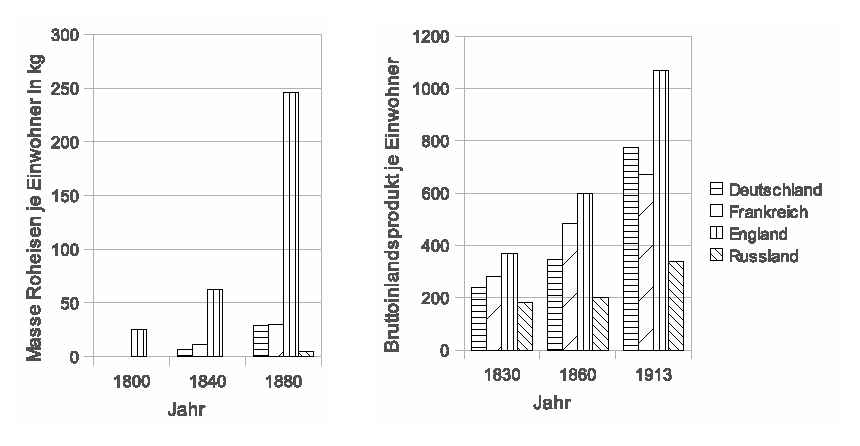
\includegraphics[width=\textwidth]{vorr-gb-diag.eps}
\caption{Roheisenproduktion und Bruttoinlandsprodukt europäischer
Staaten}
\label{pic:vorr-gb-diag}
\end{figure}

\paragraph{Wie Abbildung \ref{pic:vorr-gb-diag} zeigt,} hat
Großbritannien den wirtschaftlichen Entwicklungsprozeß deutlich eher
und mit deutlich höherer Intensität begonnen als andere europäische
Staaten. Es gilt also herauszufinden, wie es zu dieser rasanten
Entwicklung kam.\\

\begin{aufgabe}
Begründen Sie die Vorreiterrolle Englands anhand der besonderen
Voraussetzungen, die dieses Land im Industrialisierungsprozeß
hatte!\footnote{Dazu ist der Inhalt von Abbildung
\ref{pic:vorr-gb-diag} hinreichend}
\end{aufgabe} 

\subsection{Innenpolitische Entwicklung}
\index{Großbritannien!innenpolitisch}

Die \dat{Große Revolution von 1640 bis 1688}
\index{Großbritannien!Große Revolution} \index{Glorious Revolution}
hatte der mittelalterlich"=feudalen Epoche in England ein Ende gesetzt.
Die neue Verfassung sah zensusgebundenes Wahlrecht und
Parlamentssitzvergabe vor und ermöglichte so der \beg{gentry}, den
alten Feudaladel zu verdrängen und ihre fortschrittlichen
wirtschaftlichen Interessen durchzusetzen.

Außerdem sorgte die scharfe Abgrenzung zwischen den Schichten --
Unter-, Oberschicht, Bedienstete etc. -- für eine klare Regelung der
gesellschaftlichen und sozialen Verhältnisse. 


\subsection{Außenpolitische Entwicklung}
\index{Großbritannien!außenpolitisch}

\paragraph{\nam{Henry \Rm{7}} (1486\,--\,1509)} England beginnt eine lange
Tradition der internationalen Seefahrt.

\paragraph{\nam{Elisabeth \Rm{1}} (1558\,--\,1603)} Die englische Flotte
erringt den \dat{Sieg gegen die spanische Armada} und wird so zur
Seemacht. -- Außenhandel und Piraterie weiten sich aus.

\paragraph{\nam{James \Rm{1}} (1603\,--\,1625)} erwirbt 13 Kolonien als
Rohstoffquellen für England und legt so den Grundstein für eine
gezielte Kolonialpolitik.

\paragraph{\Nam{Cromwell, Oliver}{Oliver Cromwell}
(1599\,--\,1658)} England sichert seine Vormachtstellung auf See durch
Siege gegen Holland und Spanien und erwirbt weitere Kolonien, wie zum
Beispiel Jamaika.

\paragraph{\nam{Charles \Rm{2}} (1660\,--\,1685)} Der Krieg gegen
Holland bringt neue Kolonien -- Neuholland und Neuamsterdam.

\paragraph{1714\,--\,1815} Großbritannien erweitert im \dat{War of
Jenkins' Ear 1739\,--\,1742} seinen Kolonialbesitz, erwirbt durch das
Wegfallen Frankreichs als Konkurrenten durch den \dat{Siebenjährigen
Krieg 1756\,--\,1763} Kanada und steigt so endgültig zur Weltmacht
auf.\\

Großbritannien hatte also vor allem durch Handel und Seefahrt einen
gewaltigen Vorrat an Macht, Geld, Rohstoffen, Arbeitern und
Absatzmärkten gewonnen. Dieser bildete die Grundlage für den rasanten
Industrialisierungsprozeß. Abbildung \ref{pic:vorr-gb-gr} bietet
nochmals einen Überblick.

\begin{figure}
\centering
%\begin{sideways}
%\input{vorr-gb-gr.eepic}
%\end{sideways}
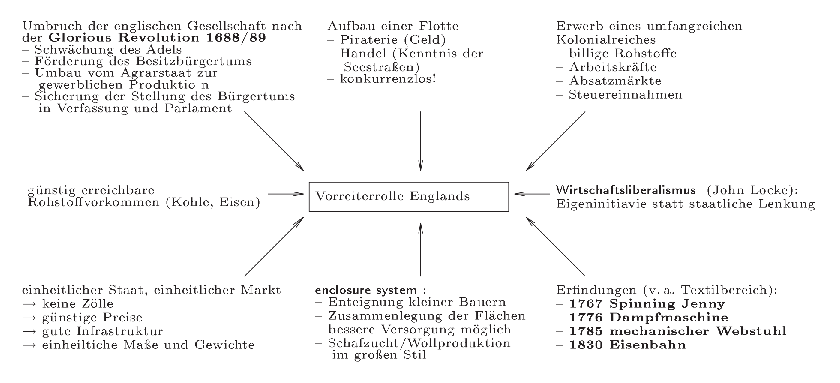
\includegraphics[width=\textwidth]{vorr-gb-gr.eps}
\caption{Ursachen für die Vorreiterrolle Englands}
\label{pic:vorr-gb-gr}
\end{figure}

\endinput

\section{Die Überwindung der Rückständigkeit Deutschlands}
\label{sec:aufh-rueckst-d}
\index{Industrialisierung!Deutschland}

\begin{figure}
\centering
%\begin{sideways}
%\input{vergl-d-e.eepic}
%\end{sideways}
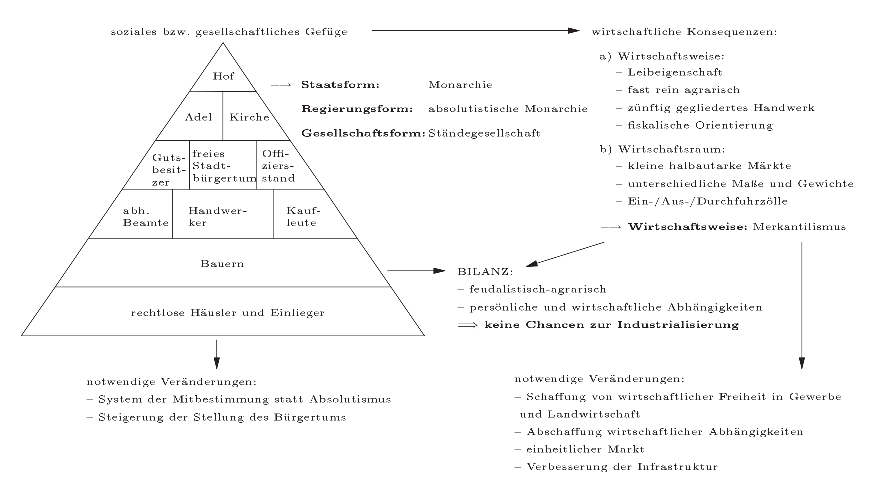
\includegraphics[width=\textwidth]{vergl-d-e.eps}
\caption{Die deutschen Verhältnisse}
\label{pic:dt-verh}
\index{Deutschland!Rückständigkeit}
\end{figure}

\begin{aufgabe}
Zeigen Sie an vier ausgewählten Faktoren, daß Deutschland im
Vergleich zu England als rückständig zu bezeichnen ist!
\end{aufgabe}

\paragraph{Wie Abbildung \ref{pic:dt-verh} zeigt,} waren um 1800
dringend Maßnahmen nötig, um ebenfalls in die industrielle Revolution
einsteigen zu können. Dieser Abschnitt soll zeigen, wie diese
beschaffen waren und was sie bewirkten. \\

\begin{aufgabe}
Stellen Sie an einem Beispiel die Überwindung der Rückständigkeit
Deutschlands im Vergleich zu England dar!
\end{aufgabe}

\subsection[Die Preußischen Reformen]
{Die Preußischen Reformen\footnote{Da die Informationen aus dem im
Geschichtsunterricht gehaltenen Vortrag ungeeignet waren, verwende ich
hier hauptsächlich Material aus \cite{BaswiSchuGesch}.}}
\index{Preußische Reformen}

\mar{Welche Idioten haben damals den Vortrag zu diesem Thema gemacht?}
\begin{aufgabe}
Untersuchen Sie die Preußischen Reformen auf ihre Veränderungen
für das Wirtschaftsgefüge hin!

Fassen Sie sämtliche Informationen zusammen, die zum wirtschaftlichen
Aufschwung Deutschlands als Voraussetzung anzusehen sind und stellen
Sie deren Wirkung dar!
\end{aufgabe}

\paragraph{Nach dem \dat{Krieg gegen Napoleon 1806/1807}} war Preußen
dem Zusammenbruch nahe. Daraufhin initiierten fortschrittliche und
einflußreichende Persönlichkeiten -- allen voran Reichsfreiherr
\Nam{Stein, Karl vom und zum}{Karl vom und zum Stein} und Fürst
\Nam{Hardenberg, Karl August von}{Karl August von Hardenberg} -- eine
Reihe von tiefgreifenden Reformen, die den Wiederaufbau und die
Befreiung des Staates von der französischen Fremdherrschaft
ermöglichen sollten.

Damit einher ging auch eine wirtschaftliche Reform Preußens, dessen
auf dem System der persönlichen Abhängigkeit beruhende Gutswirtschaft
von am Wirtschaftsliberalismus orientierten Grundsätze abgelöst
wurde.

\subsubsection{Bauernbefreiung}
\index{Bauernbefreiung}
\index{Regulierungsedikt}
\index{Oktoberedikt}

Das \dat{Oktoberedikt von 1807} hob die Erbuntertänigkeit und damit
die Leibeigenschaft auf und ermöglichte ihnen den Besitz von eigenem
Land. Die Gutsbesitzer wurden gemäß dem \dat{Regulierungsedikt von
1809} entschädigt.

Der so geschaffene \emph{freie Bauernstand} war nun in den
Wirtschaftsprozeß integriert und also an Produktionssteigerungen
interessiert.

\subsubsection{Städteordnung}
\index{Städteordnung}

Mit der \dat{Einführung der Städteordnung 1808} gewährte Preußen seine
Städten die selbständige Verwaltung ihrer Angelegenheiten. Die Bürger
konnten fortan aktiv und passiv an der an einen niedrigen Zensus
gebundenen Wahl zur Stadtverordnetenversammlung, die
wiederum Magistrat und Bürgermeister (Exekutive) wählte, teil- und
damit auf die Politik Einfluß nehmen.

Dies sind die Ursprünge der kommunalen Selbstverwaltung in Deutschland.

\subsubsection{Verwaltungsreform}
\index{Verwaltungsreform}

Die \emph{Verwaltungsreform} sollte
\textquote[\cite{BaswiSchuGesch}]{einen lestungsfähigen, sparsamen
und bürgernahen Staatsapparat [\dots] schaffen.} Dazu gehörten eine
Vereinfachung der Behördenstruktur durch eindeutige Klärung der
Zuständigkeiten und die Trennung von Justiz und Verwaltung. Möglich
wurde dies durch die neuen Ein"-stel"-lungs- und Laufbahnkriterien für
Beamte (Qualität statt Gunst) und die fortschreitende
Verschriftlichung und Archivierung von Vorgängen. -- Das
Berufsbeamtentum, wie es heute noch fast unverändert in Deutschland
besteht, wurde geprägt. -- Außerdem wurden die Beamten durch relativ
hohe Gehälter bestechungssicher gemacht.\mycite{WikPreusRef}

Ein weiterer bedeutender Inhalt der Verwaltungsreform war die
Schaffung des \emph{klassischen Kabinetts} aus Ministerien (fünf an
der Zahl) mit klar abgegrenzten Ressorts.

\subsubsection{Gewerbereform}
\index{Gewerbereform}

\dat{1810/11 wurde die Gewerbefreiheit} eingeführt. -- Um ein Gewerbe
aufzunehmen genügte der Erwerb eines Gewerbescheins.
\mar{Gewerbe\-steuer? -- Stimmt. Einfügen!} Damit ging die Aufhebung
des Zunftzwangs und somit die Beseitigung zahlreicher Monopole einher.
Dies und die weitgehende Abschaffung der staatlichen Aufsicht über die
Wirtschaft beförderte Konkurrenz und freien Markt.

\subsubsection{Folgen}

\begin{itemize}
\item Unabhängigkeit von den Gutsherren bringt ehemalige Bauern als
Arbeitskräfte in die Städte.
\item zunehmende Bedeutung des Gewerbes auch in ländlichen Gebieten
\item zunehmende Verstädterung
\item später: Verschärfung der sozialen Frage durch übermäßige Zunahme
der Zahl der Handwerker bei starker Konkurrenz
\end{itemize}


%%%%%%%%%%%%%%%%%%%%%%%%%%%%%%%%%%%%%%%%%%%%%%%%%%%%%%%%%%%%%%%%%%%%%%

\subsection{\dat{Die Fr"uhindustrialisierung 1770\,--\,1850}}
\label{ssc:frueh-ind}
\index{Fr"uhindustrialisierung}

\begin{aufgabe}
Stellen Sie Ansätze wirtschaftlichen Aufschwunges in Deutschland
anhand der Frühindustrialisierung dar!

Bewerten Sie die Wirkungsweise dieser auf den
Industrialisierungsprozeß insgesamt!
\end{aufgabe}

\paragraph{Die Verarbeitung von Agrarprodukten} wie sie in
Zuckerfabriken, Branntweinbrennereien, Brauereien, Ölmühlen und
Tabakfabriken betrieben wurde, bildete die Wurzeln des
Unternehmertums. So wurde beispielsweise der Zuckerrübenbauer zum
Zuckerfabrikanten und der Textilverleger zum Textilfabrikanten.

\paragraph{Die Textilproduktion beruhte auf dem Verlagssystem}
(beispielsweise heimgewerbliche Leinenherstellung), das in dieser
Phase der Industrialisierung zur Blüte kam
\mycite[207]{gelbesGeschichts}.  Mit der \dat{Einführung mechanischer
Webstühle 1830} wurden dann die Voraussetzungen für die
Textilindustrie geschaffen.

\paragraph{Ferner erschloß man neue Industriezweige,} wie den
Kohlebergbau und die Erzgewinnung.\\

Diese Ansätze wirtschaftlichen Aufschwungs schufen einen Bedarf nach
Maschinen. -- Kleine Reparaturwerkstätten entwickelten sich zu
Maschinenfabriken. -- Man benötigte Metall. -- Um die isolierten
Produktionsinseln zu verbinden, mußte man die Infrastruktur aufbauen.
-- Man baute 1835 die erste Eisenbahnstrecke. -- Wieder brauchte man
Metall.

Hier zeigen sich die Grundlagen der \beg{Interdependenzen} -- starker
Rückkopplungseffekte, die die folgende rasante Entwicklung
Deutschlands vom Agrar- zum Industriestaat bedingten.

Die Wirtschaft selber entwickelte sich in der Zeit der
Frühindustrialisierung allerdings nur langsam.

%%%%%%%%%%%%%%%%%%%%%%%%%%%%%%%%%%%%%%%%%%%%%%%%%%%%%%%%%%%%%%%%%%%%%%

\subsection{Der Zollverein}
\label{ssc:zollv}
\index{Zollverein}

\begin{aufgabe}
Stellen Sie den Entstehungsprozeß des Zollvereins dar!

Bewerten Sie seine Bedeutung für den Wirtschaftsaufschwung/die
Industrialisierung in Deutschland!
\end{aufgabe}

\subsubsection{Entstehungsprozeß}

\paragraph{Vorläufer:} süddeutscher Zollverein, mitteldeutscher
Handelsverein, preußisch-hessischer Verein

\begin{chronik}
\item[1.\,1.\,1834]
\dat{Zollvereinigungsvertrag} zwischen den Vorläufervereinen -- Der
\emph{deutsche Zollverein} entsteht.

\item[bis 1854]
Westerweiterung durch Anschluß weiterer Länder

\item[1857]
Einführung des Zollvereinstalers

\item[1867]
Norderweiterung

\item[1868]
verbindliche Einführung von \emph{Meter und Kilogramm}
\index{metrisches System}

\item[1871]
Zollverein ist vollständig\footnote{Zur Zusammensetzung des
Zollvereins siehe
\href{http://de.wikipedia.org/wiki/Gebiet_des_Deutschen_Zollvereins}
{diesen Wikipediaartikel}}
\footnote{Österreich wurde trotz Antrages nicht aufgenommen, da das
den Verein dominierende Preußen seine Rivale durch die zusätzlichen
Zahlungen schwächen konnte.}
und umfaßt zur Reichsgründung das gesamte Reichsgebiet
\index{Deutsches Reich}
\end{chronik}


\subsubsection{Politische Bedeutung}

\begin{itemize}
\item ökonomische und materielle Verbindung der Deutschen zu einer
\emph{Nation}
\item Vorbereitung einer echten Nation
\item Stärkung der materiellen Kraft der deutschen Lande durch Wahrung
der auswärtigen Gesamtinteressen
\item Verschmelzung einzelner Provinzialinteressen zu einem
Nationalinteresse -- Erweckung eines Nationalgefühls
\end{itemize}

\subsubsection{Wirtschaftliche Bedeutung}

\begin{itemize}
\item \mar{?} Wiedergeburt des deutschen Unternehmergeistes
\item \mar{?} Teilhabe der deutschen an allen
Nationalangelegenheiten 
\item \mar{?} Anteilnahme des Mittelstandes und der
Großgrundbesitzer an praktischer Politik
\item Grundlage für einheitlichen Markt
\item Wegfall der Zollschranken
\item einheitliche Währung und Maßeinheiten
\end{itemize}

$\Longrightarrow$ Bedingung für ein modernes Wirtschaftssystem


%%%%%%%%%%%%%%%%%%%%%%%%%%%%%%%%%%%%%%%%%%%%%%%%%%%%%%%%%%%%%%%%%%%%%%

\subsection{Der neue Unternehmertypus}
\index{Deutschland!Unternehmertum}

\begin{aufgabe}
Zeigen Sie, daß sich in Deutschland ein neuer Unternehmertypus
Herausbildete und stellen Sie ihn vor!

Begründen Sie, daß er einen Beitrag zur Überwindung der
Rückständigkeit Deutschlands leisten konnte!
\end{aufgabe}

\subsubsection{Entstehung von Unternehmen}

\begin{itemize}
\item Handwerker bauen auf technischen oder finanziellen Grundlagen
oder auf Basis einer Idee Werkstätten zu Fabriken aus.
\item \beg{Feudalunternehmer}
\item Unternehmensgründung auf Basis von Kapitalbesitz oder Erbschaft
(z.\,B. \Nam{Krupp, Alfred}{Alfred Krupp}
\end{itemize}

\subsubsection{Entwicklung zum \emph{neuen} Unternehmer}

Private Unternehmer, Techniker, Kaufleute, Wissenschaftler und
Politiker unternahmen Bildungsreisen nach Großbritannien, von wo sie
Technologien und Anregungen für das deutsche Bildungswesen
mitbrachten. Sie importierten auch britische Maschinen und knüpften
Beziehungen, über welche sie britische Fachleute nach Deutschland
holten.

Hier entwickelte sich eine neue Art, Unternehmen zu gründen: Man
setzte risikofreudig teilweise das gesamte Eigen- oder auch
Familienkapital ein. Wo dieses nicht reichte, schlossen sich mehrere
Unternehmer zusammen -- man gründete Aktiengesellschaften -- oder
wurden Kredite aufgenommen -- Großbanken, wie die \ins{Deutsche Bank}
oder die \ins{Dresdner Bank} entstanden.

\subsubsection{Mitwirkung der Unternehmer bei der Überwindung der
Rückständigkeit Deutschlands}

\begin{description}
\item[Wissen und Erfahrung:] Import von technischen Neuerungen,
Maschinen, Facharbeitern und Ingenieuren
\item[Bildungssystem:] Übergang zu innerdeutscher Ausbildung von
Fachkräften und Ingenieuren an Fachschulen und technischen Hochschulen
\item[Aufschwung des Finanzwesens:] hohe private Investitionen und
damit verbundenes Risiko
\item[technischer Fortschritt:] Kapitalismus führt zu hohem
Konkurrenzdruck -- Unternehmen verbessern eigenständig Produktions-
und Verarbeitungsprozesse. (forschendes Unternehmertum)
\end{description}

Damit war bald sowohl die finanzielle wie auch die technologische
Unabhängigkeit vom Ausland gewährleistet. Die neuen Unternehmer trugen
so maßgeblich zum Aufbau eines wirtschaftlich konkurrenzfähigen
deutschen Kaiserreiches bei.

%%%%%%%%%%%%%%%%%%%%%%%%%%%%%%%%%%%%%%%%%%%%%%%%%%%%%%%%%%%%%%%%%%%%%%

\subsection[Veränderungen in der Infrastruktur]
{Veränderungen in der Infrastruktur \mycite[157/158]{braunesGeschichts}}

\begin{aufgabe}
Weisen Sie nach, daß eine Verbesserung der Infrastruktur in
Deutschland stattgefunden hat!

Bewerten Sie die Bedeutung dessen für den Industrialisierungsprozeß!
\end{aufgabe}

\paragraph{Die Verbesserung der deutschen Infrastruktur} begann in der
Zeit der Frühindustrialisierung: Man befestigte die Landstraßen, baute
Flüsse aus und verband sie durch Kanäle. Dampfschiffe erleichterten
und beschleunigten den den Gütertransport.

\paragraph{Die weitaus bedeutendste Veränderung} war aber die
Einführung der Eisenbahn \index{Eisenbahn} in Deutschland. Nur
sinnvoll durch den Zollverein (\emph{siamesische Zwillinge}) erfuhr
sie seit ihrem \dat{ersten Einsatz 1935} eine rasante
Entwicklung\footnote{Zu konkreten Zahlen siehe
\cite[159]{braunesGeschichts} und \cite{WikEisenbahn}} und wurde zum
entscheidenden Motor der Industrialisierung.

Einerseits erleichterte, beschleunigte und verbilligte sie den
Personen- und Warenverkehr erheblich. Dadurch eröffneten sich nicht
nur neue Möglichkeiten, Rohstoffe zu beschaffen beziehungsweise
Produkte zu vertreiben, sondern förderte ebenso den kulturellen
Austausch und vergrößerte die Anzahl der Arbeiter in Form von
Pendlern.

Andererseits befeuerte die neue riesige Nachfrage nach Stahl für
Schienenverlegung und Eisenbahnherstellung die Schwerindustrie und den
Arbeitsmarkt. Deren Expansion verlangte wiederum nach weiterem Ausbau
der Eisenbahn und so weiter. -- Diese äußerst starke
\beg{Interdependenz} führte in der Folge den sprunghaften Anstieg der
Wirtschaftsmacht Deutschlands.



%%%%%%%%%%%%%%%%%%%%%%%%%%%%%%%%%%%%%%%%%%%%%%%%%%%%%%%%%%%%%%%%%%%%%%

\subsection{Entstehung von Industriegebieten -- Das Ruhrgebiet}
\index{Industriegebiete!Entstehung}
\index{Ruhrgebiet}

\begin{aufgabe}
Zeigen Sie am Beispiel des Ruhrgebietes die schrittweise Entstehung
industrieller Ballungsgebiete!

Bewerten Sie die Bedeutung solcher Ballungsgebiete für den
Industrialisierungsprozeß!
\end{aufgabe}

\subsubsection[Entstehungsprozeß]{Entstehungsprozeß\footnote{Hier am
Beispiel des Ruhrgebiets. -- In anderen Gebieten ähnlich.}}

\begin{enumerate}
\item heranwachsende Stahlindustrie seit 1820 -- Strukturwandel von
Landwirtschaft zu Industrie nach Kohlefunden
\item 1840\,--\,1848 Ausbau von Eisenbahn und Binnenschiffahrt führt
zur Verbesserung der Infrastruktur
\item Übergang vom Stollen- zum Schachtbau
\item Eröffnung von Zechen in großer Zahl führt zu starker Zuwanderung
\item Eisenindustrie ab 1850, forcierte Entwicklung durch Eisenbahnbau
\item 1850\,--\,1870: Kohle!
\item Land- und Intensivwirtschaft zur Versorgung der Bevölkerung in
den Randgebieten der Ballungszentren
\item Nachfolgeindustrien
\end{enumerate}

\subsubsection{Bedeutung der Ballungsgebiete für den
Industrialisierungsprozeß}

\begin{itemize}
\item kein Zoll
\item kürzere Transportwege
\item Zusammenarbeit der Unterhehmen
\item Konzentration von Fachpersonal
\item Konzentration von Wissenschaft und Forschung
\item Investition der Rendite in neue Techniken, Betriebe etc.
\end{itemize}

$\Longrightarrow$ Sprungbrett für die Industrialisierung des gesamten
Landes

\endinput



\chapter{Die \emph{Soziale Frage} und Ansätze für deren Lösung}
\label{chp:soziale-frage}
\index{Soziale Frage}

\begin{aufgabe}
Die Industrielle Revolution wird in der historischen Betrachtung als
Segen und Fluch bezeichnet. Nehmen Sie zu dieser Sichtweise wertend
Stellung! 
\end{aufgabe}

\section{Die Entstehung der Arbeiterschaft als Klasse}
\label{sec:arb-klas-entst}
\index{Arbeiterklasse}

\mar{irgendwie mehr Geographie -- Wo bleiben die Arbeiter?} Ausgehend
von der \dat{Bevölkerungsexplosion ab circa 1800}, deren Ursachen die
Aufhebung der ländlichen Eheverbote, medizinische und
landwirtschaftliche Fortschritte waren und die sich zu einem sich
selbst erhaltenden Prozeß entwickelte, führte die Industrielle
Revolution zu einem \emph{sozialen Wandel}. Dieser schlug sich in der
Herausbildung von Abwanderungs- (vor allem ländliche Regionen wie
Ostpreußen) und Zuwanderungsgebieten (Ballungszentren wie das
Ruhrgebiet) und in der Entstehung von Großstädten und Städten
allgemein nieder.

Dieser Prozeß der \emph{Urbanisierung} ging einher mit der
Herausbildung der Arbeiterklasse, die den Hauptanteil an der
Binnenmigration hatte.

\endinput

\section{Die soziale und gesellschaftliche Lage der Arbeiterschaft
während der Industrialisierung}
\label{sec:soz-ges-lag-arb}
\index{Arbeiterklasse!soz. und ges. Lage}

\subsection{Wohn- und Lebensverhältnisse}

\begin{itemize}
\item Wohnungsknappheit durch rasantes Bevölkerungswachstum
$\Rightarrow$ Bau von \beg{Mietskasernen}:

\begin{itemize}
\item kleinste dunkle feuchte (meist Einraum-) Wohnungen $\Rightarrow$
keine Privatsphäre
\item miserable sanitäre Verhältnisse (eine Toilette für 50 Personen)
\item kaum Heizung
\item Schlafgängertum
\end{itemize}

\item mangelnde Hygiene, Krankheiten, Seuchen
\item Familienväter oft betrunken:

\begin{itemize}
\item Lösung familiärer Konflikte oft mit Gewalt
\item keine Erziehungsinstanz
\item keine Vorbilder für die Heranwachsenden
\end{itemize}

\item schlechte Erziehung und fehlende Schulbildung $\Rightarrow$ kaum
Chancen auf sozialen Aufstieg, Kriminalität
\end{itemize}

\subsection{Arbeitsverhältnisse}

\begin{itemize}
\item Hohe Spezialisierung der Arbeit führte zu Produktivitäts- und
Qualitätssteigerung, aber auch zu Sinnentleerung, Stupidität und
Monotonie.
\item härteste Arbeitsbedingungen
\item hohes Unfallrisiko
\item keine Versicherung
\item kein Kündigungsschutz
\item überlange Arbeitszeiten (bis zu 16 Stunden an sechs Tagen in der
Woche)
\item Hungerlöhne
\item Arbeiterheer führte zu Lohndumping. -- Selbst Kinder mußten
arbeiten.
\end{itemize}

Es entstand also eine neue Zweiklassengesellschaft mit der besitzenden
Klasse, deren Attribute Reichtum, politische und wirtschaftliche Macht
waren, auf der einen Seite und der arbeitenden Klasse, die durch
Massenverelendung und -armut gekennzeichnet war, auf der anderen.

Allerdings muss man dazusagen, dass es auch in der Arbeiterklasse
Standesunterschiede gab. So standen die Facharbeiter, deren äußeres
Kennzeichen der Hut war über den älteren (30\,--\,40 Jahre) und den
jüngeren einfachen Arbeitern. Diese hatten eine Mütze auf dem Kopf.
Auf der untersten Stufe standen die Tagelöhner, die keinerlei feste
Anstellung hatten. Die Entlohnung und die Qualität der
Lebensverhältnisse lief proportional zu dieser Rangordnung. Die Folge
waren starke Spannungen und Uneinigkeit innerhalb dieser
Klasse\footnote{Den Facharbeiter ging es beispielsweise recht gut. Da
sie außerdem Macht über die anderen Arbeiter besaßen, waren sie
verhaßt.} Das behinderte die Arbeiter bei ihrem späteren Kampf für
bessere Lebensverhältnisse und verzögerte die Lösung der sozialen
Frage.

\endinput

\section[Die soziale Frage nach \Nam{}{Hegel}]
{Die soziale Frage nach \Nam{}{Hegel}\mycite{HegelGrundl}}
\label{sec:soz-frag-heg}
\index{Soziale Fragel!nach Hegel}
\Nam{Hegel, Georg Wilhelm Friedrich}{}

Zur Problematik der sozialen Frage nach \Nam{}{Hegel} siehe die Abbildungen
\ref{pic:soz-frag-sch} und \ref{pic:soz-frag-sch-rev}.

\begin{figure}
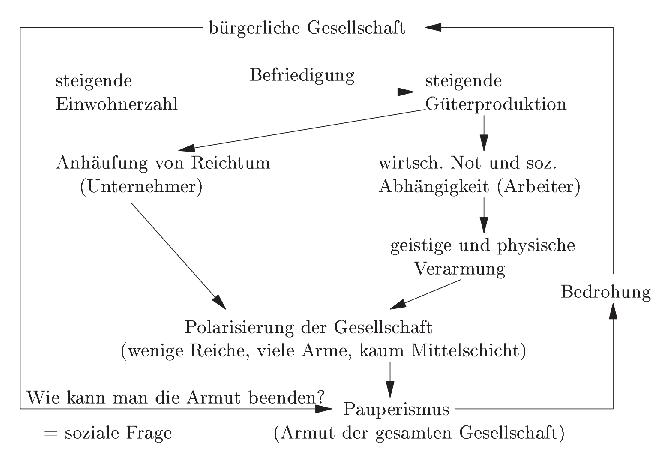
\includegraphics[width=\textwidth]{soz-frag-sch.eps}
\caption{Entstehung der sozialen Frage nach \Nam{}{Hegel}}
\label{pic:soz-frag-sch}
\end{figure}

\begin{figure}
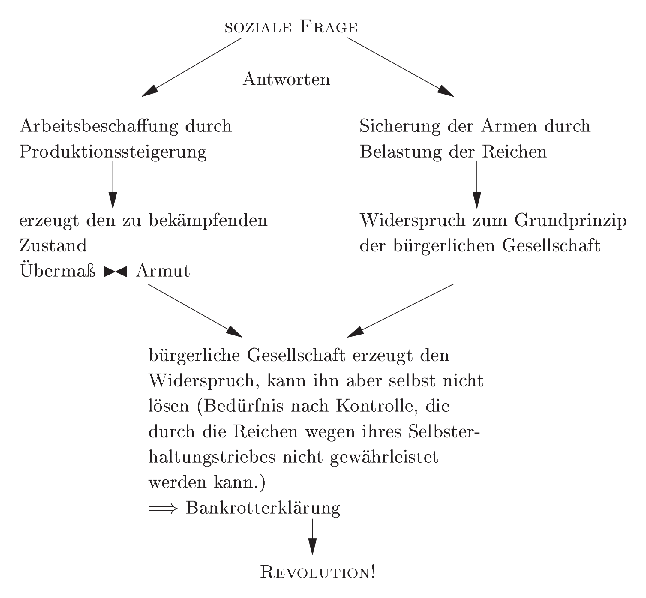
\includegraphics[width=\textwidth]{soz-frag-sch-rev.eps}
\caption{Folgen der sozialen Frage nach \Nam{}{Hegel}}
\label{pic:soz-frag-sch-rev}
\end{figure}

\endinput

\section{Lösungsansätze für die soziale Frage}
\label{sec:soz-frag-loes}
\index{soziale Frage!Lösungsansätze}

\begin{aufgabe}
Stellen Sie einen Maßnahmenkomplex zur Abmilderung/Lösung der Sozialen
Frage vor und prüfen Sie seine Wirksamkeit anhand Hegels Auffassungen! 
\end{aufgabe}

\subsection{Der Marxismus -- Veränderung durch Umbruch}
\label{ssc:marxismus}
\index{Marxismus}
\index{Materialismus}
\mar{\cite{DudPolGes} bietet hier eine gute Darstellung.}

\begin{aufgabe}
Erarbeiten Sie aus der Quelle Marx' Sicht auf die Rolle der
Bourgeoisie in der Geschichte!

Untersuchen Sie die Richtigkeit der fettgedruckten Position anhand des
kapitalistischen Produktionsprozesses in Marx' sogenannter \jar{Basis}! 

Überprüfen sie anhand des Hegelschen Systems der Sozialen Frage,
inwiefern die Ideen Marx' eine Lösung dieser darstellen!
\end{aufgabe}

Im Hefter ist dies in vorerst ausreichender Form dargestellt.

%%%%%%%%%%%%%%%%%%%%%%%%%%%%%%%%%%%%%%%%%%%%%%%%%%%%%%%%%%%%%%%%%%%%%%

\subsection{Die Arbeiterschaft -- Hilfe zur Selbsthilfe}
\label{ssc:arb-bew}
\label{ssc:soz-frag-loes-arb}
\index{Arbeiterbewegung}

\begin{aufgabe}
Untersuchen Sie, inwiefern die Gewerkschaften zur Lösung der sozialen
Frage beitrugen!
\end{aufgabe}

\subsubsection{Ausgangspunkt}

Der Vorteil der Arbeiter war, daß sie eine äußerst breite Schicht der
Bevölkerung bildeten. Unter der Voraussetzung, daß sie sich
zusammenschließen und als die Masse handeln, die sie waren, kann man
ihnen große Chancen, ihre Ziele und Interessen durchzusetzen,
einräumen.

Genau diese Voraussetzung ist aber das Problem, denn die Arbeiter
waren keine homogene Masse. Vielmehr gab es auch hier eine soziale
Schichtung, die sich in der Gehaltsstruktur ausdrückte und zum
ständigen Konflikt beispielsweise zwischen Meistern und
\glq{}Angelernten\grq{} führte. Das ständig bereitstehende
\emph{Ersatzheer} führte zu großer Konkurrenz untereinander. Dieses
Konfliktpotential wurde noch durch die Fabrikordnungen vergrößert,
denn diese sahen Kollektivstrafen vor.

Zur unterschiedlichen sozialen kam noch die unterschiedliche regionale
Herkunft. Da es der Arbeiterschaft an organisatorischem Wissen fehlte,
war es auch hier schwer, eine breite Basis für die Durchsetzung der
Ziele zu finden.

Die Lebensumstände der Arbeiter waren weiterhin schon so miserabel,
dass diese entweder gar keine Zeit fanden, sich um andere Probleme als
ihre eigenen, zu kümmern oder die ständigen Sorgen von vornherein in den
Alkohol oder den Sport flohen.\\


\subsubsection{Entwicklung der Arbeiterbewegung in Großbritannien}
\index{Arbeiterbewegung!Großbritannien}

\begin{chronik}
\item[nach 1814/15] zunehmende Politisierung des Aufbegehrens der
Arbeiter, Streiks

\item[1824] Aufhebung des Koalitionsverbots, Bildung von
Gewerkschaften und Gewerkschaftsverbänden in der Folge

\item[1840] Aus der chartistischen\footnote{Der Name \emph{Chartismus}
leitet sich aus dem Gesetzentwurf ab, der dieser Strömung entstammte
und Forderungen nach beschränkungslosen (Zensus etc.) jährlichen
geheimen allgemeinen Wahlen, Diäten für Abgeordnete und anderem
umsetzen sollte.} Strömung entstand die \ins{National
Chartist} als erste allerdings illegale Arbeiterpartei unserer Zeit.

\item[1860] Nachdem die politische Richtung der Arbeiterbewegung ins
Stocken gekommen war, bildet sich aus den entstehenden \emph{Trade
Unions} (Gewerkschaften) der \ins{Trade Union Council}.

\item[1864] Gründung der \ins{Internationalen
Arbeiterassoziation}\footnote{\Nam{Marx, Karl}{Karl Marx} war
eines der führenden Mitglieder.} (IAA) als Zusammenschluss aller
Arbeiterorganisationen

\item[1876] Auflösung der IAA nach Erfüllung ihrer Aufgabe,
Fortsetzung der Arbeit in Parteien
\end{chronik}


\subsubsection{Arbeiterparteien in Deutschland}
\index{Arbeiterparteien!Deutschland}
\mar{Zur Entwicklung siehe vorerst das Organigramm im Hefter.}

Ziele/Forderungen:

\begin{itemize}
\item Brechung des \Beg{Ehernes Lohngesetz}{Ehernen
Lohngesetzes}\footnote{Da \cite{WiLexEhLohnGes} eine andere Definition
bringt, als ich im Glossar niedergeschriebenen habe, ist fraglich, ob
der hier abgedruckte Sachverhalt stimmt.}
\item allgemeine, gleiche, direkte Wahl (Druckmittel gegen
Unternehmer)
\item Befreiung der Arbeiterklasse durch die Arbeiterklasse
\item Besetitigung der Abhängigkeit des Lohnarbeiters
\item politische Freiheiten (Voraussetzung für ökonomische
Freiheiten)
\item marxistische Strömungen: Revolution \index{Marxismus}
\item politisch-praktische Strömungen: Reformen
\end{itemize}

Mittel:

\begin{itemize}
\item Parteibildung und -arbeit
\item Wahlrechtskämpfe
\item Zusammenschluss von Arbeiterorganisationen
\item Gründung von Arbeiterproduktivgenossenschaften (Vorschlag
\Nam{Lassalle, Ferdinand}{Lassalle}s) -- Arbeiter selbst als
Unternehmer
\item Programme, Zeitschriften
\end{itemize}


\subsubsection{Gewerkschaften in Deutschland\mycite{MustaGeGe}}
\index{Gewerkschaften!Deutschland}

Die deutsche Gewerkschaftsbewegung wies einige Unterschiede zu der in
Großbritannien auf. So wurde in Deutschland durch späte Einführung des
Koalitionsrechts und Sozialistengesetz ein erheblicher Druck ausgeübt.
Dies führte dazu, dass die Vereinigungen im Untergrund
weiterexistieren mussten. Dadurch zu kluger Planung und Organisation
gezwungen, erfuhren die Gewerkschaften eine Stärkung.

Weiterhin waren die deutschen Gewerkschaften ideologisch breiter
aufgestellt. Das bedeutete natürlich, dass alle ihre
Interessenvertretung fanden, hatte aber auch den Nachteil, dass die
Möglichkeiten, als Masse zu handeln, eingeschränkt waren.

Letztendlich legte man in Deutschland sehr großen Wert auf die
organisatorische Trennung zwischen Gewerkschafts- und Parteiarbeit.
-- Die Gewerkschaften übernahmen die überparteiliche soziale
Unterstützung und Basisarbeit während politische und parlamentarische
Arbeit den Parteien zufiel. Man suchte so, die Sorge für die Lage der
Arbeiter unabhängig von politischen Meinungsverschiedenheiten zu
machen, rief die Arbeiter aber gleichzeitig auf, durch Parteieintritt
den Einfluss des Proletariats auf das Staatsgeschehen zu
vergrößern.\mycite{ResErfGeKo} \mycite{ResKonfGeVoGo}\\

\noindent Entwicklung:

\begin{chronik}
\item[nach 1848/49] lokale Arbeiterkomitees und -zusammenschlüsse

\item[1868] Gründung des \Ins{Allgemeiner Deutscher
Arbeiterschaftsverband}{Allgemeinen Deutschen
Arbeiterschaftsverbandes}

\item[1868] Gründung der \Ins{}{\Nam{Hirsch, Max}{Hirsch}-\Nam{Duncker,
Franz}{Duncker}schen-Gewerksverbände}\footnote{\cite{LEMOHiDu} datiert
hier auf 1869.}

\item[1869] Gründung der \Ins{Internationale
Gewerksgenossenschaften}{Internationalen Gewerksgenossenschaften}
durch \Nam{Bebel, August}{August Bebel} und \Nam{Liebknecht,
Wilhelm}{Wilhelm Liebknecht}

\item[1869] Koalitionsfreiheit für Preußen

\item[1878] \ges{Gesetz gegen die gemeingefährlichen Bestrebungen der
Sozialdemokratie} -- Weiterexistenz im Untergrund

\item[1886] Streikerlass in Preußen -- Verfolgung illegaler
Gewerkschaften

\item[1890] Aufhebung des Sozialistengesetzes

\item[1890] Gründung der \ins{Generalkommission der Freien
Gewerkschaften Deutschlands} als erster Dachorganisation für
sozialistische Gewerkschaften auf Initiative von \Nam{Legien,
Carl}{Carl Legien}

\item[1891] Gründung des \Ins{Deutscher
Metallarbeiterverband}{Deutschen Metallarbeiterverbandes} -- erste
Industriegewerkschaft

\item[1890er] Gründung christlicher Gewerkschaften, Formierung zum
Verband \mar{Irgendwie stimmen hier einige Zahlen nicht.}
\end{chronik}

Ziele:

\begin{itemize}
\item soziale Ziele --Loslösung von politischen Fragestellungen
\item kürzere Arbeitszeit
\item höhere Löhne
\item Abbau der Frontstellung des Proletariats gegen das Bürgertum
(Hirsch-Duncker)
\item Förderung und Wahrung der Würde und des materiellen Interesses
der Arbeiter
\end{itemize}

Mittel:

\begin{itemize}
\item Streik
\item lokale Komitees und Arbeiterzusammenschlüsse $\longrightarrow$
Gewerkschaften $\longrightarrow$ Gewerkschaftsverbände
\item Presseorgane
\item Kassen zur Unterstützung von Arbeitslosen, Not leidenden,
Kranken, Invaliden, Alten, Wandernden
\end{itemize}

\newpage
%%%%%%%%%%%%%%%%%%%%%%%%%%%%%%%%%%%%%%%%%%%%%%%%%%%%%%%%%%%%%%%%%%%%%%

\subsection{Die Rolle der Unternehmer}
\label{ssc:soz-frag-loes-unt}

\subsubsection{Maßnahmen}

% Breite der ersten Spalte der Tabelle
\newlength{\frstcol}
\settowidth{\frstcol}{\textsc{Harkort}}
\addtolength{\frstcol}{1ex}

% Breite der zweiten und dritten Spalte der Tabelle
\newlength{\sndthrdcol}
\newlength{\wholecols} % Breite von zweiter und dritter Spalte zusammen
\setlength{\wholecols}{\textwidth}
\addtolength{\wholecols}{-\frstcol}
\addtolength{\wholecols}{-5\tabcolsep}
\setlength{\sndthrdcol}{0.5\wholecols}



\tablefirsthead{
\toprule
Untern. & fürsorglicher Charakter & unterdrückender Charakter \\
\midrule}
\tablelasttail{\bottomrule}

\begin{supertabular*}{\textwidth}%
{p{\frstcol}p{\sndthrdcol}p{\sndthrdcol}}
\vspace{0.01pt}
\Nam{Stumm-Halberg, Carl Ferdinand Freiherr von}{Stumm}
& \begin{tablist}
\item Schulen
\item Verantwortlichkeit für außerfabrikale Arbeiterhandlungen
\item Ausschluss von Kinderarbeit
\item niedrigvermietete Werkswohnungen
\item Bibliotheken, Park für die Arbeiter, Militärkapellen
\item Kantinen, Teuerungszulagen
\item Bestrafungs- und Entlassungserlaubnis
\item Sprechstunden für die Belegschaft
\item überdurchschnittliche Löhne
\item protektorale Betriebsverfassungen
\end{tablist}
\noindent $\Longrightarrow$ Schutz der Arbeiter
& \begin{tablist}
\item Heiratserlaubnis nach Eigenschaften und Gesundheit der Partner,
Vorbeugung von Arbeitsausfall während Schwangerschaften
\item Erziehungsüberwachung
\item Zwang zum Kirchenbesuch
\item Arbeiter als geborene Untertanen (\emph{König Stumm})
\index{König Stumm}
\end{tablist}
\noindent $\Longrightarrow$ Eindringen in das Privatleben
\\

\vspace{0.01pt}
\Nam{Krupp, Alfred}{Krupp}
& \begin{tablist}
\item überdurchschnittliche Löhne
\item Betriebskrankenkasse
\item Sterbegelder an Hinterbliebene
\item Werkswohnungen
\item Arbeiterpensionskasse -- Altersabsicherung
\item \ins{Gemeinschaft der Kruppianer} -- Stammbelegschaft
\end{tablist}
& \begin{tablist}
\item Nutzung des \beg{Ersatzheeres}
\item Entlassung als Druckmittel
\item Entlassung bei Parteihörigkeit
\item Betäubung von sozialdemokratischen und gewerkschaftlichen
Bestrebungen
\item leistungsabhängige Entlohnung
\item Strafgelder
\item Beitrittspflicht zur Betriebskrankenkasse
\end{tablist}
\\

\vspace{0.01pt}
\Nam{Harkort, Friedrich}{Harkort}
& \begin{tablist}
\item betriebsinterne Sparkassen -- Sicherung von Grunderwerb
\item Bildungssystem für Kinder und Erwachsene -- geistliche,
sittliche und staatsbürgerliche Bildung seiner Angestellten
\item Ablehnung von Kinderarbeit
\end{tablist}
&\vspace{0.01pt} keine klassische Unterdrückung
\\
\end{supertabular*}

\ \\

Ein weiteres bedeutendes Unternehmen, in dem man die Lage der Arbeiter
zu bessern versuchte, war \ins{Carl Zeiss Jena}. Dabei waren die
dortigen Maßnahmen einmal und auch völlig andere als bei den oben
Aufgeführten.

\endinput



\chapter[Fortentwicklung der Industrialisierung in der ersten Hälfte
des 20. Jh.] {Fortentwicklung der Industrialisierung in der ersten
Hälfte des 20. Jahrhunderts}
\label{chp:fortentw-indust}

\section{Neue gesellschaftliche Schichtung}
\label{neue-ges-schicht}
\index{Gesellschaft}
\index{Agrargesellschaft}
\index{Industriegesellschaft}
\index{Dienstleistungsgesellschaft}

Die Gesellschaft in Deutschland entwickelte sich seit dem \dat{Ende der
Agrargesellschaft 1850} über die Industriegesellschaft zur
\dat{Dienstleistungsgesellschaft ab 1990}.

Dabei kann man drei große Linien erkennen: \emph{Urbanisierung}
\index{Urbanisierung}, \emph{Trennung von Arbeit und Leben}
beziehungsweise Hausgemeinschaft und Arbeitsstätte und eine zunehmende
\emph{Differenzierung der Arbeitnehmergesellschaft} in \beg{Arbeiter}
und \beg{Angestellte}. Außerdem setzte um 1900 die Bürokratisierung
ein. \index{Bürokratisierung} 

\endinput

\section{Neue Leitsektoren}
\label{sec:neue-leits}
\index{Leitsektor}

\subsection[Chemische Industrie]{Chemische Industrie\footnote{Die
Grundlage dieses Abschnitts ist ein schnell im Rahmen des Unterrichts
im Internet recherchierter Kurzvortrag. Da dieses Thema weniger
relevant ist, beschränke ich mich bei der Literatur auf die
Wikipedia-Artikel \cite{WikChemInd}, \cite{WikFarbst}, \cite{WikHaBoVerf}, \cite{WikStaudi} und \cite{WikSteikohteer}.}}
\label{ssc:chem-ind}
\index{Chemische Industrie}

\mar{Warum galt die chemische Industrie in jener Zeit als Friedens-
und damit Staatserhaltend?}
In der ersten Hälfte des 19. Jahrhunderts wurden Verfahren erfunden,
den bei der Gasherstellung anfallenden \emph{Steinkohlenteer}
\index{Steinkohlenteer} nutzbringend zu verwenden. Die neuen Produkte
-- allen voran \emph{Anilin} und \emph{Phenol}
\index{Anilin}\index{Phenol} -- waren Grundstoff für zahlreiche
Synthesen. -- Damit war der Aufstieg der Farbenindustrie eingeleitet.

Es wurden Möglichkeiten gefunden, Medikamente, Düngemittel und
Sprengstoffe künstlich herzustellen. Dadurch konnten bisher unheilbare
Krankheiten geheilt und die landwirtschaftliche Produktion erheblich
gesteigert werden. -- Gesundheits- und Versorgungszustand der
Bevölkerung verbesserten sich erheblich, sodass auch die Nachfrage
nach den immer vielseitigeren Produkten der chemischen Industrie
stieg.

Die enge Kooperation dieses Industriezweigs mit technischen
Hochschulen verbesserte das Bildungssystem und trieb die Forschung
voran. So kam es zu weiteren bedeutenden Erfindungen:

\dat{1910} wurde das \dat{\emph{\Nam{Haber, Fritz}{Haber}-\Nam{Bosch,
Carl}{Bosch}-Verfahren}} \index{Haber-Bosch-Verfahren} erfunden,
welches die Synthese von Ammoniak ermöglichte. Dieser dient als
Grundlage für Sprengstoffe und Kunstdünger. Die Verfügbarkeit neuer
Düngemittel bewirkte neue Forschungen in der Landwirtschaft.

\dat{1922} stellte \Nam{Staudinger, Hermann}{Hermann Staudinger} die
These auf, dass Polymere aus Makromoleküle bestehen und begründete
damit die Polymerchemie. Dies führte zur \dat{großtechnischen
Produktion zahlreicher Kunststoffe ab 1930} (beispielsweise
Polystyren, Polyvinylchlorid, Nylon, Buna). Die \dat{1925 gegründete}
\beg{IG Farben} war hier marktführend.

%%%%%%%%%%%%%%%%%%%%%%%%%%%%%%%%%%%%%%%%%%%%%%%%%%%%%%%%%%%%%%%%%%%%%%

\subsection[Elektroindustrie]{Elektroindustrie\footnote{Dieser und die
folgenden vier Abschnitte entstammend Kurzvorträgen, die ich nicht
selbst gehalten habe und deswegen auch keine Quellen angeben kann.}}
\label{ssc:el-ind}
\index{Elektroindustrie}

\begin{chronik}
\item[ab 1900]
erste kommerzielle Sende- und Empfangsanlagen

\item[1904]
erste Röhrendiode -- Gleichrichtung\index{Röhrendiode}

\item[1906]
erste Triode -- Grundlage für Radio und andere Unterhaltungselektronik 
\index{Triode}

\item[1926\,--\,1931] Entwicklung des Fernsehens\index{Fernsehen}

\item[1900\,--\,1950] auch international marktbeherrschende Stellung
von \beg{AEG} und \beg{Siemens}

\item[1931]
Erfindung des Elektronenmikroskops\index{Elektronenmikroskop}

\item[1941]
Erfindung des Computers (Z\,3)\index{Computer}\index{Z\,3}
\end{chronik}

Diese Entwicklungen läuteten des Computer- und Informationszeitalter
ein: Die neuen Möglichkeiten erweckten sofort großes in der
Bevölkerung, in der Politik und beim Militär, sodass sich die Anzahl
der Arbeitsplätze von \dat{80\,000 Beschäftigten 1900} bis \dat{1950
auf 650\,000} steigerte.

%%%%%%%%%%%%%%%%%%%%%%%%%%%%%%%%%%%%%%%%%%%%%%%%%%%%%%%%%%%%%%%%%%%%%%

\subsection{Fahrzeugbau}
\label{ssc:fahrzbau}
\index{Fahrzeugbau}

Sich aus dem Waggonbau entwickelnd erfuhr dieser Industriezweig in
Folge der \dat{Forderung \Nam{Hitler, Adolf}{Hitler}s} nach einem
Wagen für breite Schichten \dat{1934} großen Aufschwung. So wurde
\dat{1937} die \dat{\ins{Gesellschaft zur Vorbereitung der Deutschen
Volkswagen mbH} gegründet}, \dat{1938 in \ins{Volkswagen GmbH}}
umbenannt.

Das Werk wurde im gleichen Jahr in \ort{Wolfsburg}
errichtet.\index{VW} Es war äußerst günstig gelegen: In der Mitte
Deutschlands mit Anbindung an Autobahn, Eisenbahn und durch den
Mittellandkanal ebenfalls an Wasserstraßen. Außerdem waren Stahlwerke,
beispielsweise in \ort{Salzgitter} nicht fern. Im Krieg leisteten hier
20\,000 Kriegsgefangene und KZ-Insassen Zwangsarbeit.
\index{Zwangsarbeit}

Bei der Produktion des neu entwickelten
\emph{KdF-Wagens}\index{KdF-Wagen}, heute als \emph{VW Käfer}\index{VW
Käfer} bekannt, orientierte man sich am
\emph{Fließbandbetrieb}\index{Fließbandproduktion}, wie er bei
\ins{Ford} in \ort{Detroit} praktiziert wurde. Das neue Auto konnte
vier Personen transportieren, war zuverlässig, einfach reparierbar und
billig. So konnte man die Wirtschaft ankurbeln und die Verwendung beim
Militär war auch möglich.  Im Krieg stand dann auch die
Rüstungsproduktion im Vordergrund.  \index{Rüstung}

Nach dem Krieg war das VW-Werk der britischen Militärregierung
\index{Militärregierung} unterstellt, die die Umstellung auf
Zivilproduktion veranlasste.

\endinput

\section{Fließbandarbeit}
\label{ssc:fliessbarb}
\index{Fließbandarbeit}

Die Arbeitswelt in der ersten Hälfte des 20. Jahrhunderts war geprägt
vom \beg{Taylorismus}, der in Kombination mit dem Fließbandbetrieb die
Massenproduktion ermöglichte.

Dieses neue Prinzip der Trennung von geistiger und körperlicher Arbeit
half bei der Lösung sozialer Probleme und versprach \jar{Wohlstand für
alle}. Der anfängliche Enthusiasmus wich aber bald der
Unzufriedenheit: Durch die Monotonie der Arbeit stellten sich
gesundheitliche Probleme ein. Außerdem konnten sich die Arbeiter nun
kaum noch mit ihrem Betrieb und den Erzeugnissen identifizieren, weil
sie das Endprodukt kaum noch zu Gesicht bekamen.

Die Qualität litt und die Motivation fehlte. Es kam zu Konflikten mit
den Arbeitgebern; wo es möglich war wanderten die Arbeitnehmer in den
Dienstleistungssektor ab.

\endinput

\section{Arbeitsbedingungen in der ersten Hälfte des 20. Jahrhunderts}
\label{sec:arb-bed-20jh}

Die Arbeitswelt in der ersten Hälfte des 20. Jahrhunderts war auch
geprägt von miserablen Arbeitsbedingungen: \emph{Niedrige
Mindestanforderugen}, \emph{fehlende Aufstiegschancen}, 
\emph{hohe Fluktuation}, \emph{niedrige Löhne} und \emph{geringe
Arbeitsplatzsicherheit} machten den Arbeitern das Leben schwer.

Doch man tat auch einiges, um jene Bedingungen zu verbessern.  Gab es
um \dat{1900} wenigstens einige \dat{Herbergen für Wanderarbeiter},
brachte das \dat{\emph{\Nam{Stinnes, Hugo}{Stinnes}-\Nam{Legien,
Carl}{Legien}-Abkommen} vom 15.\,11.\,1918} große Fortschritte. Der
aus Furcht vor einer Vergesellschaftung der deutschen Industrie im Zuge
der Novemberrevolution zwischen Gewerkschafts- \Nam{}{Legien} und
Industrievertretern \Nam{}{Stinnes} geschlossene Vertrag legte die
Zusammenarbeit von Arbeitnehmern und -gebern fest. Die Arbeitgeber
verpflichteten sich so, die Rolle der Gewerkschaften als Vertreter der
Arbeiterinteressen anzuerkennen und sie als gleichberechtigte
Tarifpartner zu betrachten. Außerdem wurde der \emph{Achtstundentag}
bei vollem Lohnausgleich eingeführt.
\index{Arbeitnehmer}
\index{Arbeitgeber}
\index{Gewerkschaft}
\index{Tarifverhandlung}
\index{Achtstundentag}

Damit wurden ab 1918/1919 in allen Branchen \emph{Tarifverträge},
Regelung der Arbeitsbedingungen durch \emph{Kollektivvereinbarungen},
Anerkennung der \emph{Koalitionsfreiheit} durch die Arbeitgeber und
\emph{Arbeiterausschüsse} in Betrieben mit mindestens 50 Beschäftigten
möglich.
\index{Tarifvertrag}
\index{Kollektivvereinbarung}
\index{Koalitionsfreiheit}
\index{Arbeiterausschuss}

\endinput



\chapter[Ursprung und Umsetzung liberaler, nationaler und
kons. Ideen im 19. Jh.]{Ursprung und Umsetzung liberaler und
nationaler sowie konservativer Ideen im 19. Jahrhundert\footnote{Ich
stütze mich bei der Strukturierung dieses Kapitels ausnahmsweise kaum
auf den Hefter, da dort keine erkennbare Struktur existiert.}}
\label{chp:lib-nat-kons}

Dieses Kapitel soll folgende Fragen beantworten:

\textbf{Warum kommt es zur Revolution?}

\textbf{Welche Forderungen haben die Bürger?}

\textbf{Warum haben die Bürger gerade diese Forderungen?}

\section{Die Epoche der Aufklärung}
\label{sec:aufkl}
\index{Aufklärung}

Die Ideen der Aufklärung bildeten die Grundlage für die politischen,
ökonomischen und sozialen Entwicklung, die schließlich zur Revolution
von 1848 führten. Sie beeinflussten außerdem seit Mitte des 18.
Jahrhunderts das Denken aller Menschen in Europa und Nordamerika und
sind bis heute gültig und wirksam.

Dieser Abschnitt soll einen kurzen Überblick über die für das Weitere
relevanten Aspekte der Aufklärung geben.


\subsection{Konflikt mit der alten Ordnung}

% wieder mal Spaltenbreiten berechnen

\begin{tabularx}{\textwidth}{XcX}
\toprule
Situation in Deutschland vor 1815 &
&
Ziele der Aufklärung \\

\midrule
\vspace{-45mm}
\begin{tablist}
\item absolutistische Monarchie 
\item Ständegesellschaft
\item territorialstaatlicher Absolutismus -- Vielzahl von
Einzelstaaten
\item Leibeigenschaft (Bindung als Person)
\item Schollenbindung (Bindung als Pacht)
\item Zünfte/Gilden
\end{tablist}
&
\unitlength=2.5mm
\begin{picture}(3,19)
\thicklines
\put(2,18){\line(-2,-9){2}}
\put(0,9){\line(3,1){3}}
\put(3,10){\vector(-2,-9){2}}
\end{picture}
&

\vspace{-45mm}
\begin{tablist}
\item Vernunftorientierung 
\item gegen Dogmatik der Kirche
\item mündiger Bürger
\item geistige und persönliche Freiheit
\item Toleranz (Religionstoleranz)
\item politisches Mitspracherecht
\end{tablist}
\\

\bottomrule
\end{tabularx}

%%%%%%%%%%%%%%%%%%%%%%%%%%%%%%%%%%%%%%%%%%%%%%%%%%%%%%%%%%%%%%%%%%%%%%

\subsection{Leistungen}

Zu einer sehr komprimierten Übersicht über die Leistungen der
Aufklärung siehe Tabelle \ref{tab:leist-aufkl}.

% angenehme Breite der ersten Spalte
\settowidth{\tymin}{\textbf{Natur-}}

\begin{sidewaystable}
\label{tab:leist-aufkl}
\caption{Leistungen der Aufklärung}
\footnotesize
\renewcommand{\arraystretch}{1.5}

\begin{tabulary}{\textheight}{LLLL}
\toprule

&
\textbf{Die alte Ordnung} &
\textbf{Die Ideen der Aufklärung} &
\textbf{Anwendung der neuen Erkenntnisse} \\

\midrule

\textbf{Naturwissenschaft} &
Spekulation \newline
Überlieferung &
empirische Methode (\Nam{Newton, Sir Isaac}{Newton}): Beobachtung --
Verallgemeinerung bzw. Experiment -- Erkenntnis \newline
einzige Grundlage: \emph{Vernunft} &
\Nam{Newton, Sir Isaac}{Newton}: Gravitationsgesetz \newline
\Nam{Kepler, Johannes}{Kepler}: Gesetze der Planetenbewegung \newline
\Nam{Watt, James}{Watt}: Dampfmaschine \newline
Diese und zahlreiche weitere Erfindungen bringen großen technischen
Fortschritt. Wissenserweiterung und Bildung gewinnen an Bedeutung.
\\

\textbf{Gesellschaft} &
Ständegesellschaft &
natürliche Freiheit und Gleichheit der Menschen (\Nam{Locke,
John}{John Locke}) &
Formulierung der Menschenrecht \\

\textbf{Religion} &
Gott und die Bibel als alleinige Autorität &
von Gott nach vernünftigen Gesetzen geschaffene Welt \newline
Religionsfreiheit &
Toleranz zwischen den Religionen \\

\textbf{Politik} &
Gottesgnadentum -- Absolutheitsanspruch des Herrschers &
Kontrolle des Herrschers durch die Bürger (\Nam{Montesquieu, Baron
de}{Montesquieu}, \Nam{Rousseau, Jean-Jacques}{Rousseau}) &
Gewaltenteilung, demokratische Verfassung, Volkssouveränität \\

\textbf{Wirtschaft} &
staatlich gelenkte Wirtschaft &
Wohlstand aller Bürger des Staates durch wirtschaftliche Freiheit des
Einzelnen (\Nam{Smith, Adam}{Smith}) &
Wirtschaftsliberalismus \\

\bottomrule 
\end{tabulary}
\end{sidewaystable}

%%%%%%%%%%%%%%%%%%%%%%%%%%%%%%%%%%%%%%%%%%%%%%%%%%%%%%%%%%%%%%%%%%%%%%

\subsection{Philosophen der Aufklärung}

Es gab zahlreiche Philosophen, die die Ideen der Aufklärung
entwickelten und verfolgten, darunter zum Beispiel \Nam{Leibniz,
Gottfried Wilhelm}{Leibniz}, \Nam{Kant, Immanuel}{Kant}, \Nam{Herder,
Johann Gottfried}{Herder}, \Nam{Lessing, Gotthold Ephraim}{Lessing}.
Im Folgenden wird jedoch nur Einblick in die Philosophie zweier Männer
gegeben, die sich besonders mit Staatstheorien beschäftigt haben und
deshalb für dieses Kapitel relevant sind.


\subsubsection{\Nam{Montesquieu, Baron de}{Charles de Secondat, Baron
de Montesquieu}}
\index{Gewaltenteilung}
\index{Legislative}
\index{Exekutive}
\index{Judikative}
\index{politische Freiheit}

\Nam{}{Montesquieu} geht in seinem Werk \emph{Vom Geist der
Gesetze}\mycite{VomGeistderGes} unter anderem auf die Frage ein, wie
ein Staat gestaltet sein muss, damit die politische Freiheit der
Bürger gewährleistet ist. Dabei definiert er \jar{politische Freiheit}
als \textquote{jene geistige Beruhigung, die aus Überzeugung
hervorgeht, die jedermann von seiner Sicherheit hat}.

Er stellt dazu fest, dass es in jedem Staat drei Gewalten gibt, die
wir heute \emph{Legislative} (Erlassen von Gesetzen), \emph{Exekutive}
(Umsetzung öffentlicher Beschlüsse) und \emph{Judikative}
(Verhandlung von Streitfällen und Verbrechen). Um also die politische
Freiheit des Bürgers zu sichern, ist es essentiell, dass jene Gewalten
personell strikt voneinander getrennt werden:

\SetBlockThreshold{0}
\blockquote[{\mycite[216\,f.]{VomGeistderGes}\,\footnote{Der
Quellenverweis gilt auch für den obigen Abschnitt.} }]{Alles wäre
verloren, wenn ein und derselbe Mann beziehungsweise die gleiche
Körperschaft entweder der Mächtigsten oder der Adligen oder des Volkes
folgende drei Machtvollkommenheiten ausübte: Gesetze erlassen,
öffentliche Beschlüsse in die Tat umsetzen, Verbrechen und private
Streitfälle aburteilen.}


\subsubsection{\Nam{Rousseau, Jean-Jacques}{Jean-Jacques Rousseau}}
\index{Grundrechte}
\index{Menschenrechte}
\index{Französische Revolution}

\blockquote{Der Mensch wird frei geboren, und dennoch liegt er in
Ketten.}

\blockquote[{\mycite{DerGesVertr}\,\footnote{Ich beziehe mich in
diesen Zitaten und in den folgenden Ausführungen auf den mir
vorliegenden Text. Dieser ist allerdings aus verschiedenen Teilen des
Werkes zusammengestückelt und weder mit Auslassungsmarken, noch mit
einer Quellenangabe versehen. Mit \cite{DerGesVertr} ist damit ein
Hinweis auf eine Volltextfassung gegeben, die allerdings im Wortlaut
nicht exakt meinem Text entspricht.}}]{Auf seine Freiheit verzichten,
heißt auf seine Eigenschaft als Mensch, auf die Menschenrechte, sogar
auf seine Pflichten zu verzichten.}

Wie man an diesen Zitaten erkennen kann, legt \Nam{}{Rousseau}
besonders großen Wert auf Freiheit. Deshalb setzt er auf seiner Suche
nach einer Gesellschaftsform, die Person und Eigentum eines jeden
schützt, also Grund- und Menschenrechte garantiert, die Prämisse, dass
der Mensch in dieser Gesellschaft den gleichen Grad an Freiheit
genießt, wie außerhalb\footnote{Das ist im
\emph{Naturzustand}\index{Naturzustand}}.  Das Ergebnis von
\Nam{}{Rousseau}s Überlegungen ist der \ges{Gesellschaftsvertrag},
welcher die Voraussetzungen erfüllt und den Rahmen für die
Zusammensetzung der Gesellschaft festlegt: Jedes Mitglied der
Gemeinschaft gibt sich mit all seinen Rechten an die Gesellschaft hin.

Inwiefern diese Auffassung utopisch beziehungsweise realistisch ist,
ist eine andere Frage. Dennoch sind die Ideen, die \Nam{}{Rousseau}
hier formuliert, essentiell und waren eine äußerst wichtige geistige
Grundlage für die \emph{Französische Revolution}.


\subsubsection{Zusammenfassung: Wesentliche Ordnungsvorstellungen der
Aufklärer}
\index{Gewaltenteilung}
\index{Volkssouveränität}
\index{Grundrechte}
\index{Menschenrechte}

\begin{enumerate}
\item  das Prinzip der \emph{Gewaltenteilung}, das die Trennung von
ausführender und gesetzgebender Gewalt sowie die Sicherung einer
unabhängigen Rechtssprechung vorsieht
\item das Prinzip der \emph{Volkssouveränität}, das das Recht zur
Gesetzgebung den Vertretern des Volkes vorbehält
\item die Bindung des Gesetzgebers an allgemein gültige \emph{Grund-
und Menschenrechte}
\end{enumerate}

%%%%%%%%%%%%%%%%%%%%%%%%%%%%%%%%%%%%%%%%%%%%%%%%%%%%%%%%%%%%%%%%%%%%%%

\subsection{Umsetzung der Ideen der Aufklärung in der
\index{Französischen Revolution}}
\index{Bürgerrechte}
\index{Menschenrechte}
\index{Grundrechte}

\mar{Siehe Blatt mit schicken Unterstreichungen aus
dem Hefter.}
Während der die \dat{\ges{Erklärung der Bürger- und Menschenrechte}
von 1789} und in die \dat{französischen Verfassungen}, deren erste
\dat{1791} verabschiedet wurde, flossen zahlreiche Ideen der
Aufklärer, insbesondere \Nam{Montesquieu, Baron
de}{Montesquieu}s und \Nam{Rousseau, Jean-Jacques}{Rousseau}s ein. Die
Französische Revolution wiederum hatte großen Einfluss auf die
politischen Entwicklungen in Deutschland, die in diesem Kapitel
behandelt werden.

\endinput

\section[Nationale und liberale Bewegungen]{Nationale und liberale
Bewegungen\mycite{19Jh1}}
\label{sec:nat-lib-bew}
\index{nationale Bewegungen}
\index{liberale Bewegungen}

\mar{Belege aus IzpB?}
\subsection{Befreiungskriege gegen \Nam{Napol\'eon \Rm{1}}{Napol\'eon}}
\index{Befreiungskriege}
\index{Napol\'eonische Kriege}
\index{Nationalromantik}
\index{Nationalismus}
\index{Franzosenhass}

\mar{Muss das genauer gewusst werden?}
Der Begriff \emph{Befreiungskriege} steht hier für die Kriege
vornehmlich der von \Nam{}{Napol\'eon} besetzten Länder gegen die
französische Fremdherrschaft in der Zeit zwischen dem \dat{Rückzug der
\emph{Grande Arm\'ee} aus Russland 1812} und der \dat{Abdankung des
Kaisers 1814}. Jene Erfahrungen, die des gemeinsam geführte Krieges
und der Fremdherrschaft, waren eine wichtige Wurzel der
nationalen Bewegung, deren Formen von Nationalromantik bis zum
radikalen Nationalismus reichten. Ein verbreitetes Symptom war auch
der teils extreme Hass auf Franzosen.


\subsubsection{Ausgangslage}

Der \dat{Russlandfeldzug} und die
einhergehende Niederlage der Grande Arm\'ee hatten \dat{1812} Napol\'eon
gewaltige Verluste eingebracht.  Dadurch fasste Europa neuen Mut, eine
Befreiung von der französischen Herrschaft zu versuchen.


\subsubsection{Erhebung Preußens}

\begin{chronik}
\item[30.\,12.\,1812]
Unterzeichnung der \ges{Konvention von Tauroggen} als
preußisch-russisches Neutralitätsabkommen -- Anfang vom Ende der
erzwungenen militärischen Unterstützung Frankreichs durch Preußen

\item[28.\,2.\,1813]
Unterzeichnung des \Ges{Bündnis von Kalisch}{Bündnisses von Kalisch}
durch \nam{Wilhelm \Rm{3}} -- Zusammenarbeit Preußens und Russlands
für die Befreiung Europas

\item[10.\,3.\,1813]
erstmalige Verleihung des \emph{Eisernen Kreuzes} \index{Eisernes
Kreuz} durch Wilhelm \Rm{3}

\item[16.\,3.\,1813]
Kriegserklärung Preußens an Frankreich

\item[17.\,3.\,1813]
Aufruf \ges{An Mein Volk} von Wilhelm \Rm{3}\mycite{AnMeinVolk}
\end{chronik}


\subsubsection{Frühjahrsfeldzug 1813}
\index{Antinapoleonische Koalition}

\begin{chronik}
\item[2. und 20. Mai]
Schlachten bei \ort{Großgörschen} und \ort{Bautzen} -- Siege Napol\'eons

\item[12. Juli]
\emph{Trachenbergplan} \index{Trachenbergplan} -- gemeinsame Strategie
Preußens, Russlands und Schwedens gegen Napol\'eon

\item[11. August]
Kriegserklärung Österreichs an Frankreich. Zuvor waren Österreich,
Schweden und Großbritannien der Koalition gegen Napol\'eon beigetreten.
Deren Ziele waren die vollständige \emph{Wiederherstellung}
Österreichs und Preußens, die \emph{Unabhängigkeit} aller deutschen
Staaten sowie die Auflösung des \ins{Rheinbund}es.\footnote{Ich
vermute, dass das in dem Handout des Vortrags, der dieses Thema
behandelte, so gemeint war.}
\end{chronik}


\subsubsection{Herbstfeldzug 1813}

\dat{Ende August 1813} stießen drei russisch-schwedisch-preußische
Armeen unter österreichischem Oberbefehl gegen Napol\'eon vor:
\ins{Nordarmee} und \ins{Schlesische Armee} bei \ort{Dresden} und die
\ins{Hauptarmee} in \ort{Böhmen}.\footnote{Zumindest soweit ich das
Handout verstehe.}


\subsubsection{Weitere Schlachten 1813}
\index{Alliierte!Napol\'eonische Kriege}

\begin{chronik}
\item[23. Aug.] \ort{Großbeeren} -- Sieg der Alliierten
\item[26. Aug.] \ort{Katzbach} -- Sieg der Alliierten
\item[26./27. Aug.] \ort{Dresden} -- Sieg Napol\'eons
\item[20. Aug.] \ort{Kullm} und \ort{Nollendorf} -- Sieg der
Alliierten
\item[6. Sept.] \ort{Dennewitz} -- Sieg der Alliierten
\end{chronik}

In der Folge kündigte auch Bayern das Bündnis mit Napol\'eon und trat
der Koalition bei, was die Auflösung des Rheinbundes einleitete.

Mit der Umzingelung Napol\'eons bei \ort{Leipzig} kam es schließlich zur
\emph{Völkerschlacht}.


\subsubsection{Völkerschlacht bei Leipzig}
\index{Völkerschlacht}

Napol\'eon hatte sich mit stark geschwächtem Heer und knapper Munition
bei Leipzig aufgestellt. Die am \dat{16. Oktober 1813} beginnende
Schlacht verlief für die Alliierten erfolgreich. Der Sieg brachte den
Verlust des Rheinbundes und den Zusammenbruch der französischen
Herrschaft über Deutschland.

Da Napol\'eon jedoch am \dat{19. Oktober} rechtzeitig den
\dat{Rückzug} einleitete, konnte ein großer Teil seiner Armee
entkommen.


\subsubsection{Untergang Napol\'eons}

Die Alliierten marschierten nun in Frankreich ein und nahmen
\dat{\ort{Paris} am 31. März 1814}. Napol\'eon dankte ab und ging ins
Exil. Der \dat{\ges{Frieden von Paris} vom 30. Mai 1814} brachte das
vorläufige Ende der Napol\'eonischen Kriege.

%%%%%%%%%%%%%%%%%%%%%%%%%%%%%%%%%%%%%%%%%%%%%%%%%%%%%%%%%%%%%%%%%%%%%%

\subsection{Ausgangslage am Anfang des 19. Jahrhunderts}

War Deutschland bis 1871 keine Nation, existierte vor der
napol\'eonischen Besatzungszeit lediglich eine Vielzahl (über 100)
kleiner bis winziger Territorialstaaten. Zu einer Milderung dieses
Zustandes kam es durch Erscheinungen der \emph{Industrielle
Revolution}, durch \Nam{Napol\'eon \Rm{1.}}{Napol\'eon} selbst und im
Zuge der Befreiung von der französischen Fremdherrschaft:


\subsubsection[Veränderungen durch die Industrielle
Revolution]{Veränderungen durch die Industrielle Revolution (siehe
auch \ref{sec:aufh-rueckst-d})}

\begin{itemize}
\item Zollvereine: \ins{Allgemeiner deutscher Zollverein},
\ins{Zollvereinstaler}
\item Verbesserung der Infrastruktur (bspw. Eisenbahn) 
\item einheitlicher Markt
\end{itemize}


\subsubsection{Veränderungen durch
Napol\'eon\mycite[244-246]{gelbesGeschichts}}
\label{sss:veraend-nap}
\index{Flurbereinigung}
\index{Kleinstaaterei!Ende}

\begin{enumerate}
\item \emph{Flurbereinigung}:
Nachdem die linksrheinischen Fürsten ihre \dat{1801 Gebiete an
Frankreich abtreten} mussten, wurden sie durch den
\dat{\ges{Reichsdeputationshauptschluss} 1803} mit Land aus der von
Napol\'eon betriebenen \beg{Säkularisation} und \beg{Mediatisierung}
entschädigt.

\item \dat{Mediatisierung zahlreicher Reichsritterschaften 1805}

\item \dat{Gründung des \Ins{}{\beg{Rheinbundes}} 1806}:
In dieser Verwaltungseinheit von 16 deutschen Staaten führte Napol\'eon 
den \ges{Code civil} ein. Diese Gesetzessammlung galt bereits in
Frankreich, brachte liberale Reformen mit sich und bildete eine sich
über die Rheinbundstaaten erstreckende einheitliche Gesetzesgrundlage.
\end{enumerate}


\subsubsection{Veränderungen im Zuge der Befreiung von Napol\'eon}
\mar{Wo sind sie denn?}

%%%%%%%%%%%%%%%%%%%%%%%%%%%%%%%%%%%%%%%%%%%%%%%%%%%%%%%%%%%%%%%%%%%%%%

\subsection[Der Wiener Kongress 18. September 1814\,--\,9. Juni
1815]{Der Wiener Kongress 18. September 1814\,--\,9. Juni
1815\mycite[80\,--\,84, 88/89]{braunesGeschichts}\,\mycite[252\,--\,254]{gelbesGeschichts}}
\index{Wiener Kongress}
\index{Aufklärung}
\index{Nationalbewusstsein}

\begin{aufgabe}
Bewerten Sie anhand der Prinzipien den Charakter des Wiener
Kongresses! 
\end{aufgabe}

In deutschen Landen hatte sich während der Zeit der naol\'eonischen
Herrschaft einiges getan: Im \emph{territorialen Bereich} gab es
Veränderungen der Länder, der Grenzen und der Fürstentitel, in der
\emph{Wirtschaft} hatte sich der Markt vereinheitlicht und
\emph{politisch} gab es noch mehr Zündstoff: Die \emph{Aufklärung}
(siehe auch \ref{sec:aufkl} Griff um sich, die Befreiungskriege hatten
Anfänge eines \emph{Nationalbewusstseins} geschaffen und einige
Staatsleute begannen, der Entwicklung mit \emph{Reformen} beizukommen.

Um mit den Ereignissen Schritt zu halten, trafen sich 200 Vertreter
vieler europäischer Länder nach dem vorläufigen Sieg über Napol\'eon
in \ort{Wien} zu einem Kongress unter dem Vorsitz des \Nam{Metternich,
Klemens Wenzel Lothar von}{Fürsten von Metternich}.

Unter den zentralen Prinzipien

\begin{center}
\Large
%\begin{tabularx}{0.75\textwidth}{ccc}
%\textbf{\beg{Legitimität}} & \textbf{\beg{Solidarität}}
% & \textbf{\beg{Restauration}} 
%\end{tabularx}
\end{center}

\noindent berieten sie über die \emph{Neuregelung} europäischer
Grenzen und damit verbundenen territorialen \emph{Ausgleich}, über die
\emph{Fixierung} der Niederlage Frankreichs, politische
\emph{Regulierung} und ein europäisches
\emph{Sicherheitssystem}.\index{Sicherheitssystem} Damit einher ging
die Festsetzung der \emph{Pentarchie}, also die Voherrschaft der fünf
europäischen Großmächte Frankreich, Großbritannien, Österreich, Preußen 
und Russland in Europa.\index{Pentarchie}

An seinen Prinzipien eindeutig erkennbar, war der Wiener Kongress ein
Rückschritt in Bezug auf die nationale und liberalen Bemühungen in
deutschen Landen, wobei diese noch kaum begonnen hatten.

%%%%%%%%%%%%%%%%%%%%%%%%%%%%%%%%%%%%%%%%%%%%%%%%%%%%%%%%%%%%%%%%%%%%%%

\subsection{Nationale Bewegung}
\index{nationale Bewegungen}
\index{Einheit!19. Jahrhundert}
\index{Nationalstaat}

\noindent Wurzeln:

\begin{itemize}
\item die \emph{Französische Revolution}\index{Französische
Revolution} -- Die Leistungen, die die Menschen hier durch ihren
Patriotismus gebracht hatten, besonders natürlich die großen Erfolge
des materiell und personell Unterlegenen französischen Heeres, hatte
große Vorbildwirkung auf Deutschland.

\item die \emph{Preußischen Reformen} (siehe auch
\ref{sec:aufh-rueckst-d}) -- Sie erhöhten in den Befreiungskriegen
Kampfmoral und Bereitschaft zum Kampf und nährten die Hoffnung auf
einen Nationalstaat.

\item \Nam{Napol\'eon \Rm{1}}{Napol\'eon} als \emph{der} Übermittler
des Nationalbewusstseins -- das sich letztlich gegen ihn richtete.

\item Französische Fremdherrschaft und Ablehnung des
\jar{Franzosentums} betreiben die Bildung einer deutschen Identität.

\item der Aufruf \Nam{Wilhelm \Rm{3}}{Wilhelms \Rm{3}} \ges{An Mein
Volk}\mycite{AnMeinVolk}
\end{itemize}


\noindent Ziel:
\index{Kleinstaaterei!Ende}

Das zentrale Ziel der nationalen Bewegung war natürlich die Einheit
Deutschlands. Diese war zwar durch den \ins{Zollverein} (siehe
\ref{ssc:zollv} im wirtschaftlichen Bereich gegeben und Napol\'eon
hatte durch seine Flurbereinigung (siehe \ref{sss:veraend-nap})
der Kleinstaaterei ein Ende gesetzt. Dennoch konnte man nicht von
Deutschland als einem \emph{Nationalstaat} sprechen.


%%%%%%%%%%%%%%%%%%%%%%%%%%%%%%%%%%%%%%%%%%%%%%%%%%%%%%%%%%%%%%%%%%%%%%

\subsection{Liberale Bewegung}
\index{liberale Bewegungen}
\index{Gewaltenteilung}
\index{Volkssouveränität}
\index{Grundrechte}
\index{Menschenrechte}
\index{Gottesgnadentum!Abschaffung}

\noindent Ursprung:
\index{Gleichheit}
\index{Freiheit}
\index{Staatstheorie}
\index{Vertragstheorie}
\index{Gesellschaftsvertrag}
\index{Privateigentum}

Die Grundlage der liberalen Bewegungen war die bereits in Abschnitt
\ref{sec:aufkl} besprochene Aufklärung, die bekanntlich die Vernunft
ganz vornanstellt und an ihr Erkenntnis und Handeln bemisst. Über
diese gelangten dann auch die großen Vertrags- beziehungsweise
Staatstheoretiker \Nam{Locke, John}{John Locke}, \Nam{Montesquieu,
Baron de}{Baron de Montesquieu} und \Nam{Rousseau,
Jean-Jacques}{Jean-Jacques Rousseau}  mit ihren Ansätzen
genannt:\footnote{Natürlich gehört zu diesen auch \Nam{Hobbes,
Thomas}{Thomas Hobbes}. Doch dieser hat mit zur liberalen einer eher
unbedeutende Beziehung.} zu den Prinzipien, die auch zu den Prinzipien
der liberalen Bewegung wurden:

\begin{itemize}
\item Einführung eines Gesellschaftsvertrages zur eindeutigen
Festlegung der Rechte und Pflichten der Bürger und der Regierung eines
Landes und als Begründung beziehungsweise Legitimierung der Herrschaft
des regierenden Personenkreises -- kein \emph{Gottesgnadentum}
\item Volkssouveränität
\item Gewaltenteilung
\item Sicherung des Privateigentums
\item natürliche Gleichheit und Freiheit des Individuums
\item angeborene, unantastbare und unveräußerliche Grund- und
Menschenrechte
\end{itemize}


\noindent Zentrale Ziele:
\index{Feudalismus!Abschaffung}
\index{Wirtschaft!freie}
\index{Merkantilismus!Abschaffung}
\index{Wahl}

\begin{itemize}
\item Abschaffung der feudalen Gesellschaftsordnung 
\item Begrenzung der Fürstenmacht durch Verfassungen -- Anerkennung
von Grund- und Menschenrechten, Gewaltenteilung
\item Mitwirkung der Bürger durch gewählte Vertreter an der
Staatslenkung
\item freie Wirtschaft
\end{itemize}

Für die Erreichung dieser Ziele waren durch den \ges{Code civil} im
Rheinbund und die Reformen in Preußen zumindest Ansätze vorhanden.

%%%%%%%%%%%%%%%%%%%%%%%%%%%%%%%%%%%%%%%%%%%%%%%%%%%%%%%%%%%%%%%%%%%%%%

\subsection{Freiheit und Einheit}
\index{Französische Revolution}

Natürlich bildeten Anhänger der liberalen und nationalen Bewegung
nicht unterschiedliche Lager. Vielmehr entwickelten sich in immer
größeren Teilen der Bevölkerung Forderungen nach \emph{Freiheit und
Einheit}. Dies waren auch die Ideen der Französischen Revolution
gewesen, die dort umgesetzt worden waren und dann durch die
Eroberungskriege \Nam{Napol\'eon \Rm{1}}{Napol\'eon}s nach Deutschland
getragen wurden.

\subsubsection{Burschenschaften}
\index{Burschenschaften}

Die hauptsächlichen Träger solcher Ideen waren in Deutschland die
\emph{Burschenschaften}. \dat{1817} formulierten
sie ihre \dat{\emph{Grundsätze}}\mycite{GrundsBursch} -- sowohl
nationale als auch liberale Ziele und Forderungen, deren letztere hier
zusammenfassend genannt werden sollen: \\

\noindent konstitutionell:
\begin{itemize}
\item Gewählte Vertreter erlassen Gesetze
\item Alle höheren Ämter müssen sich vor dem Volk verantworten.
\item Die Fürst führt den Willen des Volkes aus. 
\end{itemize} 

\noindent wirtschaftlich:\\
Schaffung eines einheitlichen Marktes durch Abschaffung von Zöllen,
Einführung einheitlicher Maße und Gewichte etc.\\

\noindent sozial:
Freiheit und Gleichheit generell und vor dem Gesetz \\

Diese Forderungen standen natürlich den Auffassungen der Restauration
und des Wiener Kongresses entgegen. Deshalb wurden mit den
\dat{\ges{Karlsbader Beschlüsse}n 1819} scharfe Restriktionen
eingeführt (siehe \ref{ssc:kampf-lib-res}).


\subsubsection{Vormärz in der Literatur}
\index{Vormärz!Literatur}

Während neben den Burschenschaften nur kleine Teile der Bevölkerung
aktiv die Ideale Freiheit und Einheit verfolgten, entwickelte sich in
der Literatur rasch die Strömung des \emph{Vormärz}. -- Dichter wurden
zum Sprachrohr der Bewegung und zum Stimmungsbarometer. Daher sollen
hier Auszüge aus drei Gedichten der damaligen Zeit Beachtung finden.

Derer Erstes stammt von \Nam{Körner, Theodor}{Theodor Körner} und
damit aus der Zeit der Befreiungskriege\index{Befreiungskriege}:

\poemtitle*{\Nam{}{Theodor Körner} (1791\,--\,1813): Aufruf
(1813)\mycite{KoernerAufr}}
\settowidth{\versewidth}{Frisch auf, mein Volk! – Die Flammenzeichen rauchen,}

\begin{verse}[\versewidth]
Frisch auf, mein Volk! Die Flammenzeichen rauchen, \\
Hell aus dem Norden bricht der Freiheit Licht. \\
Du sollst den Stahl in Feindes Herzen tauchen; \\
Frisch auf, mein Volk! – Die Flammenzeichen rauchen, \\
Die Saat ist reif – ihr Schnitter, zaudert nicht! \\
Das höchste Heil, das letzte, liegt im Schwerte! \\
Drück' dir den Speer ins treue Herz hinein! – \\
Der Freiheit eine Gasse! – Wasch' die Erde, \\
Dein deutsches Land, mit deinem Blute rein! \\
\mbox{[\dots]}
\end{verse}


\poemtitle*{\Nam{Herwegh, Georg}{Georg Herwegh} (1817\,--\,1875):
Aufruf (1814)\mycite{HerweghAufr}}
\settowidth{\versewidth}{Spricht er wohl den Segen drein.}

\begin{verse}[\versewidth]
\mbox{[\dots]} \\
Reißt die Kreuze aus der Erden! \\
Alle sollen Schwerter werden, \\
Gott im Himmel wird's verzeihn. \\
Hört er unsre Feuer brausen \\
Und sein heilig Eisen sausen, \\
Spricht er wohl den Segen drein. \\
\mbox{[\dots]}
\end{verse}

Das Gedicht, aus dem der folgende Auszug stammt, bezieht sich auf den
\dat{Aufstand der schlesischen Weber 1844} (siehe
\ref{ssc:kampf-lib-res}). Das Wort \jar{Fluch} in der vierten
Zeile bezieht sich auf Gott, König und falsches Vaterland, die in den
vorhergehenden Strophen verflucht werden:

\poemtitle*{\Nam{Heine, Heinrich}{Heinrich Heine} (1797\,--\,1856):
Die schlesischen Weber (1847)\mycite{HeineWeber}}
\settowidth{\versewidth}{Altdeutschland, wir weben dein Leichentuch,}

\begin{verse}[\versewidth]
\mbox{[\dots]} \\
Das Schiffchen fliegt, der Webstuhl kracht, \\
Wir weben emsig Tag und Nacht -- \\
Altdeutschland, wir weben dein Leichentuch, \\
Wir weben hinein den dreifachen Fluch -- \\
\vin Wir weben, wir weben!\flq \\
\end{verse}

Heine war übrigens den Auswüchsen des Nationalismus gegenüber
recht kritisch eingestellt, wie in seinem Kommentare über das
Wartburgsfest und seine Zeit in einer \Ort{Göttingen}{Göttinger}
Burschenschaft zeigen:

\blockquote{Auf der Wartburg hingegen herrschte jener unbeschränkte
Teutomanismus, der viel von Liebe und Glaube greinte, dessen Liebe
aber nichts anderes war als Haß des Fremden und dessen Glaube nur in
der Unvernunft bestand, und der in seiner Unwissenheit nichts Besseres
zu erfinden wußte, als Bücher zu verbrennen!}

\blockquote[{\mycite{HeineBursch}}]{Im Bierkeller zu Göttingen musste
ich einst bewundern, mit welcher Gründlichkeit meine altdeutschen
Freunde die Proskriptionslisten anfertigten, für den Tag, wo sie zur
Herrschaft gelangen würden. Wer nur im 7. Glied von einem Franzosen,
Juden oder Slawen abstammte, ward zum Exil verurteilt. Wer nur im
mindesten etwas gegen Jahn oder überhaupt gegen altdeutsche
Lächerlichkeiten geschrieben hatte, konnte sich auf den Tod gefasst
machen\dots}



%%%%%%%%%%%%%%%%%%%%%%%%%%%%%%%%%%%%%%%%%%%%%%%%%%%%%%%%%%%%%%%%%%%%%%

\subsection{Politisierung der Bewegung}

\begin{table}
\caption{Anzahl und Charakter der Volksunruhen in Deutschland}
\label{tab:volksunr}

\newcolumntype{Y}{>{\centering}X}
\newcolumntype{Z}{>{\raggedright}X}
\newlength{\studlength}
\settowidth{\studlength}{Studenten/}
\newlength{\sozlength}
\settowidth{\sozlength}{sozioöko-}

\begin{tabularx}{\textwidth}{lYYYY|Y}
\toprule

&
\parbox{\studlength}{Studenten/\\Universität}\vspace{0.5ex} &
Religion &
Politik &
\parbox{\sozlength}{sozioöko-\\nomisch} &
Summe \\

\midrule

1816\,--\,29 &
13 &
9 &
4 &
3 &
29 \\

1830\,--\,39 &
13 &
20 &
72 &
28 &
133 \\

1840\,--\,47 &
5 &
17 &
33 &
103 &
158 \\

\midrule
Summe &
31 &
46 &
109 &
134 &
320 \\

\bottomrule 
\end{tabularx}
\end{table}

Wie Tabelle \ref{tab:volksunr} zeigt, gewannen \dat{ab 1830
politische Unruhen} deutlich an Dominanz. Sie bewirkten die Ausweitung
politischer Arbeit beziehungsweise politischen Interesses auf breitere
Bevölkerungsschichten. Die politischen Probleme wurden zwar im Zuge
der Industriellen Revolution\index{Industrielle Revolution} von
sozioökonomischen überdeckt. Doch diese vergrößerten ebenso das
Ursachenfeld für eine eventuelle Revolution, die dadurch natürlich
wahrscheinlicher wurde.


\subsubsection{Charakter der Ziele von Liberalen und Demokraten}
\index{Republik}
\index{parlamentarische Monarchie}
\index{Revolution}
\index{Reform}

Demokraten und Liberale vertraten unterschiedliche Ansichten in Bezug
auf die Neugestaltung des Staates. Wie im sogenannten \ges{Offenburger
Programm}\mycite{OffenbProg} deutlich wird, zielten die Demokraten auf
die Errichtung einer Republik oder parlamentarischen Monarchie ab.
Dabei hat ihre Schrift einen einigermaßen revolutionären Charakter.

Die Liberalen suchten mit ihrem \ges{Heppenheimer
Programm}\mycite{HeppProg} jedoch
eher nach Veränderungen auf der bestehenden Rechtsbasis. -- Man
erkennt den reformerischen Charakter.


\subsubsection{Demokratisches und restauratives Prinzip}

\begin{aufgabe}
Erklären sie wesentlich Unterschiede zwischen dem demokratischen und
dem restaurativen Prinzip! 
\end{aufgabe}

\noindent demokratisches Prinzip:
\index{demokratisches Prinzip}

\begin{itemize}
\item Gesetzte werden vom Volk oder Volksvertretern erlassen.
\item Gewaltenteilung
\item Gleichheit aller vor dem Gesetz
\item Gewährung persönlicher Freiheiten (Presse-, Meinungsfreiheit,
\dots) 
\end{itemize}

\noindent restauratives Prinzip
\index{restauratives Prinzip}

\begin{itemize}
\item Stützung der absolutistischen Monarchie
\item alle Macht beim Fürsten -- Verantwortung nur vor Gott
\item Einschränkung persönlicher Freiheit
\item keine Macht im Volk 
\end{itemize}

\endinput

% Ziel: Freiheit nach außen und Selbstbestimmung nach innen

\section{Die Revolution von 1848}
\label{sec:rev-1848}
\index{Revolution!März 1848}

\subsection{Kampf zwischen Liberalismus und Restauration -- Der Weg
zur Revolution}
\label{ssc:kampf-lib-res}

\begin{aufgabe}
Weisen Sie nach, dass die Entwicklung im Zeitraum zwischen 1815 und
1848 in eine Revolution führen musste!
\end{aufgabe}

\begin{figure}
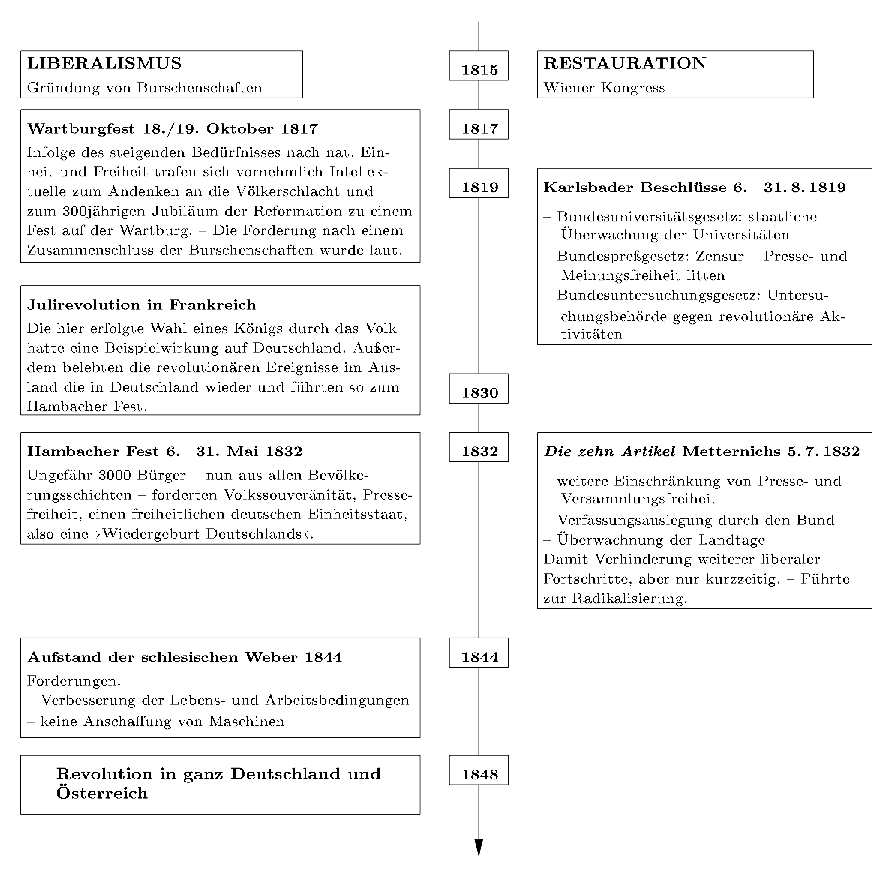
\includegraphics[width=\textwidth]{kampf-lib-rest.eps}
\caption{Das Ringen zwischen Liberalismus und Restauration}
\label{pic:kampf-lib-rest}
\end{figure}

Abbildung \ref{pic:kampf-lib-rest}\footnote{Die \ges{Zehn Artikel}
\Nam{Metternich, Klemens Wenzel Lothar von}{Metternichs} sind in
\cite{ZehnArt} zu finden, weitere Literatur in
\cite[106]{braunesGeschichts}. Die Quellen zu den übrigen Ereignissen
sind mir nicht bekannt.} zeigt die wichtigsten Ereignisse auf dem Weg
zur Revolution von 1848. Man erkennt, dass die Intensität von
antirestaurativen und restaurativen Maßnahmen immer weiter zunahm.
Weiter befeuert wurde die entwicklung durch die sich in Folge der
Industriellen Revolution verschärfenden soziale Lage.

%%%%%%%%%%%%%%%%%%%%%%%%%%%%%%%%%%%%%%%%%%%%%%%%%%%%%%%%%%%%%%%%%%%%%%

\subsection{Ursachenfeld}

\renewcommand*{\arraystretch}{1.5}
\newcolumntype{Y}{>{\setlength{\hsize}{0.55\hsize}\raggedleft}X}
\newcolumntype{Z}{>{\setlength{\hsize}{0.45\hsize}\raggedright}X}
\begin{tabularx}{\textwidth}{Y@{\quad$\lightning$\quad}Z}
restaurative Bewegung   & liberale Bewegung     \\
Absolutismus            & Aufklärung            \\
Industrielle Revolution -- Reichtum
                        & soziale Mißstände -- Armut    \\
territorialstaatlicher Absolutismus
                        & Einheitsbestrebungen
\end{tabularx}

%%%%%%%%%%%%%%%%%%%%%%%%%%%%%%%%%%%%%%%%%%%%%%%%%%%%%%%%%%%%%%%%%%%%%%

\subsection{Anlass}

Begünstigt durch die \dat{Krisenjahre 1847/48} in Frankreich mit
Missernten und Hungerunruhen kam es dort zur
\emph{Februarrevolution}\index{Februarrevolution}. Die Ereignisse in
Frankreich nahm man sich dann in Deutschland zum Vorbild und begann
die Revolution, die schon lange auf ihren Ausbruch gewartet hatte.
\mar{Germania und Bedeutung/Entwicklung von Symbolen.}

%%%%%%%%%%%%%%%%%%%%%%%%%%%%%%%%%%%%%%%%%%%%%%%%%%%%%%%%%%%%%%%%%%%%%%

\subsection{Verlauf}

\begin{figure}
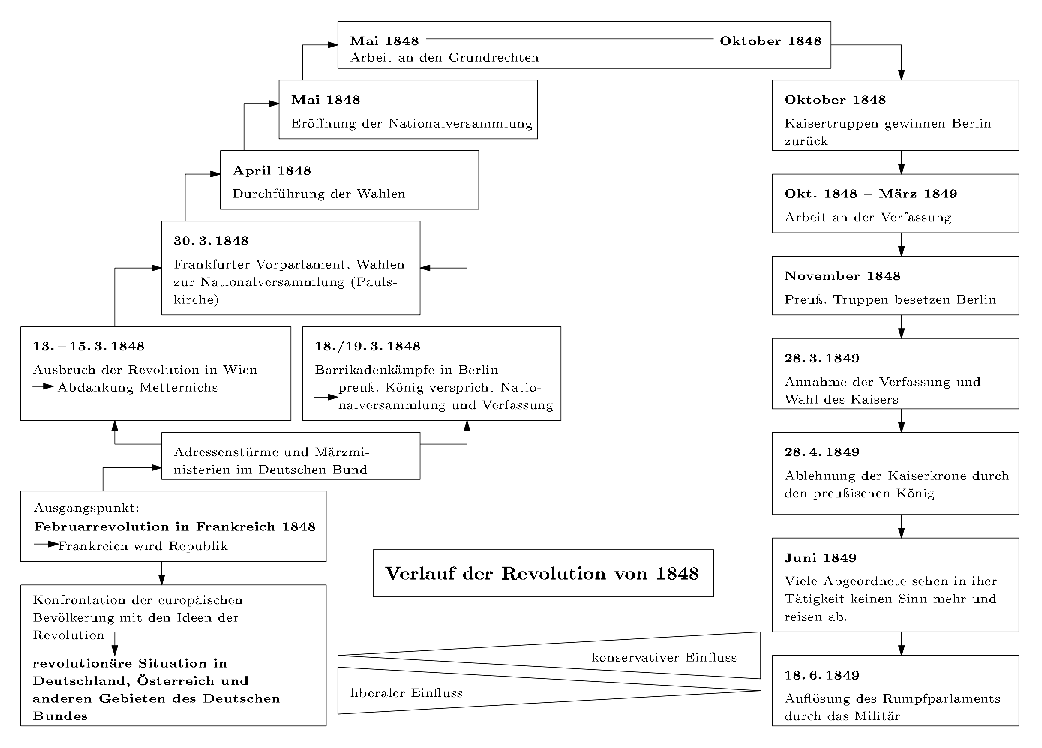
\includegraphics[height=\textwidth, angle=90]{verlauf-rev.eps}
\caption{Verlauf der Revolution von 1848}
\label{pic:verlauf-rev}
\end{figure}

Abbildung \ref{pic:verlauf-rev} bietet einen Überblick über den
Verlauf der Revolution. Diesen kann man in drei Etappen einteilen:
\mar{Richtige Benennung der Phasen?}

Die erste Phase war von kämpferischen Handlungen geprägt. Mit dem
Zusammentritt des \emph{Frankfurter Vorparlaments}
\index{Vorparlament!Frankfurt} begann eine Phase der Machtfestigung.
Der Niedergang setzte in der sehr langen Zeit der \emph{Arbeit an den
Grundrechten} ein. Diese Verzögerung der Vorgänge war nämlich einer
der Gründe für das Scheitern der Revolution: Durch die Uneinigkeit und
die fehlende parlamentarische Erfahrung, dauerte die Komprmissfindung
sehr lange. Das entstehende Machtvakuum nutzten die restaurativen
Kräfte für die Reaktion.

%%%%%%%%%%%%%%%%%%%%%%%%%%%%%%%%%%%%%%%%%%%%%%%%%%%%%%%%%%%%%%%%%%%%%%

\subsection{Verfassungsarbeit}

\begin{aufgabe}
Erläutern Sie die wesentlichen Aufgaben, die die
Paulskirchenversammlung zu lösen hatten und bilanzieren Sie die
jeweilige Lösung! 
\end{aufgabe}

\subsubsection{Parlament}

Das Parlament tagte in der runden
\Ort{Paulskirche!Frankfurt}{Frankfurter Paulskirche}\index{Frankfurt}.
Die 812 Männer unter dem Vorsitz des Liberalen \Nam{Gagern, Heinrich
von}{Heinrich von Gagern} waren hauptsächlich Bildungsbürger und
keinerlei Arbeiter. Man nannte die Versammlung daher auch
\jar{Parlament der Intellektuellen}.


\subsubsection{Grundrechte}
\index{Grundrechte}

Der erste Schwerpunkt der zukünftigten Verfassung für Deutschland
waren die Grundrechte. Auf Basis der Forderungen der Liberalen wurde
so ein umfangreicher Grundrechtskatalog beschlossen und im
\ort{Dezember 1848 angenommen}.


\subsubsection{Grenzen}

Eine sehr umstrittene Frage, die die Verhandlungen stark in die Länge
zog waren auch die zukünftigen Grenzen Deutschlands. Die
\emph{Großdeutsche Lösung} \index{Großdeutsche Lösung} sah neben den
deutschen Ländern die Einbeziehung der deutschsprachigen Teile
Österreichs vor. Diese wurde von vielen als die beste Variante
angesehen.

Österreich wollte jedoch sein gesamtes Staatsgebiet
einbringen, um als Gegengewicht zu Preußen auftreten zu können. Die
sogenannte \emph{Großösterreichische Lösung}
\index{Großösterreichische Lösung} war jedoch auch nicht möglich, da
man ein \emph{Deutsches} Reich wollte.

So fand man schließlich den Kompriss, Österreich ganz auszuschließen,
indem man zur \emph{Kleindeutschen Lösung} \index{Kleindeutschen
Lösung} gelangte.


\subsubsection{Staat}

Auch der \emph{Staatsaufbau} war Gegenstand langer Diskussionen zwischen
Demokraten, die eine Republik wollten und Liberalen, die eine
konstitutionelle Monarchie befürworteten. Das Ergebnis war das
System, welches Abbildung \ref{pic:verf-paulsk}\mar{Scan aus braunem
Geschichtsbuch S. 128 einfügen.} zeigt. \mar{Kriterien für
Verfassungsbewertung: Machtballungen, Rolle des Volkes, Verhältnis der
Organe} Es fallen dabei besonders die weitgreifenden Befugnisse des
Kaisers, die nicht mit dem Prinzip der Gewaltenteilung zu vereinbaren
sind, die freien Gerichte und der ausgeprägte Föderalismus auf.

Das Paulskirchenparlament musste auch die Entscheidung über das
künftige \emph{Staatsoberhaupt} fällen. Man wählte den Preußenkönig
\nam{Friedrich Wilhelm \Rm{4}}. Dieser lehnte allerdings ab, da er die
Krone nur \jar{aus den Händen eines deutschen Fürsten} empfangen
wollte. Die Verfassung war damit gescheitert.

%%%%%%%%%%%%%%%%%%%%%%%%%%%%%%%%%%%%%%%%%%%%%%%%%%%%%%%%%%%%%%%%%%%%%%

\mar{Das nennt sich wohl Bilanz.}
\subsection{Leistungen und Grenzen}

\begin{aufgabe}
Erörtern Sie die Darstellung, indem Sie die Hauptaussagen zur Wertung
der Revolution herausarbeiten, begründen, warum die Revolution trotz
iher fortschrittlichen Ideen scheiterte und sich zum Begriff des
epochalen Einschnitts für das Jahr 1848 positionieren!
\end{aufgabe}

\mar{?}
\begin{itemize}
\item Wertung der Verfassung
\item Nachweis des fraktionellen Kompromisses 
\end{itemize}

\subsubsection[Gründe des Scheiterns]{Gründe des
Scheiterns\mycite[138\,--\,140]{braunesGeschichts}}

\begin{itemize}
\item keine Hauptstadt $\rightarrow$ Polyzentrismus (viele kleine
Revolutionsherde)
\item keine parlamentarischen Machtmittel (Geld, Truppen)
\item Furcht vor Weiterführung der Revolution in soziale Revolution
\item Macht der Einzelmonarchen
\item Uneinigkeit durch unterschiedliche Ziele (auch sozial)
\item Unterschätzung der konservativen Kräfte
\end{itemize}


\subsubsection[Bedeutung für die deutsche Geschichte]{Bedeutung für
die deutsche Geschichte\mycite[140/141]{braunesGeschichts}}

\begin{itemize}
\item zuerst starke Zurückdrängung der liberalen Bewegung
\item Bestehenbleiben des Verfassungsstaates (konstitutionelle
Monarchien) in den deutschen Ländern außer Österreich
\item Abschaffung der Zensur

\item keine weitere Infragestellung von
\begin{itemize}
\item Bauernbefreiung
\item Ende der adeligen Patrimonialgerichtsbarkeit
\item Ende der Sonderrechte des Adels
\end{itemize}

\item moderne Gewerbeordnung
\item Obrigkeit sieht Reformbedürftigkeit ein
\item neues politisches Bewusstsein -- \emph{Geburtsstunde der Parteien}
\index{Parteien!Geburtsstunde}
\item Verfassungs- und Grundrechtsidee
\end{itemize}

%%%%%%%%%%%%%%%%%%%%%%%%%%%%%%%%%%%%%%%%%%%%%%%%%%%%%%%%%%%%%%%%%%%%%%

\subsection{Von der \jar{Revolution von unten} zur \jar{Revolution von
oben}}
\index{Revolution!von unten}
\index{Revolution!von oben}

Bereits \dat{Ende 1848} oktroyierte \nam{Friedrich Wilhelm \Rm{4}} in
Preußen eine Verfassung und kam damit den liberalen Bestrebungen in
geringem Maße selbst nach, setzte aber auch eindeutig seine Politik
durch. -- Sie enthielt unter anderem folgende Bestimmungen:

\begin{itemize}
\item Pressefreiheit
\item Gleichheit vor dem Gesetz
\item Zweikammersystem -- \Ins{Herrenhaus!Preußen}{Herrenhaus} vom
König berufen, \Ins{Abgeordnetenhaus!Preußen}{Abgeordnetenhaus} von
der Bevölkerung gewählt
\item Dreiklassenwahlrecht \index{Dreiklassenwahlrecht!Preußen} bei
öffentlicher und indirekter Wahl
\item Gesetze bedürfen der Zustimmung beider Häuser
\end{itemize}

Im Gegensatz zu Preußen hob Österreich \dat{1851 seine Verfassung
wieder auf} und kehrte damit zum Absolutismus zurück.

Schon \dat{1850} vereinbarten beide Staaten die \dat{Wiederherstellung
des \Ins{Deutscher Bund}{Deutschen Bundes}}. Mit der
\dat{Wiedereröffnung des \Ins{Frankfurter Bundestages}{Frankfurter
Bundestages} am 12. Mai 1851} und mit der \dat{Aufhebung der
\ges{Grundrechte des deutschen Volkes} im August} hatte in Preußen die
Reaktion endgültig gesiegt.

Folgende zwei Auszüge spiegeln das Klima der damaligen Zeit wider: Das
erste aus dem ausklingenden Vormärz mit deutlich appellativem
Charakter, das zweite aus der anbrechenden Zeit des Biedermeier
\index{Biedermeier} zeugt von Resignation\footnote{Liest man den
vollständigen Text, offenbart sich ein etwas anderer Charakter, doch
im Unterricht wurde wieder einmal auf die Praktik der Verheimlichung
zurückgegriffen.}:

\poemtitle*{Männer aus dem Proletariat!\mycite{ProlMaen} (1848)}
\settowidth{\versewidth}{geprügelt und geplagt von den erbärmlichsten
Gendarmentröpfen,}

\begin{verse}[\versewidth]
Handwerksburschen, \\
die ihr am Bettelstabe Deutschland durchzieht, \\
geschunden von den jammervollsten Polizeischergen, \\
geprügelt und geplagt von den erbärmlichsten Gendarmentröpfen, \\
laßt Euch doch nicht länger mehr als Hunde behandeln, \\
steht auf, fletscht die Zähne \mbox{[\dots]}! 
\end{verse}

\poemtitle*{\Nam{Pfau, Ludwig}{Ludwig Pfau} (1821\,--\,1891):
Badisches Wiegenlied (1849)\mycite{PfauWiegenl}}
\settowidth{\versewidth}{Und wer nicht schläft in guter Ruh’,}

\begin{verse}[\versewidth]
Schlaf’, mein Kind, schlaf leis’, \\
Dort draußen geht der Preuß’, \\
Deinen Vater hat er umgebracht, \\
Deine Mutter hat er arm gemacht, \\
Und wer nicht schläft in guter Ruh’, \\
Dem drückt der Preuß’ die Augen zu. \\
Schlaf’, mein Kind, schlaf leis’, \\
Dort draußen geht der Preuß’, \\!

Schlaf’, mein Kind, schlaf leis’, \\
Dort draußen geht der Preuß’, \\
Der Preuß' hat eine blut’ge Hand, \\
Die streckt er über’s badische Land, \\
Und alle müssen stille sein \\
Als wie dein Vater unterm Stein \\
Schlaf’, mein Kind, schlaf leis’, \\
Dort draußen geht der Preuß’,  \\
\mbox{[\dots]} \\
\end{verse}

%%%%%%%%%%%%%%%%%%%%%%%%%%%%%%%%%%%%%%%%%%%%%%%%%%%%%%%%%%%%%%%%%%%%%%

\subsection{Bilanz der liberalen Bewegung}

\begin{itemize}
\item \emph{Altliberale} galten als Verlierer der Revolution und
bildeten weiter den Gegenpol zur konservativen Bewegung.

\item Durch Industrialisierung gestärktes Wirtschaftsbürgertum
(\emph{Bourgeoisie}\index{Bourgeoisie}) suchte nach Kompromissen mit
den Konservativen (\emph{Realpolitiker}\index{Realpolitiker}).

\item Die Regentschaft des preußischen Kronprinzen seit \dat{1858} und
seit 1861 Köngis \Nam{Wilhelm \Rm{1}} begründete eine \dat{\beg{Neue
Ära}} in Preußen.
\end{itemize}

Das neue Kabinett brachte allerdings eine Reihe von Problemen mit
sich: Das \ins{Herrenhaus}, welches vom Junkeradel \index{Junkeradel}
dominiert wurde, blockierte nämlich von nun an alle Neuerungen. So kam
es dann auch zu dem Konflikt zwischen Konservativen und Liberalen um
eine Heeresreform (Aufstockung), der sich zu einem Verfassungskonflikt
auswuchs. Die Liberalen der zweiten Kammer bewilligten nämlich nur
einen provisorischen Haushalt für \dat{1860/1861}, woraufhin die
Konservativen reagierten, indem sie das Mitspracherecht des Parlaments
in Militärangelegenheiten einschränkten und so das Budgetrecht
aushebelten. Infolgedessen spalteten sich die Linksliberalen von den
Altliberalen ab und gründeten zusammen mit den Demokraten \dat{1861
die \ins{Fortschrittspartei}}, die erste klassische Partei auf
deutschem Boden.

\endinput




\endinput

\part{Demokratie und Diktatur -- Anspruch und Wirklichkeit von
Gesellschaftsmodellen in der ersten Hälfte des 20. Jahrhunderts}
\label{prt:dem-dikt}

\chapter{Das Deutsche Reich 1919 bis 1933 -- Die Weimarer Republik}
\label{chp:weim-rep}
\index{Deutsches Reich!1919 bis 1933}
\index{Weimarer Republik}

\begin{aufgabe}
Erläutern Sie den Platz der Weimaerer Republik in der deutschen
Geschichte!

Weisen Sie diese Position an der Weimarer Verfassung nach!
\end{aufgabe}

\section{Der \ins{Vertrag von Versailles}}
\label{sec:vvv}
\index{Erster Weltkrieg}
\index{Friedensvertrag!Versailles}

Die Verhandlungen über den Friedensvertrag der Alliierten des Ersten
Weltkrieges mit Deutschland \ort{begannen im Januar 1919}
\ort{Versailles}. Die Bedingungen wurden am \dat{23. Juni 1919} an die
deutsche Delegation, die an den vorangehenden Zusammenkünften nicht
teilnehmen durfte, übergeben und am \dat{28. Juni} im Spiegelsaal
\index{Spiegelsaal} von Versailles unterzeichnet.

\subsection*{Gebietsregelungen}

\begin{itemize}
\item \ort{Elsaß-Lothringen} geht an Frankreich.
\item \ort{Westpreußen} geht an Polen.
\item Schaffung eines polnischen Korridors zur Ostsee
\item \ort{Danzig} wird freie Stadt; Polen erhält Sonderrechte im
Hafen von Danzig
\item Das \ort{Memelgebiet} geht an Litauen, später an die
Sowjetunion.
\item \ort{Eupen-Malmedy} geht an Belgien.
\item Das \ort{Saargebiet} wird dem \ins{Völkerbund} unterstellt.
\item Die \ins{Saargruben} gehen zur Ausbeutung 15 Jahre an
Frankreich.
\item Die deutschen Kolonien\index{Kolonien!deutsch} werden dem
Völkerbund unterstellt.
\end{itemize}

\noindent $\Longrightarrow$ Deutschland verliert 10\,\% seiner
Bevölkerung und 13\,\% seiner Fläche


\subsection*{Politische Regelungen}

\begin{itemize}
\item Verbot eines Zusammenschluss des Deutschen Reiches mit
Österreich (eigentlich durch den \ges{Vertrag von Saint
Germain}\Ort{Saint Germain}{}
\item Das Deutsche Reich erhält mit dem §\,231 die alleinige
Kriegsschuld und daraus abgeleitet die Pflicht zur Zahlung aller
Reparationen. \index{Kriegsschuldparagraph}\index{Reparationen!Erster
Weltkrieg} 
\end{itemize}


\subsection*{Militärische Regelungen}

\begin{itemize}
\item Reduzierung der deutschen Armee auf 100\,000 Mann, der Marine
auf 15\,000 Mann.
\item Verbot von Flugzeugen, Panzern, U-Booten und schweren
Kriegsschiffen
\item Auslieferung der Kriegsflotte
\item Verbot eines Generalstabes\index{Generalstab}
\item militärische Besetzung des linken \Ort{Rheinufer}{Rheinufers}
durch Frankreich, einige rechtsrheinische
Brückenköpfe\index{Rheinufer!Brückenköpfe} für 15 Jahre
\item Entmilitarisierung eines rheinischen Streifens
\end{itemize}


\subsection*{Wirtschaftliche Regelungen}

\begin{itemize}
\item durch die Gebietsabtrennungen betroffen: Bergbau,
Stahlindustrie, Hüttenwesen, Landwirtschaft
\item \dat{1921 Fixierung} der Reparationen auf 132 Milliarden
Reichsmark\index{Reparationen!Erster Weltkrieg}
\end{itemize}


\subsection*{Folgen in Deutschland}

\begin{itemize}
\item Austritt der \ins{DDP} aus der \ort{Weimarer Koalition}

\item Rücktritt des Ministerpräsidenten \Nam{Scheidemann,
Philipp!Rücktritt}{Scheidemann} und des Außenministers
\Nam{Brockdorff-Rantzau, Ulrich von!Rücktritt}{von Brockdorff-Rantzau}

\item gleichfalls Rücktritt des Reichswehrministers \Nam{Noske,
Gustav!Rücktritt}{Noske} (\ins{SPD}) und des verfassungstreuen Generals
und Chefs der \ins{Heeresleitung} \Nam{Reinhardt,
Walther!Rücktritt}{Reinhardt} -- Neubesetzung der Stellen durch den
\beg{Vernunftrepublikaner} \Nam{Gessler, Otto}{Gessler} (DDP) und den
Antirepublikaner General \Nam{Seeckt, Hans von}{von Seeckt}

\item Hohe Reparationszahlungen bremsen den Wiederaufbau und führen zu
Unzufriedenheit, Armut und Arbeitslosigkeit. Die übertriebenen
Ansprüche der Alliierten führen schließlich zum
\emph{Ruhrkampf}\index{Ruhrkampf} (siehe \ref{sec:krisj-1923}).
\end{itemize}



\endinput

\section{Parteien}
\mar{Siehe hierzu auch das Arbeitsblatt aus der Sekundarstufe \Rm{1}}

\subsection*{Republiksgründung}

Tabelle \ref{tab:vergl-part-weimrep} bietet eine Übersicht über die
Parteien, die bei der Gründung der Weimarer Republik bestimmend waren.
Dabei ist noch zu bemerken, dass nur SPD, DDP und Zentrum
staatstragende Parteien waren, alle Parteien eine Revision des
\ges{Vertrag von Versailles}{Vertrages von Versailles} anstrebten und
dass die DNVP den Wiedererwerb von Kolonien und die Erneuerung des
deutschen Kaisertums befürwortete.

%{
%\small
%\renewcommand{\arraystretch}{0.8}
%
%% Wir müssen doch mal wieder berechnen.
%\newlength{\frstcolwdth}
%\settowidth{\frstcolwdth}{\textit{Zentrum}}
%
%\newlength{\dumwdth}
%\setlength{\dumwdth}{\textwidth}
%\addtolength{\dumwdth}{-\frstcolwdth}
%\newlength{\othcolwdth}
%\setlength{\othcolwdth}{0.5\dumwdth}
%\addtolength{\othcolwdth}{-3\tabcolsep}
%
%\tablecaption{bla}
%\tablefirsthead{
%\toprule
%
%Partei &
%Politisches System &
%Wirtschaftliches System \\
%
%\midrule
%}
%
%\begin{supertabular*}{\textwidth}{cp{\othcolwdth}p{\othcolwdth}}
\begin{table}
\caption{Vergleich von Parteien der Weimarer Republik}
\label{tab:vergl-part-weimrep}

\renewcommand{\arraystretch}{0.8}
\footnotesize

\begin{tabularx}{\textwidth}{cXX}
\toprule

Partei &
Politisches System &
Wirtschaftliches System \\

\midrule

\Ins{DNVP, Deutschnationale Volkspartei}{DNVP} &
\vspace{-0.7em}
\begin{tablist}
\item überparteiliche (Hohenzollern-) Monarchie 
\item starke Exekutive
\item Mitwirkung des Parlaments bei der Gesetzgebung
\item Ständevertretung zusätzlich zur Volksvertretung
\end{tablist}
&
\vspace{-0.7em}
\begin{tablist}
\item Eigenwirtschaft und Privateigentum
\item Sozialisierung mit äußerster Vorsicht
\item Förderung eines starken Mittelstandes und der Landwirtschaft 
\end{tablist}
\\

\Ins{DVP, Deutsche Volkspartei}{DVP} &
\vspace{-0.7em}
\begin{tablist}
\item Monarchie
\item Verantwortliche Mitwirkung des Parlaments an der Regierung 
\end{tablist}
&
\vspace{-0.7em}
\begin{tablist}
\item Privatwirtschaft
\item keine Sozialisierung
\item Förderung der Landwirtschaft und des Mittelstandes 
\end{tablist}
\\

\Ins{DDP, Deutsche Demokratische Partei}{DDP} &
\vspace{-0.7em}
\begin{tablist}
\item demokratische Republik auf dem Boden der Weimarer Verfassung
\item liberaler und sozialer Rechtsstaat 
\end{tablist}
&
\vspace{-0.7em}
\begin{tablist}
\item Privatwirtschaft
\item gegen jegliche Vergesellschaftung
\item Schutz von Handwerk und Mittelstand 
\end{tablist}
\\

\Ins{Zentrum, Deutsche Zentrumspartei}{Zentrum} &
\vspace{-0.7em}
\begin{tablist}
\item demokratische Republik 
\item christliche Grundsätze
\item bürgerliche Freiheiten
\item soziale Gerechtigkeit
\end{tablist}
&
\vspace{-0.7em}
\begin{tablist}
\item Recht auf Privateigentum
\item Förderung des Genossenschaftswesens
\item Verstaatlichung nur gegen Entschädigung
\item Schutz des Mittelstands und des Bauernstands
\end{tablist}
\\

\Ins{SPD, Sozialdemokratische Partei Deutschlands!Weimarer
Republik}{SPD} &
\vspace{-0.7em}
\begin{tablist}
\item demokratische Republik
\item Demokratisierung des Staates und der Gesellschaft
\item Erneuerung der Gesellschaft
\item sozialistisches Gemeinwesen
\end{tablist}
&
\vspace{-0.77em}
\begin{tablist}
\item Überwindung des kapitalistischen Systems
\item Förderung des gemeinwirtschaftlichen Gedankens
\item Genossenschaftswesen
\item Überführung der Konzerne in die GemeInschaft
\item Verstaatlichung von Grund und Boden
\end{tablist} 
\\

\Ins{KPD, Kommunistische Partei Deutschlands!Weimarer Republik}{KPD} &
\vspace{-0.7em}
\begin{tablist}
\item Errichtung einer sozialistischen Gesellschaftsordnung
\item revolutionäre Umgestaltung von Staat, Gesellschaft und
Wirtschaft
\item Übernahme der staatlichen Funktionen durch Arbeiterräte 
(Räterepublik)
\end{tablist}
&
\vspace{-0.7em}
\begin{tablist}
\item Enteignung von Banken, Industrie --
Vergesellschaftung der Industrie und des Kapitals
\item Enteignung von Großgrundbesitz -- Bildung sozialistischer
landwirtschaftlicher Genossenschaften
\end{tablist}
\\

\bottomrule
\end{tabularx}
\end{table}
%\end{supertabular*}
%}

\subsection*{Rechtsextremistische Strömung}
\index{Antimarxismus}
\index{Antiliberalismus}
\index{Antisemitismus}
\index{Jugendkult}
\index{Führerkult}
\index{Nationalsozialismus!Weimarer Republik}

Zu Anfang der Weimarer Republik noch von geringer Bedeutung, nahm die
Bedeutung der rechtsextremistische Strömung, politisch vor allem durch
die \ins{NSDAP, Nationalsozialistische Deutsche Arbeiterpartei}{NSDAP}
verkörpert, rasch zu. Sie war charakterisiert durch ideologische
Prägung mit \emph{Antimarxismus}, \emph{Antiliberalismus} und
\emph{Antisemitismus}, Betonung von Werten wie Einigkeit und Treue,
Militarismus als Lebenform und völkisch mystifizierten Jugend- und
Führerkult.

Mit den Konservativen gemein hatten sie die starke Ablehnung der
Weimarer Republik (\jar{Republik der Novemberverbrecher}) und die
Forderung nach einem starken Staat. Sie zeichneten sich aber durch
größere Radikalität, die auch vor Gewalttaten bis hin zu Morden nicht
zurückschreckte, Bildung einer \jar{kriegerischen Elite} sowie das
Ziel eines \jar{nationalen Sozialismus} aus.

\endinput

\section[Revisions- und Erfüllungspolitik -- Die Rolle politischer
Handlungsträger]{Revisions- und Erfüllungspolitik -- Die Rolle
politischer
Handlungsträger\mycite[339\,--\,348]{braunesGeschichts}\,\mycite[356\,--\,360]{gelbesGeschichts}\,\mycite[26\,f.,
32\,f.]{IzpBWeimRep}}
\label{sec:rev-erf-pol}
\index{Revisionspolitik}
\index{Erfüllungspolitik}

\subsection*{Vertrag von Rapallo}

Nach dem Ersten Weltkrieg standen die Russische Sozialistische
Föderative Sowjetrepublik (RSFSR) und das Deutsche Reich
wirtschaftlich und politisch isoliert da. -- Erstere wegen der
westlichen Angst vor dem Kommunismus, letzteres wegen seiner Rolle im
Krieg. In dieser Situation beschlossen sie \dat{1922 im \ges{Vertrag
von Rapallo}} gegenseitigen \Ort{}{Rapallo}
\emph{Reparationsverzicht}\index{Reparationen!Rapallo}, Aufnahme
\emph{diplomatischer Beziehungen} und
\emph{Meistbegünstigung}\index{Meistbegünstigung!Rapallo} in den
wirtschaftlichen Beziehungen. Gleichzeitig wurde der \ges{Vertrag von
Versailles} unterwandert, indem die Hilfe deutscher Experten bei der
Entwicklung russischen schweren Kriegsgeräts vereinbart wurde, was mit
der Möglichkeit der Übung deutscher Militärs am Material einherging.

Der Vertrag von Rapallo verärgerte also durch die Veränderung der
Situation in Osteuropa Großbritannien und Frankreich und übte
gleichzeitig Druck auf diese aus. Denn nun waren Polen und die
Tschechoslowakei, die eine Schutzgürtel gegen den Kommunismus bilden
sollten, in eine Zweifrontenlage geraten. Es war nun die Zeit für
Deutschland gekommen, außenpolitisch aktiv zu werden.

%%%%%%%%%%%%%%%%%%%%%%%%%%%%%%%%%%%%%%%%%%%%%%%%%%%%%%%%%%%%%%%%%%%%%%

\subsection*{Ära Stresemann}
\index{Ära Stresemann}

\nam{Stresemann, Gustav}{Gustav Stresemann} war von August bis
November 1923 Reichskanzler und danach bis zum seinem Tode im Jahre
1929 Außenminister in der Weimarer Republik. Seine Rolle in der
Politik der damaligen Zeit war bestimmen, weswegen man von der
\jar{Ära Stresemann} spricht, sodass sein Ableben zu einem Machtvakuum
führte, das in die Präsidialkabinette (siehe \ref{sec:praes-kab})
mündete.

Seine Ziele war das Wiedererstarken Deutschlands auf Grundlage der
Lösung des Reparationsproblems und der Revision des \Ges{Vertrag von
Versailles}{Vertrags von Versailles}, die mit der Korrektur der
Ostgrenzen, der Vereinigung mit Deutsch-Österreich und dem Schutz der
Auslandsdeutschen einhergingen. Er war also eindeutig ein
Revisionspolitiker, sah aber anders als viele andere Gegner des
Vertrags von Versailles die einzige Möglichkeit der Erreichung seiner
Ziele in der Friedenssicherung durch die Aussöhnung mit Frankreich und
den Eintritt in den \ins{Völkerbund}.\mycite{StresWil}

\subsubsection{Dawes-Plan}
\index{Dawes-Plan}

Da das Deutsche Reich offensichtlich Schwierigkeiten hatte
(\emph{Ruhrkampf}\index{Ruhrkampf}, siehe \ref{sec:krisj-1923}),
seinen Reparationspflichten nachzukommen, legte der US-amerikanische
Bankier \nam{Dawes, Charles}{Charles Dawes} ein Programm vor, dass
einen angemessenen Zahlungsplan sowie die Möglichkeit der
Kreditaufnahme vorsah. Dabei wollten die USA gleichfalls Absatzmärkte
schaffen -- das Geld aus dem Kredit über 800 Millionen Reichsmark
musste in den USA ausgegeben werden -- und den internationalen Markt
stabilisieren, um die Gefahr der Ausbreitung des Kommunismus mindern.

\dat{1924 unterzeichneten} die beteiligten Mächte auf der
\ins{Londoner Konferenz}\Ort{London}{} das betreffende Abkommen,
welches zugleich zur wirtschaftlichen und politischen internationalen
Integration des Deutschen Reiches (\emph{Eintrittskarte} nach Europa)
und damit zur Entspannung in Europa führte. Die ökonomische
Stabilisierung in Deutschlands war auch Ursache für die Scheinblüte der
\jar{Goldenen Zwanziger}.\index{Goldene Zwanziger}\index{Scheinblüte}
Allerdings war das Deutsche Reich nun finanziell von den USA abhängig.
Daher schlug die \ins{Weltwirtschaftskrise} 1929 hier besonders hart
zu.


\subsubsection{Verträge von Locarno}

Die \ges{Verträge von Locarno}\Ort{Locarno}{} wurden \dat{1925} auf
einer Konferenz von Politikern Belgiens, Deutschlands, Frankreichs,
Großbritanniens, Italiens, Polens und der Tschechoslowakei
\dat{geschlossen} und errichteten den Prinzipien der \Nam{Stresemann,
Gustav}{stresemann}schen Außenpolitik folgend ein europäisches
Sicherheitssystem.

\paragraph{Inhalte} Mit dem \ges{Westpakt} verzichteten Belgien, das
Deutsche Reich und Frankreich auf eine gewaltsame Veränderung der
gemeinsamen Grenzen.  Letzteres schloss damit auch Ansprüche auf
\ort{Eupen-Malmedy} und \ort{Elsaß-Lothringen}. Die Einhaltung dieses
Vertrages überwachten Großbritannien und Italien als Garantiemächte.

Der \ges{Rheinpakt} vereinbarte den schrittweisen Abzug der
französischen Truppen aus dem \ort{Rheinland}.

Stresemann wollte ausdrücklich keine Garantie der deutschn Ostgrenze.
Der \ges{Ostpakt} war deshalb lediglich ein Schiedsvertrag mit Polen,
der eine gewaltsame Veränderung der Grenze ausschloss.

\paragraph{Folgen} International bedeuteten die Verträge einen großen
weiteren Schritt zur Rehabilitation des Deutschen Reiches und beendete
seine außenpolitische Isolation endgültig. Sie ermöglichten nämlich
dessen \dat{Aufnahme in den \ins{Völkerbund} 1926} -- ein lange
verfolgtes Ziel Stresemanns. Hier war das Deutsche Reich ein
gleichberechtigter Partner zwischen den anderen Großmächten und hier
konnte der Außenminister der Welt seine Anliegen, insbesondere
bezüglich der Auslandsdeutschen\index{Auslandsdeutsche} vorzutragen.

National wurden die Verträge von rechts und links angefeindet. Jene
beschimpften das Vorgehen Stresemanns und der anderen Beteiligten als
\emph{Erfüllungspolitik}\index{Erfüllungspolitik}, als Schwäche und
\jar{Unehre} des Deutschen Reiches. Diese wetterten ob der angeblichen
\jar{imperialistischen} und \jar{antikommunistischen} Bestrebungen. So
oder so wurden die Verträge von Locarno eine Plattform für Propaganda
gegen die Weimarer Republik.


\subsubsection{Berliner Vertrag}

Wegen der Einbindung des Deutschen Reiches in das westliche
Staatensystem infolge der \ges{Verträge von Locarno}\Ort{Locarno}{}
befürchtete man in der UdSSR, dass sich jenes von den Festlegungen des
\Ges{Vertrag von Rapallo}{Vertrages von Rapallo}\Ort{Rapallo}{}
entfernen könnte.  Deshalb schlossen beide Staaten \dat{1926 den
\ges{Berliner Vertrag}}, indem sie sich die gegenseitige Neutralität
für den Fall eines Krieges zusicherten. Laut \cite[33]{IzpBWeimRep}
bedeutete das insbesondere, dass das Deutsche Reich den Durchmarsch
französischer Truppen bei einem Krieg zwischen der Sowjetunion und
Polen untersagen würde.


\subsubsection{Briand-Kellog-Pakt}

\dat{1928 initiierten} der französische Außenminister \Nam{Briand,
Aristide}{Aristide Briand}, der schon maßgeblich zum Zustandekommen
der \ges{Verträge von Locarno}\Ort{Locarno}{} beigetragen hatte, und
\Nam{Kellogg, Frank Billings}{Frank Billings Kellogg} einen
Vertrag zur Ächtung des Krieges, den \ges{Briand-Kellogg-Pakt}. Unter
den anfänglich 15 Unterzeichnerstaaten befand sich auch das Deutsche
Reich. Nach und nach traten dann weitere Staaten bei, sodass es
schließlich circa 60 wahren.


\subsubsection{Young-Plan}

Die nach wie vor nich gelöste Frage der deutschen Reparationen trieb
die Politiker weiter um, bis schließlich \dat{1929} ein unter der
Leitung des amerikanischen Wirtschaftsfachmann \Nam{Young, Owen}{Owen
Young} ausgearbeiteter Plan \ges{Young-Plan}{} \dat{verabschiedet}
wurde, der folgende Regelungen enthielt:

\begin{enumerate}
\item Die Gesamtsumme der Reparationen wird auf 114 Milliarden
Goldmark festgesetzt.
\item Deutschland soll 59 Jahre lang zahlen.
\item Die Höhe der Raten steigt in den ersten 37 Jahren von 1,7 auf
2,1 Milliarden Goldmark.
\item Ausländische Wirtschaftskontrollen in Deutschland entfallen.
\item Die alliierten Besatzungstruppen werden bereits 1930, also fünf
Jahre früher, aus Deutschland (\ort{Rheinland}) abgezogen.
\end{enumerate}

\mar{Tauch Lausanne irgendwann mit auf?}

\subsection*{Bilanz}\mar{Nur der Form halber.}

\begin{itemize}
\item Deutschland ist rehabilitiert, aber noch nicht vollständig
souverän. 
\item Der \ges{Vertrag von Versailles} (Kriegsschuldparagraph!) ist
nicht revidiert.
\item Die Verträge, insbesondere die von Locarno, bieten eine
Propagandaplattform für Republikfeinde.
\item Der \dat{Tod Stresemanns 1929} hinterlässt ein Machvakuum,
infolgedessen die Zeit der Präsidialkabinette beginnt.
\end{itemize}


\endinput

\section{Das Krisenjahr 1923}
\label{sec:krisj-1923}

Siehe hierzu das Arbeitsblatt, von dessen Autorinnen ich \Nam{Barth,
Lina}{Lina Barth} ich noch im Gedächtnis habe.

\endinput

\section{Inflation}
\label{sec:soz-veraend}
\index{Inflation!Weimarer Republik}
\index{Hyperinflation}

Während des Krieges hatte die Inflationsrate im Deutschen Reich zu
steigen begonnen. Diese Tendenz kuliminierte \dat{1923}, als die
schleichende Inflation zur galoppierenden und schließlich zur
\dat{Hyperinflation} wurde. Nun erst wurde das Problem mit der
\dat{Währungsreform vom 15. November 1923}, die die \ins{Rentenmark}
einführte, wobei eine Rentenmark den Wert von 1\,000\,000\,000\,000 (1
Bio.) Papiermark und 4,2 Dollar den Wert einer Rentenmark
hatte.\mycite[28]{IzpBWeimRep}

\subsection*{Folgen}

\subsubsection{Wirtschaft}

\begin{itemize}
\item materielle Verluste
\item Vermögensumschichtung
\item Löhne auf Vorkriegsnieveau
\item Vernichtung von Geldvermögen
\item Konzentrationsprozesse -- Konternbildung 
\end{itemize}


\subsubsection{Bevölkerung}

\begin{itemize}
\item Abhängigkeit von der Armenfürsorge
\item Zerfall des klassischen Bildungsbürgertums als Träger der
Gesellschaft durch finanzielle Entmachtung
\item Sachwertbesitzer werden zu Geldwertbesitzern
\item materielle und damit seelische Not
\item soziale Schichtung (Klassengesellschaft im Übergang)\mar{?}
\item Neuerungen im sozialen Bereich (bspw. Sozialverischerung) 
\item hohe Arbeitslosenrate
\end{itemize}


\subsubsection{Politik}

Die Inflation wirkte sich auf die Politik insofern aus, als die
Radikalisierung, das heißt die Entfernung von den Parteien der Mitte,
vorangetrieben wurde. Dies zeigte sich in den Wahlen von 1924.


\subsection*{Bilanz}

\subsubsection{Gewinner}

\begin{itemize}
\item Staat -- Lösung des Schuldenproblems
\item Sachwertbesitzer
\item Unternehmer -- Kredite aus getätigten Modernisierungs- oder
Erweiterungsinvestitionen konnten mühelos getilgt werden. 
\end{itemize}

\subsubsection{Verlierer}

\begin{itemize}
\item Staat -- Die Menschen schoben die Schuld am Elend den
staatstragenen Parteien zu und wendeten sich an die Radikalen.
\item Mittelschicht, Stadtbewohner -- Verlust von Erspartem
(Alterssicherung), großen Einkommensverluste vor der Reform
\item Ausland -- Gesamtverluste auf deutschen Bankguthaben und
Wertpapierbeständen von circa 15 Milliarden Goldmark
\end{itemize}

\endinput

\section{Jugend}

\ges{Dawes-Plan} (siehe \ref{sec:rev-erf-pol}) und
Inflation\index{Inflation} (siehe \ref{sec:soz-veraend})
bewirkten

\begin{itemize}
\item sozial:

\begin{itemize}
\item Jugendarbeitslosigkeit -- Jugendliche fallen den Familien länger
zur Last
\item Verbitterung durch fehlende Freizeitangebote:

\begin{itemize}
\item verstärkte Neigung zu Protest- und Gewalttaten 
\item Verlust der Autorität der Familie
\item Jugendkriminalität
\end{itemize}

\item \jar{vergreiste Republik} -- Die Jugend fühlt sich um Lebens-
und Karrierechancen betrogen.
\end{itemize}

\item politisch:

\begin{itemize}
\item hohe Anfälligkeit gegenüber radikalen Ideologien und
Gruppierungen
\item studentische Wahlen Ender der 1920er\mar{?} -- hoher
Stimmenanteil für völkisch-nationalistische Gruppen
\end{itemize}
\end{itemize}

Insgesamt fallen also auf:

\begin{itemize}
\item antidemokratisches Denken
\item starker Widerwille gegen westlich-liberale Weltreaktion \mar{?}
-- Radikalismus nach links und rechts
\item glauben an Ideen, statt an aufgeklärten Verstand
\end{itemize}

\endinput

\section{Auswirkungen der Weltwirtschaftskrise auf Deutschland}
\index{Weltwirtschaftskrise}
\index{Börsenkrach}
\index{Schwarzer Freitag}

Der Konjunkturrückgang in den USA führte dort am \dat{25. Oktober
1929}, dem sogenannten \emph{Schwarzen Freitag}, schließlich zum
\dat{Börsenkrach}. Infolgedessen zogen die USA die kurzfristigen
Kredite aus Deutschland (und den anderen europäischen Staaten) ab, was
dort zu Geldverknappung und Zahlungsschwierigkeiten bei den Banken
führte. Um einen vollständigen Zusammenbruch zu verhindern, trat der
Staat zwar mit Geldreserven ein. Doch der Kaufkraftverlust führte zur
Überproduktion, welche die Betriebe zu Produktionseinschränkungen
veranlasste. Diese mündeten in Massenentlassungen, sodass schließlich
die Wirtschaft völlig am Boden war. 

\endinput

\section{Präsidialkabinette}
\label{sec:praes-kab}

Siehe hierzu das altbewährte Schema und die ebenso altbewährte
Tabelle.

\endinput

\section{Gründe des Scheiterns der Weimarer Republik -- Eine Bilanz}

\begin{aufgabe}
Erarbeiten Sie aus der Quelle die Ursachen des Scheiterns der Weimarer
Republik aus Sicht des Autors!

Erläutern Sie an zwei selbst gewählten historischen Beispielen deren
destruktive Wirkung auf die Weimarer Republik!

Bewerten Sie den Stellenwert der gewählten Beispiele im Gesamtgefüge!
\end{aufgabe}

Siehe hierzu das gleichnamige Arbeitsblatt.

\endinput


\chapter{Das Deutsche Reich 1933 bis 1945}
\label{chp:drittes-reich}
\index{Deutsches Reich!1933 bis 1945}
\index{Drittes Reich}

\section{Grundlagen}

\subsection[Ideologie des
Nationalsozialismus]{Ideologie\mycite[386\,--\,389]{gelbesGeschichts}
des Nationalsozialismus}
\index{Ideologie!Nationalsozialismus}
\index{Blut und Boden}
\index{Chauvinismus}
\index{Militarismus}

{
\small
\newlength{\antsemlength}
\settowidth{\antsemlength}{Antisemitismus}

\newcommand*{\nodebox}[1]{\parbox{\antsemlength}{#1}}

\begin{bundle}{\textbf{Sozialdarwinismus}}
  \chunk[\footnotesize Blut]{\nodebox{Rassismus\newline Antisemitismus}}
  \chunk[\footnotesize Boden]{
    \begin{bundle}{\nodebox{Nationalismus\newline \beg{Chauvinismus}}}
      \chunk{Führerprinzip}
      \chunk{Lebensraumtheorie}
      \chunk{Volksgemeinschaft}
      \chunk{Militarismus}
    \end{bundle}
  }
\end{bundle}
}


\subsubsection[Rassismus und Antisemitismus]{Rassismus und
Antisemitismus (siehe auch \ref{sec:aussch-gegner})}
\index{Rassismus}
\index{Antisemitismus}
\index{Rassenantisemitismus}
\index{Rassenlehre}
\index{Arier}

\begin{itemize}
\item Biologisierung des Sozialen -- Bestimmung des Verhaltens durch
Gene
\begin{itemize}
\item Höher-/Minderwertigkeit von Rassen: \jar{arische Rasse}
(nordisch), \jar{Kuli- und Fellachenrassen} (afrikanisch und
asiatisch), Juden
\item Schwache und Bedürftige schwächen mit ihren \jar{Erbanlagen} das
\jar{deutsche Volk}
\end{itemize}

\item Antisemitismus nicht mehr aus sozialen und religiösen Gründen,
sondern Rassenantisemitismus -- \jar{jüdische Rasse} als
\jar{minderwertig} und \jar{schmarotzend}

\item Rassismus und Antisemitismus werden zum Mittelpunkt des
politischen Denkens
\end{itemize}


\subsubsection{Führerkult}
\index{Führer}
\index{Führerkult}
\index{Führerprinzip}

\begin{itemize}
\item bedingungslose Unterwerfung des Einzelnen unter die Ziele des
Staates
\item Ausschluss von Opposition
\item Vereinigung aller Gewalten im \jar{Führer} 
\end{itemize}


\subsubsection{Lebensraumtheorie/-politik}
\index{Lebensraumtheorie}
\index{Lebensraumpolitik}

\begin{itemize}
\item \jar{germanische Rasse} hat Herrschaftsanspruch
\item Ausdehnung in Richtung Osten
\item Unterwerfung der \jar{Untermenschen}
\end{itemize}


\subsubsection{Volksgemeinschaftsideologie}
\index{Volksgemeinschaft}

\begin{itemize}
\item Wiedergeburt des deutschen Reiches
\item Verbot aller Parteien außer der NSDAP
\item Zusammenfassung aller politischen und sozialen Gruppen zu einer
\jar{Volksgemeinschaft}, Unterordnung und den Willen des \jar{Führers}
-- Überwindung sozialer, beruflicher und ideologischer Unterschiede
\end{itemize}


\subsection{Sicht des Großteils der Bevölkerung auf die Weimarer
Republik um 1933}

\begin{figure}
\centering
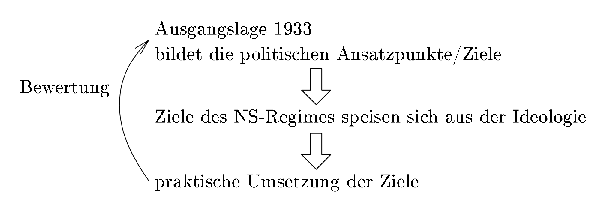
\includegraphics{bew-mass-ns.eps}
\caption{Bewertung der Wirksamkeit der Maßnahmen des NS-Regimes}
\label{pic:bew-mass-ns}
\end{figure}

Der Zustand der Weimarer Republik zu Anfang des Jahres 1933 bildete
die Ausgangslage für die Nationalsozialisten. Um deren Maßnahmen
hinsichtlich ihrer Wirksamkeit zu bewerten ist es zweckmäßig, zu
überprüfen, inwieweit sie Veränderungen gegenüber jener Ausgangslage
herbeiführten (siehe Abbildung \ref{pic:bew-mass-ns}) und wie die
Bevölkerung reagierte.

\begin{itemize}
\item wirtschaftliche Krise -- hohe Arbeitslosigkeit und Armut

\item Verhinderung wirtschaftlicher Erholung durch unfähige Demokraten
(\Nam{Brüning, Heinrich}{Brüning}s Deflationspolitik)

\item Wunsch nach
\begin{itemize}
\item Revision des \Ges{Vertrag von Versailles}{Vertrags von Versailles}

\item großdeutschem Reich -- Deutschland als militärische und
politische Großmacht

\item Verringerung der Arbeitslosigkeit
\end{itemize} 
\end{itemize}

%%%%%%%%%%%%%%%%%%%%%%%%%%%%%%%%%%%%%%%%%%%%%%%%%%%%%%%%%%%%%%%%%%%%%%

\subsection{Ziele der nationalsozialistischen Politik}

Aus dem vorhergehenden Abschnitt ergaben sich folgende Ansatzpunkte
für die Nationalsozialisten, um sich die Unterstützung der Bevölkerung
zu sichern:

\begin{itemize}
\item Wirtschaft
\begin{itemize}
\item Autarkie
\item Bekämpfung der Arbeitslosigkeit 
\end{itemize} 

\item Innenpolitik
\begin{itemize}
\item Ausschaltung der legalen Machtbasis
\item Zentralgewalt
\item Ausgrenzung der Nichtarier
\end{itemize}

\item Außenpolitik
\begin{itemize}
\item Revision des \Ges{Vertrag von Versailles}{Vertrags von Versailles}
\item Osterweiterung
\end{itemize}
\end{itemize}

Diese Ziele leiteten sich ebenfalls aus der Ideologie des
Nationalsozialismus ab, welche sich wiederum im \Ges{NSDAP,
Nationalsozialistische Deutsche Arbeiterpartei!Programm}{Programm der
NSDAP}\mycite{ProgNSDAP} niederschlug.

\endinput

\section{Innenpolitik}

\subsection*{NSDAP im Kabinett Hitler ab 30. Januar 1933}

\begin{description}
\item[\Nam{Hitler, Adolf}{Hitler}] Reichskanzler: Leitung der
Kabinettssitzungen, Bestimmung der politischen Richtlinien 

\item[\Nam{Frick, Wilhelm}{Frick}] Innenminister: verantwortlich für
die innere Sicherheit -- Vorbereitung und Durchführung von Gesetzen
und Notverordnungen (Zeitungs-, Versammlungs, Parteiverbot)

\item[\Nam{Göring, Hermann}{Göring}] Minister ohne Geschäftsbereich:
erhält das \ins{Reichskommissariat für das preußische
Innenministerium} -- Kontrolle über die preußische Polizei
\end{description}

%%%%%%%%%%%%%%%%%%%%%%%%%%%%%%%%%%%%%%%%%%%%%%%%%%%%%%%%%%%%%%%%%%%%%%

\subsection*[Maßnahmen Februar bis März 1933]{Maßnahmen Februar bis
März 1933\mycite[402]{gelbesGeschichts}}

Am \dat{1. Februar 1933} ließ \Nam{Hitler, Adolf}{Hitler} durch
\Nam{Hindenburg, Paul von}{Hindenburg} den \dat{Reichstag auflösen}.
Er begründete dieses Handeln damit, dass die Bildung einer
arbeitsfähigen Mehrheit im Parlament nicht möglich sei. Vorher hatte
er seine Scheinverhandlungen mit \Nam{Kaas, Ludwig}{Ludwig Kaas}
(Zentrum) scheitern lassen.

Danach begann der staatliche Terror, der die Ausschaltung
beziehungsweise Vernichtung der \jar{inneren} oder auch
\jar{Reichsfeinde} (Juden, gegnerische Politiker -- hauptsächlich KPD
und SPD) zum Ziele hatte. Gesetzliche Grundlage dafür war die
\dat{\ges{Reichstagsbrandverordnung} vom 28. Februar}. Diese führte
die \beg{Schutzhaft} ein; außerdem entstanden erste
Konzentrationslager.

Außerdem beeinflusste man im Hinblick auf die für \dat{März}
angesetzten \dat{Wahlen} die Bevölkerung durch Forcierung
propagandistischer Maßnahmen.

%%%%%%%%%%%%%%%%%%%%%%%%%%%%%%%%%%%%%%%%%%%%%%%%%%%%%%%%%%%%%%%%%%%%%%

\subsection*[Maßnahmen März 1933 bis August 1934]{Maßnahmen März 1933
bis August 1934\mycite[392\,--\,398]{gelbesGeschichts}}

Siehe dazu das Arbeitsblatt mit der Übersicht.

\endinput

\section{Wirtschaft}

\begin{aufgabe}
zu eingebunden -- siehe Hefter
\end{aufgabe}

\begin{itemize}
\item \jar{Rettung} der Bauern -- Ernährungs- und Lebensgrundlage
\item \jar{Rettung} der Arbeiter --
\textquote[{\mycite[139]{DeuzwDemuDikt}}]{umfassende[r] Angriff
gegen die Arbeitslosigkeit}
\item Autarkie $\Rightarrow$ Krieg
\end{itemize}

\begin{figure}
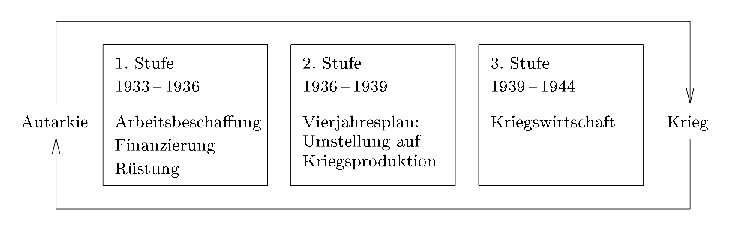
\includegraphics[width=\textwidth]{hit-stufpla.eps}
\caption{\Nam{Hitler, Adolf}{Hitler}s Stufenplan}
\label{pic:hit-stufpla}
\end{figure}

Diese Ziele wollte \Nam{Hitler, Adolf}{Hitler} mit seinem
\ges{Stufenplan} (siehe \ref{pic:hit-stufpla}) erreichen. Dessen erste
Stufe soll hier näher beleuchtet werden. \mar{Und die anderen?}

Die dargestellten Maßnahmen folgten der Politik des \emph{deficit
spending}\index{deficit spending}, welches durch den
Reichswirtschaftsminister und Reichsbankpräsidenten \Nam{Schacht,
Hjalmar}{Hjalmar Schacht} angeregt wurde. Er erfand auch das
sogenannte \emph{Mefo-Wechselsystem}\index{Mefo-Wechsel} zur
Finanzierung der Rüstungsaufträge. Nach diesem bezahlte nicht das
Deutsche Reich direkt selbst, sondern eine Scheinfirma, die \Ins{Mefo,
Metallurgische Forschungsgesellschaft}{Metallurgische
Forschungsgesellschaft} (Mefo) akzeptierte von der Industrie
ausgestellte Wechsel, die bis 1938 einzulösen waren. Die weiteren
Details sind hier unwichtig. Dieses System bot einige
Vorteile.\mar{Doch welche?}


\subsection{Erste Stufe: Wirtschafts- und
Sozialpolitik\mycite{LemoWirtsch}}
\mar{Wo sind die anderen?}

\subsubsection{wirtschaftliche Maßnahmen:}

\begin{itemize}
\item leichter Wirtschaftsaufschung 1933 durch die
Arbeitsbeschaffungsmaßnahmen der vorherigen Regierungen
\item Arbeitsbeschaffungsprogramme (Straßenbau: Autobahn, Bauwesen:
Wohnungsbau) steuerliche Anreize $\Rightarrow$ Senkung der
Arbeitslosigkeit
\item ab \dat{Juni 1935 Reichsarbeits- und Wehrdienst} $\Rightarrow$
Senkung der Arbeitslosigkeit
\item NS-Regime baut auf Privateigentum -- Interessenübereinstimmung
zwischen Großindustrie (Profitgier) und NS-Regime (forcierte
Kriegsvorbereitung)
\item schnelle Aufrüstung der modernen Industriezweige, beispielsweise
des Fahrzeugbaus
\item öffentliche Wirtschaftsforderung, vor allem durch
Rüstungsaufträge
\item Förderung der Landwirtschaft durch das
\dat{\ges{Reichserbhofgesetz} vom 29. September 1933}, das 
Hofteilung, Verkauf und Belastung mit Hypotheken verbot, dadurch aber
auch Neuinvestitionen stark behinderte.
\end{itemize}

\subsubsection{sozialpolitische Maßnahmen:}

\begin{itemize}
\item 1. Mai als staatlicher Feiertag bei voller Lohnfortzahlung
(1933 \ins{Feiertag der nationalen Arbeit}, ab 1934 \ins{Nationaler
Feiertag}) \index{1. Mai}
\item Gründung der Organisation \dat{\ins{Kraft durch Freude} im
November 1933} $\Rightarrow$ kulturelle und touristische
Freizeitbeschäftigungen für große Teile der Arbeiterschaft
\item Sofortmaßnahmen gegen Hunger, Armut und Verelendung, darunter
die Gründung des \dat{\Ins{Winterhilfswerk}{Winterhilfswerks}}
\end{itemize}

\endinput

\section{Außenpolitik}

Liest man \Nam{Hitler, Adolf}{Hitler}s Regierungserklärung vor dem
Reichstag vom 17. Mai 1933\mycite{HitlRegErklFrie} und seine Rede vor
der Reichswehrführung in Berlin vom 3. Februar des selben
Jahres\mycite{HitlRedRwfueh}, wird der zweischneidige Charakter seiner
Außenpolitik deutlich: Während er vor dem Reichstag von einer Heilung
der Wunden des Versailler Vertrages innerhalb der Grenzen der Verträge
und durch friedliche Auseinandersetzung mit \enquote{den Nationen}
spricht, fordert er vor der Reichswehr einen \enquote{Kampf gegen
Versailles} und \enquote{Sorge für die Bundesgenossen} unter
Verwendung kriegerischer Mittel.

Man erkennt also eine Verschleierungstaktik, die die eigentliche
Kriegsvorbereitung durch den scheinbaren Weg über Verträge verdecken
sollte. Zu den konkreten Maßnahmen siehe Tabelle
\ref{tab:massn-hitl-ausspol}. Für Karikaturen zu dem Thema siehe den
Hefter.

\begin{table}
\caption{Außenpolitische Maßnahmen Hitlers}
\label{tab:massn-hitl-ausspol}

\begin{tabularx}{\textwidth}{cXX}
\toprule
Jahr    & verschleiernd     & kriegsvorbereitend \\ 
\midrule
1933 & Konkordat mit dem Papst\index{Reichskonkordat} & \\
     & \multicolumn{2}{c}{Austritt aus dem
Völkerbund}\index{Völkerbund!Austritt des Deutschen Reiches}   \\

1934 & \ges{Deutsch-Polnischerr -Nichtangriffspakt} &  \\

1935 & Rückgliederung des Saarlands
(Volksabstimmung)\index{Saarland!Rückgliederung} &  \\
     & \ges{Flottenabkommen} mit Großbritannien &  \\

1936 & \Ins{Olympische Spiele!Deutschland}{Olympische Spiele} in
Deutschland & Rheinlandbesetzung \index{Rheinland!Besetzung} \\

1937 &  & Beitritt Italiens zum \ges{Antikominternpakt} -- \ins{Achse
Berlin\,--\,Rom\,--\,Tokio}\\

1938 &  & Anschluss Österreichs\index{Österreich!Anschluss an das
Deutsche Reich} \\

     &  & Sudetenkrise\index{Sudetenkrise} -- \ges{Münchener Abkommen} \\

1939 &  & \ges{Deutsch-Sowjetischer Nichtangriffspakt} mit geheimem
Zusatzprotokoll \index{Zusatzprotokoll} \\
\bottomrule
\end{tabularx}
\end{table}

\endinput

Hohohohohoho.

\section{Ausschaltung realer und vermeintlicher Gegner des NS-Regimes}
\label{sec:aussch-gegner}

\begin{aufgabe}
Erläutern Sie ideologische Grundlagen der Ausschaltung vermeintlicher
Gegner!

Beschreiben Sie die Umsetzung der Ideologie an den beiden
vermeintlichen Gegnergruppen! 

Bewerten sie die Maßnahmen auf der Basis demokratischer Politik- und
Moralvorstellungen!
\end{aufgabe}

\begin{aufgabe}
Arbeiten Sie aus dem Text die elemente des historischen Gesamtrahmen,
in dem sicher nationalsozialistische Massenmord entwickelten, heraus!

Der Autor behauptet, dass die Rolle Hitlers entscheindend für die
Judenverfolgung/-vernichtung war. Erarbeiten Sie die dazu gehörende
Argumentation anhand des Textes und die zu Grunde liegenden
ideologischen Ansätze!

\Nam{Friedländer, Saul}{Friedländer} nennt die ideologische
Radikalisierung des ausgehenden 19. Jahrhunderts als einen Faktor, der
in Kombination mit weiteren den Holocaust \enquote{vorbereitete}.
Überprüfen Sie diese Theorie der Radikalisierung innerhalb der
Maßnahmen des Regimes von 1933 bis 1945!
\end{aufgabe}


\begin{description}
\item[Grundlage:] Rassenideologie und Sozialdarwinismus
\index{Rassenideologie} \index{Sozialdarwinismus}
\item[Ziel:] Verhindern der Beeinträchtigung des \nat{deutschen
Volkskörpers} und Schaffung der \nat{reinen Rasse}
\end{description}

Die Höherentwicklung des deutschen Volkes (\nat{Herrenmensch}) wurde
laut Ideologie bedroht durch\footnote{Beide Bereiche greifen
ineinander. Die Trennung dient nur der Veranschaulichung.}\mar{Das ist
ein Fall von Scheinheiligkeit.}:

\begin{multicols}{2}
Unerwünschtes (\nat{lebensunwertes}) Leben:
\nat{schlechte Erbanlagen} bedrohen die Höherentwicklung des Volkes
sowie der Menschheit.

$\rightarrow$ \nat{Rassenhygiene}\\

\emph{Euthanasie}

\columnbreak

Juden und \nat{Art-}/\nat{Rassenfremde}: \nat{rassisch bedingte 
Verderbtheit der Juden als minderwertige Rasse}

$\rightarrow$ Rassenantisemitismus\\

\emph{\beg{Holocaust}}
\end{multicols}

%%%%%%%%%%%%%%%%%%%%%%%%%%%%%%%%%%%%%%%%%%%%%%%%%%%%%%%%%%%%%%%%%%%%%%

\subsection{Euthanasie}
\label{ssc:Euthanasie}
\index{Euthanasie}

\subsubsection{Gesetzliche Grundlagen}

\begin{chronik}
\item[14.\,7.\,1933] \ges{Gesetz zur Verhütung erbkranken Nachwuchses}:
Zwangssterilisierung von vermeintlich Erbranken -- circa 6\,000 Tote,
am meisten Frauen

\item[26.\,6.\,1935]
Ergänzung: Legalisierung des Schwangerschaftsabbruchs bei
diagnostizierter Erbkrankheit

\item[15.\,9.\,1935]
\ges{Gesetz zum Schutz des deutschen Blutes und der deutschen Ehre}:
siehe \ref{sss:nürnberger-ges}

\item[18.\,10.\,1935]
\ges{Ehegesundheitsgesetz}: Verbot von Eheschließungen mit geistig
Behinderten und Erbkranken

\item[1.\,9.\,1939]
\emph{Geheimer Führererlaß}: Ermächtigung zur Durchführung der
Euthanasie
\end{chronik}

\subsubsection{Aktion T4}
\index{Aktion T4}

\setlength{\parskip}{0mm}

Diese nach dem Krieg nach der Adresse -- Tiergartenstraße 4 -- der
Euthanasiezentrale in Berlin benannte Aktion beinhaltete die Umsetzung
des Euthanasiebefehls. Der daran beteiligte Personenkreis teilte
sich in vier Aufgabenbereiche:

Die \ins{Reichsarbeitsgemeinschaft Heil- und Pflegeanstalten} (Leiter:
\Nam{Heyde, Werner}{Werner Heyde} (medizinisch), \Nam{Bohne,
Gerhard}{Gerhard Bohne} (Verwaltung)) war für die Erfassung der Opfer
zuständig und verschickte zu diesem Zweck ab Ende 1939 Meldebögen, die
Auskunft über Art und Dauer der Krankheit und die Arbeitsfähigkeit
verlangten.

Die \ins{Gemeinnützige Stiftung für Anstaltspflege} (Leiter:
\Nam{Schneider, Willy}{Willy Schneider}) diente als offizieller
Arbeitgeber der etwa 400 T4-Mitarbeiter.

Die \ins{Zentralverrechnungsstelle Heil- und Pflegeanstalten} (Leiter:
\Nam{Kaufmann, Gustav a.}{Gustav A. Kaufmann}) wickelte die Kosten ab.

Die \ins{Gemeinnützige Krankentransport GmbH} (Leiter: \Nam{Vorberg,
Reinhold}{Reinhold Vorberg}) fuhr mit meist grauen Bussen die Opfer in
die Zwischen- beziehungsweise Tötungsanstalten.\\

\noindent Die Aktion T4 begann 1939 mit der Kindereuthanasie, dem
an mindestens 5\,000 erbkranken oder behinderte Kindern und
Säuglingen.  Wenig später wurden die Tötungen auf Erwachsene
ausgeweitet. Etwa 70\,000 geistig Behinderte, psychisch Kranke, mehr
als fünf Monate stationär Behandelte, Straftäter und
\nat{Fremdrassige} wurden dabei vergast.

Aufgrund von Protesten der Kirche, der Angehörigen und in der
Bevölkerung stellte man die Vergasungsaktionen 1941 offiziell ein. Da
man aber wegen des Luftkriegs gegen Deutschland immer mehr
Krankenhausplätze benötigte, begann nun die sogenannte \emph{Wilde
Euthanasie}\index{Wilde Euthanasie}: Etwa 30\,000 Menschen wurden
heimlich vergiftet oder zu Tode gehungert.

%%%%%%%%%%%%%%%%%%%%%%%%%%%%%%%%%%%%%%%%%%%%%%%%%%%%%%%%%%%%%%%%%%%%%%

\subsection{Die Verfolgung der Juden}
\label{ssc:juden-verf}
\index{Holocaust}
\index{Judenverfolgung}

% Breite der ersten Spalte
\newlength{\frstcoljud}
\settowidth{\frstcoljud}{Phase}
% Breite der übrigen Spalten
\newlength{\othcol}
\newlength{\othcolsum} % der ganze Rest
\setlength{\othcolsum}{\textwidth}
\addtolength{\othcolsum}{-\frstcoljud}
\setlength{\othcol}{0.25\othcolsum}
\addtolength{\othcol}{-2\tabcolsep}

\begin{tabular*}{\textwidth}{p{\frstcoljud}*{4}{p{\othcol}}}
Phase & \Rm{1} & \Rm{2} & \Rm{3} & \Rm{4} \\
      & 1933-35 & 1935-38 & 1938-41 & 1941-45 \\
      & Boykottaktio"-nen & Ausgrenzung durch Gesetz und Terror
      & Deportation & Endlösung
\end{tabular*}

\subsubsection{Boykottaktionen\mycite[135, 136]{GeschDrReich}}
\label{sss:boykott}
\index{Judenboykott}

\begin{chronik}
\item[1.\,--\,3.\,4.\,1933]
befristeter\footnote{Laut Frau Seipold schlug die Aktion fehl, da die
Bevölkerung aus Gewohnheit weiter bei Juden einkaufte.
\cite[135]{GeschDrReich} stellt das etwas anders beziehungsweise
differenzierter dar.} Boykott jüdischer Geschäfte\footnote{Diese
Aktion bildete das Ende der spontanen Gewalt gegen die jüdische
Bevölkerung. Was folgte, waren organisierte Verbrechen.}

\item[7.\,4.\,1933]
\ges{Gesetz zur Wiederherstellung des Berufsbeamtentums} (ein Art
staatlicher \emph{Arierparagraph}): Entlassung von
\nat{\beg{Nicht-Ariern}} aus dem öffentlichen Dienst

\item[7.\,4.\,1933]
Möglichkeit des Entzugs der Zulassung jüdischer Anwälte

\item[April 1933]
\ges{Gesetz gegen die Überfüllung der deutschen Schulen und
Hochschulen}: Verdrängung der Juden aus den
Bildungsanstalten\footnote{Der vollständige Ausschluß erfolgte 1938.}

\item[5.\,10.\,1933]
\ges{Schriftleitergesetz}: Verdrängung jüdischer Journalisten aus den
Redaktionen

\item[1934]
Pause von antijüdischen Gesetzen
\end{chronik}


\subsubsection[\dat{Nürnberger Gesetze 15. September 1935}]
{\dat{Nürnberger Gesetze 15. September 1935}
\mycite[417-419]{gelbesGeschichts}}
\label{sss:nürnberger-ges}
\index{Nürnberger Gesetze}

\paragraph{\ges{Reichsbürgergesetz}} 
Juden verloren alle politischen Bürgerrechte -- sie wurden statt
als \nat{Reichsbürger} nur noch als \nat{Staatsangehörige}
gesehen und somit aus der \emph{Volksgemeinschaft} ausgeschlossen.

\paragraph{\ges{Gesetz zum Schutz des deutschen Blutes und der
deutschen Ehre}}
Diese Gesetz verbot Juden

\begin{itemize}
\item Ehen und außereheliche Beziehungen mit \nat{Ariern}
\item die Beschäftigung \nat{arischer} Dienstmädchen unter 45
Jahren
\item das Hissen der \nat{Reichs- und Nationalflagge} und das
Zeigen der \nat{Reichsfarben}
\end{itemize}

In den Folgejahren wurden die Rechte der Juden durch Sondergesetze und
Verordnungen immer weiter eingeschränkt,
beispielsweise\footnote{In \cite[135-137]{GeschDrReich} ist dies
differenziert dargestellt.}:

\begin{itemize}
\item Entfernung aus Beamtenpositionen und Wegfall der Pensionen
\item Boykottierung jüdischer Geschäftsleute und Industrieller
\item Entzug jeglichen Rechtsschutzes
\item Ungültigmachung mit Juden geschlossener Verträge
\item Zutrittsverbot zu Hotels, Pensionen, kulturellen Einrichtungen
und Parks
\end{itemize}

\noindent $\Longrightarrow$ völlige Entrechtung und gesellschaftliche
Isolierung der Juden \\

Im Hinblick auf die \dat{Olympischen Spiele} in Deutschland reduzierte
man die Repressalien \dat{1936} wieder, nur um sie im folgenden Jahr
erneut zu forcieren.


\subsubsection{\dat{Reichspogromnacht 9./10. November 1938}}
\label{sss:pogromnacht}
\index{Reichspogromnacht}
\index{Reichskristallnacht}

Am \dat{7. November 1938} verübte \Nam{Grynspan, Herschel}{Herschel
Grynszpan} in Paris ein Attentat auf den dortigen Botschaftssekretär
\Nam{Rath, Ernst vom}{Ernst vom Rath}.  Dieses nahmen die
Nationalsozialisten in Deutschland zum Anlaß und Vorwand für
gewaltsame Aussshreitungen gegen Deutsche jüdischen Glaubens zwei Tage
später.

Im Zuge derer kam es zu Morden und Plünderungen, Synagogen, jüdische
Gebetshäuser, Friedhöfe, Geschäfte und Wohnungen wurden in Brand
gesteckt beziehungsweise zerstört. Der Name \emph{Reichskristallnacht}
rührt von den zahlreichen Fensterscheiben her, die in jener Nacht
zerschlagen wurden.

Die Folgen der \emph{Novemberpogrome} waren mindestens 1\,300 Tote,
mehr als 1\,400 zerstörte Synagogen, Verhaftungen und Deportationen
und weitere Verschlechterung der Lebensbedingungen für Juden. Für die
entstandenen Schäden von ungefähr 1,12 Milliarden Reichsmark mußten
die Opfer selbst aufkommen.

Mit dem endgültigen Verlust finanzieller Mittel wurde den Juden eine
eventuelle Ausreise aus noch weiter erschwert.


\subsubsection[Radikalisierung der Judenpolitik \dat{September
1939\,--\,1941}]
{Radikalisierung der Judenpolitik \dat{September
1939\,--\,1941}\mycite[209, 216]{GeschDrReich}\mycite[433,
434]{gelbesGeschichts}}
\label{sss:rad-jud-pol}

\paragraph{Deportationsmaßnahmen/-pläne} \index{Deportation}
Durch ihre Kriegserfolge angespornt, stellten die Nationalsozialisten
verschiedene Pläne, die Juden aus Europa zu verbannen, auf. Diese
wurde jedoch aufgrund der schieren Anzahl zu Deportierender nicht
umgesetzt: 

\begin{chronik}
\item[1939\,--\,1941]
Zwangsumsiedlung nach Polen, Zusammenfassung und Isolierung in
\beg{Ghettos} \index{Ghetto}

\item[1940]
(Sieg über Frankreich): \beg{Madagaskarplan} \index{Madagaskarplan}

\item[1941]
(Überfall auf die UdSSR): Umsiedlung nach Sibirien
\end{chronik}


\paragraph{Vorgehen der SS-Einsatztrup"-pen beim Überfall auf Polen}
während des Überfalls auf Polen führten die SS-Einsatztrup"-pen im
Schatten der Wehrmacht \nat{politische Säuberungen} durch: Mit dem
iel der Ausrottung der jüdischen Bevölkerung kam es zu
assenerschießungen und Massakern. In den ersten Kriegswochen starben
abei circa 5\,000 Menschen.

ußerdem wurde die Kennzeichnungspflicht für Juden eingeführt und
man pferchte sie in Ghettos zusammen, wo sie Zwangsarbeit für die
Rüstungsindustrie zu leisten hatten.

\paragraph{Vertreibung der Juden nach dem Polenfeldzug}
\index{Deportation}
Mit der Begründung, Wohnraum werde \nat{aus kriegswirtschaftlichen
Gründen dringend benötigt}, deportierte man die Juden in Lager
in der Gegend von Lublin und im \ort{Generalgouvernement}. Das geschah
zunächst Bewohnern des \ort{Gaus Warteland}, ein halbes Jahr später
denen aus \ort{Pommern}. Im \dat{Februar 1940} vertrieb man die
Juden aus der Gegend von \ort{Stettin} und im \dat{März 1940} aus
\ort{Schneidemühl} in Preußen.

\paragraph{Vorgehen gegen die jüdische Bevölkerung während des
Krieges gegen die Sowjetunion}
Mit dem Krieg gegen die UdSSR wurden die Tötungsaktionen des Überfalls
auf Polen fortgesetzt. Neben der Wehrmacht, die dabei in die
Machenschaften der SS integriert wurde, rekrutierte man nun auch Teile
der Bevölkerung als \nat{Reserve-Polizeibataillone} sowie verbündete
Truppen, vor allem aus Weißrußland und Rumänien.

Von den 4,7 Millionen sowjetischen Juden kamen so bis Ende 1942 2,2
Millionen zu Tode.


\subsubsection{Konzentrations- und Vernichtungslager -- Die
\nat{Endlösung der Judenfrage}}
\label{sss:konz-vern-endl}
\index{Konzentrationslager}
\index{Vernichtungslager}
\index{Endlösung}

\begin{chronik}
\item[Juni 1941]
Vergasungsanlagen für \ort{Auschwitz}, Einsatz ab Herbst als
Vernichtungslager\footnote{Nach \ort{Chełmno}, wo noch die sogenannten
\ort{Gaswagen} verwendet wurden\cite{WikChelmno}, war es damit das
zweite Vernichtungslager und sollte das größte derer werden.}

\item[31.\,7.\,1941] Anweisung an \Nam{Heydrich, Erwin}{Reinhard
Heydrich}, eine \nat{Endlösung der Judenfrage} zu finden

\item[20.\,1.\,1942]
\emph{Wannseekonferenz}:
\begin{itemize}
\item Organisation und Koordination der Deportation der europäischen
Juden
\item Beschluß, Juden in ganz Europa als Arbeistkräfte auszubeuten und
zu ermorden\footnote{Laut \cite{WikWannsee} war dieser Beschluß
faktisch schon gefaßt. Ich füge ihn hier ein, da sich kein anderer
Platz ergeben hat.}
\end{itemize}

\item[1942]
Errichtung weiterer Vernichtungslager in \ort{Bełżec}, \ort{Sobibór},
\ort{Treblinka} und \ort{Majdanek}
\end{chronik}

\endinput

\section[Widerstand]{Widerstand\mycite[116-125, 230-245]{GeschDrReich}}
\label{sec:widerstand}
\index{Widerstand gegen den Nationalsozialismus}

\begin{aufgabe}
Begründen Sie, warum trotz der Radikalität und Unmenschlichkeit des
Regimes der innerdeutsche Widerstand realtiv begrenzt blieb! 
\end{aufgabe}

\subsection[Definition]{Definition\mycite{WidDefschwieBeg}}

Es gibt immer wieder Debatten, wie der Begriff des Widerstands im
Nationalsozialismus zu definieren sei.\footnote{Selbst das hier
verwendete \cite{WidDefschwieBeg} weist hier Fehler in der logischen
Durchführung auf.} So schlug \Nam{Broszat, Martin}{Martin Broszat} in
den frühen Achtzigerjahren vor: \enquote{Wirksame Abwehr, Begrenzung,
Eindämmung der NS-Herrschaft oder ihres Anspruchs, gleichgültig von
welchen Motiven, Gründen und Kräften her.}

Es gab jedoch zahlreiche Kritik, die entgegesetzte, dass jene
Definition den Begriff zu weit fasse und schon bei \emph{Haltungen}
beginne, während man erst bei \emph{Handlungen} einsetzen
dürfe.\footnote{Ich bin anderer Ansicht. \enquote{Wirksame Abwehr,
Begrenzung, Eindämmung} sind für mich keine bloßen Haltungen.}
Weiterhin greift man die fehlende Berücksichtigung der Motive an.

Die Tendenz geht als hin zum Widerstand als
\textquote[\mycite{WidDefschwieBeg}]{Handeln, das auf grundsätzlicher
Ablehnung des Nationalsozialismus beruhte, das aus ethischen,
politischen, religiösen, soialen oder individuellen Motiven darauf
abzielte, zum Ende des Regimes beizutragen}.

Tabelle \ref{tab:widerst-def} gibt einen Überblick über verschiedene
Möglichkeiten der Definition.

% verfluchter Blocksatz
\begin{table}
\caption{Definitionen für \emph{Widerstand}\mycite{WidDefschwieBeg}}
\label{tab:widerst-def}

% Berechnung der Spaltenbreiten
\newlength{\colwidth}
\setlength{\colwidth}{0.33\textwidth}
\addtolength{\colwidth}{-2\tabcolsep}

\renewcommand*{\arraystretch}{1.5}

\begin{tabular*}{\textwidth}{*{3}{p{\colwidth}}}
\toprule

\multirow{2}{\colwidth}{\centering Widerstand im weitesten Sinn} &
\multicolumn{2}{c}{Widerstand im engeren Sinn} \\

\cmidrule{2-3}

&
kritische bis abweisende Haltung der Verweigerung und Selbstbehauptung
&
bewusste Anstrengung zur Änderung der Verhältnisse \\

\midrule

zusammenfassender Oberbegriff für gegen den Nationalsozialismus als
Ideologie und praktizierte Herrschaft gerichtete verschiedenartige
Einstellungen, Haltungen und Handlungen &
\emph{Verweigerung} als persönliche Abwehr von Herrschaftsanspruch und
Selbstbehauptung von Gruppen &
bewusster persönlicher Einsatz, verbunden mit einhergehenden
Gefährdungen \\

Umfasst also auch beispielsweise ins Exil geflohene, die kaum
Möglichkeit zur Einwirkung auf das nationalsozialistische Regime
hatten und die die sich weder durch Lockungen noch durch Zwang vom
Nationalsozialismus vereinnahmen ließen. &
\emph{Opposition} als Haltung grundsätzlicher Gegnerschaft gegen das
Unrechtsregime -- passiver Widerstand &
beispielsweise Planung des Sturzes der Diktatur (Attentate)
einhergehend mit der Errichtung einer neuen Gesellschaftsordnung --
aktiver Widerstand \\

\bottomrule 
\end{tabular*}
\end{table}

%%%%%%%%%%%%%%%%%%%%%%%%%%%%%%%%%%%%%%%%%%%%%%%%%%%%%%%%%%%%%%%%%%%%%%

\subsection{Gruppen}

Die deutschen Widerstandsgruppen kamen aus verschiedenen
gesellschaftlichen Schichten. Dabei ist der Mittelstand kaum
ernennenswert; dessen größte Teile waren dem \index{Hitler-Mythos}
Hitler-Mythos erlegen.

Etwas mehr, aber dennoch nur wenig, tat sich bei den Vertretern der
Industrie: Hier waren es hauptsächlich \Nam{Bosch, Robert}{Bosch} und
\Nam{Krupp von Bohlen und Halbach, Gustav}{Krupp}, die \Nam{Goerdeler,
Carl Friedrich}{Goerdeler} unterstützten und andere, die Kontakte zum
amerikanischen Geheimdienst unterhielten. Inwiefern man dabei jeweils
von \emph{Widerstand} sprechen kann, ist natürlich fragliche.

Schließlich formierten sich im politischen Lager zahlreiche locker
zusammengeschlossene Gruppen, die aber meist nur das gemeinsame Ziel
der Beseitigung des Regimes verband.

Alle waren allerdings der Meinung, dass die Befreiung vom
Nationalsozialismus von Deutschland selbst aus erfolgen müsse, da nur
so eine \emph{bedingungslose Kapitulation}, wie sie die Alliierten
forderten abgewendet und Souveränität und Verhandlungsfähigkeit
Deutschlands erhalten werden könnten.\mycite[191-193]{DeuzwDemuDikt}

Dabei waren die Widerstandsbewegungen im Ausland, beispielsweise die
\ins{R\'e{}sistance} in Frankreich und \index{Partisanen}
\ins{Partisanengruppen} in Polen, der Sowjetunion, Jugoslawien,
Griechenland und Italien, zum Teil viel reger und erfolgreicher als im
Reich selbst. Das lag daran, dass sich die politischen und geistigen
Strömung unter dem Eindruck eines gemeinsamen Besatzers zu einem
nationalen Befreiungskampf einten, während die Widerstandsgruppen in
Deutschland nur wenig zusammenarbeiteten, während die
Widerstandsgruppen in Deutschland nur wenig zusammenarbeiteten.

Anfangserfolge im Krieg hatten den \index{Hitler-Mythos} Hitler-Mythos
befeuert, Beamte und andere hatten einen Eid auf \Nam{Hitler,
Adolf}{Hitler} geschworen. Der Terror durch die \ins{Gestapo} und
scharfe Gesetze, die Kritik am Regime und Kontakte zum Ausland und zu
Ausländern im Inland verboten, taten ihr Übriges, um eine
Ablehnungshaltung der Bevölkerung gegenüber Widerständlern und
gewaltsamer Beseitigung der Obrigkeit zu schaffen.

Allerdings kehrte sich diese Haltung mit fortschreitendem
Kriegsverlauf immer weiter ins Gegenteil. Die Verschlechterung des
Zustands, insbesondere der Versorgungslage, ließ den Wunsch nach
baldigem Kriegsende immer größer werden; die unerwartete Kriegslage
verunsicherte das Regime, die Herrschaftsstruktur wurde löchrige,
sodass die Bevölkerung allmählich das Vertrauen verlor.

Im Folgenden sollen beispielhaft einige Gruppen mit ihren Motiven,
Zielen und Handlungen aufgeführt werden, die sich auch schon vor den
meisten Anderen gegen die nationalsozialistische Herrschaft gerichtet
hatte. Dabei werden sämtliche Grade von Kritik bis zum aktiven
Widerstand berücksichtigt.


\subsubsection[Kommunisten und Sozialdemokraten]{Kommunisten und
Sozialdemokraten\footnote{Die beiden Gruppen wirkten keineswegs von
Anfang an gemeinsam im Widerstand und auch später gab es teilweise
große Differenzen. So kämpften die Kommunisten zunächst ebenso gegen
die Sozialdemokraten und auch die Wahl der Mittel fiel unterschiedlich
aus: Während die Ersteren einigermaßen radikal und ohne Rücksicht auf
Verluste vorgingen, während die Anderen mehr Vorsicht walten ließen.}}
\index{Kommunismus}
\index{Sozialdemokratie}

Für deren Aktivitäten lagen natürlich ideologische Gründe vor.

\noindent Mittel:

\begin{itemize}
\item Flugblätter und Broschüren in großer Anzahl
\item Wandparolen
\item Demonstrationen
\item Fahnenhissen
\item Sprechchöre
\item Überzeugungsarbeit \enquote{von Mann zu Mann}
\item stille Verweigerung und
\textquote[{\mycite[120]{GeschDrReich}}]{öffentliche[s] Beharren auf
demokratischen und rechtsstaatlichen Idealen}
\item Milieubildung mit Nachbarschaftshilfe, Austausch von Meinungen,
Nachrichten und Spende von Trost
\item Fluchthilfe
\item Abhören ausländischer Sender
\item Zeitschriften und Publikationen, auch für das Ausland
\end{itemize}


\subsubsection{Kirchen}
\index{Widerstand!Kirchen}

Auch die Kirchen waren untereinander in ihrer Haltung gegenüber dem
Nationalsozialismus gespalten. Während die Katholiken sich zunächst
von \Nam{Hitler, Adolf}{Hitler} betören und täuschen ließen und später
eher seichte Mahnungen an das Regime richteten, wurde das anfängliche
Verlangen der Protestanten nach einem \nat{starken Mann} an der Spitze
des Staates befriedigt.

Allerdings vollzog sich mit der Zeit eine zunehmende Spaltung der
evangelischen Kirche in \Ins{Deutsche Christen}{Deutschen Christen}
als Anhänger des Nationalsozialismus und die \ins{Bekennende Kirche},
die ein entschlosseneres Unternehmen als die Katholiken an den Tag
legte.

Trotzdem muss man erkennen, dass weniger die Kirchen als Institutionen
selbst Widerstand leisteten, sondern eher christliche Einzelpersonen
-- besonders prominent sicherlich \Nam{Niemöller, Martin}{Martin
Niemöller} und \Nam{Bonhoeffer, Dietrich}{Dietrich Bonhoeffer} --
offen gegen den Nationalsozialismus vorgingen.\\

\noindent Kritikpunkte:

\begin{sloppypar}
\begin{itemize}
\item Kampf gegen Ordensgemeinschaften
(\nat{Klostersturm}\index{Klostersturm})
\item \textquote[{\mycite[121]{GeschDrReich}}]{\enquote{Pfaffenprozesse}
\index{Pfaffenprozesse} gegen Ordensgeistliche wegen angeblicher
Devisenschiebereien und Sittlichkeitsvergehen}
\item Eingriff des Staats in Kirchenangelegenheiten
\item Missachtung des \Ges{Reichskonkordat}{Reichskonkordats}
\item Rassenpolitik, Antisemitismus
\item Euthanasie
\item \nat{rassisch-völkische Weltanschauung}
\item Konzentrationslager
\item Willkür der \ins{Gestapo}
\item Missachtung christlicher Grundsätze
\end{itemize}
\end{sloppypar}

\noindent Mittel:

\begin{itemize}
\item Enzyklika \index{Enzyklika} \ges{Mit brennender Sorge}, geheim
vervielfältigt und verteilt
\item Eingaben\footnote{Diese waren eher zurückhaltender Art und
natürlich auch kaum erfolgreich.}
\item Reden von der Kanzel aus -- Predigten
\item \ins{Pfarrernotbund}
\item Untergrundarbeit
\end{itemize}


\subsubsection{Kreis um \Nam{Goerdeler, Carl Friedrich}{Carl Goerdeler}}

Hierzu gehörten hochrangige Militärs (beispielsweise \Nam{Beck,
Ludwig}{Generaloberst Ludwig Beck}), Wirtschaftsverantwortliche,
Industrielle, Gewerkschafter und andere vornehmlich konservative,
christliche und nationalliberale Bürger und Politiker. \\

\noindent Kritikpunkte:

\begin{itemize}
\item waghalsige Kredit-, Finanz- und Wirtschaftspolitik
\item Antisemitismus (negative Wirkung auf das Ansehen Deutschlands im
Ausland)
\item Entfernung des Denkmals für \Nam{Mendelssohn-Bartholdy,
Felix}{Felix Mendelssohn-Bartholdy} in Leipzig
\item Unterschätzung des Auslands
\item Kriegsbestrebungen
\end{itemize}

\noindent Ziele:

\begin{itemize}
\item Staatsstreich
\item Staats- und Gesellschaftsordnung auf Grundlage von
Rechtsstaatlichkeit, Moral, bürgerlichem Anstand und christlicher
Weltanschauung -- stark restaurativer Charakter
\item Kriegsende
\end{itemize}

\noindent Mittel:

\begin{itemize}
\item Kritik in Wirtschaftsgutachten für die Regierung
\item Werbung für Opposition gegen die Nationalsozialisten im Ausland
\item Knüpfung von Beziehungen zu Personen in verschiedensten
gesellschaftlichen Positionen
\item Einsatz des Militärs -- Verhandlungen mit hochrangigen
Offizieren
\end{itemize}


\subsubsection{Kreisauer Kreis\index{Kreisauer Kreis}}

Hier handelte es ich um eine Gruppe von Regimegegner
unterschiedlichster Profession, die sich auf dem Gut des \Nam{Moltke,
Helmuth James Graf von}{Helmuth James Graf von Moltke} in
\ort{Kreisau}, \ort{Niederschlesien}, zu Gesprächen traf. Führender
Kopf war neben dem Gutsbesitzer \Nam{Wartenburg, Peter Graf Yorck
von}{Peter Graf Yorck von Wartenburg}.

Bei dieser Gruppe muss man außerdem hervorheben, dass sie
hauptsächlich von den Verbrechen der Nationalsozialisten gegen Juden,
Kriegsgefangene und Bewohner der besetzten Gebiete zum Widerstand
angeregt wurden. Das war bei den bisher genannten Personen und
Körperschaften nicht primär der Fall.\\

\noindent Ziele\footnote{In diesem Abschnitt werden zahlreiche
Wortkombinationen verwendet, wie sie genau so in
\cite[236-238]{GeschDrReich} zu finden sind. Ich verzichte auf
ständige Anführungszeichen und Partikulärnachweise.}:

\begin{itemize}
\item Überwindung des Nationalsozialismus, des Machtstaats und des
Rassendenkens

\item Neuordnung und Neuorientierung von Staat und Gesellschaft
\begin{itemize}
\item Wiederherstellung eines humanen Rechtsstaats
\item Garantie von Glaubens- und Gewissensfreiheit
\item Recht auf Arbeit und Eigentum
\item Selbstbestimmung und Verantwortlichkeit statt Befehl und
Gehorsam
\item politische Verantwortung und Mitwirkung jedes Einzelnen statt
Diktatur und Unterwerfung
\item Gründung einer Völkergemeinschaft im Geiste internationaler
Toleranz
\end{itemize}

\item Bestrafung der nationalsozialistischen Verbrecher
\end{itemize}

\noindent Prinzipien:

\begin{itemize}
\item Humanität
\item christliche Ethik
\item Gerechtigkeit
\item Ablehnung von Gewalt\footnote{Hiermit ist hauptsächlich die
Ablehung eines gewaltsamen Sturzes des Regimes und einer Ermordung
\Nam{Hitler, Adolf}{Hitlers} gemeint. \Nam{Moltke, Helmuth James Graf
von}{Moltke} befürchtete nämlich, dass ein solches Vorgehen nach dem
Umsturz ähnlich der \emph{Dolchstoßlegende}\index{Dolchstoßlegende}
propagandistisch ausgeschlachtet würde.}
\end{itemize}


\subsubsection{Weitere}

Mit den genannten Gruppen ist ein großer Teil des Spektrums der Motive
und Ziele von Widerstandsgruppen abgedeckt. Für weitere Informationen,
insbesondere über die Attentate auf \Nam{Hitler, Adolf}{Hitler} und
über studentischen Widerstand wie den der \Ins{Weiße Rose}{Weißen
Rose} siehe auch \cite[239-245]{GeschDrReich}.

\endinput


\endinput

\part{Demokratie und Diktatur -- Anspruch und Wirklichkeit von
Gesellschaftsmodellen in der zweiten Hälfte des 20. Jahrhunderts}
\label{prt:dem-dikt2}
\thispagestyle{empty}

\chapter{Neubeginn im besiegten Land}
\label{sec:neubeginn}

\begin{chronik}
\item[8.\,5.\,1945]
bedingugslose Kapitulation Deutschlands -- offizielles Ende des
\emph{Zweiten Weltkriegs} \index{Zweiter Weltkrieg!Ende}

\item[5.\,6.\,1945]
\ges{Berliner Erklärung} \index{Berliner Erklärung} (USA,
Großbritannien, Frankreich, UdSSR): Übernahme der Regierungsgewalt und
des Oberkommandos der Wehrmacht durch die Alliierten

\item[17.\,7.\,--\,2.\,8.\,1945]
\ort{Postdamer} Konferenz \index{Potsdamer Konferenz}
\begin{itemize}
\item Aufteilung Deutschlands in vier Besatzungszonen
\index{Besatzungszonen}
\item Betrachtung der deutschen Wirtschaft als Einheit
\item Ziele: Dezentralisierung, Demokratisierung, Entmilitarisierung,
Entnazifizierung \index{Demokratisierung} \index{Dezentralisierung}
\index{Entnazifizierung} \index{Entmilitarisierung}
\item beinahes Scheitern der Verhandlungen über den Fragen der
Reparationen und der Ostgrenze
\end{itemize}
\end{chronik}

\section[Gründung der BRD]{Die Gründung der BRD\footnote{Es
handelt sich hier nur um einen groben Überblick. \label{ftn:grob-ueb}}
\mycite[333, 334]{WeltgeschNeuz}}
\label{sec:gruend-brd}
\index{BRD!Gründung}

\begin{chronik}
\item[Juli 1948]
Überreichung der \ges{Frankfurter Dokumente} an die
Ministerpräsidenten der Länder: Angebot zur Errichtung eines
westdeutschen Bundesstaates, Grundsätze für dessen Verfassung

\item[August 1948]
Erarbeitung eines Verfassungsentwurfes durch eine
Sachverständigenkommission als Beratungsgrundlage für den
\textsc{\Ins{Parlamentarischer Rat}{Parlamentarischen Rat}}

\item[8.\,5.\,1949]
Verabschiedung des Grundgesetzes durch den parlamentarischen Rat

\item[12.\,--\,23.\,5.\,1949]
Zustimmung der Westalliierten und der Bundesländer\footnote{Bayern
ratifizierte das Grundgesetz nicht, erkannte aber dessen
Rechtsverbindlichkeit an.} zum Grundgesetz 

\item[23.\,5.\,1949]
Inkrafttreten des \Ges{Grundgesetz für die Bundesrepublik
Deutschland}{Grundgesetzes für die Bundesrepublik Deutschland}

\item[14.\,8.\,1949]
freie, geheime, gleiche, direkte und allgemeine Wahl des ersten
\Ins{Deutscher Bundestag}{Deutschen Bundestages} durch die
westdeutsche Bevölkerung
\end{chronik}

\section[Gründung der DDR]{Die Gründung der DDR
\footref{ftn:grob-ueb}
\mycite[334, 335]{WeltgeschNeuz}}
\label{sec:gruend-ddr}
\index{DDR!Gründung}

\begin{chronik}
\item[10.\,7.\,1945]
zentrale Zulassung von Parteien in der \textsf{\ort{SBZ}} durch die
\beg{SMAD}

\item[14.\,7.\,1945]
Gründung des \Ins{Block antifaschistisch-demokratischer
Parteien}{Blocks antifaschistisch-demokratischer Parteien} --
Zusammenarbeit von KPD, SPD, CDU und LDPD
\begin{itemize}
\item nur einstimmige Beschlussfassung
\item Bindung für alle Parteien an die Beschlüsse
\item Festlegung eines nicht näher definierten gemeinsamen Weges
\end{itemize}

\item[22.\,4.\,1946]
Auf Druck der sowjetischen Gesatzungsmacht vereinigen sich SPD und KPD
zur SED\index{SED!Gründung}, da man befürchtete, dass die KPD in
freien Wahlen nicht genügend Stimmen gewinne.

\item[Feb. 1946]
Gründung des \textsf{\ins{FDGB}}\index{FDGB!Gründung}
(Einheitsorganisation) -- Während zwar
alle Parteien in der Leitung vertreten waren, sicherten sich die
Kommunisten dennoch die Vorherrschaft.

\item[Mitte März 1948]
Zusammentreten des \Ins{Zweiter Deutscher Volkskongresses}{Zweiten
Deutschen Volkskongresses} bestehend aus 2\,000
Delegierten\footnote{Die Stimmenmehrheit lag bei der SED und deren
Verbündeten} der Blockparteien und der Massenorganisationen
(beispielsweise FDJ und FDGB) auf Initiative der SED, Wahl des
\Ins{Deutscher Volksrat}{Deutschen Volksrates} (400 Mitglieder) --
Aufgabe: Ausarbeitung einer Verfassung für eine \enquote{unteilbare
deutsche Republik}

\item[19.\,3.\,1949]
Verabschiedung eines Verfassungsentwurfes durch den Deutschen Volksrat

\item[15./16.\,5.\,1949]
Wahl des \Ins{Dritter Deutscher Volkskongress}{Dritten Deutschen
Volkskongresses} durch die Bevölkerung der \ort{SBZ} nach
Einheitsliste.

Der \Ins{Dritter Deutscher Volkskongress}{Dritte Deutsche
Volkskongress} wählt den \Ins{Zweiter Deutscher Volksrat}{Zweiten
Deutschen Volksrat}, welcher sich zur provisorischen \ins{Volkskammer}
erklärt und die \ges{Verfassung der Deutschen Demokratischen Republik}
nach Bestätigung durch den \emph{Volkskongress} in Kraft setzt. Der
Präsident der DDR wurde \nam{Wilhelm Pieck}.

\item[7.\,10.\,1949]
Inkraftsetzung der \ges{Verfassung der Deutschen Demokratischen
Republik}

\item[15.\,10.\,1950]
Wahlen zur \ins{Volkskammer} über Einheitsliste\footnote{Artikel 51
der \ges{Verfassung der Deutschen Demokratischen Republik} sah
eigentlich eine Verhältniswahl vor.} durch die ostdeutsche
Bevölkerung
\end{chronik}

\endinput



\chapter{Das Demokratieverständnis in beiden deutschen Staaten}
\label{chp:demverst-beid-staat}
\index{Demokratieverständnis}

\section{Der Demokratiebegriff}
\label{sec:dem-begr}
\index{Demokratie}

\begin{aufgabe}
Untersuchen Sie, inwieweit die Verfassungen der neugegründeten Staaten
dem modernen Demokratiebegriff genügen!
\end{aufgabe}

\subsection*{Einteilung}

\begin{multicols}{2}
\noindent \emph{direkte Demokratie}:
direkte Entscheidungsfindung durch das Volk, beispielsweise in
Volksabstimmungen

\columnbreak

\noindent \emph{repräsentative (indirekte) Demokratie}:
Bürger wählen Repräsentanten, Sachentscheidungen durch Volksvertreter
\end{multicols}

\subsection*{Merkmale}

\begin{itemize}
\item Volkssouveränität (direkt, indirekt oder Mischform),
beispielsweise durch Wahlen oder Bürgerentscheide
\item Gewaltenteilung
\item Kontrolle der Exekutive und Legislative durch neutrale und
politisch unabhängige Judikative
\item Garantie der Menschen- und Bürgerrechte sowie der individuellen
Grundrechte (Schutz von Leben, Freiheit von Eigentum, Recht auf freie
Meinungsäußerung, Versammlungsfreiheit, Pressefreiheit)
\item Meinungspluralismus -- Parteienvielfalt
\item Verfassung
\end{itemize}

\endinput

\section[Volksaufstand in der DDR]{Volksaufstand in der
DDR\mycite{Dtl50erJ}}
\index{Voksaufstand}
\index{17. Juni 1953}

\subsection*{Ursachen}

\begin{itemize}
\item Militärblock- und Rüstungspolitik

\item Gründung der \Ins{Stasi, Ministerium für
Staatssicherheit}{Stasi} 1950 

\item wirtschaftliche Probleme:
\begin{itemize}
\item Planwirtschaft führt zu Priorisierung der Schwerindustrie und zu
Mangel in der Lebensmittel- und Konsumgüterproduktion
\item Rohstoffknappheit zwingt zu Importen
\item Reparationen
\item Ablehnung der Verstaatlichungsmaßnahmen (kaum noch
Privatwirtschaft), besonders in der Landwirtschaft führt zur
Auswanderung von Bauern und so zur weiteren
Verschärfung der Probleme.
\item Erhöhung der Arbeitsnorm
\end{itemize}

\item Unklarheit über die zukünftige Politik nach \Nam{Stalin,
Josef}{Stalin}s Tod am 5. Juni 1953

\item Erzwingung eines \jar{Neuen Kurses} durch die Sowjetunion am 9.
Juni:
\begin{itemize}
\item politische Lockerungen
\item Zugeständnisse an die Bauern und den Mittelstand
\item keine Rücknahme der Normerhöhung
\end{itemize}
\end{itemize}

%%%%%%%%%%%%%%%%%%%%%%%%%%%%%%%%%%%%%%%%%%%%%%%%%%%%%%%%%%%%%%%%%%%%%%

\subsection*{Forderungen}

Arbeiter waren die Initiatoren und Hauptträger des Aufstandes.
Deswegen war auch die Forderung nach der Rücknahme der Normerhöhung
tonangebend. Im Verlaufe der Proteste wurden aber auch politische
Probleme angeschnitten: Rücktritt der Regierung, Wiedervereinigung
Deutschlands, freie Wahlen, freie Parteien und Gewerkschaften.

%%%%%%%%%%%%%%%%%%%%%%%%%%%%%%%%%%%%%%%%%%%%%%%%%%%%%%%%%%%%%%%%%%%%%%

\subsection*{Verlauf}

Der Aufstand \dat{begann} bereits am \dat{16. Juni 1953} mit
Arbeitsniederlegungen an zwei berliner Großbaustellen
(\ort{Stalinallee}). Die Beteiligten zogen vor das Politbüro, wo
Industrieminister \Nam{Selbmann, Friedrich}{Selbmann} zu
beschwichtigen versuchte und die Normerhöhung zurücknahm. Dies war
jedoch vergeblich und die Protestierenden riefen über Boten und
Rundfunk auch die übrige Bevölkerung zum Streik auf.

So kam es am \dat{17. Juni} zu \dat{flächendeckendem Aufbegehren} in
cat 560 Städten der DDR -- hauptsächlich Industriestandorte wie
\ort{Leuna}, \ort{Wolfen} und \ort{Jena}. Die Demonstranten befreiten
Häftlinge aus den Gefängnissen, es kam zu Zusammenstößen mit der
Polizei. Darauf verhängte die \Ins{SMAD, Sowjetische
Militäradministration}{SMAD} am Mittag in den großen Städten den
Ausnahmezustand. Mithilfe sowjetischer Panzer wurde der Aufstand
blutig niedergeschlagen.

%%%%%%%%%%%%%%%%%%%%%%%%%%%%%%%%%%%%%%%%%%%%%%%%%%%%%%%%%%%%%%%%%%%%%%

\subsection*{Folgen}

\begin{itemize}
\item ca. 21 Tote, zahlreiche Verletzte 
\item Verfolgung und Inhaftierung der \jar{Rädelsführer} und andere
Beteiligter -- ca. 1400 Verurteilungen zu langjährigen
Zuchthausstrafen
\item \jar{Reinigung} der SED von \jar{feindlichen Elementen}
\item Festigung der Machposition \Nam{Ulbricht, Walter}{Walter
Ulbricht}s
\item anhaltende Furcht der Staatsführung vor einer Wiederholung des
17. Juni
\item Preissenkungen der \Ins{HO, Handelsorganisation}{HO}
\item Massenfluchtbewegung in den Westen $\Rightarrow$ Mauerbau (siehe
\ref{sec:mauerbau})
\item Ende der Reparationsentnahmen aus der laufenden Produktion durch
die UdSSR 1954
\end{itemize}

%%%%%%%%%%%%%%%%%%%%%%%%%%%%%%%%%%%%%%%%%%%%%%%%%%%%%%%%%%%%%%%%%%%%%%

\subsection*{Bewertung anhand des modernen Demokratiebegriffs}

\begin{itemize}
\item weitere Freiheitseinschränkungen
\item Beschluss der Niederschlagung allein durch die Exekutive
\item brutale Unterdrückung der Volkssouveränität
\end{itemize}

$\Longrightarrow$ keine rechtsstaatliche Lösung 

\endinput

\section[Bau der Berliner Mauer]{Bau der Berliner
Mauer\mycite{Dtl50erJ}}
\index{Mauerbau}
\index{Berliner Mauer}
\label{sec:mauerbau}

\subsection*{Ausgangssituation}

\dat{Seit 1945 strömten DDR-Bürger} in die BRD. Sie sahen darin einen
Ausweg aus den widrigen Verhältnissen des sozialistischen Staates:
Unzureichender Versorgung, fehlendem Fortschritt und
Zwangskollektivierung sowie totalitaristischem Anspruch der SED bei
äußerst geringem politischem Mitbestimmungsrecht in der DDR standen
wirtschaftlicher Aufschwung und ein hohes Maß an politischer Freiheit
in der BRD gegenüber.

So kam es, dass bis zum folgenden Mauerbau 2,7 Millionen Menschen,
darunter zahlreiche junge und hochqualifizierte Facharbeiter Richtung
Westen zogen. Diese fehlten der DDR beim Aufbau einer leistungsfähigen
Wirtschaft, weshalb \dat{schon 1946 die Grenzen} durch Zäune und
Alarmvorrichtungen \dat{gesichert} wurden. Die Grenze in Berlin war
jedoch weiterhin offen, sodass \dat{1959/60} der DDR der
wirtschaftliche Zusammbruch drohte.\mar{Chruschtschows
Berlin-Ultimatum auch?}

\subsection*{Verfaul}

Am \dat{12. August 1961} unterschreibt \Nam{Ulbricht, Walter}{Walter
Ulbricht} auf geheimen Beschluss und nach Erlaubnis der UdSSR den
Befehl, auch die berliner Grenze zu schließen. Daraufhin rückten in
der Nacht Abteilungen der \Ins{NVA, Nationale Volksarmee}{NVA}, der
\ins{Volkspolizei} und Kampfgruppen aus, riegelten die Sektorengrenzen
ab und sperrten die Verkehrswege. Innerhalb eines Jahres wurde dann
die eigentliche die Westsektoren umschließende Grenzbefestigungsanlage
bestehend aus Mauer, Zäunen, Wachtürmen, Hundelaufstreifen,
Selbstschussanlagen und anderen Sicherungseinrichtungen errichtet.

\subsection*{Folgen}

\begin{itemize}
\item ca. 899 Todesopfer bei Fluchtversuchen aus der DDR
\item Ausreise in den Westen nur noch bei Genehmigung
möglich\mar{Nicht vorher schon?}
\item Ende der Massenflucht
\item weitere Verschlechterung des Verhältnisses zwischen Bevölkerung
und Staat
\item Auseinanderreißung von Familien
\item Verlust von ca. 60\,000 Arbeitsplätzen (Pendler)
\item Verschlechterung der Infrastruktur durch zerschnittenes
Verkehrsnetz
\end{itemize}

\subsection*{Bewertung anhand des modernen Demokratiebegriffs}

In Bezug auf die Verletzung der Grund- und Menschenrechte (siehe
Grundgesetz) stehen sich hier verschiedene Meinungen gegenüber:
Einerseits bedeutete der Mauerbau weitreichende Einschränkung der
Freizügigkeit und persönlichen Freiheit. Andererseits sah
\Nam{Kennedy, John Fitzgerald}{Kennedy} darin die bessere Alternative
gegenüber Krieg\mycite{WikMauer} und der britische Premierminister
\Nam{Macmillan, Maurice Harold}{Harold Macmillan} meinte, dass der
Stopp des Auswanderungsstroms
\textquote[\mycite{MacmillanMauer}]{nothing illegal} sei.

Ungeachtet dessen umging die DDR-Regierung mit dem Beschluss zum
Mauerbau wieder einmal Gewaltenteilung und Volkssouveränität, sodass
jener im krassen Gegensatz zum modernen Demokratiebegriff steht.

\endinput

\section[\ins{Spiegel}-Affäre]{\ins{Spiegel}-Affäre\mycite[4\,f.]{IzpBZeitWand}}
\label{sec:spiegaff}

Am \dat{10. Oktober 1962} veröffentlichte die Wochenzeitschrift
\ins{DER SPIEGEL} den Artikel \ges{Bedingt
abwehrbereit}\mycite{BedEinsber}. Der Verfasser \Nam{Ahlers,
Conrad}{Conrad Ahlers} analysierte darin ein zuvor stattgefundenes
NATO-Manöver und \textquote{kam zu dem Schluß, daß die Verteidigung
der Bundesrepublik im Falle eines Angriffs des \ges{Warschauer
Pakt}{Warschauer Pakts} keinesweigs gesichert sie und daß das [von
Bundesverteidigungsminister \Nam{Strauß, Franz-Josef}{Franz-Josef
Strauß} verfolgte] Konzept des vorbeugenden Schlages den Frieden eher
gefährdete als sicherte}.

Auf der Grundlage eines Gutachtens des
Bundesverteidigungsministeriums, welches aussagte, dass mit jenem
Artikel \textquote{geheimzuhaltende Tatsachen} veröffentlicht worden
waren, ließ die Bundesanwaltschaft ab dem \dat{26. Oktober 1962} auf
Verdacht des Landesverrats die \ins{Spiegel}-Redaktion besetzen und
einige leitende Mitarbeiter verhaften. Bundesjusitzminister
\Nam{Stammberger, Wolfgang}{Wolfgang Stammberger} und Hamburger
Innensenator \Nam{Schmidt, Helmut}{Helmut Schmidt} wurden vorher nicht
informiert.  Außerdem ließ Strauß indem er das Auswärtige Amt umging
Ahlers im Urlaub in Spanien über den Militärattaché der deutschen
Botschaft verhaften.

\subsection*{Reaktionen}

\begin{itemize}
\item Unterstützung des \ins{Spiegel}s bei der Erstellung des
nächstens Hefts durch die Redaktionen anderer Zeitungen
\item Proteste von Intellektuellen und Gewerkschaften gegen den
angeblichen Angriff auf Presse- und Meinungsfreiheit
\item Regierungskrise: Rücktrittsforderungen der FDP an Strauß und
Abzug der FDP-Minister aus der Bundesregierung
\end{itemize}


\subsection*{Folgen}

\begin{itemize}
\item Ende der Besetzung der \ins{Spiegel}-Redaktion am \dat{26.
November}
\item Entlassung der \ins{Spiegel}-Mitarbeiter aus der
Untersuchungshaft
\item Amtsverzichts Strauß' am \dat{30. November}
\item Rücktrittsankündigung \Nam{Adenauer, Konrad}{Konrad Adenauer}s
für Herbst 1963
\end{itemize}


\subsection*{Bewertung anhand des modernen Demokratiebegriffs}

\begin{itemize}
\item Umgehung der Gewaltenteilung
\item Angriff auf Presse- und Meinungsfreiheit
\item Behauptung der Pressefreiheit
\item erstmalige öffentliche politische Stellungnahme der Bevölkerung
nach dem Krieg -- Sieg der Öffentlichkeit
\end{itemize}

$\Longrightarrow$ grenzwertig in der Auslösung, demokratisch in der
Lösung

\section{Wirtschafts- und Sozialpolitik der BRD 1950\,--1979}

Tabelle \ref{tab:entw-brd} auf Seite \pageref{tab:entw-brd} bietet
einen Überblick über die ökonomische Entwicklung und sozialpolitische
Maßnahmen in der BRD.

\mar{Kohle und Stahl weniger oder mehr beim Strukturwandel in der
Tabelle?}

\begin{table}
\caption{Entwicklung der Bundesrepublik von 1950 bis 1979}
\label{tab:entw-brd}

\footnotesize
\newlength{\szheight}
\settoheight{\szheight}{ß}
\newlength{\wirtschw}
\settowidth{\wirtschw}{\emph{Wirtschaftswunder}}
\begin{tabularx}{\textwidth}{p{\wirtschw}XX}
\toprule
& 
ökonomische Entwicklung
&
sozialpolitische Entwicklung \\
\midrule

1950er Jahre \newline
\emph{Wirtschaftswunder}\index{Wirtschaftswunder}
&
\vspace{-\szheight}
\begin{tablist}
\item außergewöhnliche Zuwachsrate bei Produktion und Produktivität
\item Einführung der sozialen Marktwirtschaft durch \Nam{Erhard,
Ludwig}{Ludwig Erhard}
\item Integration vvon Flüchtlingen und Vertrreibenen
\item nahezu Vollbeschäftigung -- Einsatz von Gastarbeitern
\index{Gastarbeiter}
\end{tablist}
&
\vspace{-3.38ex}
\begin{chronik}
\item[1949] \ges{Tarifvertragsgesetz}
\item[1950] \ges{Bundesversorgungsgesetz für Kriegsopfer und
Hinterbliebene}
\item[1952] \ges{Betriebsverfassungsgesetz}
\item[1957] \ges{Kindergeldgesetz} zum Ausgleich finanzieller
Belastungen von Familien
\item[1957] Rentenreform und Alterssicherung für Landwirte 
\end{chronik}
\\

1960\,--1973 \\ Normalisierung &
\vspace{-5.85ex}
\begin{tablist}
\item Verlangsamung des Wirtschaftswachstums
\item kräftige Nachfrage, hohe Produktionszuwächse, Export,
Lohnexpansion, geringe Inflation, niedrige Arbeitslosigkeit bei
schrumpfendem Arbeitskräfteangebot 
\end{tablist}
&
\vspace{-7.65ex}
\begin{chronik}
\item[1961] \ges{Bundessozialhilfegesetz}
\item[1963] \ges{Un"-fall"-ver"-si"-che"-rungs"-neu"-re"-ge"-lungs"-ge"-se"-tz}
\item[1968] \ges{Finanzänderungsgesetz}
\item[1969] \ges{Arbeitsförderungsgesetz}
\end{chronik}
\\
 
1970er Jahre \newline Krisenjahre &
\vspace{-\szheight}
\begin{tablist}
\item wirtschaftssteuernde Maßnahmen des Staates
\item drastische Ölpreiserhöhung der Ölförderungsstaaten 1973
$\Rightarrow$ Energiekrise
\item geringes bis negatives Wirtschaftswachstum
\item Stagnation der Produktion, Strukturwandel (Kohle, Stahl)
\item Inflation, Anstieg der Arbeitslosigkeit ab 1975
\item strukturelles Defizit der öffentlichen Haushalte trotz hohem
Konsumniveau (Massenwohlstand $\blacktriangleright\blacktriangleleft$
öffentliche Verschuldung)
\end{tablist}
&
\vspace{-\szheight}
\begin{tablist}
\item soziale Einschnitte und Kürzungen 
\item dennoch Familien- und Frauenpolitik
\item Rentenreform 1972
\item Kindergeld für alle Kinder 1975
\end{tablist}
\\
\bottomrule
\end{tabularx} 
\end{table}

%%%%%%%%%%%%%%%%%%%%%%%%%%%%%%%%%%%%%%%%%%%%%%%%%%%%%%%%%%%%%%%%%%%%%%

\subsection*{Ursachen für den wirtschaftlichen Aufstieg
der BRD in den Fünfzigern}

\begin{itemize}
\item nahezu vollständig erhaltene Produktionskapazität nach dem
Zweiten Weltkrieg
\item Neuinvestitionen durch \ges{Marshall-Plan}
\item Erhöhung des Konsumangebotes reizt die Produktion an\mar{Hä?}
\item großes Angebot an gut ausgebildeten Arbeitskräften
\item großer Güterbedarf nach dem Zweiten Weltkrieg
\item konsequente Umsetzung der \Beg{Soziale Marktwirtschaft}{Sozialen
Marktwirtschaft}
\item ab 1958 Integration der westdeutschen Märkte\mar{In die
europäische Wirtschaftsordnung, oder was?}
\end{itemize}


\subsection*[Wirtschafts- und Europapolitik]{Wirtschafts- und
Europapolitik\mycite[345\,f., 362\,f.]{WeltgeschNeuz}}
\mar{Rapacki}

\begin{chronik}
\item[9. Mai 1950] \ges{Schuman-Plan}\Nam{Schuman, Robert}{}: Vorschlag für einen gemeinsamen deutsch-fran"-zö"-si"-sche 
Kohle- und Stahlproduktion

\item[18. April 1951] Gründung der \Ins{EGKS, Europäische Gemeinschaft
für Kohle und Stahl}{Europäischen Gemeinschaft für Kohle und Stahl}
(auch \ins{Montanunion} -- zwischen Belgien, Frankreich, der
Bundesrepublik Deutschland, Italien, Luxemburg und den Niederlanden)
und Eingliederung derer in den Welthandel

\item[25. März 1957] Unterzeichnung der \Ges{Römische
Verträge}{Römischen Verträge} durch die
Mitgliedsstaaten der EGKS
\begin{itemize}
\item Gründung der \Ins{EWG, Europäische
Wirtschaftsgemeinschaft}{Europäischen Wirtschaftsgemeinschaft} --
Herstellung eines einheitlichen Wirtschaftsraums mit freiem
Warenverkehr binnen zwölf Jahren
\item Gründung der \Ins{EURATOM, Europäische
Atomgemeinschaft}{Europäischen Atomgemeinschaft} -- Bündelung der
Kräfte zur Forschung und friedlichen Nutzung von Kernenergie
\end{itemize}
\end{chronik}


\subsection*{Bewertung anhand des modernen Demokratiebegriffs}

Die Wirtschafts- und Sozialpolitik der BRD in den Jahren 1950 bis 1979
genügt dem modernen Demokratiebegriff: Trotz Krisen blieben die
Ausgaben für soziale Maßnahmen konstant hoch wie es das Grundgesetz
fordert. Gleichzeitig wahrt das System der Sozialen Marktwirtschaft die
wirtschaftliche Freiheit (Vertrags-, Konsumfreiheit, freie
Preisgestaltung, Privateigentum) und Antimonopolpolitik sorgt für
fairen Wettbewerb.

\endinput

\section{Wirtschafts- und Sozialpolitik der DDR 1970\,--1980}

Am \dat{3. Mai 1971} wurde \Nam{Ulbricht, Walter}{Walter Ulbricht}
durch \Nam{Honecker, Erich}{Erich Honecker} als Erster Sekretär des
Zentralkommitees der SED abgelöst. Damit wurden jegliche Bestrebungen
nach einer Wiedervereinigung Deutschlands beendet, die verbliebenen
privaten Betriebe verstaatlicht und eine neue politische Zielsetzung
eingeführt: War Ulbrichts Devise noch \enquote{Wie wir heute arbeiten,
werden wir morgen leben.}, orientierte Honecker nun auf eine
\jar{Einheit von Wirtschafts- und Sozialpolitik}.

Das bedeutete Erhöhung des Lebensstandards der Bevölkerung und
Ausweitung von Sozialleistungen zur Bewältigung gesellschaftlicher
Probleme (Versorgungsengpässe, Geburtenrückgang) bei gleichzeitigem
hohem Wirtschaftswachstum. Die Ausgaben sollten durch Kredite
finanziert werden, die sich mit der Zeit zu einem immer größeren
Schuldenproblem entwickeln sollten.\footnote{Der Leiter der
\Ins{Staatliche Planungskommission}{Staatlichen Planungskommission}
\Nam{Schürer, Gerhard Paul}{Gerhard Schürer} sah diese Entwicklung
voraus und soll Honeckers Maßnahmen mit einer Umdrehung der Devise
Ulbrichts kommentiert haben: \enquote{Wie wir heute leben, werden wir
morgen arbeiten.}}

\subsection*{Maßnahmen}

\begin{itemize}
\item Wohnungsbauprogramm -- Neubaugebiete mit relativ komfortablen
Wohnungen in den Städten
\item Kauf westlicher Produktionsanlagen
\item umfangreiche Subventionen von Lebensmitteln, Mieten,
öffentlichen Verkehrsmitteln und anderem
\item Familienförderung durch Geburtenprämien, zinslose Kredite bei
Familiengründungen und anderes
\end{itemize}

\subsection*{Ergebnisse}

\begin{itemize}
\item Verbesserung des Lebensstandards -- höchster in den RGW-Staaten
\item Einkommensanstieg, \jar{zweite Lohntüte}, Verbesserung der
Versorgung mit Konsumgütern
\item Anstieg der Geburtenrate
\item starker Anstieg der Staatsverschuldung\mar{Was soll der übrige
zusammengeklaubte Quatsch auf dem Arbeitsblatt, bei dem zudem die
Bewertung am moderenen Demokratiebegriff fehlt?}
\end{itemize}

\endinput

\section[Außerparlamentarische Bewegungen]{Außerparlamentarische
Bewegungen\mycite{WikStud}
\mycite[522\,f.]{gelbesGeschichts}
\mycite{WeltgeschNeuz}
\mycite{SpiegChronik}
\mycite{GeschPolGes}
\mycite[14\,--\,20]{IzpBZeitWand}
}
\label{sec:ap-bew}

\begin{aufgabe}
Analysieren Sie außerparlamentarische Bewegungen am Beispiel der 68er
in der BRD und bewerten Sie sie hinsichtlich des modernen
Demokratiebegriffes! 
\end{aufgabe}

\subsection*{Kritikpunkte}

\begin{itemize}
\item Vietnamkrieg
\item frühere NSDAP-Mitgliedschaft Bundeskanzler Kiesingers
\item fehlende Aufarbeitung der NS-Vergangenheit in der neuen Wohlstandsgesellschaft
\item Notstandsgesetzgebung (Bedingung für vollständige Souveränität der BRD)
\item mangelhafte Studienbedingungen
\item Schwäche der innerparlamentarischen Opposition
\item überkommene Autoritäten
\item Konsum- und Wohlstandsdenken
\end{itemize}

\subsection*{Entwicklung}

\begin{chronik}
\item[1.\,12.\,1966] Bildung der Großen Koalition (CDU/CSU, SPD),
Schwäche der FDP
$\Rightarrow$ Aufruf Rudi Dutschkes (Studentenführer) zur Bildung einer
Außerparlamentarischen Opposition
\item[2.\,6.\,1967] Benno Ohnesorg bei Studentendemonstration
erschossen
\item[Nov. 1967] Proteste gegen veraltete Hochschulstrukturen
\item[4.\,4.\,1968] Martin Luther King ermordet
\item[11.\,4.\,1968] Attentat auf Rudi Dutschke $\Rightarrow$
Osterunruhen
\item[Mai 1968] Proteste gegen Notstandsgesetzgebung
\item[März 1969] Bundesregierung erachtet den Verband Deutscher
Studentenschaften als \enquote{revolutionären Kampfverband},
Einstellung der Zuschüsse
\end{chronik}

Die Bewegung verlief sich Anfang der Siebziger allmählich im Sande, da
man das Ziel, die Notverordnungsgesetze zu verhindern, nicht erreicht
beziehungsweise verfehlt hatte und außerdem nach Gewaltfreiheit
strebte.

\subsection*{Folgen}

\begin{itemize}
\item keine direkte Änderung des pol. Systems
\item politische Bewusstseinsbildung und Emanzipation
\item Steigerung der Partizipationsmöglichkeiten für Bürger (\jar{in
den Köpfen})
\item Veränderung des Lebensgefühls (Antiautorität (Zurückdrängung
autoritärer Denkmuster), sexuelle
Liberalisierung (\ins{Antibabypille}, Anfänge der Frauenbewegung) etc.)
\item Fortsetzung in RAF-Terror
\item Zuwendung der Mehrheit zur SPD -- sozialliberale Koalition ab
\dat{1969}
\end{itemize}

\noindent $\Longrightarrow$ politische und gesellschaftliche
Modernisierung

\subsection*{Bewertung}

\begin{itemize}
\item politische Beteiligung Jüngerer
\item Demonstration als demokratisches Grundrecht
\item Kritik an mangelhafter Umsetzung der demokratischen Grundrechte
-- Erfolg: Änderung der Notstandsgesetzesentwürfe unter Einführung
eines Widerstandsrechts für die Bürger und Verbot der Anwendung beim
Arbeitskampf\mar{?}
\item Eskalation führt zu Menschenrechtsverletzungen, also
undemokratisch -- Beteiligung beider Seiten
\item Kritik an der Großen Koalition: Angst der Bevölkerung vor
diktatorischem Missbrauch
\end{itemize}

\noindent $\Longrightarrow$ Förderung beziehungsweise Stärkung der
Demokratie



\endinput

\section[Rote Armee Fraktion]{Rote Armee Fraktion\mycite{Dtl70er80er}}
\label{sec:raf}

Die \Ins{RAF, Rote Armee Fraktion}{Rote Armee Fraktion} (RAF) entstand
\dat{1970} aus einigen Aktivisten und Splittern der Studentenbewegung
(siehe \ref{sec:ap-bew}). Sie war eine linksgerichtete
Terrororganisation, die über Verbindungen in der ganzen Welt verfügte
und unter anderem Attentate und Sprengstoffanschläge verübte.

Die ideologischen Grundlagen der Bewegung waren vor allem
kommunistischer Art. Sie sahen Terror und Gewalt als Vorbereitung zur
Revolution, die eine Herrschaft der Arbeiterklasse errichten
sollte.\mar{Belege?}

\subsection*{Kritikpunkte}

\begin{itemize}
\item Wiederaufrüstung
\item Verbot der KPD 1956\mar{Nicht ein bisschen lange her?}
\item Notstandsgesetze
\item Vietnamkrieg
\item Präsenz der USA in der BRD
\item \jar{bundesdeutscher Imperialismus} -- Verhalten der
Oberen\mar{?}
\end{itemize}


\subsection*{Aktionen}

\begin{chronik}
\item[11. Mai 1972] Bombenanschlag auf das Hauptquartier der US-Armee
in Frankfurt
\item[24. April 1975] Stürmung der deutschen Botschaft in Stockholm --
zwei erschossene Diplomaten
\item[7. April] Ermordung des Generalbundesanwalt \Nam{Buback,
Siegfried}{Siegfried Buback}
\item[30. Juli 1977] Ermordung des Vorstandssprechers der
\ins{Dresdner Bank AG} \Nam{Ponto, Jürgen}{Jürgen Ponto}
\item[5. September 1977] Entführung des Präsidenten der
\ins{Bundesvereinigung der Deutschen Arbeitgebervereine} und des
\ins{Bundesverbandes der Deutschen Industrie} \Nam{Schleyer, Hanns
Martin}{Hanns Martin Schleyer} -- später Ermordung
\item[Oktober 1977] Entführung der Lufthansamaschine \Ins{Landshut
(Flugzeug)}{Landshut} durch palästinensische Verbündete
\item[25. Juni 1979] Anschlag auf den NATO-Oberbefehlshaber in Europa
\Nam{Haig, Alexander}{Alexander Haig}
\end{chronik}


\subsection*{Maßnahmen des Staates}

\renewcommand*{\dictumwidth}{0.8\textwidth}
\dictum[\Nam{Schmidt, Helmut}{Helmut Schmidt} am 15. Januar 1979
in einem Interview mit dem \ins{Spiegel}\mycite{BpbAusnZust}]{Ich kann
nur nachträglich den deutschen Juristen danken, daß sie das alles
nicht verfassungsrechtlich untersucht haben.}

\begin{itemize}
\item Erlass von Gesetzen zur Einschränkung von Rechten der
Verteidigung, beispielsweise Möglichkeit der Strafprozessführung in
Abwesenheit des Angeklagten, sowie die Verbrechensverfolgung durch
Staats- und Bundesanwaltschaft erleichterten

\item Kontaktverbot der Gefangenen untereinander und zur Außenwalt
während der Zeit der Entführung Schleyers

\item freiwillige Nachrichtensperre für die Medien
-- Vorwurf der Instrumentalisierung der Medien\mycite{BpbAusnZust}

\item \jar{Lauschangriffe} auf verdächtige Anwälte und Gespräche der
Verteidiger mit den Inhaftierten\mycite{BpbAusnZust}

\item Einführung der \ins{Trennscheibe} zur Trennung von Verteidiger
und Angeklagten nachdem aufgedeckt wurde, dass verschiedene
Gegenstände eingeschmuggelt worden waren

\item teilweise stark fragwürdige Methoden des zuständigen
Justizapparates als Reaktion auf die permanenten Provokationen durch
Angeklagte und Verteidiger\mycite{BpbStammProz}

\item Entlassung von Gefangenen im Austausch gegen Geiseln der RAF
\end{itemize}


\subsection*{Bewertung anhand des modernen Demokratiebegriffs}

Die außergewöhnliche Situation, die die Terroristen der RAF mit
Absicht herbeigeführten hatten, stellte den Rechtsstaat Bundesrepublik
Deutschland auf eine äußerst harte Probe. Vor diesem Hintergrund
müssen die Maßnahmen gesehen werden, die der Staat ergriff und die
die Grenzen eben jenes Rechtsstaates überschritten, die Verfassung
also verletzten (vgl. das obige Zitat Schmidts).

Der Umgang mit dem RAF-Terror und den RAF-Terroristen genügt also
dem modernen Demokratiebegriff nicht, sind jedoch im Kontext des
geringen Handlungsspielraumes zu sehen, der den Verantwortlichen zur
Verfügung stand.

\endinput

- Entlarvung des Rechtsstaats
- Grenzen des Rechtsstaats kaum durchbrochen




\chapter{Beurteilen von historischen Prozessen}
\mar{Prozesse?}

\section{Das Problem der Vergleichbarkeit der beiden Diktaturen in
Deutschland}

\dictum[Margherita von Brentano]{Der
bloße Vergleich des Dritten Reiches mit der DDR ist eine schreckliche
Verharmlosung. Das Dritte Reich hinterließ Berge von Leichen. Die DDR
hinterließ Berge von Karteikarten.}\mar{Das ist der Ausgangspunkt.}


\subsection*{Probleme im Vergleichsansatz}

\begin{itemize}
\item Vergleich beinhaltet Gefahr der Gleichsetzung -- Gefahr der
Verharmlosung des Nationalsozialismus

\item Singularität des Nationalsozialismus

\item Gefahr der Verharmlosung der DDR (menschliche Schicksale hinter
den \enquote{Karteikarten}) 
\end{itemize}


\subsection*{Prämissen}

\begin{enumerate}
\item Vergleich darf nicht zur Gleichsetzung geraten
\item \emph{Versuch} eines Vergleichs anhand geeigneter Kriterien
\item Wertung/Auseinandersetzung der/mit der Vergleichbarkeit der
Diktaturen
\end{enumerate}


\subsection*{Vergleichende Darstellung}

{
% joy with calculation
\newlength{\frstcolwdth}
\settowidth{\frstcolwdth}{Selbstdar-}

\newlength{\dummywdth}
\newlength{\othcolwidth}
\newlength{\fieldwidth}
\setlength{\dummywdth}{\textwidth}
\addtolength{\dummywdth}{-\frstcolwdth}
\addtolength{\dummywdth}{-2\tabcolsep}
\setlength{\othcolwidth}{0.25\dummywdth}
\addtolength{\othcolwidth}{-2\tabcolsep}
\setlength{\fieldwidth}{2\othcolwidth}

\newcolumntype{x}{p{\othcolwidth}}
\newcommand{\dublcol}[1]{\multicolumn{2}{p{\fieldwidth}}{#1}}

\tablefirsthead{%
\toprule
Kriterium & 
\multicolumn{2}{c}{Nationalsozialismus} & \multicolumn{2}{c}{DDR} \\
\midrule
}

\tabletail{\midrule}
\tablehead{\midrule}

\tablelasttail{\bottomrule}

\renewcommand*{\arraystretch}{0.8}

%%%%%%%%%%%%%%%%%%%%%%%%%%%%%%%%%%%%%%%%%%%%%%%%%%%%%%%%%%%%%%%%%%%%%%


\footnotesize
\begin{supertabular*}{\textwidth}{p{\frstcolwdth}xxxx}

\vspace{0em}Herr"-schafts"-struk"-tur &
&
\dublcol{
%%\vspace{-0.74em}
\begin{tablist}
\setlength{\listparindent}{0.2\columnwidth}
\item nur einseitige Partizipationsmöglichkeiten
\item keine Gewaltenteilung
\item Totalitarismus
\item Staatssicherungsorganisationen (\ins{Gestapo}, \Ins{Stasi,
Ministerium für Staatssicherheit}{Stasi})
\item Einheitsorganisationen
\end{tablist}}
&
\\

&
\dublcol{
%\vspace{-0.74em}
\begin{tablist}
\item Gleichschaltung der Länder, Ausschaltung des Parlaments --
Zentralismus
\item alleinige Herrschaft einer Person
\item keine Wahlen seit August 1934
\item nur eine Partei zugelassen
\item keine Verfassung
\end{tablist}
}
&
\dublcol{
%\vspace{-0.74em}
\begin{tablist}
\item weniger ausgeprägter Zentralismus
\item Herrschaft der Partei
\item Wahl nach Einheitsliste
\item unterschiedliche Parteien -- Zusammenfassung im Block 
\end{tablist}
}
\\

%%%%%%%%%%%%%%%%%%%%%%%%%%%%%%%%%%%%%%%%%%%%%%%%%%%%%%%%%%%%%%%%%%%%%%

\vspace{0em}Selbst"-dar"-stel"-lung &
&
\dublcol{
%\vspace{-0.74em}
\begin{tablist}
\item Vereinnahmung der Jugend
\item Vereinnahmung der Kultur 
\item Propaganda
\item Intransparenz
\item Militär
\end{tablist}
}
&
\\

&
\dublcol{
%\vspace{-0.74em}
\begin{tablist}
\item Rechtfertigung der Expansionspolitik, des Judenmords und der
Euthanasie mit der Ideologie
\item Autarkie
\item Führerkult
\item Nationalismus -- Chauvinismus
\end{tablist}
}
&
\dublcol{
%\vspace{-0.74em}
\begin{tablist}
\item Präsentation als \jar{antifaschistischer Friedensstaat} --
Antikapitalismus, Klassenkampf
\item Partei
\end{tablist}
}
\\

%%%%%%%%%%%%%%%%%%%%%%%%%%%%%%%%%%%%%%%%%%%%%%%%%%%%%%%%%%%%%%%%%%%%%%

\vspace{0em}ideologische Grundlagen/In"-sti"-tu"-tio"-nen &
&
\dublcol{
%\vspace{-0.74em}
\begin{tablist}
\item Einheitsorganisationen
\item Militär
\item Staatssicherungorganisationen -- Angst, Terror
\item Gleichschaltung
\end{tablist}
}
&
\\

&
\dublcol{
%\vspace{-0.74em}
\begin{tablist}
\item Machtkampf der Minister und Ministerien
\item \Ins{BDM, Bund Deutscher Mädel}{BDM}, \Ins{HJ, Hitlerjugend}{HJ}
(Militär, Haushalt)
\end{tablist}
}
&
\dublcol{
%\vspace{-0.74em}
\begin{tablist}
\item Antifaschismus 
\item Einbindung in einen Militärblock
\item \ins{Pionierorganisation \enquote{Ernst Thälmann}}, \Ins{FDJ,
Freie Deutsche Jugend}{FDJ} (politische Betätigung)
\end{tablist}
}
\\

%%%%%%%%%%%%%%%%%%%%%%%%%%%%%%%%%%%%%%%%%%%%%%%%%%%%%%%%%%%%%%%%%%%%%%

\vspace{0em}Rolle der Bevölkerung &
&
\dublcol{
%%\vspace{-0.73em}
\begin{tablist}
\item Befürworter und Gegner
\item Regime auf Bevölkerung angewiesen
\item wenig Widerstand
\item erzwungene Haltung
\end{tablist}
}
&
\\

&
\dublcol{
\vspace{0.2em}
Nationalsozialismus aus der Bevölkerung heraus entstanden 
}
&
\dublcol{
\vspace{0.2em}
DDR-System von der UdSSR angelegt und stärker von der Ideologie
durchdrungen.
}
\\

%%%%%%%%%%%%%%%%%%%%%%%%%%%%%%%%%%%%%%%%%%%%%%%%%%%%%%%%%%%%%%%%%%%%%%

\vspace{0.5em}Umgang mit Gegnern &
&
\dublcol{
\vspace{0.50em}
\begin{tablist}
\item Gegner: Andersdenkende (mit einzelnen Dingen nicht
einverstanden), Gegner der Ideologie (mit dem gesamten System nicht
einverstanden)
\item Haft 
\end{tablist}
}
&
\\

&
\dublcol{
%\vspace{-0.44em}
\begin{tablist}
\item Morde, Konzentrationslager
\item SS, Gestapo
\item keine Verhandlungen
\item sehr viele Todesopfer
\item Sippenhaft 
\end{tablist}
}
&
\dublcol{
%\vspace{-0.44em}
\begin{tablist}
\item Mauertote, Tote beim Volksaufstand
\item Ministerium für Staatssicherheit
\item gesellschaftliche Benachteiligung
\end{tablist}
}
\\

\end{supertabular*}
}


\subsection*{Wertung}

\dictum[Alfred Grosser]{Selbst die Feststellung eines völligen
Gegensatzes kann immer nur das Ergebnis eines Vergleichs sein.}

Man kann erkennen, dass zahlreiche Parallelen zwischen den beiden
Diktaturen existieren, die aber doch nur Parallelen sind und keine
Zusammenfallenden. Denn die Ereignisse stehen auf vollkommen
unterschiedlichen Stufen. -- So findet der Völkermord der
Nationalsozialisten seine Entsprechung gerade einmal in den Handlungen
des Ministeriums für Staatssicherheit der DDR und dem Führerprinzip
steht die Parteidiktatur gegenüber. Das nationalsozialistische Regime
ist singulär; Holocaust und Zweiter Weltkrieg finden keinerlei
Entsprechung in der DDR.

Außerdem gäbe es ein Problem, wenn man vorgäbe, keinen Vergleich
vorzunehmen: Man vergliche dennoch, indem man beide Systeme einfach
als Diktaturen einordnete und damit gleichsetzte. Ein Vergleich ist
also notwendig. Gemeinsamkeiten und Unterschiede müssen allerdings
klar und sorgfältig herausgearbeitet werden.

\section{Anspruch und Wirklichkeit einer parlamentarischen Demokratie}

\begin{aufgabe}
Überprüfen Sie, iweiweit die Mittel der parlamentarischen Demokratie
gegen die \Ins{RAF, Rote Armee Fraktion}{RAF} im Sinner der Verfassung
und der Demokratie waren!
\end{aufgabe}

Wie schon im Abschnitt über die RAF (siehe \ref{sec:raf}) besprochen,
waren die ergriffenen Maßnahmen teilweise undemokratisch. Auch die
\ins{Spiegel}-Affäre (siehe \ref{sec:spiegaff}) war es. Aber dies
sind einzelne Vorkommnisse und die Verantwortlichen waren vorher
demokratisch gewählt worden.

In der parlamentarischen Demokratie der BRD lagen also Anspruch und
Wirklichkeit eng beeinander. -- Wenn man von wenigen Ereignissen
absieht, ist das System als demokratisch zu bezeichnen.


\endinput

\part{Herausforderung \jar{Frieden} – Die Suche nach dauerhaft
friedlichem Zusammenleben im 20. Jahrhundert}
\label{prt:herausf-frieden}
\index{Frieden}

\chapter{Ursachen und Charakter des Ersten und des Zweiten Weltkriegs}
\index{Erster Weltkrieg}
\index{Zweiter Weltkrieg}

\section[Außenpolitik des Deutschen Reichs unter Bismarck]{Außenpolitik des Deutschen Reichs unter Bismarck\mycite[248\,f.]{braunesGeschichts}}
\mar{Bismarck: Friedensverträge}

\Nam{Bismarck, Otto von}{Bismarck} war entschlossen, den
entscheidenden Einfluss des Deutschen Reiches in Mitteleuropa zu
nutzen und das als \jar{Erzfeind} bezeichnete Frankreich zu isolieren.
Er hegte aber keinerlei Gebietsansprüche, vielmehr betonte er, dass
Deutschland \jar{saturiert} sei.

\begin{chronik}
\item[1873] \ges{Dreikaiserabkommen} zwischen dem Deutschen Reich,
Österreich-Ungarn und Russland mit verlängerbarer dreijähriger
Laufzeit

\item[1878] \ins{Berliner Kongreß} unter Leitung Bismarcks zur
Regulierung der Orientkrise: Russland sieht sich benachteiligt, die
deutsch-russischen Beziehungen verschlechtern sich und das Deutsche
Reich befürchtet eine russisch-französische Annäherung.

\item[1879] \ges{Zweibund} zwischen dem Deutschen Reich und
Österreich-Ungarn: geheimes Verteidigungsbündnis für den Fall eines
Angriffs Russlands

\item[1882] \ges{Dreibund} zwischen dem Deutschen Reich,
Österreich-Ungarn und Italien mit verlängerbarer fünfjähriger Laufzeit
als Erweiterung des Zweibunds

\item[1884] letzte Verlängerung des Dreikaiserabkommens, Ausschluss
einer militärischen Unterstützung Frankreichs durch Russland im Falle
eine deutsch-französischen Konflikts

\item[1887] geheimer \ges{Rückversicherungsvertrag} des Deutschen
Reichs mit Russland: beiderseitige Neutralität im Kriegsfall
\end{chronik}

\section{Außenpolitik Wilhelms II.}
\mar{Wilhelm: Kriegsverträge}

Nach der Entlassung \Nam{Bismarck, Otto von}{Bismarck}s \dat{1890} kam
es zu einer Neugestaltung der Außenpolitik. Der geheime
Rückversicherungsvertrag mit Russland wurde nicht verlängert.
\nam{Wilhelm \Rm{2}}, stark dem Militarismus verhaftet, sah das
Deutsche Reich im Aufbruch und erstrebte einen Aufstieg zur Weltmacht.
Diese kolonialistische beziehungsweise imperialistische Ausrichtung
fand breite Zustimmung in der deutschen Wirtschaft und beim deutschen
Militär. Bei den etablierten Großmächten Europas stieß der Kaiser mit
seinen Zielen allerdings auf Widerstand.

\begin{chronik}
\item[1890] keine Verlängerung des geheimen
\ges{Rückversicherungsvertrag}{Rückversicherungsvertrags} zwischen dem
Deutschen Reich und Russland

\item[1892] Militärkonvention zwischen Russland und Frankreich

\item[ab 1898] Flottenpolitik: Ausbau der deutschen Flotte --
Konfliktpotential mit Großbritannien

\item[1902] geheimes italienisch-französisches Neutralitätsabkommen --
faktisches Ende des Dreibunds (eigentlich bis 1815)

\item[1904] \ges{Entente Cordiale} zwischen dem Vereinigten Königreich
und Frankreich: Verzicht Frankreichs auf Ägypten, freie Hand für
Frankreich im nicht kolonialisierten Frankreich $\Rightarrow$
Beilegung der britisch-französischen Kolonialkonflikte

\item[1904/05] russisch-japanischer Krieg:  Plan des deutschen
Generalstabs für einen Krieg gegen Frankreich (\ges{Schlieffenplan})
wegen der geschwächten russisch-französischen Allianz -- Kaiser
dagegen

\item[1905/1906] \ins{Erste Marokkokrise}: Das Deutsche Reich engagiert
sich in Marokko gegen Frankreich -- aktiver Eingriff in die
Kolonialpolitik

\item[1907] \ges{Triple Entente}: Erweiterung der Entente Cordiale
durch Russland als Folge der russisch-britischen Annäherung

\item[1908] \ins{Balkankrise}: Russland versuchte von
Österreich-Ungarn die Zustimmung für eine freie Durchfahrt durch die
türkischen Meerengen zu erlangen.  Es bot im Gegenzug an, beim
Gelingen der Durchfahrt Österreich die formelle Anexion Bosniens und
Herzegowinas zu gestatten. Russland erhielt aber die für das Vorhaben
benötigte Zustimmung Englands und Frankreichs nicht. Österreich
annektierte aber schon während der Verhandlungen Bosnien und
Herzegowina und geriet dadurch in Spannungen mit Serbien, welches von
Russland protegiert wurde. Das Deutsche Reich stellte sich hinter
Österreich und fordert, Serbien zurückzuhalten und die Annexion
anzuerkennen. Dem gab Russland nach, da es nach dem verlorenen Krieg
gegen Japan geschwächt war.

Russland strebte nach der Hegemonie in Südosteuropa und betrieb eine
panslawistische Politik, indem es sich als Schutzmacht der slawischen
Völker sah.

\item[1911] \ins{Zweite Marokkokrise} -- England kündigt die
Unterstützung Frankreichs gegen Bedrohungen an.
\end{chronik}

\section{Ausbruch des Ersten Weltkriegs}

\subsection*{Anlass}

\begin{chronik}
\item[28. Juni 1914] Ermordung des österreichischen Thronfolgers
\nam{Franz Ferdinand} durch einen serbischen Nationalisten in
\ort{Sarajewo} in Bosnien

\item[28. Juli 1914] Kriegserklärung Österreich-Ungarns an Serbien --
Auslösung des Mechanismus' der Bündnisverpflichtungen (Panslawismus,
Zweibund, Militärkonvention), Mobilmachung Russlands

\item[1. August 1914] Kriegserklärung des Deutschen Reichs an Russland

\item[3. August 1914] Kriegserklärung des Deutschen Reichs an Frankreich
\end{chronik}


\subsection*{Gründe}

\begin{itemize}
\item Bündnisverpflichtungen
\item imperiales Weltmachtstreben, Kolonialismus -- Konflikt der
nach Erhaltung der Ordnung strebenden traditionellen Kolonialmächte
Frankreich und Vereinigtes Königreich mit den aufstrebenden neuen
Kolonialmächte Deutsches Reich, Japan und USA

\item Bereits aufgerüstete Wirtschaft und Militär der Weltmächte
drängen auf Krieg.

\item Flottenwettrüsten $\Rightarrow$ Verschärfung des Konflikts
zwischen dem Deutschen Reich und dem Vereinigte Königreich

\item Panslawismus

\item Erzrivalität zwischen dem Deutschen Reich und Frankreich,
französischer Nationalismus mit Verlangen nach einer Revanche für den
Deutsch-Französischen Krieg
\end{itemize}

\section[Die Diskussion über die Kriegsschuldfrage]{Die Diskussion
über die Kriegsschuldfrage\mycite{19Jh1}}
\index{Kriegsschuldfrage}

Seit im \ges{Vertrag von Versailles} festgelegt wurde, dass
Deutschland die alleinige Schuld am Ersten Weltkrieg trage, treibt die
Diskussion über die Kriegsschuldfrage die Mühlen der Propagandisten
und der Historiker an. Im Folgenden sollen bespielhaft die Positionen
der Geschichtsforscher \Nam{Fischer, Fritz}{Fritz
Fischer}\mycite{KriegsschFF} (Fischer-Kontroverse) und \Nam{Freund,
Michael}{Michael Freund}\mycite{KriegsschMF} nach dieser
Aufgabenstellung gegenübergestellt werden:\\
\mar{Wie sollen wir das richtig beurteilen?}

\begin{aufgabe}
Erörtern Sie die kontroversen Ansichten der beiden Historiker zur
Kriegsschuldfrage und formulieren Sie ein eigenes Urteil!\\
\end{aufgabe}

\noindent Fritz Fischer behauptet, dass \textquote{Deutschland den
österreichisch-serbischen Krieg gewollt, gewünscht und gedeckt} habe.
-- Dass es ihn \enquote{gedeckt} hat, ist klar und Folge des Drei-
beziehungsweise Zweibundes. Ob Deutschland den Krieg \enquote{gewollt}
und \enquote{gewünscht} hat, ist die Frage. Wenn es den
österreichisch-serbischen Krieg gewünscht hat, dann nur, um ihn dort
zu belassen. Eine Ausweitung war keineswegs geplant, zumindest, wenn
man \cite{19Jh1} Glauben schenkt. Ob Deutschland es \textquote{bewusst
auf einen Konflikt mit Russland und Frankreich ankommen
ließ}\footnote{Vermutlich ist schon der Text, der mir vorlag falsch
zitiert.}, ist fraglich. 

Michael Freund bezieht sich auf das Buch von Fritz Fischer. Er
urteilt, dass es \textquote{im Jahre 1919 stecken geblieben sei} und
es darin \textquote{Zu der bloßen Umstülpung dieser Unschuldslüge,
nämlich zu einer aufgewärmten Kriegsschuldlüge der Alliierten in ihrer
krassesten Form} komme. Das lässt sich am vorliegenden Textauszug
Fischers nicht festmachen, der nur schreibt, dass \textquote{die
deutsche Reichsführung einen erheblichen Teil der historischen
Verantwortung für den Ausbruch des allgemeinen Krieges} trage.
Insgesamt stellt Michael Freund Fischers Ansichten dar, als würden sie
genau der Behauptung der Alliierten entsprechen, wobei er vermutlich
das ganze Buch gelesen hat und ich nur den kleinen Ausschnitt.

Michael Freund bringt dabei seine Befürchtung zum Ausdruck, dass auch
die neue Bundesrepublik an der neuerlichen Ausschlachtung der
Kriegsschuldfrage zugrunde gehen könnte. Ich bin zwar der Meinung,
dass das etwas übertrieben ist, halte aber ebenso die Ansicht Fischers
für kurzsichtig: Sicher trug die \enquote{deutsche Reichsführung}
\enquote{erheblichen Teil der historischen Verantwortung für den
Ausbruch des allgemeinen Krieges}. Doch nicht nur die: Auch die
deutsche Wirtschaft, das deutsche Militär und die deutsche
Bevölkerung. Auch Österreich. Auch Frankreich, Russland und
Großbritannien. Um es Zusammenzufassen: Nationalismus, Militarismus
und Imperialismus hatten überall in Europa zum Schluss von
Kriegsbündnissen und zur Aufrüstung geführt.

Somit kann man die Kriegsschuld auf keinen Fall an einem Einzelnen
festmachen.
\mar{Letztendlich scheint Fischers Position größtenteils zu stimmen.}



\endinput

\section{Charakteristika des Ersten Weltkriegs}
\index{Totaler Krieg}

Dieser Abschnitt stellt die Frage, ob der Erste Weltkrieg ein
\emph{totaler Krieg} war. Dieser Begriff wurde erstmals von
\Nam{Ludendorff, Erich}{Erich Ludendorff} geprägt und wird überall
unterschiedlich definiert. Die folgenden Unterabschnitte sind die zwei
Charakteristika, die hier zur Abgrenzung des Begriffs herangezogen
werden.

Aus dem Folgenden kann man schließen, dass der Erste Weltkrieg zwar
die Züge eines totale Krieges trägt, jedoch nicht in die Dimensionen
des Zweiten Weltkriegs vordringt.


\subsection*{Einsatz aller zur Verfügung stehenden Ressourcen}

\subsubsection{Planung als Krieg zur präventiven Selbstverteidigung
(strategische Ressource)}

\begin{itemize}
\item \ges{Schlieffenplan}
\item Blitzkriegstrategie -- Krieg zu einem Zeitpunkt, da die Rüstung
des Feindes noch nicht abgeschlossen ist.
\end{itemize}


\subsubsection{Finanzierung über Kriegsanleihen}

Neun Kriegsanleihen im Gesamtvolumen von 97 Milliarden Reichsmark. Da
der Staat den Schuldendienst (Zins und Tilgung) nicht erwirtschaften
konnte, war das gleichsam Diebstahl.


\subsubsection{Industrialisierung des Krieges (Ausrichtung der
Industrie auf den Krieg)}

\begin{itemize}
\item Transportwesen: Nachschub, Truppenbewegung
\item Einsatz von Giftgas aus der chemischen Industrie
\item Tanks -- Fertigung von Panzern 
\end{itemize}


\subsubsection{Kriegsökonomie}

\begin{itemize}
\item Umstellung auf Kriegswirtschaft
\item stetiger Ausbau der Rüstungproduktion
\item Einsatz von Frauen und Kindern in der Rüstungsproduktion
\item Hilfsdienstgesetz von 1916: Verpflichtung aller nicht an der
Waffe dienenden Männer zwischen 17 und 65 Jahren zur Arbeit in einem
der Versorgung oder dem Krieg dienenden Betrieb 
\end{itemize}


\subsubsection{Einsatz neuer Waffentechnik}

\begin{itemize}
\item Maschinengewehre
\item U-Boote
\item Flugzeuge
\item Tanks
\end{itemize}


\subsubsection{Unerhörte Ausmaße}

\begin{itemize}
\item Großschlachten, beispielswiese bei \ort{Verdun} mit circa 600\,000
Toten
\item Anzahl der Soldaten -- circa 74 Millionen Kriegsteilnehmer
\item Anzahl der Verletzten -- circa 20 Millionen
\item Anzahl der Gefallenen -- circa 10 Millionen
\end{itemize}

%%%%%%%%%%%%%%%%%%%%%%%%%%%%%%%%%%%%%%%%%%%%%%%%%%%%%%%%%%%%%%%%%%%%%%

\subsection*{Verwischung der Grenze zwischen Front und Heimatfront}

\subsubsection{Erfassung der gesamten Bevölkerung durch
Kriegspropaganda}

\begin{itemize}
\item Propagandarede \Nam{Wilhelm \Rm{2}}{Wilhelms \Rm{2}} \ges{An das
deutsche Volk} vom August 1914
\item Gedichte
\item Lieder
\item Film
\item Postkarten
\end{itemize}

$\Longrightarrow$ Krieg als gesamtgesellschaftliche Aufgabe, als
Aufgabe jedes Bürgers


\subsubsection{Einbeziehung der gesamten Bevölkerung}

Heimatfront -- Einbeziehung der Zivilbevölkerung in die
Kriegshandlungen, bespiesweise durch

\begin{itemize}
\item Arbeit in der Rüstungsindustrie
\item Rationierung von Lebensmitteln ab 1915
\item Bombardement von Großstädten wie London
\item Genozid an den Armeniern (christliche Minderheit im damaligen
Osmanischen Reich)
\item Feldpost zur moralischen Stärkung
\end{itemize}

\section{Ursachenfeld des Zweiten Weltkriegs}

\begin{aufgabe}
Charakterisieren Sie die Motive und Rahmenbedingungen, die zum Zweiten
Weltkrieg führten! (Aufgabe bezieht sich auf \cite[47
oben]{IzpBNatsoz2}

Prüfen Sie die Argumente auf Vollständigkeit! 
\end{aufgabe}

\begin{itemize}
\item \Nam{Hitler, Adolf}{Hitler}s Wille zum Krieg

\item durch den Willen zum Krieg bewusst verschuldete wirtschaftliche
und soziale Zwangslagen -- scheinbare Legitimation für
politisch-militärische und wirtschaftliche Führungsgruppen

\item nationalpolitische Erfolge Hitlers -- wenig Anreiz zum
Widerstand

\item Versuchung der nationalkonservativen Eliten durch den
Nationalsozialismus führt zur Verwischung der Trennlinien zwischen dem
Großmachtdenken der Nationalkonservativen und der Eroberungspolitik
der Nationalsozialisten
\begin{itemize}
\item Militär: Erhaltung bedrohter sozialer Einflusspositionen,
Aufrüstung, großdeutsche Expansion
\item Wirtschaft: ökonomische Aufwärtsentwicklung und Gewinnsteigerung
durch Rüstungsprogramme, Osterweiterung des deutschen Wirtschaftsraums
-- Hinnahme des Machtverlusts
\end{itemize}

\item permanente innere und äußere Krise der europäischen Staaten,
egozentristische Politik der Staaten nach der Weltwirtschaftskrise --
schwacher Widerstand von außen, keine kollektive Konfliktregelung,
beinahe anarchische internationale Politik
\begin{itemize}
\item Appeasement-Politik Großbritanniens
\item Verzicht Frankreichs auf aktive Außenpolitik
\item Pakt der Sowjetunion mit Hitler
\item Schaukelpolitik Polens zwischen Ost und West
\item Anpassungsbereitschaft der ostmittel- und südosteuropäischen
Staaten 
\end{itemize}

\item Ideologisierung der Poltik, Ideologie staatstragend (Italien,
Japan, Deutschland)

\item Gespühr Hitlers für Schwächen des Gegners

\item Fehleinschätzung der Politik Hitlers -- nicht wirtschaftliche
Vorteile, sondern Sozialdarwinismus -- fehlgehende Appeasement-Politik
-- fehlgehende Appeasement-Politik
\end{itemize}

\section{Vergleich der Ursachen des Ersten und Zweiten Weltkriegs}
\mar{wesentlicher Unterschied: unbedingter Kriegswille Hitlers}
Siehe dazu Tabelle \ref{tab:vergl-urs-12wk}.

\begin{table}
\caption{Vergleich der Ursachen des Ersten und Zweiten Weltkriegs}
\label{tab:vergl-urs-12wk}
\footnotesize

\settowidth{\frstcolwdth}{internationale Mäch-}

\begin{tabularx}{\textwidth}{p{\frstcolwdth}XX}
\toprule
Ursachenfeld & Erster Weltkrieg & Zweiter Weltkrieg \\
\midrule

internationale Mächtekonstellation &
\vspace{-0.74em}
\begin{tablist}
\item Imperialismus bzw. Kolonialismus
\item Bündnissysteme
\end{tablist}
&
\vspace{-0.74em}
\begin{tablist}
\item Achsenmächte
\item Scheinpakte
\item beinahe anarchische internationale Politik
\end{tablist}
\\

innenpolitische Lage Deutschlands &
\vspace{-0.74em}
\begin{tablist}
\item Monarchie
\item Nationalismus
\item Kriegsdrängen der Eliten, Kriegseuphorie der Bevölkerung 
\end{tablist}
&
\vspace{-0.74em}
\begin{tablist}
\item Diktatur
\item Täuschung der Bevölkerung durch Propaganda
\item Ausschaltung von Kritikern und Gegnern 
\end{tablist}
\\

außenpolitische Lage Deutschlands &
außenpolitische Isolation bis auf das geheime Bündnis mit Österreich &
Verbindungen mit Österreich, Italien, Japan und ferner der Sowjetunion
\\

wirtschaftliche Lage Deutschlands &
\vspace{-0.74em}
\begin{tablist}
\item Aufrüstungspolitik
\item Umstellung auf Kriegswirtschaft erst während des Krieges 
\end{tablist} 
&
\vspace{-0.74em}
\begin{tablist}
\item Schuldenpolitik -- dem wirtschaflichen Kollaps nahe
\item Umstellung auf Kriegswirtschaft bereits erfolgt 
\end{tablist}
\\

Rolle der Eliten &
\vspace{-0.74em}
\begin{tablist}
\item Militär und Kaiser, weniger Wirtschaft
\item größtenteils euphorisch -- Drängen zum Krieg
\item einige kritische Stimmen
\end{tablist}
&
\vspace{-0.74em}
\begin{tablist}
\item Unternehmer, Parteispitze, Führer
\item Krieg als Ziel 
\end{tablist}
\\

Ideologie &
\vspace{-0.73em}
\begin{tablist}
\item Imperialismus: Nationalismus, Weltmachtstreben, teilweise
Rassismus, Sendungsbewusstsein
\item Krieg als politisches Mittel
\end{tablist}
&
Sozialdarwinismus, Rassenideologie als Grundlage für rassenpolitischen
Krieg, Völkermord, Lebensraumerweiterung 
\\

Rolle der internationalen Diplomatie &
Bündnissysteme als Ursache für die gewaltige Ausmaße des Kriegs &
\vspace{-0.74em}
\begin{tablist}
\item um sich selbst besorgte Staaten -- Völkerbund handlungsunfähig 
\item Unmöglichkeit der Umstimmung des ideologisch bedingten
Kriegswillens durch wirtschaftliche Zugeständnisse
\end{tablist}
\\

\bottomrule
\end{tabularx} 
\end{table}



\chapter{Rahmenbedingungen und Folgen internationaler
Friedensregelungen}

Siehe dazu nicht besonders ausführlich \ref{sec:vvv}.

\chapter{Der Rest wird großzügig verschwiegen.}

\endinput


\appendix
\chapter{Methoden}

\section{Interpretieren von Karikaturen}

\begin{enumerate}
\item Einordnung in den historischen Zusammenhang
\item Analyse, Interpretation der Aussage
\item Bestimmung des politischen Standpunktes des Verfassers  
\end{enumerate}


\section{Bewertung von Verfassungen}

\begin{itemize}
\item Machtballungen
\item Rolle des Volkes
\item Verhältnis der Organe 
\end{itemize}


\section{Auswertung von Diagrammen}

\begin{enumerate}
\item Thema, Zeit, Raum bestimmen
\item Wo und auf wessen Auftrag entstand das Diagramm? --
Darstellungsinteresse, Beurteilung der Zuverlässigkeit
\item Analyse: Welche Informationen sind wie dargestellt und wie sind
sie verknüpft?
\item Auswertung der Analyse
\end{enumerate}


\section{Vergleich}

\begin{enumerate}
\item Finden von Gemeinsamkeiten und Unterschieden 
\item Bilanzierung
\end{enumerate}



\endinput

\chapter{Glossar}
\label{chp:glossar}

% Achtung! Bei der Verwendung von \textquote muss die Literaturangabe
% im optionalen Argument zusätzlich in geschweiften Klammern stehen.

\begin{description}
\item[AEG]
\textbf{A}llgemeine \textbf{E}lekticitäts-\textbf{G}esellschaft. Nach
der Gründung 1876 lange Zeit eines der bedeutendsten deutschen
Elektrounternehmen; 1996 aufgelöst.\mycite{WikAEG}

\item[Angestellte]
Arbeitnehmer, die in Abgrenzung zum \beg{Arbeiter}
statt Stunden- oder Leistungslohn ein festes Monats- oder Jahresgehalt
erhalten, welches in der Regel stabiler und höher als jener ist. Als
gesellschaftliche Schicht für Arbeistorganisation und -vorbereitung,
Staatsdienst, kommunalen Dienst und andere höhere Berufe zuständig.

\item[Arbeiter]
siehe \beg{Angestellte}

\item[Blut-und-Eisen-Politik]
\textquote[{\mycite[268]{BI5Bde1}}]{Bezeichnung für eine Politik der
offenen Gewalt, insbesondere für die von \nam{Bismarck} durchgeführte
\emph{Revolution von oben} (Schaffung des bürgerlichen deutschen
Nationalstaates durch dynastische Kriege Preußens)}

\item[Burgfriedenspolitik]
Für die Dauer des \emph{Ersten Weltkrieges} zwischen den Parteien des 
deutschen Reiches geschlossener Konsens. Endete mit Nachlassen der 
Siegesgeiwissheit 1816.\mycite[189]{WeltgeschNeuz} 

\item[Chauvinismus]
Glaube an die Überlegenheit der eigenen Gruppe

\item[Ehernes Lohngesetz] \index{Ehernes Lohngesetz}
Der durchschnittliche Lohn hat ein Maß, das dem Arbeiter gerade noch
die Existenz ermöglicht.\footnote{\cite{WiLexEhLohnGes} stellt dies
anders dar. Ich muss jedoch vorerst die hier stehende Version
belassen, da der Zusammenhang im vorhergehenden Text dies so verlangt.
Das impliziert, dass dieser möglicherweise auch falsch ist.}

\item[Ersatzheer] \index{Ersatzheer}

\item[FDGB] \index{FDGB}
Freier deutscher Gewerkschaftsbund

\item[Feudalunternehmer] \index{Feudalunternehmer}
Großgrundbesitzer, die auf ihrem Land Fabriken ansiedeln.

\item[Frühindustrialisierung] \index{Frühindustrialisierung}
Vorherrschen der vorindustriellen Produktion. Nur in einzelnen
Branchen (Textil, Bergbau) wurden Fortschritte in der
Produktionstechnik erzielt, die technische Innovation erlangte jedoch
keine große gesamtwirtschaftliche Bedeutung (nur geringe
Produktivitätssteigerungen).

\item[gentry] \index{gentry}
\textquote[{\mycite[251]{BI5Bde2}}]{seit dem 15./16.\,Jh.
die aus Großpächtern, kapitalistisch wirtschaftenden Adligen und
Angehörigen der Handelsbourgeoisie hervorgegangene herrschende Klasse
Englands}

\item[Ghetto] \index{Ghetto}
In der Zeit des Nationalsozialismus hermetisch abgeriegelter 
Teil größerer verkehrgünstig gelegener polnischer Städte, in denen 
Juden unter miserablen hygienischen Bedingungen zusammengepfercht 
wurden und Zwangsarbeit leisten mussten.\mycite[211]{GeschDrReich} 

\item[Gründerjahre] \index{Gründerjahre}
\textquote[{\mycite[338]{BI5Bde2}}]{Zeit der Hochkonjunktur in
Deutschland 1871\,--\,1873, in der sich die Wirtschaft sprunghaft
entwickelte. Die nationalstaatliche Einigung und die 5 Milliarden
Goldfrancs französische Kriegskontributionen begünstigten die
Konjunktur. Wirtschaftliche Disproportionen sowie wilde
Spekulationsgeschäfte und Unternehmensgründungen kennzeichneten die
Gründerjahre. 1873 brach eine Weltwirtschaftskrise aus, die in
Deutschland ab 1874 voll wirksam wurde und als sogenannter
Gründerkrach bezeichnet wurde, da zahlreiche, vor allem auch neu
gegründete Unternehmen zusammenbrachen.}


\item[Gründerkrach] \index{Gründerkrach}
siehe \beg{Gründerjahre}

\item[Holocaust] \index{Holocaust}
Vernichtung der Juden im Nationalsozialismus

\item[I.\,G. Farbenindustrie AG] \index{I.\,G. Farbenindustrie AG}
Seinerzeit größtes Chemieunternehmen der Welt. Am 2.\,12.\,1925 aus
\ins{BASF}, \ins{Agfa}, \ins{Farbwerke Hoechst}, \ins{Cassella
Farbwerke Mainkur}, \ins{Chemische Fabrik Kalle} gegründet. Nach dem
\emph{Zweiten Weltkrieg} zur Abwicklung freigegeben.\mycite{WikIGFarb}

\item[Interdependenz] \index{Interdependenz}
\textquote[{\mycite[400]{Bertelsmann}}]{wechselseitige Abhängigkeit.}
Bezogen auf den Industrialisierungsprozeß beispielsweise die
wechselseitige Abhängigkeit von Stahlindustrie und Eisenbahn so, daß
wirtschaftsfördernde Kreisprozesse entstehen.

\item[Kinderarbeit] \index{Kinderarbeit}
Kinder werden arbeiten geschickt, um die Versorgung der Familie zu
gewährleisten. In der Zeit der Industrialisierung ab einem Alter von
zehn, in der Textilindustrie sogar ab sieben Jahren üblich.

\item[Legitimität] \index{Legitimität}
Innere Rechtfertigung der Gesetzmäßigkeiten einer monarchischen 
Regierungsform. 

\item[Madagaskarplan] \index{Madagaskarplan}
\textquote[{\mycite[433]{gelbesGeschichts}}]{Durch \nam{Reinhard
Heydrich} nach dem Sieg über Frankreich 1940 vorgeschlagene
\nat{territoriale Endlösung der Judenfrage}: Umsiedlung der Juden auf
die Insel Madagaskar, Verwaltung durch die SS.}

\item[Mediatisierung] \index{Mediatisierung}
Angliederung kleiner politischer Einheiten (Ritterschaften, freie 
Städte u.\,a.) an größere Staaten.\mycite[48]{WeltgeschNeuz} 

\item[Merkantilismus] \index{Merkantilismus}
\textquote[{\mycite[620]{gelbesGeschichts}}]{Begriff für die Politik
eines Staates im Zeitalter des Absolutismus, die die Staatsfinanzen
und den Handel als entscheidend für die Stärkung der staatlichen Macht
betrachtet. Mittel dazu waren: Stärkung der Ausfuhr und Beschränkung
der Einfuhr von Gütern, Errichtung von staatlichen
Wirtschaftsbetrieben (Manufakturen), Bau von Straßen und Kanälen
u.\,a.}

\item[Mietskaserne] \index{Mietskaserne}
\textquote[{\mycite{WikMietskas}}]{Als Mietskaserne [\dots] bezeichnet
man eine mehrgeschossige innerstädtische Wohnanlage mit einem oder
mehreren Innenhöfen aus der Zeit der Industrialisierung [\dots] für
die breite Bevölkerungsschicht der kleinen Arbeiter und Angestellten.
[\dots] Beim Bau einer Mietskaserne wurde die Grundstücksfläche im
Sinne der Gewinnoptimierung im Rahmen der Bauvorschriften bestmöglich
ausgenutzt.}

\item[Neue Ära] \index{Neue Ära}
Zeit des durch den preußischen Regenten 1858 berufenen
liberal-konservativen Ministeriums

\item[Nicht-Arier] \index{Nicht-Arier}
Eltern- oder Großelternteil

\item[Parlamentarischer Rat] \index{Parlamentarischer Rat}
verfassungsgebende Versammlung. Gremium mit parlamentarischem
Charakter, welches durch die Ministerpräsidenten der Länder auf
Anweisung der Westalliierten eingesetzt wurde.

\item[Reichsdeputationshauptschluss]
\index{Reichsdeputationshauptschluss}
\textquote[{\mycite[315]{BI5Bde4}}]{Beschluß eines
Reichstagsausschusses zur territorialen Neugliederung des deutschen
Reiches, unter Druck \Nam{Napol\'eon \Rm{1}}{Napoleons \Rm{1}} am
25.\,2.\,1803 gefaßt. Er beseitigte fast alle geistlichen Fürstentümer
und 44 Reichsstädte sowie alle Reichsdörfer zugunsten größerer
Territorialstaaten und damit die schlimmsten Auswüchse der staatlichen
Zersplitterung; leitete die endgültige Auflösung des \ort{Heiligen
Römischen Reiches Deutscher Nation} ein.}

Siehe auch \beg{Mediatisierung} und  \beg{Säkularisation}. 

\item[Restauration] \index{Restauration}
\textquote[{\mycite[624]{gelbesGeschichts}}]{Wiederherstellung früherer
Zustände, z.\,B. der monarchischen Ordnung eines Staates, Als
Epochenbezeichnung für die Jahre 1815\,--\,1849 betont der Begriff,
dass die staatliche Politik dieser Jahre alte Grundsätze der Zeit vor
der Französischen Revolution wieder zur Geltung bringen wollte.}

\item[Rheinbund] \index{Rheinbund}
\textquote[{\mycite[335]{BI5Bde4}}]{am 12.\,7.\,1806 geschlossener Bund
von zunächst 16 deutschen Staaten unter dem Protektorat \nam{Napoleons
\Rm{1}}; sollte die Herrschaft Frankreichs über Deutschland sichern
sowie zusätzliche Truppen und Mittel für naoleonische Eroberungskriege
bereitstellen.  Seine Gründung führte zur Auflösung des deutschen
Reiches. Bis 1811 schlossen sich alle deutschen Staaten, außer Preußen
und Osterreich an. [\dots]} 

\item[Säkularisation] \index{Säkularisation}
Verstaatlichung kirchlichen Besitzes. 

\item[SBZ] \index{SBZ}
Sowjetische Besatzungszone

\item[Schaukelstuhlpolitik] \index{Schaukelstuhlpolitik}

\item[Schlafgänger] \index{Schlafgänger}
In der Zeit der Industrialisierung Personen, die bei den armen
Arbeitern ein Bett für wenig Geld \nat{mieteten}, während deren
\nat{Inhaber} arbeiteten.

\item[Schutzhaft]
verfahrenslose und auf Verdacht basierende Inhaftierung von
Regimegegnern in der Zeit des
Nationalsozialismus\mycite[402]{gelbesGeschichts}

\item[Schutzzollpolitik] \index{Schutzzollpolitik}
Durch \nam{Bismarck} ab 1879 eingeführte Zölle, die die Wirtschaft des
Deutschen Reiches stärken und die Preise im Land stabil halten
sollten.\mycite{WikSchutzz}\mycite{WikZoll}

\item[Siemens] \index{Siemens}
1847 gegründetes großes deutsches Elektrounternehmen.

\item[SMAD] \index{SMAD}
Sowjetische Militäradministration

\item[Solidarität] \index{Solidarität}
Gegenseitige Hilfe der Staaten.

\item[Soziale Marktwirtschaft]
Wettbewerbsgesteuerte Wirtschaftsordnung, die mehr Gerechtigkeit und
soziale Abfederung durch Eingriffe des Staates vorsieht. Zu dessen
Maßnahmen gehören Antimonopolpolitik, Einkommensumverteilung durch
progressive Steuer- und Subventionspolitik sowie ein durch
verschiedene staatliche Versicherungen gewährleistetes soziales
Netz.\footnote{Genauere Erklärungen finden sich in gut sortierten
Gemeinschaftskundeheftern, aber auch in \cite[366\,f.]{DudPolGes}.}

\item[Take-off-Phase] \index{Take-off-Phase}
Durch Wachstum bestimmte Phasen beschleunigter Industrialisierung.
Leitsektoren des technischen Fortschritts und der
Produktionssteigerung, die durch starke Vorwärts- und
Rückkopplungseffekte (Interdependenzen) verbunden waren, sind die
Eisenbahn- und die Schwerindustrie. Industrielle Produktionsmethoden
setzen sich durch, neue Produktionszweige expandieren, Güteraustausch
sowie die gesellschaftliche Arbeitsteilung weiten sich stark aus.

\item[Taylorismus] \index{Taylorismus}
Nach dem amerikanischen Ingenieur \Nam{Taylor, Frederick
Winslow}{Frederick Winslow Taylor} benanntes Produktionsprinzip. Mit
dem Ziel der Steigerung der menschlichen Arbeitsproduktivität wird der
Produktionsprozess in kleinste Einheiten zergliedert. Jeder
Arbeitsschritt wird nur von einem Arbeiter ausgeführt, sodass durch
starke Repetitivität kaum Denken erforderlich ist und durch
Optimierung ein hoher Arbeitstakt erreicht wird.\mycite{WiLexTaymus}

\item[Vernichtungslager] \index{Vernichtungslager}
In der Zeit des Nationalsozialismus betriebene spezielle
Konzentrationslager, in denen hauptsächlich Juden
gleichsam industriell emordet wurden.

\item[Vernunftrepublikaner]
Bürger der Weimarer Republik, die diese aus Vernunft, aber nicht aus
innerer Überzeugung unterstützten.

\item[Wirtschaftsliberalismus] \index{Wirtschaftsliberalismus}
Nach der Theorie Adam Smiths aufgebaute Wirtschaftsordung ohne 
Kontrolle durch den Staat mit Handels-, Wettbewerbs, Produktions- und 
Vertragsfreiheit. Das Gemeinwohl wird durch das Gewwinnstreben und 
die Arbeit des Einzelnen gefördert. Der Markt reguliert sich über 
Angebot und Nachfrage.\mycite[155, 166]{braunesGeschichts} 

\item[Zuckerbrot und Peitsche] \index{Zuckerbrot und Peitsche}
Bezeichnung für das Vorgehen Bismarchs gegen die Sozialdemokraten bei
gleichzeitiger Einführung der Sozielgesetzgebung. 

\item[Zweite Industrialisierung] \index{Zweite Industrialisierung}
Die Industrie gewann die beherrschende Stellung in der Vokswirtschaft.
Neue Wachstumsindustrien, vor allem Chemie und Elektrotechnik,
entwickeln sich zu neuen Leitsektoren der Wirtschaft.  Drastische
Konzentrations- und Expansionsprozesse, aus denen die für die deutsche
Industrialisierung typischen großen Aktiengesellschaften
(Groß"-unternehmen, Großbanken) und über 200 Kartelle hervorgingen.
\end{description}

\endinput


\backmatter
\begin{flushleft}
\documentclass[%
    a4paper,%       Wir drucken auf A4.
    twoside,%       Wir wollen zweiseitigen Druck.
    openright,%     Kapitel sollen nur auf rechten Seiten öffnen.
    ngerman,%       Wir sind doch nicht altmodisch.
    headsepline,%   Eine Linie unterm Kopf.
    headings=normal,
    BCOR=23mm,%      Korrektur für die Faltung
    toc=index,%     Der Index soll mit ins Inhaltsverzeichnis.
    toc=flat,
    draft%          Entwurf, oder doch schon fertig?
%    final
]{scrbook}
\KOMAoptions{pagesize=dvips}    % auch physikalisch auf A5 drucken

% Die neue Schrift seit dem 9. April 2010.
%\usepackage{libertine} 
% Zufällig darauf gekommen am 22. April 2010.
\usepackage{fouriernc}

% Alles, was so gut wie immer benötigt wird.
\usepackage{mineopts}

% für Gedichte
\usepackage{verse}
\renewcommand{\poemtitlefont}{\normalfont\bfseries\centering}

% für Rahmen und Schatten
\usepackage{framed}

% für Bäume
\usepackage{ecltree}

% für die demokratischen Tabellen
\usepackage{tabularx}

% für den Blitz
\usepackage{MnSymbol}

\setcounter{secnumdepth}{2}

\bibliography{literatur}

\title{Angereicherter Geschichtsstoff der Klassen 11 und 12}
\author{Richard Möhn}

\begin{document}
\thispagestyle{empty}
\shorttoc{Inhaltsübersicht}{0}
\thispagestyle{empty}

\maketitle

\frontmatter
\tableofcontents
\chapter{Chronologie}\label{cap:Chronik}

\begin{chronik}
\item[1640\,--\,1688]
Große Revolution in England

\item[ab ca. 1800]
Bevölkerungsexplosion

\item[1800\,--\,1835]
Frühindustrialisierung

\item[1803]
\beg{Reichsdeputationshauptschluss}

\item[1806]
Gründung des \Beg{}{Rheinbund}es

\item[1807]
Oktoberedikt

\item[1810]
allgemeine Gewerbesteuer

\item[1811]
Regulierungsedikt

\item[1814/15]
Wiener Kongress

\item[Oktober 1817]
Wartburgfest

\item[1.\,1.\,1819]
Einführung einheitlicher Zolltarife in Preußen

\item[August 1819]
Karlsbader Beschlüsse

\item[Juli 1830]
Julirevolution in Frankreich

\item[27.\,--30.\,5.\,1832]
Hambacher Fest

\item[Juli 1832]
Zehn Artikel Metternichs

\item[1.\,1.\,1834]
Zollvereinigungsvertrag

\item[1835\,--\,1873]
Take-off-Phase der Industrialisierung

\item[1844]
Aufstand der schlesischen Weber

\item[Februar 1848]
Februarrevolution in Frankreich

\ \\

\item[1848/49]
Märzrevolution in Deutschland

\item[13.\,--\,15.\,3.\,1848]
Ausbruch der Revolution in Wien

\item[18.\,--\,19.\,3.\,1848]
Barrikadenkämpfe in Berlin

\item[30.\,3.\,1848]
Frankfurter Vorparlament

\item[April 1848]
Wahlen zur Nationalversammlung

\item[Mai 1848]
Eröffnung der Nationalversammlung

\item[Mai\,--\,Okt. 1848]
Arbeit an den Grundrechten

\item[Oktober 1848]
Kaisertruppen gewinnen Wien zurück

\item[10.\,1848\,--\,3.\,1849]
Arbeit an der Verfassung

\item[November 1848]
Preußische Truppen besetzen Berlin

\item[28.\,3.\,1949]
Annahme der Verfassung und Wahl des Kaisers

\item[28.\,4.\,1949]
Ablehnung der Kaiserkrone durch den preußischen König

\item[Juli 1849]
Abreise zahlreicher Abgeordneter, \emph{Rumpfparlament}

\item[18.\,6.\,1849]
Auflösung des Rumpfparlaments durch das Militär

\ \\

\item[1858]
Beginn der \Beg{}{Neuen Ära}

\item[1861]
Gründung der \Ins{}{Deutschen Fortschrittspartei}

\item[1861]
\Nam{}{Wilhelm \Rm{1}} besteigt den preußischen Thron

\item[1864]
Deutsch-Dänischer Krieg

\item[Juni/Juli 1866]
Preußisch-Österreichischer Krieg

\item[1869]
Koalitionsrecht für Preußen

\item[1870/71]
Deutsch-Französischer Krieg

\item[1870\,--\,1873]
\beg{Gründerjahre}

\item[18.\,1.\,1871]
Proklamation des Deutschen Reichs

\item[1871]
Koalitionsrecht für das Deutsche Reich

\item[1872]
Kanzelparagraph

\item[1873\,--\,1900]
Zweite Industrialisierung

\item[1873]
Maigesetze

\item[1874]
Klostergesetz

\item[1874/75]
Einführung der Zivilehe

\item[1878]
\Ges{}{Gesetz gegen die gemeingefährlichen Bestrebungen der
Sozialdemokratie}

\item[1878]
\emph{Weihnachtsbrief} \Nam{}{Bismarck}s

\item[1879]
Einführung von Schutzzöllen im Deutschen Reich

\item[1879] \ges{Zweibund}

\item[1883]
Einführung der Krankenversicherung in Preußen

\item[1884]
Einführung der Unfallversicherung in Preußen

\item[1889]
Einführung der Alters- und Invaliditätsversicherung in Preußen

\item[1890]
Aufhebung des Sozialistengesetzes, Vereinsgesetz für Preußen

\item[ab 1890]
stärkere Konzentration auf Frauen-, Kinder- und Jugendschutz

\item[1892] Militärkonvention zwischen Russland und Frankreich

\item[ab 1898] Flottenpolitik: Ausbau der deutschen Flotte

\item[1902] geheimes italienisch-französisches Neutralitätsabkommen

\item[1904] \ges{Entente Cordiale}

\item[1904/05] russisch-japanischer Krieg

\item[1905/1906] \ins{Erste Marokkokrise}

\item[1907] \ges{Triple Entente}

\item[1908] \ins{Balkankrise}

\item[1910]
Erfindung des \emph{Haber-Bosch-Verfahrens}

\item[1911] \ins{Zweite Marokkokrise}

\item[1911]
Zusammenfassung der Sozialgesetze Bismarcks zur
\Ges{}{Reichsversicherungsordnung} (RVO)

\item[28. Juni 1914] Attentat in Sarajewo

\item[28. Juli 1914] Kriegserklärung Österreich-Ungarns an Serbien

\item[1. August 1914] Kriegserklärung des Deutschen Reichs an Russland

\item[3. August 1914] Kriegserklärung des Deutschen Reichs an Frankreich

\item[1914]
beginnende Inflation in Deutschland

\item[1916]
\Ges{}{Hilfsdientsgesetz}

\ \\

\item[3.\,10.\,1918]
Ernennung \Nam{}{Max von Baden}s zum Reichskanzler

\item[18.\,10.\,1918]
Deutschland wird parlamentarische Monarchie

\item[29.\,10.\,1918]
Auslaufbefehl an die Hochseeflotte in Richtung Themsemündung, Meuterei

\item[3.\,11.\,1918]
Ausdehnung des Aufstands nach Kiel

\item[ab 4.\,11.\,1918]
Bildung von Arbeiter- und Soldatenräten

\item[6.\,11.\,1918]
Ausdehnung des Aufstands auf alle großen Nordseehäfen

\item[7.\,11.\,1918]
Sturz des ersten Throns in Münchens, Ausrufung der Republik

\item[9.\,11.\,1918]
Demonstrationen der kriegsmüden Bevölkerung in Berlin für Frieden und
Abdankung des Kaisers

\item[9.\,11.\,1918]
eigenmächtige Erklärung der Abdankung des Kaisers durch \Nam{}{Max von
Baden}

\item[9.\,11.\,1918]
Republiksausrufungen durch SPD und Spartakus

\item[11.\,11.\,1918]
Unterzeichnung des Waffenstillstandsabkommens

\item[15.\,11.\,1918]
\Nam{}{Stinnes}-\Nam{}{Legien}-Abkommen

\item[1.\,1.\,1919]
Gründung der KPD

\item[Januar 1919]
Beginn der Friedensverhandlungen in \Ort{}{Versailles}

\item[6.\,2.\,1919]
Zusammentritt des Parlaments in Weimar

\item[11.\,2.\,1919]
Wahl \Nam{}{Friedrich Ebert}s zum
Reichspräsidenten

\item[13.\,2.\,1919]
Wahl \Nam{}{Philipp Scheidemann}s zum
Reichskanzler

\item[23.\,6.\,1919]
Übergabe der Friedensbedingungen an die deutsche Delegation

\item[28.\,6.\,1919]
Unterzeichnung des \Ges{}{Friedensvertrags von Versailles}

\item[31.\,7.\,1919]
Annahme der \Ges{}{Weimarer Verfassung}

\ \\

\longitem[1919\,--\,November 1923]
Separatismus im Westen der Weimarer Republik

\item[1918]
Einführung des \emph{Achtstundentags}

\item[1920]
\Nam{}{Kapp}-\Nam{}{Lüttwitz}-Putsch

\item[1922]
Vertrag von \Ort{}{Rapallo}

\item[11.\,1.\,--\,26.\,9.\,1923]
Ruhrkampf

\item[8./9.\,11.\,1923]
\Nam{}{Hitler}-Putsch

\item[15.\,11.\,1923]
Einführung der \Ins{}{Rentenmark}

\item[1924\,--\,1928]
\emph{Goldene Zwanziger}

\item[1924]
\Nam{}{Dawes}-Plan

\item[1925]
\Ort{}{Locarno}-Pakt

\item[1925]
Gründung der \textsf{\Ins{}{I.\,G. Farbenindustrie AG}}

\item[1926]
Aufnahme des Deutschen Reichs in den Völkerbund

\item[1927]
Einführung der Arbeitslosenversicherung

\item[1929]
\Nam{}{Young}-Plan

\item[25.\,10.\,1929]
\emph{Schwarzer Freitag}

\longitem[29.\,3.\,1930\,--\,30.\,5.\,1932]
Kabinett \Nam{}{Brüning}

\longitem[1.\,6.\,--\,17.\,11.\,1932]
Kabinett \Nam{}{von Papen}

\longitem[3.\,12.\,1932\,--\,29.\,1.\,1933]
Kabinett \Nam{}{von Schleicher}

\ \\

\item[30.\,1.\,1933]
Machtübernahme durch \Nam{}{Hitler} und die NSDAP

\item[23.\,3.\,1933]
\Ges{}{Gesetz zur Behebung der Not von Volk und Reich}

\item[31.\,3.\,1933]
Entmachtung der Länderparlamente

\item[1.\,--\,3.\,4.\,1933]
befristeter Boykott jüdischer Geschäfte

\item[7.\,4.\,1933]
\Ges{}{Gesetz zur Wiederherstellung des Berufsbeamtentums}

\item[7.\,4.\,1933]
Möglichkeit des Entzugs der Zulassung jüdischer Anwälte

\item[April 1933]
\Ges{}{Gesetz gegen die Überfüllung der deutschen Schulen und
Hochschulen}

\item[2.\,5.\,1933]
Zerschlagung der Gewerkschaften

\item[2.\,5.\,1933]
Zerschlagung der Gewerkschaften

\item[6.\,5.\,1933]
Gründung der \Ins{}{Deutschen Arbeitsfront}

\item[Mai 1933]
Bücherverbrennung

\item[30.\,6.\,1933]
\Nam{}{Röhm}-Revolte

\item[14.\,7.\,1933]
\Ges{}{Gesetz zur Verhütung erbkranken Nachwuchses}

\item[Juli 1933]
\Ges{}{Reichskonkordat} mit dem Papst

\item[September 1933]
Gründung des Winterhilfswerks

\item[29.\,9.\,1933]
\Ges{}{Reichserbhofgesetz}

\item[5.\,10.\,1933]
\Ges{}{Schriftleitergesetz}

\item[Oktober 1933]
Austritt aus dem Völkerbund

\item[November 1933]
Gründung der Organisation \Ins{}{Kraft durch Freude}

\item[26.\,6.\,1935]
Legalisierung des Schwangerschaftsabbruchs bei diagnostizierter
Erbkrankheit

\item[15.\,9.\,1935]
\Ges{}{Gesetz zum Schutz des deutschen Blutes und der deutschen Ehre}

\item[18.\,10.\,1935]
\Ges{}{Ehegesundheitsgesetz}

\item[1934\,--\,1937]
\Beg{}{MEFO}-Wechselsystem

\item[1934]
Pause von antijüdischen Gesetzen

\item[Januar 1934]
deutsch-polnischer Nichtangriffspakt

\item[1.\,8.\,1934]
Herstellung des Führerstaates

\item[Februar 1935]
Rückgliederung des Saarlands

\item[Juni 1935]
deutsch-britisches Flottenabkommen

\item[Juni 1935]
Einführung von Reichsarbeits- und Wehrdienst

\item[15.\,9.\,1935]
Nürnberger Gesetze

\item[März 1936]
Besetzung des \Ort{}{Rheinlands} durch deutsche Truppen

\item[1936]
Olympische Spiele in Deutschland

\item[November 1936]
Antikominternpakt

\item[März 1938]
Anschluss Österreichs

\item[September 1938]
Münchener Abkommen

\item[9./10.\,11.\,1938]
Reichspogromnacht

\item[August 1939]
\Nam{}{Hitler}-\Nam{}{Stalin}-Pakt

\item[1.\,9.\,1939]
\emph{Geheimer Führererlass}: Ermächtigung zur Durchführung der
Euthanasie

\item[1.\,9.\,1939]
deutscher Überfall auf Polen -- Beginn des \emph{Zweiten Weltkriegs}

\item[1.\,9.\,1941]
Tragen des sogenannten \emph{Judensterns} Pflicht

\item[20.\,4.\,1942]
Wannseekonferenz

\ \\

\item[8.\,5.\,1945]
Offizielles Ende des \emph{Zweiten Weltkriegs}

\item[5.\,6.\,1945]
Berliner Erklärung

\item[Juli 1945]
Zulassung von Parteien in der \textsf{\Ort{}{SBZ}}

\item[Juli 1945]
Gründung des \Ins{Block antifaschistisch-demokratischer
Parteien}{Blocks antifaschistisch-demokratischer Parteien}

\item[17.\,7.\,--\,2.\,8.\,1945]
\Ort{}{Postdamer} Konferenz

\item[Februar 1946]
Gründung des \Ins{}{FDGB}

\item[22.\,4.\,1946]
Vereinigung von SPD und KPD zur SED

\item[März 1948]
Zweiter Deutscher Volkskongress

\item[Juli 1948]
Überreichung der \Ges{}{Frankfurter Dokumente}

\item[August 1948]
Erarbeitung des Verfassungsentwurfs für die BRD

\item[19.\,3.\,1949]
Verabschiedung des Verfassungsentwurfes durch den \Ins{}{Deuschen
Volksrat}

\item[8.\,5.\,1949]
Verabschiedung des Grundgesetzes durch den \Ins{}{Parlamentarischen Rat}

\item[15./16.\,5.\,1949]
Wahl des Dritten Deutschen Volkskongresses

\item[23.\,5.\,1949]
Inkrafttreten des \Ges{}{Grundgesetzes für die Bundesrepublik
Deutschland}

\item[14.\,8.\,1949]
Wahl des ersten \Ins{}{Deutschen Bundestages}

\item[7.\,10.\,1949]
Inkraftsetzung der \Ges{}{Verfassung der Deutschen Demokratischen
Republik}

\item[15.\,10.\,1950]
erste Volkskammerwahlen in der DDR
\end{chronik}

\endinput

\chapter{Vorwort}
\label{chp:Vorwort}

\section*{Typographische Konventionen}

\begin{perldesc}
\item[\emph{Kursivschrift}]
wird verwendet, wenn Begriffe neu eingeführt werden, für geographische
Objekte und zur Hervorhebung.
\item[\textsf{Serifenlose Schrift}]
wird für Begriffe verwendet, die im Glossar erklärt werden.
\item[\textbf{Fette Schrift}]
wird für Datumsangaben im Text verwendet und für Überschriften um
Absatzbeginne natürlich ebenso.
\item[\textsc{Kapitälchen}]
werden für Personennamen verwendet.
\item[\enquote*{Text in einfachen Anführungszeichen}]
hat zitatähnliche Bedeutung, ist jedoch nicht exakt zitiert
beziehungsweise bezeichnet einzelne entnommene Wörter.
\item[Fußnoten]
enthalten interessante Informationen, die für das Verständnis des
Fließtexts nicht unbedingt notwendig sind.
\item[\textbf{\Large{a}}
in der Marginalspalte] kennzeichnet Aufgaben, die im Unterricht oder
in Leistungskontrollen zu lösen waren.
\item[Andere Informationen in der Marginalspalte]
sind Markierungen für mich, beipielsweise um auf Unklarheiten
hinzuweisen.
\end{perldesc}

Da ich Abkürzungen nur sehr sparsam verwende, sind diese im Glossar
mit aufgeführt.


\mainmatter
\part{Wirtschaftlich und politisch pr"agende Faktoren des 19.
Jahrhunderts in Deutschland}
\label{prt:wirtsch-pol}

\chapter{Der Industrialisierungsprozeß in England und Deutschland}
\label{chp:indust-d-e}
\index{Industrialisierung}

\begin{aufgabe}
Erarbeiten Sie aus der Quelle die Faktoren und Begründungen für den
Beginn der Industrialisierung! 

Erläutern sie am unterstrichenen Beispiel das Wirken für die
Industrialisierung in Deutschland!

Begründen sie an der Ausgangslage, warum dieser Prozess in Deutschland
nur verzögert einsetzen konnte!
\end{aufgabe}

\input{vorr-gb.tex}
\input{aufh-rueckst-d.tex}


\chapter{Die \emph{Soziale Frage} und Ansätze für deren Lösung}
\label{chp:soziale-frage}
\index{Soziale Frage}

\begin{aufgabe}
Die Industrielle Revolution wird in der historischen Betrachtung als
Segen und Fluch bezeichnet. Nehmen Sie zu dieser Sichtweise wertend
Stellung! 
\end{aufgabe}

\input{arb-klas-entst.tex}
\input{soz-ges-lag-arb.tex}
\input{soz-frag-heg.tex}
\input{soz-frag-loes.tex}


\chapter[Fortentwicklung der Industrialisierung in der ersten Hälfte
des 20. Jh.] {Fortentwicklung der Industrialisierung in der ersten
Hälfte des 20. Jahrhunderts}
\label{chp:fortentw-indust}

\input{neue-ges-schicht}
\input{neue-leits}
\input{fliessbarb}
\input{arb-bed-20jh}


\chapter[Ursprung und Umsetzung liberaler, nationaler und
kons. Ideen im 19. Jh.]{Ursprung und Umsetzung liberaler und
nationaler sowie konservativer Ideen im 19. Jahrhundert\footnote{Ich
stütze mich bei der Strukturierung dieses Kapitels ausnahmsweise kaum
auf den Hefter, da dort keine erkennbare Struktur existiert.}}
\label{chp:lib-nat-kons}

Dieses Kapitel soll folgende Fragen beantworten:

\textbf{Warum kommt es zur Revolution?}

\textbf{Welche Forderungen haben die Bürger?}

\textbf{Warum haben die Bürger gerade diese Forderungen?}

\input{aufkl.tex}
\input{nat-lib-bew.tex}
\input{rev-1848.tex}



\endinput

\part{Demokratie und Diktatur -- Anspruch und Wirklichkeit von
Gesellschaftsmodellen in der ersten Hälfte des 20. Jahrhunderts}
\label{prt:dem-dikt}

\chapter{Das Deutsche Reich 1919 bis 1933 -- Die Weimarer Republik}
\label{chp:weim-rep}
\index{Deutsches Reich!1919 bis 1933}
\index{Weimarer Republik}

\begin{aufgabe}
Erläutern Sie den Platz der Weimaerer Republik in der deutschen
Geschichte!

Weisen Sie diese Position an der Weimarer Verfassung nach!
\end{aufgabe}

\input{vvv.tex}
\input{rol-part.tex}
\input{rev-erf-pol.tex}
\input{krisj-1923.tex}
\input{soz-veraend.tex}
\input{rol-jug.tex}
\input{wirtsch-nach-1wk.tex}
\input{praes-kab.tex}
\input{bilanz-gr-scheit.tex}

\chapter{Das Deutsche Reich 1933 bis 1945}
\label{chp:drittes-reich}
\index{Deutsches Reich!1933 bis 1945}
\index{Drittes Reich}

\input{ns-grundl.tex}
\input{ns-innenpol.tex}
\input{ns-wirtsch.tex}
\input{ns-aussenpol.tex}
\input{aussch-gegner.tex}
\input{widerstand.tex}

\endinput

\part{Demokratie und Diktatur -- Anspruch und Wirklichkeit von
Gesellschaftsmodellen in der zweiten Hälfte des 20. Jahrhunderts}
\label{prt:dem-dikt2}
\thispagestyle{empty}

\chapter{Neubeginn im besiegten Land}
\label{sec:neubeginn}

\begin{chronik}
\item[8.\,5.\,1945]
bedingugslose Kapitulation Deutschlands -- offizielles Ende des
\emph{Zweiten Weltkriegs} \index{Zweiter Weltkrieg!Ende}

\item[5.\,6.\,1945]
\ges{Berliner Erklärung} \index{Berliner Erklärung} (USA,
Großbritannien, Frankreich, UdSSR): Übernahme der Regierungsgewalt und
des Oberkommandos der Wehrmacht durch die Alliierten

\item[17.\,7.\,--\,2.\,8.\,1945]
\ort{Postdamer} Konferenz \index{Potsdamer Konferenz}
\begin{itemize}
\item Aufteilung Deutschlands in vier Besatzungszonen
\index{Besatzungszonen}
\item Betrachtung der deutschen Wirtschaft als Einheit
\item Ziele: Dezentralisierung, Demokratisierung, Entmilitarisierung,
Entnazifizierung \index{Demokratisierung} \index{Dezentralisierung}
\index{Entnazifizierung} \index{Entmilitarisierung}
\item beinahes Scheitern der Verhandlungen über den Fragen der
Reparationen und der Ostgrenze
\end{itemize}
\end{chronik}

\input{gruend-brd.tex}
\input{gruend-ddr.tex}


\chapter{Das Demokratieverständnis in beiden deutschen Staaten}
\label{chp:demverst-beid-staat}
\index{Demokratieverständnis}

\input{dem-begr.tex}
\input{volksaufst-ddr.tex}
\input{mauerbau.tex}
\input{spiegaff.tex}
\input{wirtsch-soz-pol-brd.tex}
\input{wirtsch-soz-pol-ddr.tex}
\input{ap-bew.tex}
\input{raf.tex}


\chapter{Beurteilen von historischen Prozessen}
\mar{Prozesse?}

\input{vergl-dt-dikt.tex}
\input{anspr-wirkl-parl-dem.tex}

\endinput

\part{Herausforderung \jar{Frieden} – Die Suche nach dauerhaft
friedlichem Zusammenleben im 20. Jahrhundert}
\label{prt:herausf-frieden}
\index{Frieden}

\chapter{Ursachen und Charakter des Ersten und des Zweiten Weltkriegs}
\index{Erster Weltkrieg}
\index{Zweiter Weltkrieg}

\input{ausspol-bism.tex}
\input{ausspol-wil2.tex}
\input{kriegsausbr.tex}
\input{kriegssch.tex}
\input{char-wk1.tex}
\input{ursfeld-wk2.tex}
\input{vergl-urs-12wk.tex}


\chapter{Rahmenbedingungen und Folgen internationaler
Friedensregelungen}

Siehe dazu nicht besonders ausführlich \ref{sec:vvv}.

\chapter{Der Rest wird großzügig verschwiegen.}

\endinput


\appendix
\chapter{Methoden}

\section{Interpretieren von Karikaturen}

\begin{enumerate}
\item Einordnung in den historischen Zusammenhang
\item Analyse, Interpretation der Aussage
\item Bestimmung des politischen Standpunktes des Verfassers  
\end{enumerate}


\section{Bewertung von Verfassungen}

\begin{itemize}
\item Machtballungen
\item Rolle des Volkes
\item Verhältnis der Organe 
\end{itemize}


\section{Auswertung von Diagrammen}

\begin{enumerate}
\item Thema, Zeit, Raum bestimmen
\item Wo und auf wessen Auftrag entstand das Diagramm? --
Darstellungsinteresse, Beurteilung der Zuverlässigkeit
\item Analyse: Welche Informationen sind wie dargestellt und wie sind
sie verknüpft?
\item Auswertung der Analyse
\end{enumerate}


\section{Vergleich}

\begin{enumerate}
\item Finden von Gemeinsamkeiten und Unterschieden 
\item Bilanzierung
\end{enumerate}



\endinput

\chapter{Glossar}
\label{chp:glossar}

% Achtung! Bei der Verwendung von \textquote muss die Literaturangabe
% im optionalen Argument zusätzlich in geschweiften Klammern stehen.

\begin{description}
\item[AEG]
\textbf{A}llgemeine \textbf{E}lekticitäts-\textbf{G}esellschaft. Nach
der Gründung 1876 lange Zeit eines der bedeutendsten deutschen
Elektrounternehmen; 1996 aufgelöst.\mycite{WikAEG}

\item[Angestellte]
Arbeitnehmer, die in Abgrenzung zum \beg{Arbeiter}
statt Stunden- oder Leistungslohn ein festes Monats- oder Jahresgehalt
erhalten, welches in der Regel stabiler und höher als jener ist. Als
gesellschaftliche Schicht für Arbeistorganisation und -vorbereitung,
Staatsdienst, kommunalen Dienst und andere höhere Berufe zuständig.

\item[Arbeiter]
siehe \beg{Angestellte}

\item[Blut-und-Eisen-Politik]
\textquote[{\mycite[268]{BI5Bde1}}]{Bezeichnung für eine Politik der
offenen Gewalt, insbesondere für die von \nam{Bismarck} durchgeführte
\emph{Revolution von oben} (Schaffung des bürgerlichen deutschen
Nationalstaates durch dynastische Kriege Preußens)}

\item[Burgfriedenspolitik]
Für die Dauer des \emph{Ersten Weltkrieges} zwischen den Parteien des 
deutschen Reiches geschlossener Konsens. Endete mit Nachlassen der 
Siegesgeiwissheit 1816.\mycite[189]{WeltgeschNeuz} 

\item[Chauvinismus]
Glaube an die Überlegenheit der eigenen Gruppe

\item[Ehernes Lohngesetz] \index{Ehernes Lohngesetz}
Der durchschnittliche Lohn hat ein Maß, das dem Arbeiter gerade noch
die Existenz ermöglicht.\footnote{\cite{WiLexEhLohnGes} stellt dies
anders dar. Ich muss jedoch vorerst die hier stehende Version
belassen, da der Zusammenhang im vorhergehenden Text dies so verlangt.
Das impliziert, dass dieser möglicherweise auch falsch ist.}

\item[Ersatzheer] \index{Ersatzheer}

\item[FDGB] \index{FDGB}
Freier deutscher Gewerkschaftsbund

\item[Feudalunternehmer] \index{Feudalunternehmer}
Großgrundbesitzer, die auf ihrem Land Fabriken ansiedeln.

\item[Frühindustrialisierung] \index{Frühindustrialisierung}
Vorherrschen der vorindustriellen Produktion. Nur in einzelnen
Branchen (Textil, Bergbau) wurden Fortschritte in der
Produktionstechnik erzielt, die technische Innovation erlangte jedoch
keine große gesamtwirtschaftliche Bedeutung (nur geringe
Produktivitätssteigerungen).

\item[gentry] \index{gentry}
\textquote[{\mycite[251]{BI5Bde2}}]{seit dem 15./16.\,Jh.
die aus Großpächtern, kapitalistisch wirtschaftenden Adligen und
Angehörigen der Handelsbourgeoisie hervorgegangene herrschende Klasse
Englands}

\item[Ghetto] \index{Ghetto}
In der Zeit des Nationalsozialismus hermetisch abgeriegelter 
Teil größerer verkehrgünstig gelegener polnischer Städte, in denen 
Juden unter miserablen hygienischen Bedingungen zusammengepfercht 
wurden und Zwangsarbeit leisten mussten.\mycite[211]{GeschDrReich} 

\item[Gründerjahre] \index{Gründerjahre}
\textquote[{\mycite[338]{BI5Bde2}}]{Zeit der Hochkonjunktur in
Deutschland 1871\,--\,1873, in der sich die Wirtschaft sprunghaft
entwickelte. Die nationalstaatliche Einigung und die 5 Milliarden
Goldfrancs französische Kriegskontributionen begünstigten die
Konjunktur. Wirtschaftliche Disproportionen sowie wilde
Spekulationsgeschäfte und Unternehmensgründungen kennzeichneten die
Gründerjahre. 1873 brach eine Weltwirtschaftskrise aus, die in
Deutschland ab 1874 voll wirksam wurde und als sogenannter
Gründerkrach bezeichnet wurde, da zahlreiche, vor allem auch neu
gegründete Unternehmen zusammenbrachen.}


\item[Gründerkrach] \index{Gründerkrach}
siehe \beg{Gründerjahre}

\item[Holocaust] \index{Holocaust}
Vernichtung der Juden im Nationalsozialismus

\item[I.\,G. Farbenindustrie AG] \index{I.\,G. Farbenindustrie AG}
Seinerzeit größtes Chemieunternehmen der Welt. Am 2.\,12.\,1925 aus
\ins{BASF}, \ins{Agfa}, \ins{Farbwerke Hoechst}, \ins{Cassella
Farbwerke Mainkur}, \ins{Chemische Fabrik Kalle} gegründet. Nach dem
\emph{Zweiten Weltkrieg} zur Abwicklung freigegeben.\mycite{WikIGFarb}

\item[Interdependenz] \index{Interdependenz}
\textquote[{\mycite[400]{Bertelsmann}}]{wechselseitige Abhängigkeit.}
Bezogen auf den Industrialisierungsprozeß beispielsweise die
wechselseitige Abhängigkeit von Stahlindustrie und Eisenbahn so, daß
wirtschaftsfördernde Kreisprozesse entstehen.

\item[Kinderarbeit] \index{Kinderarbeit}
Kinder werden arbeiten geschickt, um die Versorgung der Familie zu
gewährleisten. In der Zeit der Industrialisierung ab einem Alter von
zehn, in der Textilindustrie sogar ab sieben Jahren üblich.

\item[Legitimität] \index{Legitimität}
Innere Rechtfertigung der Gesetzmäßigkeiten einer monarchischen 
Regierungsform. 

\item[Madagaskarplan] \index{Madagaskarplan}
\textquote[{\mycite[433]{gelbesGeschichts}}]{Durch \nam{Reinhard
Heydrich} nach dem Sieg über Frankreich 1940 vorgeschlagene
\nat{territoriale Endlösung der Judenfrage}: Umsiedlung der Juden auf
die Insel Madagaskar, Verwaltung durch die SS.}

\item[Mediatisierung] \index{Mediatisierung}
Angliederung kleiner politischer Einheiten (Ritterschaften, freie 
Städte u.\,a.) an größere Staaten.\mycite[48]{WeltgeschNeuz} 

\item[Merkantilismus] \index{Merkantilismus}
\textquote[{\mycite[620]{gelbesGeschichts}}]{Begriff für die Politik
eines Staates im Zeitalter des Absolutismus, die die Staatsfinanzen
und den Handel als entscheidend für die Stärkung der staatlichen Macht
betrachtet. Mittel dazu waren: Stärkung der Ausfuhr und Beschränkung
der Einfuhr von Gütern, Errichtung von staatlichen
Wirtschaftsbetrieben (Manufakturen), Bau von Straßen und Kanälen
u.\,a.}

\item[Mietskaserne] \index{Mietskaserne}
\textquote[{\mycite{WikMietskas}}]{Als Mietskaserne [\dots] bezeichnet
man eine mehrgeschossige innerstädtische Wohnanlage mit einem oder
mehreren Innenhöfen aus der Zeit der Industrialisierung [\dots] für
die breite Bevölkerungsschicht der kleinen Arbeiter und Angestellten.
[\dots] Beim Bau einer Mietskaserne wurde die Grundstücksfläche im
Sinne der Gewinnoptimierung im Rahmen der Bauvorschriften bestmöglich
ausgenutzt.}

\item[Neue Ära] \index{Neue Ära}
Zeit des durch den preußischen Regenten 1858 berufenen
liberal-konservativen Ministeriums

\item[Nicht-Arier] \index{Nicht-Arier}
Eltern- oder Großelternteil

\item[Parlamentarischer Rat] \index{Parlamentarischer Rat}
verfassungsgebende Versammlung. Gremium mit parlamentarischem
Charakter, welches durch die Ministerpräsidenten der Länder auf
Anweisung der Westalliierten eingesetzt wurde.

\item[Reichsdeputationshauptschluss]
\index{Reichsdeputationshauptschluss}
\textquote[{\mycite[315]{BI5Bde4}}]{Beschluß eines
Reichstagsausschusses zur territorialen Neugliederung des deutschen
Reiches, unter Druck \Nam{Napol\'eon \Rm{1}}{Napoleons \Rm{1}} am
25.\,2.\,1803 gefaßt. Er beseitigte fast alle geistlichen Fürstentümer
und 44 Reichsstädte sowie alle Reichsdörfer zugunsten größerer
Territorialstaaten und damit die schlimmsten Auswüchse der staatlichen
Zersplitterung; leitete die endgültige Auflösung des \ort{Heiligen
Römischen Reiches Deutscher Nation} ein.}

Siehe auch \beg{Mediatisierung} und  \beg{Säkularisation}. 

\item[Restauration] \index{Restauration}
\textquote[{\mycite[624]{gelbesGeschichts}}]{Wiederherstellung früherer
Zustände, z.\,B. der monarchischen Ordnung eines Staates, Als
Epochenbezeichnung für die Jahre 1815\,--\,1849 betont der Begriff,
dass die staatliche Politik dieser Jahre alte Grundsätze der Zeit vor
der Französischen Revolution wieder zur Geltung bringen wollte.}

\item[Rheinbund] \index{Rheinbund}
\textquote[{\mycite[335]{BI5Bde4}}]{am 12.\,7.\,1806 geschlossener Bund
von zunächst 16 deutschen Staaten unter dem Protektorat \nam{Napoleons
\Rm{1}}; sollte die Herrschaft Frankreichs über Deutschland sichern
sowie zusätzliche Truppen und Mittel für naoleonische Eroberungskriege
bereitstellen.  Seine Gründung führte zur Auflösung des deutschen
Reiches. Bis 1811 schlossen sich alle deutschen Staaten, außer Preußen
und Osterreich an. [\dots]} 

\item[Säkularisation] \index{Säkularisation}
Verstaatlichung kirchlichen Besitzes. 

\item[SBZ] \index{SBZ}
Sowjetische Besatzungszone

\item[Schaukelstuhlpolitik] \index{Schaukelstuhlpolitik}

\item[Schlafgänger] \index{Schlafgänger}
In der Zeit der Industrialisierung Personen, die bei den armen
Arbeitern ein Bett für wenig Geld \nat{mieteten}, während deren
\nat{Inhaber} arbeiteten.

\item[Schutzhaft]
verfahrenslose und auf Verdacht basierende Inhaftierung von
Regimegegnern in der Zeit des
Nationalsozialismus\mycite[402]{gelbesGeschichts}

\item[Schutzzollpolitik] \index{Schutzzollpolitik}
Durch \nam{Bismarck} ab 1879 eingeführte Zölle, die die Wirtschaft des
Deutschen Reiches stärken und die Preise im Land stabil halten
sollten.\mycite{WikSchutzz}\mycite{WikZoll}

\item[Siemens] \index{Siemens}
1847 gegründetes großes deutsches Elektrounternehmen.

\item[SMAD] \index{SMAD}
Sowjetische Militäradministration

\item[Solidarität] \index{Solidarität}
Gegenseitige Hilfe der Staaten.

\item[Soziale Marktwirtschaft]
Wettbewerbsgesteuerte Wirtschaftsordnung, die mehr Gerechtigkeit und
soziale Abfederung durch Eingriffe des Staates vorsieht. Zu dessen
Maßnahmen gehören Antimonopolpolitik, Einkommensumverteilung durch
progressive Steuer- und Subventionspolitik sowie ein durch
verschiedene staatliche Versicherungen gewährleistetes soziales
Netz.\footnote{Genauere Erklärungen finden sich in gut sortierten
Gemeinschaftskundeheftern, aber auch in \cite[366\,f.]{DudPolGes}.}

\item[Take-off-Phase] \index{Take-off-Phase}
Durch Wachstum bestimmte Phasen beschleunigter Industrialisierung.
Leitsektoren des technischen Fortschritts und der
Produktionssteigerung, die durch starke Vorwärts- und
Rückkopplungseffekte (Interdependenzen) verbunden waren, sind die
Eisenbahn- und die Schwerindustrie. Industrielle Produktionsmethoden
setzen sich durch, neue Produktionszweige expandieren, Güteraustausch
sowie die gesellschaftliche Arbeitsteilung weiten sich stark aus.

\item[Taylorismus] \index{Taylorismus}
Nach dem amerikanischen Ingenieur \Nam{Taylor, Frederick
Winslow}{Frederick Winslow Taylor} benanntes Produktionsprinzip. Mit
dem Ziel der Steigerung der menschlichen Arbeitsproduktivität wird der
Produktionsprozess in kleinste Einheiten zergliedert. Jeder
Arbeitsschritt wird nur von einem Arbeiter ausgeführt, sodass durch
starke Repetitivität kaum Denken erforderlich ist und durch
Optimierung ein hoher Arbeitstakt erreicht wird.\mycite{WiLexTaymus}

\item[Vernichtungslager] \index{Vernichtungslager}
In der Zeit des Nationalsozialismus betriebene spezielle
Konzentrationslager, in denen hauptsächlich Juden
gleichsam industriell emordet wurden.

\item[Vernunftrepublikaner]
Bürger der Weimarer Republik, die diese aus Vernunft, aber nicht aus
innerer Überzeugung unterstützten.

\item[Wirtschaftsliberalismus] \index{Wirtschaftsliberalismus}
Nach der Theorie Adam Smiths aufgebaute Wirtschaftsordung ohne 
Kontrolle durch den Staat mit Handels-, Wettbewerbs, Produktions- und 
Vertragsfreiheit. Das Gemeinwohl wird durch das Gewwinnstreben und 
die Arbeit des Einzelnen gefördert. Der Markt reguliert sich über 
Angebot und Nachfrage.\mycite[155, 166]{braunesGeschichts} 

\item[Zuckerbrot und Peitsche] \index{Zuckerbrot und Peitsche}
Bezeichnung für das Vorgehen Bismarchs gegen die Sozialdemokraten bei
gleichzeitiger Einführung der Sozielgesetzgebung. 

\item[Zweite Industrialisierung] \index{Zweite Industrialisierung}
Die Industrie gewann die beherrschende Stellung in der Vokswirtschaft.
Neue Wachstumsindustrien, vor allem Chemie und Elektrotechnik,
entwickeln sich zu neuen Leitsektoren der Wirtschaft.  Drastische
Konzentrations- und Expansionsprozesse, aus denen die für die deutsche
Industrialisierung typischen großen Aktiengesellschaften
(Groß"-unternehmen, Großbanken) und über 200 Kartelle hervorgingen.
\end{description}

\endinput


\backmatter
\begin{flushleft}
\documentclass[%
    a4paper,%       Wir drucken auf A4.
    twoside,%       Wir wollen zweiseitigen Druck.
    openright,%     Kapitel sollen nur auf rechten Seiten öffnen.
    ngerman,%       Wir sind doch nicht altmodisch.
    headsepline,%   Eine Linie unterm Kopf.
    headings=normal,
    BCOR=23mm,%      Korrektur für die Faltung
    toc=index,%     Der Index soll mit ins Inhaltsverzeichnis.
    toc=flat,
    draft%          Entwurf, oder doch schon fertig?
%    final
]{scrbook}
\KOMAoptions{pagesize=dvips}    % auch physikalisch auf A5 drucken

% Die neue Schrift seit dem 9. April 2010.
%\usepackage{libertine} 
% Zufällig darauf gekommen am 22. April 2010.
\usepackage{fouriernc}

% Alles, was so gut wie immer benötigt wird.
\usepackage{mineopts}

% für Gedichte
\usepackage{verse}
\renewcommand{\poemtitlefont}{\normalfont\bfseries\centering}

% für Rahmen und Schatten
\usepackage{framed}

% für Bäume
\usepackage{ecltree}

% für die demokratischen Tabellen
\usepackage{tabularx}

% für den Blitz
\usepackage{MnSymbol}

\setcounter{secnumdepth}{2}

\bibliography{literatur}

\title{Angereicherter Geschichtsstoff der Klassen 11 und 12}
\author{Richard Möhn}

\begin{document}
\thispagestyle{empty}
\shorttoc{Inhaltsübersicht}{0}
\thispagestyle{empty}

\maketitle

\frontmatter
\tableofcontents
\include{chronik}
\include{vorwort}

\mainmatter
\include{wirtsch-pol}
\include{dem-dikt}
\include{dem-dikt2}
\include{herausf-frieden}

\appendix
\include{methoden}
\include{glossar}

\backmatter
\begin{flushleft}
\input{agb.ind}
\end{flushleft}

\printbibliography[heading=bibintoc]
\nocite{braunesGeschichts}
\nocite{WeltgeschNeuz}
\end{document}

\end{flushleft}

\printbibliography[heading=bibintoc]
\nocite{braunesGeschichts}
\nocite{WeltgeschNeuz}
\end{document}

\end{flushleft}

\printbibliography[heading=bibintoc]
\nocite{braunesGeschichts}
\nocite{WeltgeschNeuz}
\end{document}

\end{flushleft}

\printbibliography[heading=bibintoc]
\nocite{braunesGeschichts}
\nocite{WeltgeschNeuz}
\end{document}
